\documentclass[twoside]{article}

% Packages required by doxygen
\usepackage{fixltx2e}
\usepackage{calc}
\usepackage{doxygen}
\usepackage[export]{adjustbox} % also loads graphicx
\usepackage{graphicx}
\usepackage[utf8]{inputenc}
\usepackage{makeidx}
\usepackage{multicol}
\usepackage{multirow}
\PassOptionsToPackage{warn}{textcomp}
\usepackage{textcomp}
\usepackage[nointegrals]{wasysym}
\usepackage[table]{xcolor}

% Font selection
\usepackage[T1]{fontenc}
\usepackage[scaled=.90]{helvet}
\usepackage{courier}
\usepackage{amssymb}
\usepackage{sectsty}
\renewcommand{\familydefault}{\sfdefault}
\allsectionsfont{%
  \fontseries{bc}\selectfont%
  \color{darkgray}%
}
\renewcommand{\DoxyLabelFont}{%
  \fontseries{bc}\selectfont%
  \color{darkgray}%
}
\newcommand{\+}{\discretionary{\mbox{\scriptsize$\hookleftarrow$}}{}{}}

% Page & text layout
\usepackage{geometry}
\geometry{%
  a4paper,%
  top=2.5cm,%
  bottom=2.5cm,%
  left=2.5cm,%
  right=2.5cm%
}
\tolerance=750
\hfuzz=15pt
\hbadness=750
\setlength{\emergencystretch}{15pt}
\setlength{\parindent}{0cm}
\setlength{\parskip}{3ex plus 2ex minus 2ex}
\makeatletter
\renewcommand{\paragraph}{%
  \@startsection{paragraph}{4}{0ex}{-1.0ex}{1.0ex}{%
    \normalfont\normalsize\bfseries\SS@parafont%
  }%
}
\renewcommand{\subparagraph}{%
  \@startsection{subparagraph}{5}{0ex}{-1.0ex}{1.0ex}{%
    \normalfont\normalsize\bfseries\SS@subparafont%
  }%
}
\makeatother

% Headers & footers
\usepackage{fancyhdr}
\pagestyle{fancyplain}
\fancyhead[LE]{\fancyplain{}{\bfseries\thepage}}
\fancyhead[CE]{\fancyplain{}{}}
\fancyhead[RE]{\fancyplain{}{\bfseries\leftmark}}
\fancyhead[LO]{\fancyplain{}{\bfseries\rightmark}}
\fancyhead[CO]{\fancyplain{}{}}
\fancyhead[RO]{\fancyplain{}{\bfseries\thepage}}
\fancyfoot[LE]{\fancyplain{}{}}
\fancyfoot[CE]{\fancyplain{}{}}
\fancyfoot[RE]{\fancyplain{}{\bfseries\scriptsize Generated by Doxygen }}
\fancyfoot[LO]{\fancyplain{}{\bfseries\scriptsize Generated by Doxygen }}
\fancyfoot[CO]{\fancyplain{}{}}
\fancyfoot[RO]{\fancyplain{}{}}
\renewcommand{\footrulewidth}{0.4pt}
\renewcommand{\sectionmark}[1]{%
  \markright{\thesection\ #1}%
}

% Indices & bibliography
\usepackage{natbib}
\usepackage[titles]{tocloft}
\setcounter{tocdepth}{3}
\setcounter{secnumdepth}{5}
\makeindex

% Packages requested by user
\usepackage{times}
\usepackage{bbold}
\usepackage{amssymb}
\usepackage{amsfonts}
\usepackage{amsmath}

% Hyperlinks (required, but should be loaded last)
\usepackage{ifpdf}
\ifpdf
  \usepackage[pdftex,pagebackref=true]{hyperref}
\else
  \usepackage[ps2pdf,pagebackref=true]{hyperref}
\fi
\hypersetup{%
  colorlinks=true,%
  linkcolor=blue,%
  citecolor=blue,%
  unicode%
}

% Custom commands
\newcommand{\clearemptydoublepage}{%
  \newpage{\pagestyle{empty}\cleardoublepage}%
}

\usepackage{caption}
\captionsetup{labelsep=space,justification=centering,font={bf},singlelinecheck=off,skip=4pt,position=top}

%===== C O N T E N T S =====

\begin{document}

% Titlepage & ToC
\hypersetup{pageanchor=false,
             bookmarksnumbered=true,
             pdfencoding=unicode
            }
\pagenumbering{roman}
\begin{titlepage}
\vspace*{7cm}
\begin{center}%
{\Large Mapping }\\
\vspace*{1cm}
{\large Generated by Doxygen 1.8.11}\\
\end{center}
\end{titlepage}
\tableofcontents
\pagenumbering{arabic}
\hypersetup{pageanchor=true}

%--- Begin generated contents ---
\section{Hierarchical Index}
\subsection{Class Hierarchy}
This inheritance list is sorted roughly, but not completely, alphabetically\+:\begin{DoxyCompactList}
\item \contentsline{section}{Bool\+\_\+\+Init}{\pageref{structBool__Init}}{}
\item \contentsline{section}{Cam}{\pageref{structCam}}{}
\item \contentsline{section}{Camera}{\pageref{classCamera}}{}
\item \contentsline{section}{leaf}{\pageref{classleaf}}{}
\item \contentsline{section}{Logger}{\pageref{classLogger}}{}
\item \contentsline{section}{Map\+\_\+\+FE}{\pageref{classMap__FE}}{}
\begin{DoxyCompactList}
\item \contentsline{section}{C\+P\+U\+\_\+\+FE}{\pageref{classCPU__FE}}{}
\item \contentsline{section}{G\+P\+U\+\_\+\+FE}{\pageref{classGPU__FE}}{}
\end{DoxyCompactList}
\item \contentsline{section}{occ\+\_\+grid}{\pageref{classocc__grid}}{}
\item \contentsline{section}{Pair$<$ A, B $>$}{\pageref{classPair}}{}
\item \contentsline{section}{Pair$<$ long, Pair$<$ voxel $\ast$, Point $>$ $>$}{\pageref{classPair}}{}
\item \contentsline{section}{Point}{\pageref{structPoint}}{}
\item \contentsline{section}{Pose}{\pageref{structPose}}{}
\item \contentsline{section}{quaternion}{\pageref{classquaternion}}{}
\item \contentsline{section}{Tuple}{\pageref{structTuple}}{}
\item \contentsline{section}{voxel}{\pageref{classvoxel}}{}
\end{DoxyCompactList}

\section{Class Index}
\subsection{Class List}
Here are the classes, structs, unions and interfaces with brief descriptions\+:\begin{DoxyCompactList}
\item\contentsline{section}{\hyperlink{structBool__Init}{Bool\+\_\+\+Init} \\*Struct returned on \hyperlink{classCamera_a7f09b843d9b3a97e78eefcebbc53e054}{Camera\+::\+Init()} }{\pageref{structBool__Init}}{}
\item\contentsline{section}{\hyperlink{structCam}{Cam} \\*\hyperlink{classCamera}{Camera} Intrinsics and Extrinsics }{\pageref{structCam}}{}
\item\contentsline{section}{\hyperlink{classCamera}{Camera} \\*\hyperlink{classCamera}{Camera} streams abstraction class }{\pageref{classCamera}}{}
\item\contentsline{section}{\hyperlink{classCPU__FE}{C\+P\+U\+\_\+\+FE} \\*Wrapper class for \hyperlink{classocc__grid}{occ\+\_\+grid} }{\pageref{classCPU__FE}}{}
\item\contentsline{section}{\hyperlink{classGPU__FE}{G\+P\+U\+\_\+\+FE} \\*Wrapper class for \hyperlink{classocc__grid}{occ\+\_\+grid} }{\pageref{classGPU__FE}}{}
\item\contentsline{section}{\hyperlink{classleaf}{leaf} \\*Leaf nodes of the Octree structure }{\pageref{classleaf}}{}
\item\contentsline{section}{\hyperlink{classLogger}{Logger} \\*Logging class }{\pageref{classLogger}}{}
\item\contentsline{section}{\hyperlink{classMap__FE}{Map\+\_\+\+FE} \\*Virtual class Parent of \hyperlink{classCPU__FE}{C\+P\+U\+\_\+\+FE} and \hyperlink{classGPU__FE}{G\+P\+U\+\_\+\+FE} classes }{\pageref{classMap__FE}}{}
\item\contentsline{section}{\hyperlink{classocc__grid}{occ\+\_\+grid} \\*The top-\/most class managing the global map }{\pageref{classocc__grid}}{}
\item\contentsline{section}{\hyperlink{classPair}{Pair$<$ A, B $>$} \\*Template Class for Pairs }{\pageref{classPair}}{}
\item\contentsline{section}{\hyperlink{structPoint}{Point} \\*\hyperlink{structPoint}{Point} co-\/ordinates }{\pageref{structPoint}}{}
\item\contentsline{section}{\hyperlink{structPose}{Pose} \\*\hyperlink{structPose}{Pose} of T265 camera }{\pageref{structPose}}{}
\item\contentsline{section}{\hyperlink{classquaternion}{quaternion} \\*A basic Quaternion class }{\pageref{classquaternion}}{}
\item\contentsline{section}{\hyperlink{structTuple}{Tuple} \\*Point co-\/ordinates and variance }{\pageref{structTuple}}{}
\item\contentsline{section}{\hyperlink{classvoxel}{voxel} \\*Voxel/\+Intermediate nodes of the Octree structure }{\pageref{classvoxel}}{}
\end{DoxyCompactList}

\section{File Index}
\subsection{File List}
Here is a list of all files with brief descriptions\+:\begin{DoxyCompactList}
\item\contentsline{section}{include/\hyperlink{Camera_8hpp}{Camera.\+hpp} }{\pageref{Camera_8hpp}}{}
\item\contentsline{section}{include/\hyperlink{Helper_8hpp}{Helper.\+hpp} }{\pageref{Helper_8hpp}}{}
\item\contentsline{section}{include/\hyperlink{Logging_8hpp}{Logging.\+hpp} }{\pageref{Logging_8hpp}}{}
\item\contentsline{section}{include/\hyperlink{Voxel_8cuh}{Voxel.\+cuh} }{\pageref{Voxel_8cuh}}{}
\item\contentsline{section}{include/\hyperlink{Voxel_8hpp}{Voxel.\+hpp} }{\pageref{Voxel_8hpp}}{}
\item\contentsline{section}{src/\hyperlink{CPU__main_8cpp}{C\+P\+U\+\_\+main.\+cpp} }{\pageref{CPU__main_8cpp}}{}
\item\contentsline{section}{src/\hyperlink{GPU__main_8cu}{G\+P\+U\+\_\+main.\+cu} }{\pageref{GPU__main_8cu}}{}
\end{DoxyCompactList}

\section{Class Documentation}
\hypertarget{structBool__Init}{}\subsection{Bool\+\_\+\+Init Struct Reference}
\label{structBool__Init}\index{Bool\+\_\+\+Init@{Bool\+\_\+\+Init}}


Struct returned on \hyperlink{classCamera_a7f09b843d9b3a97e78eefcebbc53e054}{Camera\+::\+Init()}  




{\ttfamily \#include $<$Camera.\+hpp$>$}

\subsubsection*{Public Attributes}
\begin{DoxyCompactItemize}
\item 
bool \hyperlink{structBool__Init_a28c7d578113b5a52c1706c10be8fe6c6}{t265}
\begin{DoxyCompactList}\small\item\em boolean value for T265 \end{DoxyCompactList}\item 
bool \hyperlink{structBool__Init_a9b59846a335953ae88cad02cd9cf9b34}{d435}
\begin{DoxyCompactList}\small\item\em boolean value for D435 \end{DoxyCompactList}\end{DoxyCompactItemize}


\subsubsection{Detailed Description}
Struct returned on \hyperlink{classCamera_a7f09b843d9b3a97e78eefcebbc53e054}{Camera\+::\+Init()} 

Struct contains two boolean values each denoting whether the corresponding camera stream was started. \begin{DoxySeeAlso}{See also}
\hyperlink{classCamera_a7f09b843d9b3a97e78eefcebbc53e054}{Camera\+::\+Init()} 
\end{DoxySeeAlso}


Definition at line \hyperlink{Camera_8hpp_source_l00055}{55} of file \hyperlink{Camera_8hpp_source}{Camera.\+hpp}.



\subsubsection{Member Data Documentation}
\index{Bool\+\_\+\+Init@{Bool\+\_\+\+Init}!d435@{d435}}
\index{d435@{d435}!Bool\+\_\+\+Init@{Bool\+\_\+\+Init}}
\paragraph[{\texorpdfstring{d435}{d435}}]{\setlength{\rightskip}{0pt plus 5cm}bool Bool\+\_\+\+Init\+::d435}\hypertarget{structBool__Init_a9b59846a335953ae88cad02cd9cf9b34}{}\label{structBool__Init_a9b59846a335953ae88cad02cd9cf9b34}


boolean value for D435 



Definition at line \hyperlink{Camera_8hpp_source_l00059}{59} of file \hyperlink{Camera_8hpp_source}{Camera.\+hpp}.

\index{Bool\+\_\+\+Init@{Bool\+\_\+\+Init}!t265@{t265}}
\index{t265@{t265}!Bool\+\_\+\+Init@{Bool\+\_\+\+Init}}
\paragraph[{\texorpdfstring{t265}{t265}}]{\setlength{\rightskip}{0pt plus 5cm}bool Bool\+\_\+\+Init\+::t265}\hypertarget{structBool__Init_a28c7d578113b5a52c1706c10be8fe6c6}{}\label{structBool__Init_a28c7d578113b5a52c1706c10be8fe6c6}


boolean value for T265 



Definition at line \hyperlink{Camera_8hpp_source_l00057}{57} of file \hyperlink{Camera_8hpp_source}{Camera.\+hpp}.



The documentation for this struct was generated from the following file\+:\begin{DoxyCompactItemize}
\item 
include/\hyperlink{Camera_8hpp}{Camera.\+hpp}\end{DoxyCompactItemize}

\hypertarget{structCam}{}\subsection{Cam Struct Reference}
\label{structCam}\index{Cam@{Cam}}


\hyperlink{classCamera}{Camera} Intrinsics and Extrinsics.  




Collaboration diagram for Cam\+:\nopagebreak
\begin{figure}[H]
\begin{center}
\leavevmode
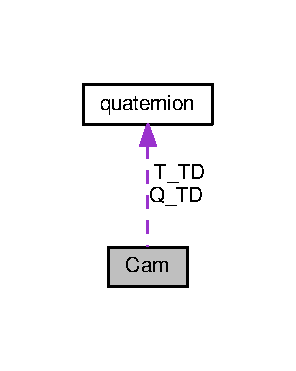
\includegraphics[width=142pt]{structCam__coll__graph}
\end{center}
\end{figure}
\subsubsection*{Public Attributes}
\begin{DoxyCompactItemize}
\item 
float \hyperlink{structCam_a99a4c54ed1a408665a0963f308008ec8}{scale}
\begin{DoxyCompactList}\small\item\em Depth scale ( $ \textit{m}$) \end{DoxyCompactList}\end{DoxyCompactItemize}
\begin{Indent}{\bf Focal length (pixels)}\par
\begin{DoxyCompactItemize}
\item 
float \hyperlink{structCam_a7d82658b0f9a7df54516cffb6d67ac07}{fx}
\item 
float \hyperlink{structCam_a2c80b4688fa8d02ad6c645246b6ea0d4}{fy}
\end{DoxyCompactItemize}
\end{Indent}
\begin{Indent}{\bf Image Center (pixels)}\par
\begin{DoxyCompactItemize}
\item 
float \hyperlink{structCam_a0d44db9d2a2e8c416cbf9cd30b6cd6f1}{ppx}
\item 
float \hyperlink{structCam_a5af4cee2ad3b008befb9626990dfbff2}{ppy}
\end{DoxyCompactItemize}
\end{Indent}
\begin{Indent}{\bf T265 to D435 Extrinsics}\par
\begin{DoxyCompactItemize}
\item 
\hyperlink{classquaternion}{quaternion} \hyperlink{structCam_a8b6ed5501753ad64cf3e36f798fbf3cd}{Q\+\_\+\+TD}
\item 
\hyperlink{classquaternion}{quaternion} \hyperlink{structCam_a05f5a946647cd44a473b0fd03186ca96}{T\+\_\+\+TD}
\end{DoxyCompactItemize}
\end{Indent}


\subsubsection{Detailed Description}
\hyperlink{classCamera}{Camera} Intrinsics and Extrinsics. 

Used to pass to C\+U\+DA kernel 

Definition at line \hyperlink{Voxel_8cuh_source_l00130}{130} of file \hyperlink{Voxel_8cuh_source}{Voxel.\+cuh}.



\subsubsection{Member Data Documentation}
\index{Cam@{Cam}!fx@{fx}}
\index{fx@{fx}!Cam@{Cam}}
\paragraph[{\texorpdfstring{fx}{fx}}]{\setlength{\rightskip}{0pt plus 5cm}float Cam\+::fx}\hypertarget{structCam_a7d82658b0f9a7df54516cffb6d67ac07}{}\label{structCam_a7d82658b0f9a7df54516cffb6d67ac07}


Definition at line \hyperlink{Voxel_8cuh_source_l00135}{135} of file \hyperlink{Voxel_8cuh_source}{Voxel.\+cuh}.

\index{Cam@{Cam}!fy@{fy}}
\index{fy@{fy}!Cam@{Cam}}
\paragraph[{\texorpdfstring{fy}{fy}}]{\setlength{\rightskip}{0pt plus 5cm}float Cam\+::fy}\hypertarget{structCam_a2c80b4688fa8d02ad6c645246b6ea0d4}{}\label{structCam_a2c80b4688fa8d02ad6c645246b6ea0d4}


Definition at line \hyperlink{Voxel_8cuh_source_l00135}{135} of file \hyperlink{Voxel_8cuh_source}{Voxel.\+cuh}.

\index{Cam@{Cam}!ppx@{ppx}}
\index{ppx@{ppx}!Cam@{Cam}}
\paragraph[{\texorpdfstring{ppx}{ppx}}]{\setlength{\rightskip}{0pt plus 5cm}float Cam\+::ppx}\hypertarget{structCam_a0d44db9d2a2e8c416cbf9cd30b6cd6f1}{}\label{structCam_a0d44db9d2a2e8c416cbf9cd30b6cd6f1}


Definition at line \hyperlink{Voxel_8cuh_source_l00141}{141} of file \hyperlink{Voxel_8cuh_source}{Voxel.\+cuh}.

\index{Cam@{Cam}!ppy@{ppy}}
\index{ppy@{ppy}!Cam@{Cam}}
\paragraph[{\texorpdfstring{ppy}{ppy}}]{\setlength{\rightskip}{0pt plus 5cm}float Cam\+::ppy}\hypertarget{structCam_a5af4cee2ad3b008befb9626990dfbff2}{}\label{structCam_a5af4cee2ad3b008befb9626990dfbff2}


Definition at line \hyperlink{Voxel_8cuh_source_l00141}{141} of file \hyperlink{Voxel_8cuh_source}{Voxel.\+cuh}.

\index{Cam@{Cam}!Q\+\_\+\+TD@{Q\+\_\+\+TD}}
\index{Q\+\_\+\+TD@{Q\+\_\+\+TD}!Cam@{Cam}}
\paragraph[{\texorpdfstring{Q\+\_\+\+TD}{Q_TD}}]{\setlength{\rightskip}{0pt plus 5cm}{\bf quaternion} Cam\+::\+Q\+\_\+\+TD}\hypertarget{structCam_a8b6ed5501753ad64cf3e36f798fbf3cd}{}\label{structCam_a8b6ed5501753ad64cf3e36f798fbf3cd}


Definition at line \hyperlink{Voxel_8cuh_source_l00150}{150} of file \hyperlink{Voxel_8cuh_source}{Voxel.\+cuh}.

\index{Cam@{Cam}!scale@{scale}}
\index{scale@{scale}!Cam@{Cam}}
\paragraph[{\texorpdfstring{scale}{scale}}]{\setlength{\rightskip}{0pt plus 5cm}float Cam\+::scale}\hypertarget{structCam_a99a4c54ed1a408665a0963f308008ec8}{}\label{structCam_a99a4c54ed1a408665a0963f308008ec8}


Depth scale ( $ \textit{m}$) 



Definition at line \hyperlink{Voxel_8cuh_source_l00145}{145} of file \hyperlink{Voxel_8cuh_source}{Voxel.\+cuh}.

\index{Cam@{Cam}!T\+\_\+\+TD@{T\+\_\+\+TD}}
\index{T\+\_\+\+TD@{T\+\_\+\+TD}!Cam@{Cam}}
\paragraph[{\texorpdfstring{T\+\_\+\+TD}{T_TD}}]{\setlength{\rightskip}{0pt plus 5cm}{\bf quaternion} Cam\+::\+T\+\_\+\+TD}\hypertarget{structCam_a05f5a946647cd44a473b0fd03186ca96}{}\label{structCam_a05f5a946647cd44a473b0fd03186ca96}


Definition at line \hyperlink{Voxel_8cuh_source_l00150}{150} of file \hyperlink{Voxel_8cuh_source}{Voxel.\+cuh}.



The documentation for this struct was generated from the following file\+:\begin{DoxyCompactItemize}
\item 
include/\hyperlink{Voxel_8cuh}{Voxel.\+cuh}\end{DoxyCompactItemize}

\hypertarget{classCamera}{}\subsection{Camera Class Reference}
\label{classCamera}\index{Camera@{Camera}}


\hyperlink{classCamera}{Camera} streams abstraction class.  




{\ttfamily \#include $<$Camera.\+hpp$>$}



Collaboration diagram for Camera\+:\nopagebreak
\begin{figure}[H]
\begin{center}
\leavevmode
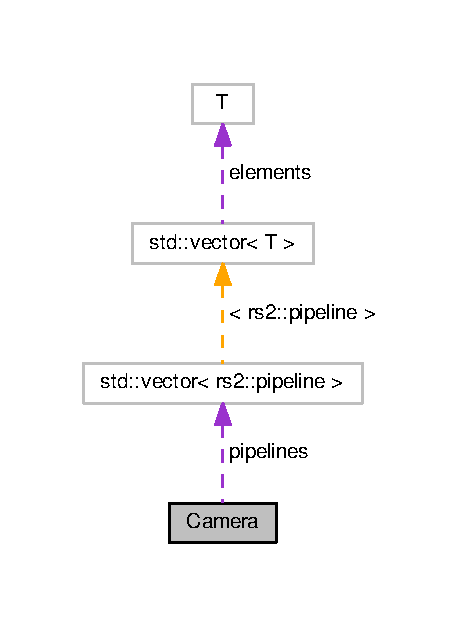
\includegraphics[width=221pt]{classCamera__coll__graph}
\end{center}
\end{figure}
\subsubsection*{Public Member Functions}
\begin{DoxyCompactItemize}
\item 
\hyperlink{classCamera_a01f94c3543f56ede7af49dc778f19331}{Camera} ()
\begin{DoxyCompactList}\small\item\em Default Constructor. \end{DoxyCompactList}\item 
\hyperlink{structBool__Init}{Bool\+\_\+\+Init} \hyperlink{classCamera_a7f09b843d9b3a97e78eefcebbc53e054}{Init} ()
\begin{DoxyCompactList}\small\item\em Initialize and start camera streams. \end{DoxyCompactList}\end{DoxyCompactItemize}
\subsubsection*{Public Attributes}
\begin{DoxyCompactItemize}
\item 
std\+::vector$<$ rs2\+::pipeline $>$ \hyperlink{classCamera_a689d4141375d8f7fbf1651338c1ea9c0}{pipelines}
\begin{DoxyCompactList}\small\item\em Used to call wait\+\_\+for\+\_\+frames() \end{DoxyCompactList}\item 
int \hyperlink{classCamera_a3061c56d262cab256468f05b9d8838fc}{model}
\begin{DoxyCompactList}\small\item\em Distortion model type. \end{DoxyCompactList}\item 
float \hyperlink{classCamera_af6b42da84223170eb6434a3df1d677af}{coeffs} \mbox{[}5\mbox{]}
\begin{DoxyCompactList}\small\item\em Distortion Coefficients. \end{DoxyCompactList}\end{DoxyCompactItemize}
\begin{Indent}{\bf D435 Intrinsics}\par
{\em Depth camera properties }\begin{DoxyCompactItemize}
\item 
float \hyperlink{classCamera_a50152f7c8f2ce7601dd6086c90b3a65c}{scale}
\begin{DoxyCompactList}\small\item\em Depth scale (m) \end{DoxyCompactList}\item 
float \hyperlink{classCamera_a4f5e789525c1c9306028c080922582e2}{fx}
\begin{DoxyCompactList}\small\item\em Focal length\+: x (pixels) \end{DoxyCompactList}\item 
float \hyperlink{classCamera_a1472650e23f3df5f23dda7f94537e889}{fy}
\begin{DoxyCompactList}\small\item\em Focal length\+: y (pixels) \end{DoxyCompactList}\end{DoxyCompactItemize}
\end{Indent}
{\bf }\par
\begin{DoxyCompactItemize}
\item 
float \hyperlink{classCamera_aa646a2de04e9ad37395dcf3c4a171abe}{ppx}
\begin{DoxyCompactList}\small\item\em Image center\+: x (pixels) \end{DoxyCompactList}\item 
float \hyperlink{classCamera_a0e51f157264b9c9e18feb584c5a6c606}{ppy}
\begin{DoxyCompactList}\small\item\em Image center\+: y (pixels) \end{DoxyCompactList}\end{DoxyCompactItemize}

\begin{Indent}{\bf Frame Queue}\par
{\em Frame queues for tracking and depth }\begin{DoxyCompactItemize}
\item 
rs2\+::frame\+\_\+queue \hyperlink{classCamera_a84a3a043e61b967fb1dc6fbe62bf33aa}{d\+\_\+queue}
\item 
rs2\+::frame\+\_\+queue \hyperlink{classCamera_ad8a4c52c0ae125ab8ca66902408f5e95}{t\+\_\+queue}
\end{DoxyCompactItemize}
\end{Indent}
\subsubsection*{Private Attributes}
\begin{DoxyCompactItemize}
\item 
rs2\+::context \hyperlink{classCamera_a4373bc8793e3bb1d6eb2cca3eb25a31e}{ctx}
\begin{DoxyCompactList}\small\item\em Realsense context object. \end{DoxyCompactList}\end{DoxyCompactItemize}


\subsubsection{Detailed Description}
\hyperlink{classCamera}{Camera} streams abstraction class. 

This class is used to initialize the D435 -\/ Depth camera, and T265 -\/ Tracking camera. The class object can either be used directly, or used along with Cam\+\_\+\+R\+W.\+hpp as a publisher. All device properties can be modified in this class. \begin{DoxySeeAlso}{See also}
Cam\+\_\+\+R\+W.\+hpp 
\end{DoxySeeAlso}


Definition at line \hyperlink{Camera_8hpp_source_l00069}{69} of file \hyperlink{Camera_8hpp_source}{Camera.\+hpp}.



\subsubsection{Constructor \& Destructor Documentation}
\index{Camera@{Camera}!Camera@{Camera}}
\index{Camera@{Camera}!Camera@{Camera}}
\paragraph[{\texorpdfstring{Camera()}{Camera()}}]{\setlength{\rightskip}{0pt plus 5cm}Camera\+::\+Camera (
\begin{DoxyParamCaption}
{}
\end{DoxyParamCaption}
)\hspace{0.3cm}{\ttfamily [inline]}}\hypertarget{classCamera_a01f94c3543f56ede7af49dc778f19331}{}\label{classCamera_a01f94c3543f56ede7af49dc778f19331}


Default Constructor. 

Initializes the Queues with a size of B\+U\+F\+F\+E\+R\+\_\+\+L\+E\+N\+G\+TH \begin{DoxySeeAlso}{See also}
\hyperlink{Camera_8hpp_af7b7dc9a200cb1404c280bd500fd1551}{B\+U\+F\+F\+E\+R\+\_\+\+L\+E\+N\+G\+TH} 
\end{DoxySeeAlso}


Definition at line \hyperlink{Camera_8hpp_source_l00124}{124} of file \hyperlink{Camera_8hpp_source}{Camera.\+hpp}.



\subsubsection{Member Function Documentation}
\index{Camera@{Camera}!Init@{Init}}
\index{Init@{Init}!Camera@{Camera}}
\paragraph[{\texorpdfstring{Init()}{Init()}}]{\setlength{\rightskip}{0pt plus 5cm}{\bf Bool\+\_\+\+Init} Camera\+::\+Init (
\begin{DoxyParamCaption}
{}
\end{DoxyParamCaption}
)\hspace{0.3cm}{\ttfamily [inline]}}\hypertarget{classCamera_a7f09b843d9b3a97e78eefcebbc53e054}{}\label{classCamera_a7f09b843d9b3a97e78eefcebbc53e054}


Initialize and start camera streams. 

Properties of the streams are set in this method. ~\newline
 D435\+: Currently only Depth image is streamed. Image dimensions, bit depth, and F\+PS of D435 can be set in this method. ~\newline
 T265\+: Currently only 6-\/\+DoF \hyperlink{structPose}{Pose} is streamed. The Degrees of Freedom of \hyperlink{structPose}{Pose} can be set in this method. run rs-\/enumerate-\/devices in terminal to view available configurations ~\newline
 N\+O\+TE\+: The serial number is different for every camera (even for the same model). This param should be set for every new device. \begin{DoxySeeAlso}{See also}
\hyperlink{Camera_8hpp_a66326676d44c838441a4dc39c85f599b}{w}, \hyperlink{Camera_8hpp_a3f40fea9b1040e381f08ddd4b026765d}{h}, \hyperlink{Camera_8hpp_ad56e71b7cc91ce32f920769b6eb31e03}{d\+\_\+fps}, \hyperlink{Camera_8hpp_a08da237113fcf4a0fb79c89a2ba02bce}{D\+E\+P\+T\+H\+\_\+\+S\+NO}, \hyperlink{Camera_8hpp_a97168636c8d72f641dc410554a42b2ec}{T\+R\+A\+C\+K\+\_\+\+S\+NO}, \hyperlink{structBool__Init}{Bool\+\_\+\+Init} 
\end{DoxySeeAlso}
\begin{DoxyReturn}{Returns}
a \hyperlink{structBool__Init}{Bool\+\_\+\+Init} struct stating which cameras where initialzed. 
\end{DoxyReturn}


Definition at line \hyperlink{Camera_8hpp_source_l00135}{135} of file \hyperlink{Camera_8hpp_source}{Camera.\+hpp}.



Here is the caller graph for this function\+:\nopagebreak
\begin{figure}[H]
\begin{center}
\leavevmode
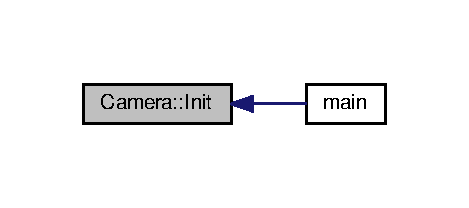
\includegraphics[width=225pt]{classCamera_a7f09b843d9b3a97e78eefcebbc53e054_icgraph}
\end{center}
\end{figure}




\subsubsection{Member Data Documentation}
\index{Camera@{Camera}!coeffs@{coeffs}}
\index{coeffs@{coeffs}!Camera@{Camera}}
\paragraph[{\texorpdfstring{coeffs}{coeffs}}]{\setlength{\rightskip}{0pt plus 5cm}float Camera\+::coeffs\mbox{[}5\mbox{]}}\hypertarget{classCamera_af6b42da84223170eb6434a3df1d677af}{}\label{classCamera_af6b42da84223170eb6434a3df1d677af}


Distortion Coefficients. 



Definition at line \hyperlink{Camera_8hpp_source_l00107}{107} of file \hyperlink{Camera_8hpp_source}{Camera.\+hpp}.

\index{Camera@{Camera}!ctx@{ctx}}
\index{ctx@{ctx}!Camera@{Camera}}
\paragraph[{\texorpdfstring{ctx}{ctx}}]{\setlength{\rightskip}{0pt plus 5cm}rs2\+::context Camera\+::ctx\hspace{0.3cm}{\ttfamily [private]}}\hypertarget{classCamera_a4373bc8793e3bb1d6eb2cca3eb25a31e}{}\label{classCamera_a4373bc8793e3bb1d6eb2cca3eb25a31e}


Realsense context object. 

The members of this object can be set and passed to rs2\+::pipeline constructor to set the properties of the cameras. 

Definition at line \hyperlink{Camera_8hpp_source_l00076}{76} of file \hyperlink{Camera_8hpp_source}{Camera.\+hpp}.

\index{Camera@{Camera}!d\+\_\+queue@{d\+\_\+queue}}
\index{d\+\_\+queue@{d\+\_\+queue}!Camera@{Camera}}
\paragraph[{\texorpdfstring{d\+\_\+queue}{d_queue}}]{\setlength{\rightskip}{0pt plus 5cm}rs2\+::frame\+\_\+queue Camera\+::d\+\_\+queue}\hypertarget{classCamera_a84a3a043e61b967fb1dc6fbe62bf33aa}{}\label{classCamera_a84a3a043e61b967fb1dc6fbe62bf33aa}
Queue for Depth frames 

Definition at line \hyperlink{Camera_8hpp_source_l00115}{115} of file \hyperlink{Camera_8hpp_source}{Camera.\+hpp}.

\index{Camera@{Camera}!fx@{fx}}
\index{fx@{fx}!Camera@{Camera}}
\paragraph[{\texorpdfstring{fx}{fx}}]{\setlength{\rightskip}{0pt plus 5cm}float Camera\+::fx}\hypertarget{classCamera_a4f5e789525c1c9306028c080922582e2}{}\label{classCamera_a4f5e789525c1c9306028c080922582e2}


Focal length\+: x (pixels) 



Definition at line \hyperlink{Camera_8hpp_source_l00094}{94} of file \hyperlink{Camera_8hpp_source}{Camera.\+hpp}.

\index{Camera@{Camera}!fy@{fy}}
\index{fy@{fy}!Camera@{Camera}}
\paragraph[{\texorpdfstring{fy}{fy}}]{\setlength{\rightskip}{0pt plus 5cm}float Camera\+::fy}\hypertarget{classCamera_a1472650e23f3df5f23dda7f94537e889}{}\label{classCamera_a1472650e23f3df5f23dda7f94537e889}


Focal length\+: y (pixels) 



Definition at line \hyperlink{Camera_8hpp_source_l00096}{96} of file \hyperlink{Camera_8hpp_source}{Camera.\+hpp}.

\index{Camera@{Camera}!model@{model}}
\index{model@{model}!Camera@{Camera}}
\paragraph[{\texorpdfstring{model}{model}}]{\setlength{\rightskip}{0pt plus 5cm}int Camera\+::model}\hypertarget{classCamera_a3061c56d262cab256468f05b9d8838fc}{}\label{classCamera_a3061c56d262cab256468f05b9d8838fc}


Distortion model type. 



Definition at line \hyperlink{Camera_8hpp_source_l00105}{105} of file \hyperlink{Camera_8hpp_source}{Camera.\+hpp}.

\index{Camera@{Camera}!pipelines@{pipelines}}
\index{pipelines@{pipelines}!Camera@{Camera}}
\paragraph[{\texorpdfstring{pipelines}{pipelines}}]{\setlength{\rightskip}{0pt plus 5cm}std\+::vector$<$rs2\+::pipeline$>$ Camera\+::pipelines}\hypertarget{classCamera_a689d4141375d8f7fbf1651338c1ea9c0}{}\label{classCamera_a689d4141375d8f7fbf1651338c1ea9c0}


Used to call wait\+\_\+for\+\_\+frames() 

Elements of this vector can be used to wait for frames. If only camera is attached, the vector contains only one element. If both cameras are attached, the first element is for T265 and the second for D435 

Definition at line \hyperlink{Camera_8hpp_source_l00085}{85} of file \hyperlink{Camera_8hpp_source}{Camera.\+hpp}.

\index{Camera@{Camera}!ppx@{ppx}}
\index{ppx@{ppx}!Camera@{Camera}}
\paragraph[{\texorpdfstring{ppx}{ppx}}]{\setlength{\rightskip}{0pt plus 5cm}float Camera\+::ppx}\hypertarget{classCamera_aa646a2de04e9ad37395dcf3c4a171abe}{}\label{classCamera_aa646a2de04e9ad37395dcf3c4a171abe}


Image center\+: x (pixels) 



Definition at line \hyperlink{Camera_8hpp_source_l00100}{100} of file \hyperlink{Camera_8hpp_source}{Camera.\+hpp}.

\index{Camera@{Camera}!ppy@{ppy}}
\index{ppy@{ppy}!Camera@{Camera}}
\paragraph[{\texorpdfstring{ppy}{ppy}}]{\setlength{\rightskip}{0pt plus 5cm}float Camera\+::ppy}\hypertarget{classCamera_a0e51f157264b9c9e18feb584c5a6c606}{}\label{classCamera_a0e51f157264b9c9e18feb584c5a6c606}


Image center\+: y (pixels) 



Definition at line \hyperlink{Camera_8hpp_source_l00102}{102} of file \hyperlink{Camera_8hpp_source}{Camera.\+hpp}.

\index{Camera@{Camera}!scale@{scale}}
\index{scale@{scale}!Camera@{Camera}}
\paragraph[{\texorpdfstring{scale}{scale}}]{\setlength{\rightskip}{0pt plus 5cm}float Camera\+::scale}\hypertarget{classCamera_a50152f7c8f2ce7601dd6086c90b3a65c}{}\label{classCamera_a50152f7c8f2ce7601dd6086c90b3a65c}


Depth scale (m) 



Definition at line \hyperlink{Camera_8hpp_source_l00091}{91} of file \hyperlink{Camera_8hpp_source}{Camera.\+hpp}.

\index{Camera@{Camera}!t\+\_\+queue@{t\+\_\+queue}}
\index{t\+\_\+queue@{t\+\_\+queue}!Camera@{Camera}}
\paragraph[{\texorpdfstring{t\+\_\+queue}{t_queue}}]{\setlength{\rightskip}{0pt plus 5cm}rs2\+::frame\+\_\+queue Camera\+::t\+\_\+queue}\hypertarget{classCamera_ad8a4c52c0ae125ab8ca66902408f5e95}{}\label{classCamera_ad8a4c52c0ae125ab8ca66902408f5e95}
Queue for \hyperlink{structPose}{Pose} frames 

Definition at line \hyperlink{Camera_8hpp_source_l00117}{117} of file \hyperlink{Camera_8hpp_source}{Camera.\+hpp}.



The documentation for this class was generated from the following file\+:\begin{DoxyCompactItemize}
\item 
include/\hyperlink{Camera_8hpp}{Camera.\+hpp}\end{DoxyCompactItemize}

\hypertarget{classCPU__FE}{}\subsection{C\+P\+U\+\_\+\+FE Class Reference}
\label{classCPU__FE}\index{C\+P\+U\+\_\+\+FE@{C\+P\+U\+\_\+\+FE}}


Wrapper class for \hyperlink{classocc__grid}{occ\+\_\+grid}.  




{\ttfamily \#include $<$Voxel.\+hpp$>$}



Inheritance diagram for C\+P\+U\+\_\+\+FE\+:\nopagebreak
\begin{figure}[H]
\begin{center}
\leavevmode
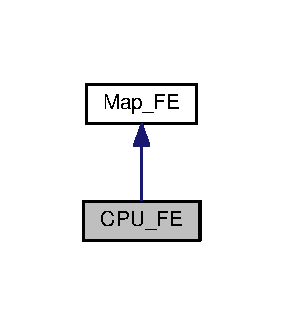
\includegraphics[width=136pt]{classCPU__FE__inherit__graph}
\end{center}
\end{figure}


Collaboration diagram for C\+P\+U\+\_\+\+FE\+:\nopagebreak
\begin{figure}[H]
\begin{center}
\leavevmode
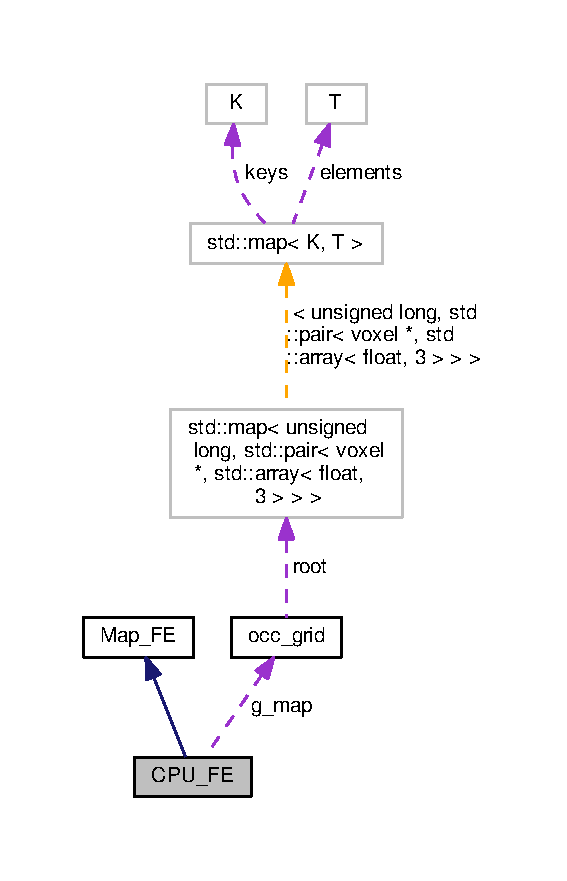
\includegraphics[width=272pt]{classCPU__FE__coll__graph}
\end{center}
\end{figure}
\subsubsection*{Public Member Functions}
\begin{DoxyCompactItemize}
\item 
\hyperlink{classCPU__FE_a17780bbe106fb8f752e06987b5eefc7f}{C\+P\+U\+\_\+\+FE} ()
\begin{DoxyCompactList}\small\item\em Default Constructor. \end{DoxyCompactList}\item 
void \hyperlink{classCPU__FE_aae7cb60a405b294a680a929ecff5c2ae}{Update} (\hyperlink{classCamera}{Camera} const \&C, rs2\+\_\+pose const \&pose, cv\+::\+Mat const \&depth)
\begin{DoxyCompactList}\small\item\em Updates the measurement data in the global map. \end{DoxyCompactList}\item 
void \hyperlink{classCPU__FE_a4b085e590daa33cf1e2f100a58236009}{Points} (std\+::vector$<$ std\+::tuple$<$ float, float, float, float $>$ $>$ $\ast$points)
\begin{DoxyCompactList}\small\item\em Appends all points in global map to the vector. \end{DoxyCompactList}\item 
\hyperlink{classCPU__FE_a425dc3014e22d7aeaaf261ac945f4da1}{$\sim$\+C\+P\+U\+\_\+\+FE} ()
\begin{DoxyCompactList}\small\item\em Destructor. \end{DoxyCompactList}\end{DoxyCompactItemize}
\subsubsection*{Private Attributes}
\begin{DoxyCompactItemize}
\item 
\hyperlink{classocc__grid}{occ\+\_\+grid} $\ast$ \hyperlink{classCPU__FE_ad3779fc0a23127e425d8f0fc3c2661dc}{g\+\_\+map}
\begin{DoxyCompactList}\small\item\em Global map object. \end{DoxyCompactList}\end{DoxyCompactItemize}


\subsubsection{Detailed Description}
Wrapper class for \hyperlink{classocc__grid}{occ\+\_\+grid}. 

This class acts as an abstraction for the \hyperlink{classocc__grid}{occ\+\_\+grid} class. Also inherits virtual class \hyperlink{classMap__FE}{Map\+\_\+\+FE}, so implements all its virtual methods. \begin{DoxySeeAlso}{See also}
\hyperlink{classMap__FE}{Map\+\_\+\+FE} 
\end{DoxySeeAlso}


Definition at line \hyperlink{Voxel_8hpp_source_l00460}{460} of file \hyperlink{Voxel_8hpp_source}{Voxel.\+hpp}.



\subsubsection{Constructor \& Destructor Documentation}
\index{C\+P\+U\+\_\+\+FE@{C\+P\+U\+\_\+\+FE}!C\+P\+U\+\_\+\+FE@{C\+P\+U\+\_\+\+FE}}
\index{C\+P\+U\+\_\+\+FE@{C\+P\+U\+\_\+\+FE}!C\+P\+U\+\_\+\+FE@{C\+P\+U\+\_\+\+FE}}
\paragraph[{\texorpdfstring{C\+P\+U\+\_\+\+F\+E()}{CPU_FE()}}]{\setlength{\rightskip}{0pt plus 5cm}C\+P\+U\+\_\+\+F\+E\+::\+C\+P\+U\+\_\+\+FE (
\begin{DoxyParamCaption}
{}
\end{DoxyParamCaption}
)\hspace{0.3cm}{\ttfamily [inline]}}\hypertarget{classCPU__FE_a17780bbe106fb8f752e06987b5eefc7f}{}\label{classCPU__FE_a17780bbe106fb8f752e06987b5eefc7f}


Default Constructor. 



Definition at line \hyperlink{Voxel_8hpp_source_l00472}{472} of file \hyperlink{Voxel_8hpp_source}{Voxel.\+hpp}.

\index{C\+P\+U\+\_\+\+FE@{C\+P\+U\+\_\+\+FE}!````~C\+P\+U\+\_\+\+FE@{$\sim$\+C\+P\+U\+\_\+\+FE}}
\index{````~C\+P\+U\+\_\+\+FE@{$\sim$\+C\+P\+U\+\_\+\+FE}!C\+P\+U\+\_\+\+FE@{C\+P\+U\+\_\+\+FE}}
\paragraph[{\texorpdfstring{$\sim$\+C\+P\+U\+\_\+\+F\+E()}{~CPU_FE()}}]{\setlength{\rightskip}{0pt plus 5cm}C\+P\+U\+\_\+\+F\+E\+::$\sim$\+C\+P\+U\+\_\+\+FE (
\begin{DoxyParamCaption}
{}
\end{DoxyParamCaption}
)\hspace{0.3cm}{\ttfamily [inline]}}\hypertarget{classCPU__FE_a425dc3014e22d7aeaaf261ac945f4da1}{}\label{classCPU__FE_a425dc3014e22d7aeaaf261ac945f4da1}


Destructor. 

Deletes the global map \begin{DoxySeeAlso}{See also}
\hyperlink{classocc__grid_adbfab59a1fb247d53a993fd9a2a26d67}{occ\+\_\+grid\+::free\+\_\+mem()} 
\end{DoxySeeAlso}


Definition at line \hyperlink{Voxel_8hpp_source_l00518}{518} of file \hyperlink{Voxel_8hpp_source}{Voxel.\+hpp}.



Here is the call graph for this function\+:\nopagebreak
\begin{figure}[H]
\begin{center}
\leavevmode
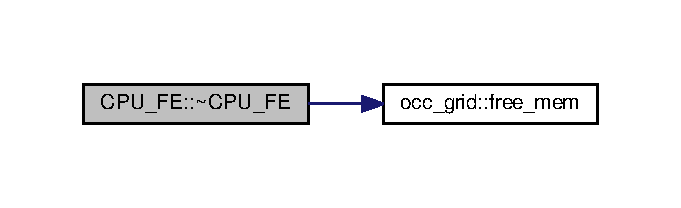
\includegraphics[width=327pt]{classCPU__FE_a425dc3014e22d7aeaaf261ac945f4da1_cgraph}
\end{center}
\end{figure}




\subsubsection{Member Function Documentation}
\index{C\+P\+U\+\_\+\+FE@{C\+P\+U\+\_\+\+FE}!Points@{Points}}
\index{Points@{Points}!C\+P\+U\+\_\+\+FE@{C\+P\+U\+\_\+\+FE}}
\paragraph[{\texorpdfstring{Points(std\+::vector$<$ std\+::tuple$<$ float, float, float, float $>$ $>$ $\ast$points)}{Points(std::vector< std::tuple< float, float, float, float > > *points)}}]{\setlength{\rightskip}{0pt plus 5cm}void C\+P\+U\+\_\+\+F\+E\+::\+Points (
\begin{DoxyParamCaption}
\item[{std\+::vector$<$ std\+::tuple$<$ float, float, float, float $>$ $>$ $\ast$}]{points}
\end{DoxyParamCaption}
)\hspace{0.3cm}{\ttfamily [inline]}, {\ttfamily [virtual]}}\hypertarget{classCPU__FE_a4b085e590daa33cf1e2f100a58236009}{}\label{classCPU__FE_a4b085e590daa33cf1e2f100a58236009}


Appends all points in global map to the vector. 


\begin{DoxyParams}{Parameters}
{\em vector} & of points \\
\hline
\end{DoxyParams}
\begin{DoxySeeAlso}{See also}
\hyperlink{classocc__grid_a8b47af213fb57bf31c21ab1a9ef36505}{occ\+\_\+grid\+::all\+\_\+points()}, \hyperlink{classMap__FE_aedfee41631a7287c9eb377ccb05317d6}{Map\+\_\+\+F\+E\+::\+Points()} 
\end{DoxySeeAlso}


Implements \hyperlink{classMap__FE_aedfee41631a7287c9eb377ccb05317d6}{Map\+\_\+\+FE}.



Definition at line \hyperlink{Voxel_8hpp_source_l00510}{510} of file \hyperlink{Voxel_8hpp_source}{Voxel.\+hpp}.



Here is the call graph for this function\+:\nopagebreak
\begin{figure}[H]
\begin{center}
\leavevmode
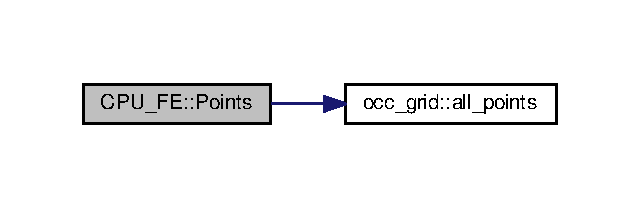
\includegraphics[width=307pt]{classCPU__FE_a4b085e590daa33cf1e2f100a58236009_cgraph}
\end{center}
\end{figure}


\index{C\+P\+U\+\_\+\+FE@{C\+P\+U\+\_\+\+FE}!Update@{Update}}
\index{Update@{Update}!C\+P\+U\+\_\+\+FE@{C\+P\+U\+\_\+\+FE}}
\paragraph[{\texorpdfstring{Update(\+Camera const \&\+C, rs2\+\_\+pose const \&pose, cv\+::\+Mat const \&depth)}{Update(Camera const &C, rs2_pose const &pose, cv::Mat const &depth)}}]{\setlength{\rightskip}{0pt plus 5cm}void C\+P\+U\+\_\+\+F\+E\+::\+Update (
\begin{DoxyParamCaption}
\item[{{\bf Camera} const \&}]{C, }
\item[{rs2\+\_\+pose const \&}]{pose, }
\item[{cv\+::\+Mat const \&}]{depth}
\end{DoxyParamCaption}
)\hspace{0.3cm}{\ttfamily [inline]}, {\ttfamily [virtual]}}\hypertarget{classCPU__FE_aae7cb60a405b294a680a929ecff5c2ae}{}\label{classCPU__FE_aae7cb60a405b294a680a929ecff5c2ae}


Updates the measurement data in the global map. 

Sequencially calls \hyperlink{classocc__grid_aaf38d339d7d1b3226d9673f8d6102b2c}{occ\+\_\+grid\+::update\+\_\+point()} on all points in the depth image. The co-\/ordinates are transformed from the D435 frame to T265 global frame and then passed on to \hyperlink{classocc__grid_aaf38d339d7d1b3226d9673f8d6102b2c}{occ\+\_\+grid\+::update\+\_\+point()}. 
\begin{DoxyParams}{Parameters}
{\em \hyperlink{classCamera}{Camera}} & object \\
\hline
{\em pose} & of T265 \\
\hline
{\em 16-\/bit} & D435 depth image \\
\hline
\end{DoxyParams}
\begin{DoxySeeAlso}{See also}
\hyperlink{classocc__grid_aaf38d339d7d1b3226d9673f8d6102b2c}{occ\+\_\+grid\+::update\+\_\+point()}, \hyperlink{classMap__FE_a901af5011ef87bfd1dac3e568ef29c47}{Map\+\_\+\+F\+E\+::\+Update()} 
\end{DoxySeeAlso}


Implements \hyperlink{classMap__FE_a901af5011ef87bfd1dac3e568ef29c47}{Map\+\_\+\+FE}.



Definition at line \hyperlink{Voxel_8hpp_source_l00484}{484} of file \hyperlink{Voxel_8hpp_source}{Voxel.\+hpp}.



Here is the call graph for this function\+:\nopagebreak
\begin{figure}[H]
\begin{center}
\leavevmode
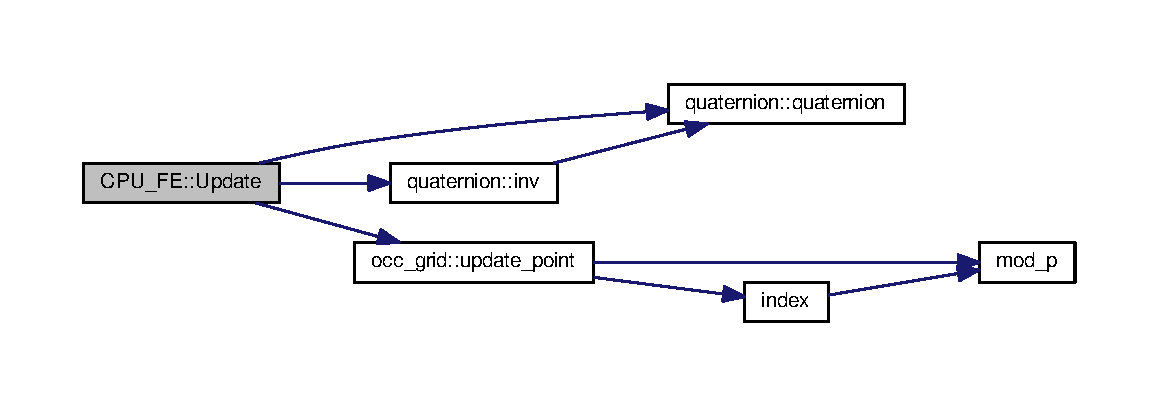
\includegraphics[width=350pt]{classCPU__FE_aae7cb60a405b294a680a929ecff5c2ae_cgraph}
\end{center}
\end{figure}




\subsubsection{Member Data Documentation}
\index{C\+P\+U\+\_\+\+FE@{C\+P\+U\+\_\+\+FE}!g\+\_\+map@{g\+\_\+map}}
\index{g\+\_\+map@{g\+\_\+map}!C\+P\+U\+\_\+\+FE@{C\+P\+U\+\_\+\+FE}}
\paragraph[{\texorpdfstring{g\+\_\+map}{g_map}}]{\setlength{\rightskip}{0pt plus 5cm}{\bf occ\+\_\+grid}$\ast$ C\+P\+U\+\_\+\+F\+E\+::g\+\_\+map\hspace{0.3cm}{\ttfamily [private]}}\hypertarget{classCPU__FE_ad3779fc0a23127e425d8f0fc3c2661dc}{}\label{classCPU__FE_ad3779fc0a23127e425d8f0fc3c2661dc}


Global map object. 

\begin{DoxySeeAlso}{See also}
\hyperlink{classocc__grid}{occ\+\_\+grid} 
\end{DoxySeeAlso}


Definition at line \hyperlink{Voxel_8hpp_source_l00467}{467} of file \hyperlink{Voxel_8hpp_source}{Voxel.\+hpp}.



The documentation for this class was generated from the following file\+:\begin{DoxyCompactItemize}
\item 
include/\hyperlink{Voxel_8hpp}{Voxel.\+hpp}\end{DoxyCompactItemize}

\hypertarget{classGPU__FE}{}\subsection{G\+P\+U\+\_\+\+FE Class Reference}
\label{classGPU__FE}\index{G\+P\+U\+\_\+\+FE@{G\+P\+U\+\_\+\+FE}}


Wrapper class for \hyperlink{classocc__grid}{occ\+\_\+grid}.  




Inheritance diagram for G\+P\+U\+\_\+\+FE\+:\nopagebreak
\begin{figure}[H]
\begin{center}
\leavevmode
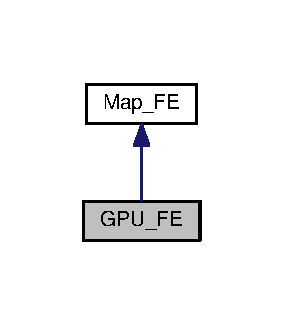
\includegraphics[width=136pt]{classGPU__FE__inherit__graph}
\end{center}
\end{figure}


Collaboration diagram for G\+P\+U\+\_\+\+FE\+:\nopagebreak
\begin{figure}[H]
\begin{center}
\leavevmode
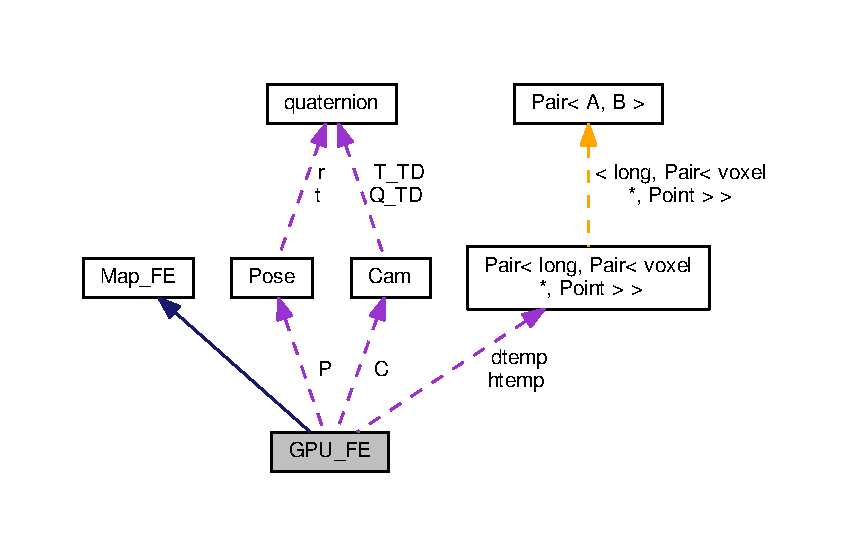
\includegraphics[width=350pt]{classGPU__FE__coll__graph}
\end{center}
\end{figure}
\subsubsection*{Public Member Functions}
\begin{DoxyCompactItemize}
\item 
\hyperlink{classGPU__FE_a2c2e9757a562ef8c33ce9fb474ae0742}{G\+P\+U\+\_\+\+FE} ()
\begin{DoxyCompactList}\small\item\em Default Constructor. \end{DoxyCompactList}\item 
void \hyperlink{classGPU__FE_aa9039bd613961d4e0911b8514ed14fba}{Update} (\hyperlink{classCamera}{Camera} const \&\hyperlink{classGPU__FE_aada926a7b999648bcb837507bf6a75d3}{C}, rs2\+\_\+pose const \&pose, cv\+::\+Mat const \&depth)
\begin{DoxyCompactList}\small\item\em Updates the measurement data in the global map. \end{DoxyCompactList}\item 
void \hyperlink{classGPU__FE_aea86626bdab826bc91b955ad6e5f6653}{Points} (std\+::vector$<$ std\+::tuple$<$ float, float, float, float $>$ $>$ $\ast$points)
\begin{DoxyCompactList}\small\item\em Appends all points in global map to the vector. \end{DoxyCompactList}\item 
\hyperlink{classGPU__FE_a1da80fa2f9f13df184e545e46f9d9270}{$\sim$\+G\+P\+U\+\_\+\+FE} ()
\begin{DoxyCompactList}\small\item\em Destructor. \end{DoxyCompactList}\end{DoxyCompactItemize}
\subsubsection*{Private Attributes}
\begin{DoxyCompactItemize}
\item 
thrust\+::host\+\_\+vector$<$ \hyperlink{classPair}{Pair}$<$ long, \hyperlink{classPair}{Pair}$<$ \hyperlink{classvoxel}{voxel} $\ast$, \hyperlink{structPoint}{Point} $>$ $>$ $>$ \hyperlink{classGPU__FE_a7418d50e4e22db3671d9c000344aaddc}{HV}
\begin{DoxyCompactList}\small\item\em Vector in host memory containing root voxels. \end{DoxyCompactList}\item 
long \hyperlink{classGPU__FE_a0bd3424bf1e7775fc5eef2d17714cd94}{s}
\begin{DoxyCompactList}\small\item\em Size of HV vector. \end{DoxyCompactList}\item 
\hyperlink{classPair}{Pair}$<$ long, \hyperlink{classPair}{Pair}$<$ \hyperlink{classvoxel}{voxel} $\ast$, \hyperlink{structPoint}{Point} $>$ $>$ $\ast$ \hyperlink{classGPU__FE_a15cab1132ca16d50844a60cc09235567}{dtemp}
\begin{DoxyCompactList}\small\item\em Temporary array stored in device memory. \end{DoxyCompactList}\item 
\hyperlink{classPair}{Pair}$<$ long, \hyperlink{classPair}{Pair}$<$ \hyperlink{classvoxel}{voxel} $\ast$, \hyperlink{structPoint}{Point} $>$ $>$ $\ast$ \hyperlink{classGPU__FE_afd39eabc36a87a6cde62b57296efcc8a}{htemp}
\begin{DoxyCompactList}\small\item\em Temporary array stored in host memory. \end{DoxyCompactList}\item 
unsigned short $\ast$ \hyperlink{classGPU__FE_a20be80d2f552afc21f97831fcc4983e9}{D}
\begin{DoxyCompactList}\small\item\em Pointer to depth image stored on device. \end{DoxyCompactList}\item 
\hyperlink{structPose}{Pose} $\ast$ \hyperlink{classGPU__FE_a1a99fc5bf3cc72c1d39f779e632f5fe7}{P}
\begin{DoxyCompactList}\small\item\em Pointer to \hyperlink{structPose}{Pose} struct stored on device. \end{DoxyCompactList}\item 
\hyperlink{structCam}{Cam} $\ast$ \hyperlink{classGPU__FE_aada926a7b999648bcb837507bf6a75d3}{C}
\begin{DoxyCompactList}\small\item\em Pointer ot \hyperlink{structCam}{Cam} struct stored on device. \end{DoxyCompactList}\item 
long $\ast$ \hyperlink{classGPU__FE_a1e2b5d0d82b739ab93b43e2bb862392a}{S}
\begin{DoxyCompactList}\small\item\em Size of HV vector; passed to device. \end{DoxyCompactList}\end{DoxyCompactItemize}


\subsubsection{Detailed Description}
Wrapper class for \hyperlink{classocc__grid}{occ\+\_\+grid}. 

This class acts as an abstraction for the C\+U\+DA kernel methods. Also inherits virtual class \hyperlink{classMap__FE}{Map\+\_\+\+FE}, so implements all its virtual methods. \begin{DoxySeeAlso}{See also}
\hyperlink{classMap__FE}{Map\+\_\+\+FE} 
\end{DoxySeeAlso}


Definition at line \hyperlink{Voxel_8cuh_source_l00603}{603} of file \hyperlink{Voxel_8cuh_source}{Voxel.\+cuh}.



\subsubsection{Constructor \& Destructor Documentation}
\index{G\+P\+U\+\_\+\+FE@{G\+P\+U\+\_\+\+FE}!G\+P\+U\+\_\+\+FE@{G\+P\+U\+\_\+\+FE}}
\index{G\+P\+U\+\_\+\+FE@{G\+P\+U\+\_\+\+FE}!G\+P\+U\+\_\+\+FE@{G\+P\+U\+\_\+\+FE}}
\paragraph[{\texorpdfstring{G\+P\+U\+\_\+\+F\+E()}{GPU_FE()}}]{\setlength{\rightskip}{0pt plus 5cm}G\+P\+U\+\_\+\+F\+E\+::\+G\+P\+U\+\_\+\+FE (
\begin{DoxyParamCaption}
{}
\end{DoxyParamCaption}
)\hspace{0.3cm}{\ttfamily [inline]}}\hypertarget{classGPU__FE_a2c2e9757a562ef8c33ce9fb474ae0742}{}\label{classGPU__FE_a2c2e9757a562ef8c33ce9fb474ae0742}


Default Constructor. 

Static memory required for the device members are allocated on device memory. Space for temporary array on host is allocated in host heap memory. 

Definition at line \hyperlink{Voxel_8cuh_source_l00638}{638} of file \hyperlink{Voxel_8cuh_source}{Voxel.\+cuh}.

\index{G\+P\+U\+\_\+\+FE@{G\+P\+U\+\_\+\+FE}!````~G\+P\+U\+\_\+\+FE@{$\sim$\+G\+P\+U\+\_\+\+FE}}
\index{````~G\+P\+U\+\_\+\+FE@{$\sim$\+G\+P\+U\+\_\+\+FE}!G\+P\+U\+\_\+\+FE@{G\+P\+U\+\_\+\+FE}}
\paragraph[{\texorpdfstring{$\sim$\+G\+P\+U\+\_\+\+F\+E()}{~GPU_FE()}}]{\setlength{\rightskip}{0pt plus 5cm}G\+P\+U\+\_\+\+F\+E\+::$\sim$\+G\+P\+U\+\_\+\+FE (
\begin{DoxyParamCaption}
{}
\end{DoxyParamCaption}
)\hspace{0.3cm}{\ttfamily [inline]}}\hypertarget{classGPU__FE_a1da80fa2f9f13df184e545e46f9d9270}{}\label{classGPU__FE_a1da80fa2f9f13df184e545e46f9d9270}


Destructor. 

Deletes the global map \begin{DoxySeeAlso}{See also}
Delete() 
\end{DoxySeeAlso}


Definition at line \hyperlink{Voxel_8cuh_source_l00729}{729} of file \hyperlink{Voxel_8cuh_source}{Voxel.\+cuh}.



\subsubsection{Member Function Documentation}
\index{G\+P\+U\+\_\+\+FE@{G\+P\+U\+\_\+\+FE}!Points@{Points}}
\index{Points@{Points}!G\+P\+U\+\_\+\+FE@{G\+P\+U\+\_\+\+FE}}
\paragraph[{\texorpdfstring{Points(std\+::vector$<$ std\+::tuple$<$ float, float, float, float $>$ $>$ $\ast$points)}{Points(std::vector< std::tuple< float, float, float, float > > *points)}}]{\setlength{\rightskip}{0pt plus 5cm}void G\+P\+U\+\_\+\+F\+E\+::\+Points (
\begin{DoxyParamCaption}
\item[{std\+::vector$<$ std\+::tuple$<$ float, float, float, float $>$ $>$ $\ast$}]{points}
\end{DoxyParamCaption}
)\hspace{0.3cm}{\ttfamily [inline]}, {\ttfamily [virtual]}}\hypertarget{classGPU__FE_aea86626bdab826bc91b955ad6e5f6653}{}\label{classGPU__FE_aea86626bdab826bc91b955ad6e5f6653}


Appends all points in global map to the vector. 

This is a single threaded kernel method call. 
\begin{DoxyParams}{Parameters}
{\em vector} & of points \\
\hline
\end{DoxyParams}
\begin{DoxySeeAlso}{See also}
\hyperlink{Voxel_8cuh_afc844d313aa2b2353c757fb063b74b96}{Print()}, \hyperlink{classMap__FE_aedfee41631a7287c9eb377ccb05317d6}{Map\+\_\+\+F\+E\+::\+Points()} 
\end{DoxySeeAlso}


Implements \hyperlink{classMap__FE_aedfee41631a7287c9eb377ccb05317d6}{Map\+\_\+\+FE}.



Definition at line \hyperlink{Voxel_8cuh_source_l00704}{704} of file \hyperlink{Voxel_8cuh_source}{Voxel.\+cuh}.

\index{G\+P\+U\+\_\+\+FE@{G\+P\+U\+\_\+\+FE}!Update@{Update}}
\index{Update@{Update}!G\+P\+U\+\_\+\+FE@{G\+P\+U\+\_\+\+FE}}
\paragraph[{\texorpdfstring{Update(\+Camera const \&\+C, rs2\+\_\+pose const \&pose, cv\+::\+Mat const \&depth)}{Update(Camera const &C, rs2_pose const &pose, cv::Mat const &depth)}}]{\setlength{\rightskip}{0pt plus 5cm}void G\+P\+U\+\_\+\+F\+E\+::\+Update (
\begin{DoxyParamCaption}
\item[{{\bf Camera} const \&}]{C, }
\item[{rs2\+\_\+pose const \&}]{pose, }
\item[{cv\+::\+Mat const \&}]{depth}
\end{DoxyParamCaption}
)\hspace{0.3cm}{\ttfamily [inline]}, {\ttfamily [virtual]}}\hypertarget{classGPU__FE_aa9039bd613961d4e0911b8514ed14fba}{}\label{classGPU__FE_aa9039bd613961d4e0911b8514ed14fba}


Updates the measurement data in the global map. 

Calls the global kernel method \hyperlink{Voxel_8cuh_a935fc0c42796b23607cf6f81a1e95e8d}{Update\+\_\+root()}. Structs to be passed to the kernel are set up and the input parameters ae copied on to the device memory. After the call to the kernel has finished, the new root voxels are stored in HV and sorted by their indices. 
\begin{DoxyParams}{Parameters}
{\em \hyperlink{classCamera}{Camera}} & object \\
\hline
{\em pose} & of T265 \\
\hline
{\em 16-\/bit} & D435 depth image \\
\hline
\end{DoxyParams}
\begin{DoxySeeAlso}{See also}
\hyperlink{Voxel_8cuh_a935fc0c42796b23607cf6f81a1e95e8d}{Update\+\_\+root()}, \hyperlink{classMap__FE_a901af5011ef87bfd1dac3e568ef29c47}{Map\+\_\+\+F\+E\+::\+Update()} 
\end{DoxySeeAlso}


Implements \hyperlink{classMap__FE_a901af5011ef87bfd1dac3e568ef29c47}{Map\+\_\+\+FE}.



Definition at line \hyperlink{Voxel_8cuh_source_l00658}{658} of file \hyperlink{Voxel_8cuh_source}{Voxel.\+cuh}.



Here is the call graph for this function\+:\nopagebreak
\begin{figure}[H]
\begin{center}
\leavevmode
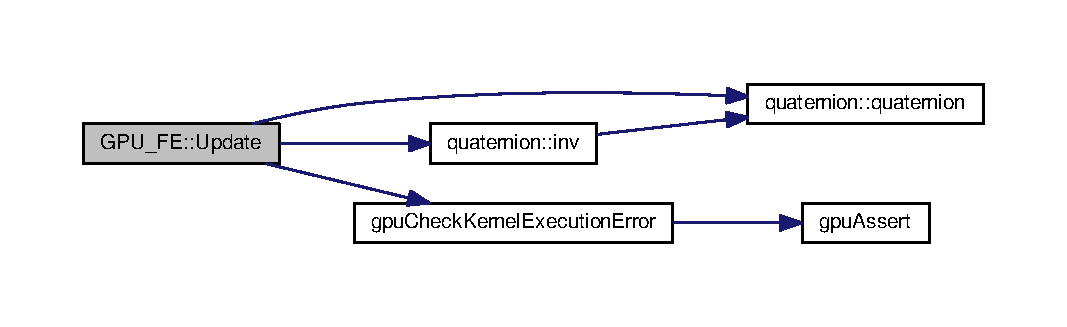
\includegraphics[width=350pt]{classGPU__FE_aa9039bd613961d4e0911b8514ed14fba_cgraph}
\end{center}
\end{figure}




\subsubsection{Member Data Documentation}
\index{G\+P\+U\+\_\+\+FE@{G\+P\+U\+\_\+\+FE}!C@{C}}
\index{C@{C}!G\+P\+U\+\_\+\+FE@{G\+P\+U\+\_\+\+FE}}
\paragraph[{\texorpdfstring{C}{C}}]{\setlength{\rightskip}{0pt plus 5cm}{\bf Cam}$\ast$ G\+P\+U\+\_\+\+F\+E\+::C\hspace{0.3cm}{\ttfamily [private]}}\hypertarget{classGPU__FE_aada926a7b999648bcb837507bf6a75d3}{}\label{classGPU__FE_aada926a7b999648bcb837507bf6a75d3}


Pointer ot \hyperlink{structCam}{Cam} struct stored on device. 



Definition at line \hyperlink{Voxel_8cuh_source_l00628}{628} of file \hyperlink{Voxel_8cuh_source}{Voxel.\+cuh}.

\index{G\+P\+U\+\_\+\+FE@{G\+P\+U\+\_\+\+FE}!D@{D}}
\index{D@{D}!G\+P\+U\+\_\+\+FE@{G\+P\+U\+\_\+\+FE}}
\paragraph[{\texorpdfstring{D}{D}}]{\setlength{\rightskip}{0pt plus 5cm}unsigned short$\ast$ G\+P\+U\+\_\+\+F\+E\+::D\hspace{0.3cm}{\ttfamily [private]}}\hypertarget{classGPU__FE_a20be80d2f552afc21f97831fcc4983e9}{}\label{classGPU__FE_a20be80d2f552afc21f97831fcc4983e9}


Pointer to depth image stored on device. 



Definition at line \hyperlink{Voxel_8cuh_source_l00624}{624} of file \hyperlink{Voxel_8cuh_source}{Voxel.\+cuh}.

\index{G\+P\+U\+\_\+\+FE@{G\+P\+U\+\_\+\+FE}!dtemp@{dtemp}}
\index{dtemp@{dtemp}!G\+P\+U\+\_\+\+FE@{G\+P\+U\+\_\+\+FE}}
\paragraph[{\texorpdfstring{dtemp}{dtemp}}]{\setlength{\rightskip}{0pt plus 5cm}{\bf Pair}$<$ long, {\bf Pair}$<${\bf voxel} $\ast$, {\bf Point}$>$ $>$$\ast$ G\+P\+U\+\_\+\+F\+E\+::dtemp\hspace{0.3cm}{\ttfamily [private]}}\hypertarget{classGPU__FE_a15cab1132ca16d50844a60cc09235567}{}\label{classGPU__FE_a15cab1132ca16d50844a60cc09235567}


Temporary array stored in device memory. 

This temporary array is used to store pointers to voxels created during current update on the device. \begin{DoxySeeAlso}{See also}
\hyperlink{Voxel_8cuh_a935fc0c42796b23607cf6f81a1e95e8d}{Update\+\_\+root} 
\end{DoxySeeAlso}


Definition at line \hyperlink{Voxel_8cuh_source_l00618}{618} of file \hyperlink{Voxel_8cuh_source}{Voxel.\+cuh}.

\index{G\+P\+U\+\_\+\+FE@{G\+P\+U\+\_\+\+FE}!htemp@{htemp}}
\index{htemp@{htemp}!G\+P\+U\+\_\+\+FE@{G\+P\+U\+\_\+\+FE}}
\paragraph[{\texorpdfstring{htemp}{htemp}}]{\setlength{\rightskip}{0pt plus 5cm}{\bf Pair}$<$ long, {\bf Pair}$<${\bf voxel} $\ast$, {\bf Point}$>$ $>$$\ast$ G\+P\+U\+\_\+\+F\+E\+::htemp\hspace{0.3cm}{\ttfamily [private]}}\hypertarget{classGPU__FE_afd39eabc36a87a6cde62b57296efcc8a}{}\label{classGPU__FE_afd39eabc36a87a6cde62b57296efcc8a}


Temporary array stored in host memory. 

This temporary array is used to copy the contents of dtemp vector and append them to HV vector. 

Definition at line \hyperlink{Voxel_8cuh_source_l00622}{622} of file \hyperlink{Voxel_8cuh_source}{Voxel.\+cuh}.

\index{G\+P\+U\+\_\+\+FE@{G\+P\+U\+\_\+\+FE}!HV@{HV}}
\index{HV@{HV}!G\+P\+U\+\_\+\+FE@{G\+P\+U\+\_\+\+FE}}
\paragraph[{\texorpdfstring{HV}{HV}}]{\setlength{\rightskip}{0pt plus 5cm}thrust\+::host\+\_\+vector$<$ {\bf Pair}$<$ long, {\bf Pair}$<${\bf voxel} $\ast$, {\bf Point}$>$ $>$ $>$ G\+P\+U\+\_\+\+F\+E\+::\+HV\hspace{0.3cm}{\ttfamily [private]}}\hypertarget{classGPU__FE_a7418d50e4e22db3671d9c000344aaddc}{}\label{classGPU__FE_a7418d50e4e22db3671d9c000344aaddc}


Vector in host memory containing root voxels. 

The vector is sorted using the index of the root voxels and is copied on to a device-\/side vector before passing to the kernel methods. 

Definition at line \hyperlink{Voxel_8cuh_source_l00611}{611} of file \hyperlink{Voxel_8cuh_source}{Voxel.\+cuh}.

\index{G\+P\+U\+\_\+\+FE@{G\+P\+U\+\_\+\+FE}!P@{P}}
\index{P@{P}!G\+P\+U\+\_\+\+FE@{G\+P\+U\+\_\+\+FE}}
\paragraph[{\texorpdfstring{P}{P}}]{\setlength{\rightskip}{0pt plus 5cm}{\bf Pose}$\ast$ G\+P\+U\+\_\+\+F\+E\+::P\hspace{0.3cm}{\ttfamily [private]}}\hypertarget{classGPU__FE_a1a99fc5bf3cc72c1d39f779e632f5fe7}{}\label{classGPU__FE_a1a99fc5bf3cc72c1d39f779e632f5fe7}


Pointer to \hyperlink{structPose}{Pose} struct stored on device. 



Definition at line \hyperlink{Voxel_8cuh_source_l00626}{626} of file \hyperlink{Voxel_8cuh_source}{Voxel.\+cuh}.

\index{G\+P\+U\+\_\+\+FE@{G\+P\+U\+\_\+\+FE}!s@{s}}
\index{s@{s}!G\+P\+U\+\_\+\+FE@{G\+P\+U\+\_\+\+FE}}
\paragraph[{\texorpdfstring{s}{s}}]{\setlength{\rightskip}{0pt plus 5cm}long G\+P\+U\+\_\+\+F\+E\+::s\hspace{0.3cm}{\ttfamily [private]}}\hypertarget{classGPU__FE_a0bd3424bf1e7775fc5eef2d17714cd94}{}\label{classGPU__FE_a0bd3424bf1e7775fc5eef2d17714cd94}


Size of HV vector. 



Definition at line \hyperlink{Voxel_8cuh_source_l00613}{613} of file \hyperlink{Voxel_8cuh_source}{Voxel.\+cuh}.

\index{G\+P\+U\+\_\+\+FE@{G\+P\+U\+\_\+\+FE}!S@{S}}
\index{S@{S}!G\+P\+U\+\_\+\+FE@{G\+P\+U\+\_\+\+FE}}
\paragraph[{\texorpdfstring{S}{S}}]{\setlength{\rightskip}{0pt plus 5cm}long$\ast$ G\+P\+U\+\_\+\+F\+E\+::S\hspace{0.3cm}{\ttfamily [private]}}\hypertarget{classGPU__FE_a1e2b5d0d82b739ab93b43e2bb862392a}{}\label{classGPU__FE_a1e2b5d0d82b739ab93b43e2bb862392a}


Size of HV vector; passed to device. 



Definition at line \hyperlink{Voxel_8cuh_source_l00630}{630} of file \hyperlink{Voxel_8cuh_source}{Voxel.\+cuh}.



The documentation for this class was generated from the following file\+:\begin{DoxyCompactItemize}
\item 
include/\hyperlink{Voxel_8cuh}{Voxel.\+cuh}\end{DoxyCompactItemize}

\hypertarget{classleaf}{}\subsection{leaf Class Reference}
\label{classleaf}\index{leaf@{leaf}}


Leaf nodes of the Octree structure.  




{\ttfamily \#include $<$Voxel.\+hpp$>$}

\subsubsection*{Public Member Functions}
\begin{DoxyCompactItemize}
\item 
\+\_\+\+\_\+device\+\_\+\+\_\+ \hyperlink{classleaf_adfaf04cd4b50545cbc902d1aa36bc609}{leaf} (float x, float y, float z)
\begin{DoxyCompactList}\small\item\em Constructor for leaf node. \end{DoxyCompactList}\item 
\+\_\+\+\_\+device\+\_\+\+\_\+ void \hyperlink{classleaf_a3c205ce57e242832977bde6e1a04d7da}{update\+\_\+leaf} (float x, float y, float z)
\begin{DoxyCompactList}\small\item\em Update method for this node object. \end{DoxyCompactList}\item 
\hyperlink{classleaf_aafe906fcbc78cef65683b3015de636bd}{leaf} (float x, float y, float z)
\begin{DoxyCompactList}\small\item\em Constructor for leaf node. \end{DoxyCompactList}\item 
void \hyperlink{classleaf_adacc1e0d36163c7fd0a7c31576ecf4e8}{update\+\_\+leaf} (float x, float y, float z)
\begin{DoxyCompactList}\small\item\em Update method for this node object. \end{DoxyCompactList}\end{DoxyCompactItemize}
\subsubsection*{Public Attributes}
\begin{DoxyCompactItemize}
\item 
float \hyperlink{classleaf_a4fc347dbd4f5911bbb477910588ed512}{\+\_\+v}
\begin{DoxyCompactList}\small\item\em Inverse of variance. \end{DoxyCompactList}\end{DoxyCompactItemize}
\begin{Indent}{\bf Co-\/ordinates}\par
{\em Co-\/ordinates of point inside leaf node divided by the variance.

The co-\/ordinates are measured relative to leaf node edge length, ie. $x, y, z \in [0,1)$. Note that although x\+\_\+v, y\+\_\+v, and z\+\_\+v can are unbounded, the values of x, y, and z are bounded since the update is a convex combination of two points inside the node. The co-\/ordinates are divided by the variance so that the update can be performed in a single atomic operation while running in G\+PU. \begin{DoxySeeAlso}{See also}
\hyperlink{Voxel_8cuh}{Voxel.\+cuh} 
\end{DoxySeeAlso}
}\begin{DoxyCompactItemize}
\item 
float \hyperlink{classleaf_ac34a93ca5739928d7389b12e735252d4}{x\+\_\+v}
\item 
float \hyperlink{classleaf_a06a94d40da44b846913db4d8900b2626}{y\+\_\+v}
\item 
float \hyperlink{classleaf_a5f51fe13eb6e53bd9549469011e7a10e}{z\+\_\+v}
\end{DoxyCompactItemize}
\end{Indent}


\subsubsection{Detailed Description}
Leaf nodes of the Octree structure. 

G\+PU\+: ~\newline
 This is not implemented as a voxel object because there can be millions of nodes and so the size should be as small as possible. Stores the x, y, z co-\/ordinates of a single point inside it relative to edge length ie. $x, y, z \in [0,1)$. This is to maintain uniform accuracy across all points. (accuracy of float type reduces as one moves away from 0) The origin of the node is the vertex with all co-\/ordinates minimum. ie. if the origin of voxel is $(x_o, y_o, z_o)$ and edge length is $L$, The vertices of the node are $\{(x_o, y_o, z_o), ..., (x_o+L, y_o+L, z_o+L)\}$ If the member \hyperlink{classleaf_a4fc347dbd4f5911bbb477910588ed512}{leaf\+::\+\_\+v} $> 0$, the leaf node is occupied. If \hyperlink{classleaf_a4fc347dbd4f5911bbb477910588ed512}{leaf\+::\+\_\+v} $= 0$, the leaf node is empty (this is not the same as unobserved. This means that this node has been observed, but there is no point inside it). This has been used becuase if initially a node was observed to be empty, and containing a point afterwards, the same update rule can be used without any change, in a single atomic operation. Although this is not particularly important for the C\+PU operation, it is extremely essential for the G\+PU operation to maintain consistency. An object of this class can only be declared inside the C\+U\+DA kernel.

C\+PU\+: ~\newline
 This is not implemented as a voxel object because there can be millions of nodes and so the size should be as small as possible. Stores the x, y, z co-\/ordinates of a single point inside it relative to edge length ie. $x, y, z \in [0,1)$. This is to maintain uniform accuracy across all points. (accuracy of float type reduces as one moves away from 0) The origin of the node is the vertex with all co-\/ordinates minimum. ie. if the origin of voxel is $(x_o, y_o, z_o)$ and edge length is $L$, The vertices of the node are $\{(x_o, y_o, z_o), ..., (x_o+L, y_o+L, z_o+L)\}$ If the member \hyperlink{classleaf_a4fc347dbd4f5911bbb477910588ed512}{leaf\+::\+\_\+v} $> 0$, the leaf node is occupied. If \hyperlink{classleaf_a4fc347dbd4f5911bbb477910588ed512}{leaf\+::\+\_\+v} $= 0$, the leaf node is empty (this is not the same as unobserved. This means that this node has been observed, but there is no point inside it). This has been used becuase if initially a node was observed to be empty, and containing a point afterwards, the same update rule can be used without any change, in a single atomic operation. Although this is not particularly important for the C\+PU operation, it is extremely essential for the G\+PU operation to maintain consistency. \begin{DoxySeeAlso}{See also}
\hyperlink{Voxel_8cuh}{Voxel.\+cuh} 
\end{DoxySeeAlso}


Definition at line \hyperlink{Voxel_8cuh_source_l00228}{228} of file \hyperlink{Voxel_8cuh_source}{Voxel.\+cuh}.



\subsubsection{Constructor \& Destructor Documentation}
\index{leaf@{leaf}!leaf@{leaf}}
\index{leaf@{leaf}!leaf@{leaf}}
\paragraph[{\texorpdfstring{leaf(float x, float y, float z)}{leaf(float x, float y, float z)}}]{\setlength{\rightskip}{0pt plus 5cm}\+\_\+\+\_\+device\+\_\+\+\_\+ leaf\+::leaf (
\begin{DoxyParamCaption}
\item[{float}]{x, }
\item[{float}]{y, }
\item[{float}]{z}
\end{DoxyParamCaption}
)\hspace{0.3cm}{\ttfamily [inline]}}\hypertarget{classleaf_adfaf04cd4b50545cbc902d1aa36bc609}{}\label{classleaf_adfaf04cd4b50545cbc902d1aa36bc609}


Constructor for leaf node. 

Note that this is the only constructor provided. 
\begin{DoxyParams}{Parameters}
{\em (x,y,z)} & relative to leaf node, ie. $x, y, z \in [0,1)$ for correct operation \\
\hline
\end{DoxyParams}


Definition at line \hyperlink{Voxel_8cuh_source_l00257}{257} of file \hyperlink{Voxel_8cuh_source}{Voxel.\+cuh}.

\index{leaf@{leaf}!leaf@{leaf}}
\index{leaf@{leaf}!leaf@{leaf}}
\paragraph[{\texorpdfstring{leaf(float x, float y, float z)}{leaf(float x, float y, float z)}}]{\setlength{\rightskip}{0pt plus 5cm}leaf\+::leaf (
\begin{DoxyParamCaption}
\item[{float}]{x, }
\item[{float}]{y, }
\item[{float}]{z}
\end{DoxyParamCaption}
)\hspace{0.3cm}{\ttfamily [inline]}}\hypertarget{classleaf_aafe906fcbc78cef65683b3015de636bd}{}\label{classleaf_aafe906fcbc78cef65683b3015de636bd}


Constructor for leaf node. 

Note that this is the only constructor provided. If the parameters provided are $(-1, -1, -,1)$, the node is set to be empty. Note that x\+\_\+v, y\+\_\+v, and z\+\_\+v are set $= 0$. 
\begin{DoxyParams}{Parameters}
{\em (x,y,z)} & relative to leaf node, ie. $x, y, z \in [0,1)$ for correct operation \\
\hline
\end{DoxyParams}


Definition at line \hyperlink{Voxel_8hpp_source_l00155}{155} of file \hyperlink{Voxel_8hpp_source}{Voxel.\+hpp}.



\subsubsection{Member Function Documentation}
\index{leaf@{leaf}!update\+\_\+leaf@{update\+\_\+leaf}}
\index{update\+\_\+leaf@{update\+\_\+leaf}!leaf@{leaf}}
\paragraph[{\texorpdfstring{update\+\_\+leaf(float x, float y, float z)}{update_leaf(float x, float y, float z)}}]{\setlength{\rightskip}{0pt plus 5cm}void leaf\+::update\+\_\+leaf (
\begin{DoxyParamCaption}
\item[{float}]{x, }
\item[{float}]{y, }
\item[{float}]{z}
\end{DoxyParamCaption}
)\hspace{0.3cm}{\ttfamily [inline]}}\hypertarget{classleaf_adacc1e0d36163c7fd0a7c31576ecf4e8}{}\label{classleaf_adacc1e0d36163c7fd0a7c31576ecf4e8}


Update method for this node object. 

Since every node contains only a single point, this update rule is used to combine the points into a single point. This is the same as the Measurement Update Step in E\+KF and S\+L\+AM. In this particular case the rule is a simple weighted average. So, if the point already existing in the node has a very low variance, the updated point will be very close to the previous point. Even if an anisotropic gaussian probability distribution function is used, the updated point will always be a convex combination of two points. 
\begin{DoxyParams}{Parameters}
{\em (x,y,z)} & relative to leaf node, ie. $x, y, z \in [0,1)$ for correct operation \\
\hline
\end{DoxyParams}


Definition at line \hyperlink{Voxel_8hpp_source_l00169}{169} of file \hyperlink{Voxel_8hpp_source}{Voxel.\+hpp}.

\index{leaf@{leaf}!update\+\_\+leaf@{update\+\_\+leaf}}
\index{update\+\_\+leaf@{update\+\_\+leaf}!leaf@{leaf}}
\paragraph[{\texorpdfstring{update\+\_\+leaf(float x, float y, float z)}{update_leaf(float x, float y, float z)}}]{\setlength{\rightskip}{0pt plus 5cm}\+\_\+\+\_\+device\+\_\+\+\_\+ void leaf\+::update\+\_\+leaf (
\begin{DoxyParamCaption}
\item[{float}]{x, }
\item[{float}]{y, }
\item[{float}]{z}
\end{DoxyParamCaption}
)\hspace{0.3cm}{\ttfamily [inline]}}\hypertarget{classleaf_a3c205ce57e242832977bde6e1a04d7da}{}\label{classleaf_a3c205ce57e242832977bde6e1a04d7da}


Update method for this node object. 

Since every node contains only a single point, this update rule is used to combine the points into a single point. This is the same as the Measurement Update Step in E\+KF and S\+L\+AM. In this particular case the rule is a simple weighted average. So, if the point already existing in the node has a very low variance, the updated point will be very close to the previous point. Even if an anisotropic gaussian probability distribution function is used, the updated point will always be a convex combination of two points. atommic\+Add() function and the transformed variables ensure consistency while multi-\/threading. 
\begin{DoxyParams}{Parameters}
{\em (x,y,z)} & relative to leaf node, ie. $x, y, z \in [0,1)$ for correct operation \\
\hline
\end{DoxyParams}


Definition at line \hyperlink{Voxel_8cuh_source_l00270}{270} of file \hyperlink{Voxel_8cuh_source}{Voxel.\+cuh}.



Here is the caller graph for this function\+:\nopagebreak
\begin{figure}[H]
\begin{center}
\leavevmode
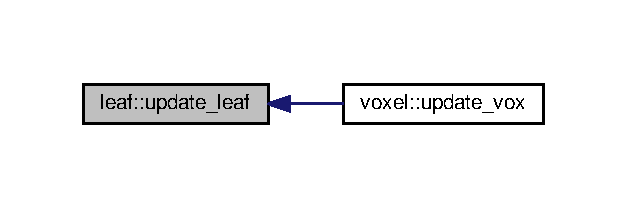
\includegraphics[width=301pt]{classleaf_a3c205ce57e242832977bde6e1a04d7da_icgraph}
\end{center}
\end{figure}




\subsubsection{Member Data Documentation}
\index{leaf@{leaf}!\+\_\+v@{\+\_\+v}}
\index{\+\_\+v@{\+\_\+v}!leaf@{leaf}}
\paragraph[{\texorpdfstring{\+\_\+v}{_v}}]{\setlength{\rightskip}{0pt plus 5cm}float leaf\+::\+\_\+v}\hypertarget{classleaf_a4fc347dbd4f5911bbb477910588ed512}{}\label{classleaf_a4fc347dbd4f5911bbb477910588ed512}


Inverse of variance. 

The points are assumed to be distributed as a 3-\/D uniform gaussian distribution when measured. As more points are updated in the node, this variance decreases, ie. the certainity of a point existing in the node increases. The update rule is the typical update rule of gaussian distribution, same as the one in Measurement Update Step in E\+KF and S\+L\+AM. Inverse of variance is stored so that the update can be performed in a single atomic step while running in G\+PU. \begin{DoxySeeAlso}{See also}
\hyperlink{Voxel_8cuh}{Voxel.\+cuh} 
\end{DoxySeeAlso}


Definition at line \hyperlink{Voxel_8cuh_source_l00239}{239} of file \hyperlink{Voxel_8cuh_source}{Voxel.\+cuh}.

\index{leaf@{leaf}!x\+\_\+v@{x\+\_\+v}}
\index{x\+\_\+v@{x\+\_\+v}!leaf@{leaf}}
\paragraph[{\texorpdfstring{x\+\_\+v}{x_v}}]{\setlength{\rightskip}{0pt plus 5cm}float leaf\+::x\+\_\+v}\hypertarget{classleaf_ac34a93ca5739928d7389b12e735252d4}{}\label{classleaf_ac34a93ca5739928d7389b12e735252d4}


Definition at line \hyperlink{Voxel_8cuh_source_l00250}{250} of file \hyperlink{Voxel_8cuh_source}{Voxel.\+cuh}.

\index{leaf@{leaf}!y\+\_\+v@{y\+\_\+v}}
\index{y\+\_\+v@{y\+\_\+v}!leaf@{leaf}}
\paragraph[{\texorpdfstring{y\+\_\+v}{y_v}}]{\setlength{\rightskip}{0pt plus 5cm}float leaf\+::y\+\_\+v}\hypertarget{classleaf_a06a94d40da44b846913db4d8900b2626}{}\label{classleaf_a06a94d40da44b846913db4d8900b2626}


Definition at line \hyperlink{Voxel_8cuh_source_l00250}{250} of file \hyperlink{Voxel_8cuh_source}{Voxel.\+cuh}.

\index{leaf@{leaf}!z\+\_\+v@{z\+\_\+v}}
\index{z\+\_\+v@{z\+\_\+v}!leaf@{leaf}}
\paragraph[{\texorpdfstring{z\+\_\+v}{z_v}}]{\setlength{\rightskip}{0pt plus 5cm}float leaf\+::z\+\_\+v}\hypertarget{classleaf_a5f51fe13eb6e53bd9549469011e7a10e}{}\label{classleaf_a5f51fe13eb6e53bd9549469011e7a10e}


Definition at line \hyperlink{Voxel_8cuh_source_l00250}{250} of file \hyperlink{Voxel_8cuh_source}{Voxel.\+cuh}.



The documentation for this class was generated from the following files\+:\begin{DoxyCompactItemize}
\item 
include/\hyperlink{Voxel_8cuh}{Voxel.\+cuh}\item 
include/\hyperlink{Voxel_8hpp}{Voxel.\+hpp}\end{DoxyCompactItemize}

\hypertarget{classLogger}{}\subsection{Logger Class Reference}
\label{classLogger}\index{Logger@{Logger}}


Logging class.  




{\ttfamily \#include $<$Logging.\+hpp$>$}



Collaboration diagram for Logger\+:\nopagebreak
\begin{figure}[H]
\begin{center}
\leavevmode
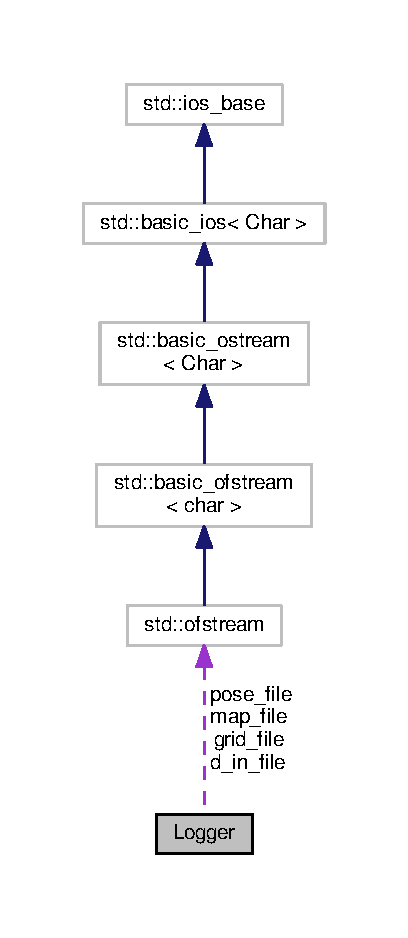
\includegraphics[width=196pt]{classLogger__coll__graph}
\end{center}
\end{figure}
\subsubsection*{Public Member Functions}
\begin{DoxyCompactItemize}
\item 
\hyperlink{classLogger_abc41bfb031d896170c7675fa96a6b30c}{Logger} ()
\begin{DoxyCompactList}\small\item\em Default Constructor. \end{DoxyCompactList}\item 
void \hyperlink{classLogger_a42c282f4c0e2c6557d16e2967c1ddf7e}{Init} ()
\begin{DoxyCompactList}\small\item\em Initializes \hyperlink{classLogger}{Logger}. \end{DoxyCompactList}\item 
void \hyperlink{classLogger_adcc95257ff2edceded8e272dac3603ce}{Log} (\hyperlink{classCamera}{Camera} const $\ast$C, rs2\+\_\+pose const $\ast$pose, cv\+::\+Mat const $\ast$depth)
\begin{DoxyCompactList}\small\item\em Real-\/time logging method. \end{DoxyCompactList}\item 
void \hyperlink{classLogger_a6b670ceb54a249eb83da08a1914d2be8}{Close} (\hyperlink{classCamera}{Camera} const $\ast$C, \hyperlink{classMap__FE}{Map\+\_\+\+FE} $\ast$F)
\begin{DoxyCompactList}\small\item\em Closes the lgging operation. \end{DoxyCompactList}\end{DoxyCompactItemize}
\subsubsection*{Private Member Functions}
\begin{DoxyCompactItemize}
\item 
void \hyperlink{classLogger_ac58fee4bd66a5359deb29a86948d584d}{obj\+\_\+grid} (\hyperlink{classMap__FE}{Map\+\_\+\+FE} $\ast$F)
\begin{DoxyCompactList}\small\item\em Constructs a grid representation of the map. \end{DoxyCompactList}\item 
void \hyperlink{classLogger_a38c5de03e0de7deffd7b516b13f826ff}{point\+\_\+grid} (float x, float y, float z, float m\+\_\+x, float m\+\_\+y, float m\+\_\+z, float size)
\begin{DoxyCompactList}\small\item\em Recursively constructs a voxel wireframe. \end{DoxyCompactList}\end{DoxyCompactItemize}
\subsubsection*{Private Attributes}
\begin{DoxyCompactItemize}
\item 
bool \hyperlink{classLogger_a99c616f02a46e95f2e976ab7d880dbc5}{start}
\begin{DoxyCompactList}\small\item\em Boolean value to keep track of Logging execution. \end{DoxyCompactList}\item 
std\+::chrono\+::high\+\_\+resolution\+\_\+clock\+::time\+\_\+point \hyperlink{classLogger_a7f6f65922677036ca61ba12a19fdb719}{ti}
\begin{DoxyCompactList}\small\item\em High-\/resolution clock to record timestamps of relevant data. \end{DoxyCompactList}\item 
time\+\_\+t \hyperlink{classLogger_afe5c4b612d69878aa65ce940a042fd8c}{today}
\begin{DoxyCompactList}\small\item\em Time at logging initiation. \end{DoxyCompactList}\item 
char \hyperlink{classLogger_a0fd4efa39e08c0253f59f76e08abefee}{buf} \mbox{[}80\mbox{]}
\begin{DoxyCompactList}\small\item\em Character array to store today. \end{DoxyCompactList}\item 
Gnuplot \hyperlink{classLogger_a63eca256c57dee44717f3002654887c7}{gp}
\begin{DoxyCompactList}\small\item\em Gnuplot instance. \end{DoxyCompactList}\end{DoxyCompactItemize}
{\bf }\par
\begin{DoxyCompactItemize}
\item 
std\+::ofstream \hyperlink{classLogger_a7314c685ce4579a7d8b118e5d5327d13}{pose\+\_\+file}
\begin{DoxyCompactList}\small\item\em \hyperlink{structPose}{Pose} log file. \end{DoxyCompactList}\item 
std\+::ofstream \hyperlink{classLogger_acf9b6a89a6f8c520d010d87cff33b9df}{d\+\_\+in\+\_\+file}
\begin{DoxyCompactList}\small\item\em Depth intrinsics file. \end{DoxyCompactList}\item 
cv\+::\+Video\+Writer \hyperlink{classLogger_a5e5b9ad704575bda69b184a5b136735f}{depth\+\_\+file}
\begin{DoxyCompactList}\small\item\em Depth feed video file. \end{DoxyCompactList}\item 
std\+::ofstream \hyperlink{classLogger_a1aedce7141d1346bc39c94e3a3eba4d6}{map\+\_\+file}
\begin{DoxyCompactList}\small\item\em Global map file. \end{DoxyCompactList}\item 
std\+::ofstream \hyperlink{classLogger_a715ae637741f3b00ba8ebb9858cb5577}{grid\+\_\+file}
\begin{DoxyCompactList}\small\item\em Grid file. \end{DoxyCompactList}\end{DoxyCompactItemize}



\subsubsection{Detailed Description}
Logging class. 

Instance of this class can be used to log information from the cameras and the global map. Logging can happen either in real-\/time or after program termination. Real-\/time logging can cause performance issues, and should be used only for debugging purposes. Correct termination of the program should be ensured in order to avoid inconsistent logged data. 

Definition at line \hyperlink{Logging_8hpp_source_l00052}{52} of file \hyperlink{Logging_8hpp_source}{Logging.\+hpp}.



\subsubsection{Constructor \& Destructor Documentation}
\index{Logger@{Logger}!Logger@{Logger}}
\index{Logger@{Logger}!Logger@{Logger}}
\paragraph[{\texorpdfstring{Logger()}{Logger()}}]{\setlength{\rightskip}{0pt plus 5cm}Logger\+::\+Logger (
\begin{DoxyParamCaption}
{}
\end{DoxyParamCaption}
)\hspace{0.3cm}{\ttfamily [inline]}}\hypertarget{classLogger_abc41bfb031d896170c7675fa96a6b30c}{}\label{classLogger_abc41bfb031d896170c7675fa96a6b30c}


Default Constructor. 

Current day and time are stored into the buf char array. 

Definition at line \hyperlink{Logging_8hpp_source_l00091}{91} of file \hyperlink{Logging_8hpp_source}{Logging.\+hpp}.



\subsubsection{Member Function Documentation}
\index{Logger@{Logger}!Close@{Close}}
\index{Close@{Close}!Logger@{Logger}}
\paragraph[{\texorpdfstring{Close(\+Camera const $\ast$\+C, Map\+\_\+\+F\+E $\ast$\+F)}{Close(Camera const *C, Map_FE *F)}}]{\setlength{\rightskip}{0pt plus 5cm}void Logger\+::\+Close (
\begin{DoxyParamCaption}
\item[{{\bf Camera} const $\ast$}]{C, }
\item[{{\bf Map\+\_\+\+FE} $\ast$}]{F}
\end{DoxyParamCaption}
)\hspace{0.3cm}{\ttfamily [inline]}}\hypertarget{classLogger_a6b670ceb54a249eb83da08a1914d2be8}{}\label{classLogger_a6b670ceb54a249eb83da08a1914d2be8}


Closes the lgging operation. 

All non real-\/time logging is done in this method. It also closes the files in memory so that they can accessed later. Since a pointer to \hyperlink{classMap__FE}{Map\+\_\+\+FE} object is taken as input, any valid map implementation, inherited from \hyperlink{classMap__FE}{Map\+\_\+\+FE} will be consistent with the method. 
\begin{DoxyParams}{Parameters}
{\em Camea} & object \\
\hline
{\em \hyperlink{classMap__FE}{Map\+\_\+\+FE}} & pointer \\
\hline
\end{DoxyParams}


Definition at line \hyperlink{Logging_8hpp_source_l00192}{192} of file \hyperlink{Logging_8hpp_source}{Logging.\+hpp}.



Here is the call graph for this function\+:\nopagebreak
\begin{figure}[H]
\begin{center}
\leavevmode
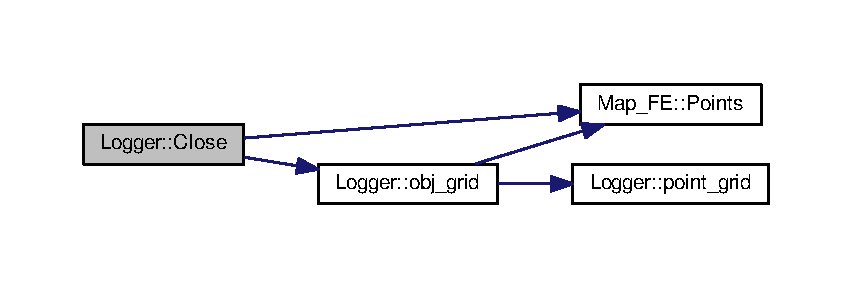
\includegraphics[width=350pt]{classLogger_a6b670ceb54a249eb83da08a1914d2be8_cgraph}
\end{center}
\end{figure}




Here is the caller graph for this function\+:\nopagebreak
\begin{figure}[H]
\begin{center}
\leavevmode
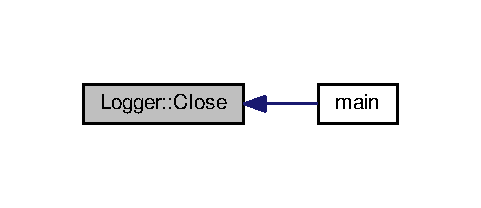
\includegraphics[width=231pt]{classLogger_a6b670ceb54a249eb83da08a1914d2be8_icgraph}
\end{center}
\end{figure}


\index{Logger@{Logger}!Init@{Init}}
\index{Init@{Init}!Logger@{Logger}}
\paragraph[{\texorpdfstring{Init()}{Init()}}]{\setlength{\rightskip}{0pt plus 5cm}void Logger\+::\+Init (
\begin{DoxyParamCaption}
{}
\end{DoxyParamCaption}
)\hspace{0.3cm}{\ttfamily [inline]}}\hypertarget{classLogger_a42c282f4c0e2c6557d16e2967c1ddf7e}{}\label{classLogger_a42c282f4c0e2c6557d16e2967c1ddf7e}


Initializes \hyperlink{classLogger}{Logger}. 

The output files are memory mapped and opened with the corresponding file names. 

Definition at line \hyperlink{Logging_8hpp_source_l00100}{100} of file \hyperlink{Logging_8hpp_source}{Logging.\+hpp}.



Here is the caller graph for this function\+:\nopagebreak
\begin{figure}[H]
\begin{center}
\leavevmode
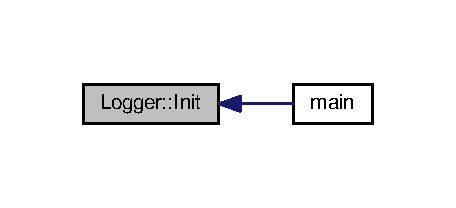
\includegraphics[width=219pt]{classLogger_a42c282f4c0e2c6557d16e2967c1ddf7e_icgraph}
\end{center}
\end{figure}


\index{Logger@{Logger}!Log@{Log}}
\index{Log@{Log}!Logger@{Logger}}
\paragraph[{\texorpdfstring{Log(\+Camera const $\ast$\+C, rs2\+\_\+pose const $\ast$pose, cv\+::\+Mat const $\ast$depth)}{Log(Camera const *C, rs2_pose const *pose, cv::Mat const *depth)}}]{\setlength{\rightskip}{0pt plus 5cm}void Logger\+::\+Log (
\begin{DoxyParamCaption}
\item[{{\bf Camera} const $\ast$}]{C, }
\item[{rs2\+\_\+pose const $\ast$}]{pose, }
\item[{cv\+::\+Mat const $\ast$}]{depth}
\end{DoxyParamCaption}
)\hspace{0.3cm}{\ttfamily [inline]}}\hypertarget{classLogger_adcc95257ff2edceded8e272dac3603ce}{}\label{classLogger_adcc95257ff2edceded8e272dac3603ce}


Real-\/time logging method. 

All real-\/time logging and display are done in this method. Operations like display video feed or 3-\/D display can limit performance. But, it is recommended that pose logging is always set. 
\begin{DoxyParams}{Parameters}
{\em \hyperlink{classCamera}{Camera}} & object \\
\hline
{\em \hyperlink{structPose}{Pose}} & from T265 \\
\hline
{\em 16-\/bit} & depth image from D435 \\
\hline
\end{DoxyParams}


Definition at line \hyperlink{Logging_8hpp_source_l00121}{121} of file \hyperlink{Logging_8hpp_source}{Logging.\+hpp}.



Here is the caller graph for this function\+:\nopagebreak
\begin{figure}[H]
\begin{center}
\leavevmode
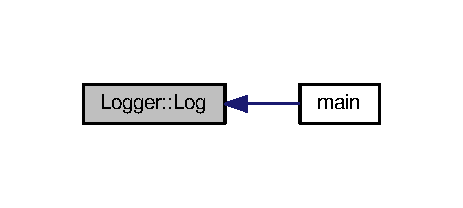
\includegraphics[width=222pt]{classLogger_adcc95257ff2edceded8e272dac3603ce_icgraph}
\end{center}
\end{figure}


\index{Logger@{Logger}!obj\+\_\+grid@{obj\+\_\+grid}}
\index{obj\+\_\+grid@{obj\+\_\+grid}!Logger@{Logger}}
\paragraph[{\texorpdfstring{obj\+\_\+grid(\+Map\+\_\+\+F\+E $\ast$\+F)}{obj_grid(Map_FE *F)}}]{\setlength{\rightskip}{0pt plus 5cm}void Logger\+::obj\+\_\+grid (
\begin{DoxyParamCaption}
\item[{{\bf Map\+\_\+\+FE} $\ast$}]{F}
\end{DoxyParamCaption}
)\hspace{0.3cm}{\ttfamily [inline]}, {\ttfamily [private]}}\hypertarget{classLogger_ac58fee4bd66a5359deb29a86948d584d}{}\label{classLogger_ac58fee4bd66a5359deb29a86948d584d}


Constructs a grid representation of the map. 

This method creates a gnuplot file, which can run using cmd \textquotesingle{}gnuplot $<$file-\/name$>$\textquotesingle{}. \hyperlink{classLogger_a38c5de03e0de7deffd7b516b13f826ff}{Logger\+::point\+\_\+grid()} is called on each of the leaf node points, which are aquired by \hyperlink{classMap__FE_aedfee41631a7287c9eb377ccb05317d6}{Map\+\_\+\+F\+E\+::\+Points()}. Called by \hyperlink{classLogger_a6b670ceb54a249eb83da08a1914d2be8}{Logger\+::\+Close()} 
\begin{DoxyParams}{Parameters}
{\em \hyperlink{classMap__FE}{Map\+\_\+\+FE}} & pointer \\
\hline
\end{DoxyParams}
\begin{DoxySeeAlso}{See also}
\hyperlink{classLogger_a6b670ceb54a249eb83da08a1914d2be8}{Logger\+::\+Close()}, \hyperlink{classLogger_a38c5de03e0de7deffd7b516b13f826ff}{Logger\+::point\+\_\+grid()}, \hyperlink{classMap__FE_aedfee41631a7287c9eb377ccb05317d6}{Map\+\_\+\+F\+E\+::\+Points()} 
\end{DoxySeeAlso}


Definition at line \hyperlink{Logging_8hpp_source_l00229}{229} of file \hyperlink{Logging_8hpp_source}{Logging.\+hpp}.



Here is the call graph for this function\+:\nopagebreak
\begin{figure}[H]
\begin{center}
\leavevmode
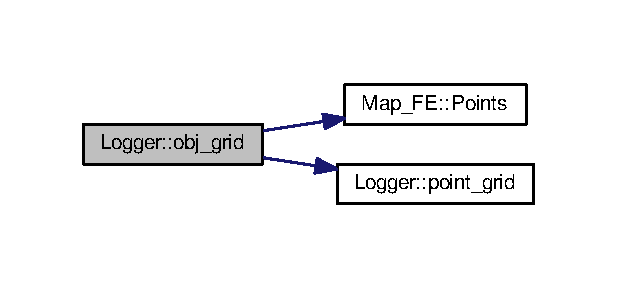
\includegraphics[width=296pt]{classLogger_ac58fee4bd66a5359deb29a86948d584d_cgraph}
\end{center}
\end{figure}




Here is the caller graph for this function\+:\nopagebreak
\begin{figure}[H]
\begin{center}
\leavevmode
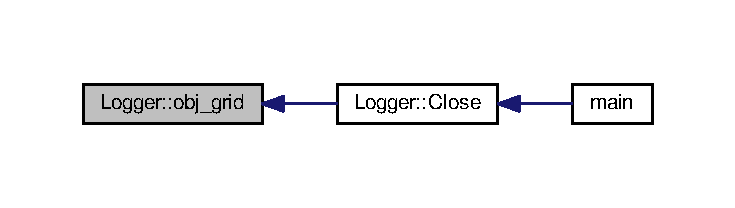
\includegraphics[width=350pt]{classLogger_ac58fee4bd66a5359deb29a86948d584d_icgraph}
\end{center}
\end{figure}


\index{Logger@{Logger}!point\+\_\+grid@{point\+\_\+grid}}
\index{point\+\_\+grid@{point\+\_\+grid}!Logger@{Logger}}
\paragraph[{\texorpdfstring{point\+\_\+grid(float x, float y, float z, float m\+\_\+x, float m\+\_\+y, float m\+\_\+z, float size)}{point_grid(float x, float y, float z, float m_x, float m_y, float m_z, float size)}}]{\setlength{\rightskip}{0pt plus 5cm}void Logger\+::point\+\_\+grid (
\begin{DoxyParamCaption}
\item[{float}]{x, }
\item[{float}]{y, }
\item[{float}]{z, }
\item[{float}]{m\+\_\+x, }
\item[{float}]{m\+\_\+y, }
\item[{float}]{m\+\_\+z, }
\item[{float}]{size}
\end{DoxyParamCaption}
)\hspace{0.3cm}{\ttfamily [inline]}, {\ttfamily [private]}}\hypertarget{classLogger_a38c5de03e0de7deffd7b516b13f826ff}{}\label{classLogger_a38c5de03e0de7deffd7b516b13f826ff}


Recursively constructs a voxel wireframe. 

This method constructs a wireframe around a voxel at each level of the octree. This is recursive method. 
\begin{DoxyParams}{Parameters}
{\em Co-\/ordinate} & of the origin of this voxel \\
\hline
{\em Co-\/ordinate} & of the point with respect to the voxel \\
\hline
{\em Size} & of the voxel at the current level \\
\hline
\end{DoxyParams}
\begin{DoxySeeAlso}{See also}
\hyperlink{classLogger_ac58fee4bd66a5359deb29a86948d584d}{Logger\+::obj\+\_\+grid()} 
\end{DoxySeeAlso}


Definition at line \hyperlink{Logging_8hpp_source_l00260}{260} of file \hyperlink{Logging_8hpp_source}{Logging.\+hpp}.



Here is the caller graph for this function\+:\nopagebreak
\begin{figure}[H]
\begin{center}
\leavevmode
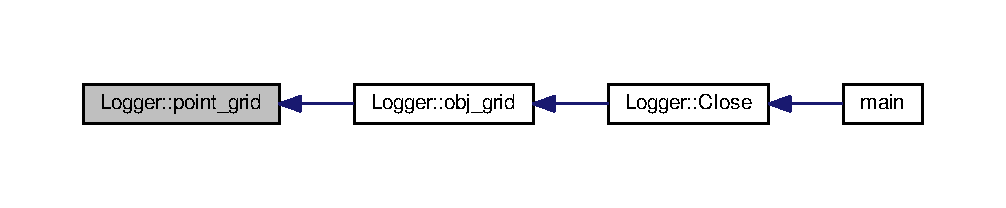
\includegraphics[width=350pt]{classLogger_a38c5de03e0de7deffd7b516b13f826ff_icgraph}
\end{center}
\end{figure}




\subsubsection{Member Data Documentation}
\index{Logger@{Logger}!buf@{buf}}
\index{buf@{buf}!Logger@{Logger}}
\paragraph[{\texorpdfstring{buf}{buf}}]{\setlength{\rightskip}{0pt plus 5cm}char Logger\+::buf\mbox{[}80\mbox{]}\hspace{0.3cm}{\ttfamily [private]}}\hypertarget{classLogger_a0fd4efa39e08c0253f59f76e08abefee}{}\label{classLogger_a0fd4efa39e08c0253f59f76e08abefee}


Character array to store today. 



Definition at line \hyperlink{Logging_8hpp_source_l00065}{65} of file \hyperlink{Logging_8hpp_source}{Logging.\+hpp}.

\index{Logger@{Logger}!d\+\_\+in\+\_\+file@{d\+\_\+in\+\_\+file}}
\index{d\+\_\+in\+\_\+file@{d\+\_\+in\+\_\+file}!Logger@{Logger}}
\paragraph[{\texorpdfstring{d\+\_\+in\+\_\+file}{d_in_file}}]{\setlength{\rightskip}{0pt plus 5cm}std\+::ofstream Logger\+::d\+\_\+in\+\_\+file\hspace{0.3cm}{\ttfamily [private]}}\hypertarget{classLogger_acf9b6a89a6f8c520d010d87cff33b9df}{}\label{classLogger_acf9b6a89a6f8c520d010d87cff33b9df}


Depth intrinsics file. 



Definition at line \hyperlink{Logging_8hpp_source_l00074}{74} of file \hyperlink{Logging_8hpp_source}{Logging.\+hpp}.

\index{Logger@{Logger}!depth\+\_\+file@{depth\+\_\+file}}
\index{depth\+\_\+file@{depth\+\_\+file}!Logger@{Logger}}
\paragraph[{\texorpdfstring{depth\+\_\+file}{depth_file}}]{\setlength{\rightskip}{0pt plus 5cm}cv\+::\+Video\+Writer Logger\+::depth\+\_\+file\hspace{0.3cm}{\ttfamily [private]}}\hypertarget{classLogger_a5e5b9ad704575bda69b184a5b136735f}{}\label{classLogger_a5e5b9ad704575bda69b184a5b136735f}


Depth feed video file. 



Definition at line \hyperlink{Logging_8hpp_source_l00076}{76} of file \hyperlink{Logging_8hpp_source}{Logging.\+hpp}.

\index{Logger@{Logger}!gp@{gp}}
\index{gp@{gp}!Logger@{Logger}}
\paragraph[{\texorpdfstring{gp}{gp}}]{\setlength{\rightskip}{0pt plus 5cm}Gnuplot Logger\+::gp\hspace{0.3cm}{\ttfamily [private]}}\hypertarget{classLogger_a63eca256c57dee44717f3002654887c7}{}\label{classLogger_a63eca256c57dee44717f3002654887c7}


Gnuplot instance. 



Definition at line \hyperlink{Logging_8hpp_source_l00084}{84} of file \hyperlink{Logging_8hpp_source}{Logging.\+hpp}.

\index{Logger@{Logger}!grid\+\_\+file@{grid\+\_\+file}}
\index{grid\+\_\+file@{grid\+\_\+file}!Logger@{Logger}}
\paragraph[{\texorpdfstring{grid\+\_\+file}{grid_file}}]{\setlength{\rightskip}{0pt plus 5cm}std\+::ofstream Logger\+::grid\+\_\+file\hspace{0.3cm}{\ttfamily [private]}}\hypertarget{classLogger_a715ae637741f3b00ba8ebb9858cb5577}{}\label{classLogger_a715ae637741f3b00ba8ebb9858cb5577}


Grid file. 



Definition at line \hyperlink{Logging_8hpp_source_l00080}{80} of file \hyperlink{Logging_8hpp_source}{Logging.\+hpp}.

\index{Logger@{Logger}!map\+\_\+file@{map\+\_\+file}}
\index{map\+\_\+file@{map\+\_\+file}!Logger@{Logger}}
\paragraph[{\texorpdfstring{map\+\_\+file}{map_file}}]{\setlength{\rightskip}{0pt plus 5cm}std\+::ofstream Logger\+::map\+\_\+file\hspace{0.3cm}{\ttfamily [private]}}\hypertarget{classLogger_a1aedce7141d1346bc39c94e3a3eba4d6}{}\label{classLogger_a1aedce7141d1346bc39c94e3a3eba4d6}


Global map file. 



Definition at line \hyperlink{Logging_8hpp_source_l00078}{78} of file \hyperlink{Logging_8hpp_source}{Logging.\+hpp}.

\index{Logger@{Logger}!pose\+\_\+file@{pose\+\_\+file}}
\index{pose\+\_\+file@{pose\+\_\+file}!Logger@{Logger}}
\paragraph[{\texorpdfstring{pose\+\_\+file}{pose_file}}]{\setlength{\rightskip}{0pt plus 5cm}std\+::ofstream Logger\+::pose\+\_\+file\hspace{0.3cm}{\ttfamily [private]}}\hypertarget{classLogger_a7314c685ce4579a7d8b118e5d5327d13}{}\label{classLogger_a7314c685ce4579a7d8b118e5d5327d13}


\hyperlink{structPose}{Pose} log file. 

Output log files 

Definition at line \hyperlink{Logging_8hpp_source_l00072}{72} of file \hyperlink{Logging_8hpp_source}{Logging.\+hpp}.

\index{Logger@{Logger}!start@{start}}
\index{start@{start}!Logger@{Logger}}
\paragraph[{\texorpdfstring{start}{start}}]{\setlength{\rightskip}{0pt plus 5cm}bool Logger\+::start\hspace{0.3cm}{\ttfamily [private]}}\hypertarget{classLogger_a99c616f02a46e95f2e976ab7d880dbc5}{}\label{classLogger_a99c616f02a46e95f2e976ab7d880dbc5}


Boolean value to keep track of Logging execution. 



Definition at line \hyperlink{Logging_8hpp_source_l00057}{57} of file \hyperlink{Logging_8hpp_source}{Logging.\+hpp}.

\index{Logger@{Logger}!ti@{ti}}
\index{ti@{ti}!Logger@{Logger}}
\paragraph[{\texorpdfstring{ti}{ti}}]{\setlength{\rightskip}{0pt plus 5cm}std\+::chrono\+::high\+\_\+resolution\+\_\+clock\+::time\+\_\+point Logger\+::ti\hspace{0.3cm}{\ttfamily [private]}}\hypertarget{classLogger_a7f6f65922677036ca61ba12a19fdb719}{}\label{classLogger_a7f6f65922677036ca61ba12a19fdb719}


High-\/resolution clock to record timestamps of relevant data. 



Definition at line \hyperlink{Logging_8hpp_source_l00060}{60} of file \hyperlink{Logging_8hpp_source}{Logging.\+hpp}.

\index{Logger@{Logger}!today@{today}}
\index{today@{today}!Logger@{Logger}}
\paragraph[{\texorpdfstring{today}{today}}]{\setlength{\rightskip}{0pt plus 5cm}time\+\_\+t Logger\+::today\hspace{0.3cm}{\ttfamily [private]}}\hypertarget{classLogger_afe5c4b612d69878aa65ce940a042fd8c}{}\label{classLogger_afe5c4b612d69878aa65ce940a042fd8c}


Time at logging initiation. 



Definition at line \hyperlink{Logging_8hpp_source_l00063}{63} of file \hyperlink{Logging_8hpp_source}{Logging.\+hpp}.



The documentation for this class was generated from the following file\+:\begin{DoxyCompactItemize}
\item 
include/\hyperlink{Logging_8hpp}{Logging.\+hpp}\end{DoxyCompactItemize}

\hypertarget{classMap__FE}{}\subsection{Map\+\_\+\+FE Class Reference}
\label{classMap__FE}\index{Map\+\_\+\+FE@{Map\+\_\+\+FE}}


Virtual class Parent of \hyperlink{classCPU__FE}{C\+P\+U\+\_\+\+FE} and \hyperlink{classGPU__FE}{G\+P\+U\+\_\+\+FE} classes.  




{\ttfamily \#include $<$Helper.\+hpp$>$}



Inheritance diagram for Map\+\_\+\+FE\+:\nopagebreak
\begin{figure}[H]
\begin{center}
\leavevmode
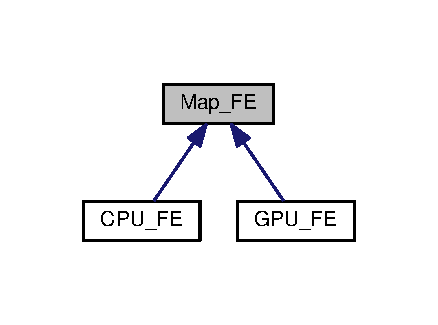
\includegraphics[width=210pt]{classMap__FE__inherit__graph}
\end{center}
\end{figure}
\subsubsection*{Public Member Functions}
\begin{DoxyCompactItemize}
\item 
virtual void \hyperlink{classMap__FE_a901af5011ef87bfd1dac3e568ef29c47}{Update} (\hyperlink{classCamera}{Camera} const \&C, rs2\+\_\+pose const \&pose, cv\+::\+Mat const \&depth)=0
\begin{DoxyCompactList}\small\item\em Method to update global map. \end{DoxyCompactList}\item 
virtual void \hyperlink{classMap__FE_aedfee41631a7287c9eb377ccb05317d6}{Points} (std\+::vector$<$ std\+::tuple$<$ float, float, float, float $>$ $>$ $\ast$points)=0
\begin{DoxyCompactList}\small\item\em Returns all points in the map. \end{DoxyCompactList}\end{DoxyCompactItemize}


\subsubsection{Detailed Description}
Virtual class Parent of \hyperlink{classCPU__FE}{C\+P\+U\+\_\+\+FE} and \hyperlink{classGPU__FE}{G\+P\+U\+\_\+\+FE} classes. 

Classes \hyperlink{classCPU__FE}{C\+P\+U\+\_\+\+FE} and \hyperlink{classGPU__FE}{G\+P\+U\+\_\+\+FE} are the front-\/end classes for C\+PU and G\+PU versions of the algorithm respectively. Both these classes inherit M\+A\+P\+\_\+\+FE, which is a virtual class\+: meaning an object of this class cannot be created. But such an implementation ensures two things\+: ~\newline

\begin{DoxyEnumerate}
\item Any implementation of any mapping algorithm must neccessarily implement the member methods of M\+A\+P\+\_\+\+FE. ~\newline

\item Other classes dependent on the global map need not change their implementation depending on the algorithm used as long as the front end of the implementation is a child of \hyperlink{classMap__FE}{Map\+\_\+\+FE}. Also pointer of a child class can be cast to their parent class. \begin{DoxySeeAlso}{See also}
\hyperlink{classCPU__FE}{C\+P\+U\+\_\+\+FE}, \hyperlink{classGPU__FE}{G\+P\+U\+\_\+\+FE} 
\end{DoxySeeAlso}

\end{DoxyEnumerate}

Definition at line \hyperlink{Helper_8hpp_source_l00082}{82} of file \hyperlink{Helper_8hpp_source}{Helper.\+hpp}.



\subsubsection{Member Function Documentation}
\index{Map\+\_\+\+FE@{Map\+\_\+\+FE}!Points@{Points}}
\index{Points@{Points}!Map\+\_\+\+FE@{Map\+\_\+\+FE}}
\paragraph[{\texorpdfstring{Points(std\+::vector$<$ std\+::tuple$<$ float, float, float, float $>$ $>$ $\ast$points)=0}{Points(std::vector< std::tuple< float, float, float, float > > *points)=0}}]{\setlength{\rightskip}{0pt plus 5cm}virtual void Map\+\_\+\+F\+E\+::\+Points (
\begin{DoxyParamCaption}
\item[{std\+::vector$<$ std\+::tuple$<$ float, float, float, float $>$ $>$ $\ast$}]{points}
\end{DoxyParamCaption}
)\hspace{0.3cm}{\ttfamily [pure virtual]}}\hypertarget{classMap__FE_aedfee41631a7287c9eb377ccb05317d6}{}\label{classMap__FE_aedfee41631a7287c9eb377ccb05317d6}


Returns all points in the map. 

Primarily to be used by \hyperlink{classLogger}{Logger} class. The points returned are in no particular order. 
\begin{DoxyParams}{Parameters}
{\em vector} & of tuple containing (x, y, z) \\
\hline
{\em variance} & of points \\
\hline
\end{DoxyParams}
\begin{DoxySeeAlso}{See also}
\hyperlink{classLogger_adcc95257ff2edceded8e272dac3603ce}{Logger\+::\+Log()} 
\end{DoxySeeAlso}


Implemented in \hyperlink{classGPU__FE_aea86626bdab826bc91b955ad6e5f6653}{G\+P\+U\+\_\+\+FE}, and \hyperlink{classCPU__FE_a4b085e590daa33cf1e2f100a58236009}{C\+P\+U\+\_\+\+FE}.



Here is the caller graph for this function\+:\nopagebreak
\begin{figure}[H]
\begin{center}
\leavevmode
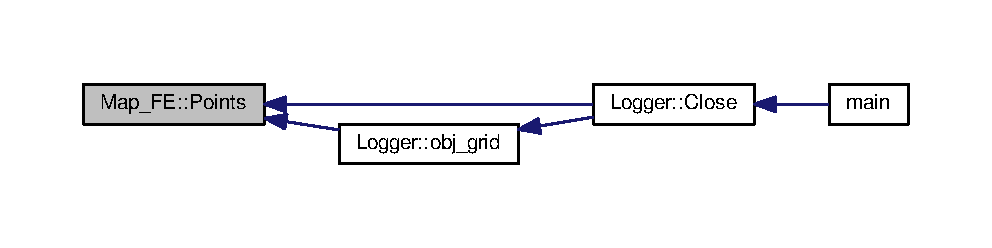
\includegraphics[width=350pt]{classMap__FE_aedfee41631a7287c9eb377ccb05317d6_icgraph}
\end{center}
\end{figure}


\index{Map\+\_\+\+FE@{Map\+\_\+\+FE}!Update@{Update}}
\index{Update@{Update}!Map\+\_\+\+FE@{Map\+\_\+\+FE}}
\paragraph[{\texorpdfstring{Update(\+Camera const \&\+C, rs2\+\_\+pose const \&pose, cv\+::\+Mat const \&depth)=0}{Update(Camera const &C, rs2_pose const &pose, cv::Mat const &depth)=0}}]{\setlength{\rightskip}{0pt plus 5cm}virtual void Map\+\_\+\+F\+E\+::\+Update (
\begin{DoxyParamCaption}
\item[{{\bf Camera} const \&}]{C, }
\item[{rs2\+\_\+pose const \&}]{pose, }
\item[{cv\+::\+Mat const \&}]{depth}
\end{DoxyParamCaption}
)\hspace{0.3cm}{\ttfamily [pure virtual]}}\hypertarget{classMap__FE_a901af5011ef87bfd1dac3e568ef29c47}{}\label{classMap__FE_a901af5011ef87bfd1dac3e568ef29c47}


Method to update global map. 

This method runs at every iteration of frame recieved at a rate of M\+A\+P\+\_\+\+U\+P\+D\+A\+T\+E\+\_\+\+R\+A\+TE. 
\begin{DoxyParams}{Parameters}
{\em \hyperlink{classCamera}{Camera}} & object \\
\hline
{\em current} & pose from T265 \\
\hline
{\em 16-\/bit} & (default) depth image from D435 \\
\hline
\end{DoxyParams}


Implemented in \hyperlink{classGPU__FE_aa9039bd613961d4e0911b8514ed14fba}{G\+P\+U\+\_\+\+FE}, and \hyperlink{classCPU__FE_aae7cb60a405b294a680a929ecff5c2ae}{C\+P\+U\+\_\+\+FE}.



Here is the caller graph for this function\+:\nopagebreak
\begin{figure}[H]
\begin{center}
\leavevmode
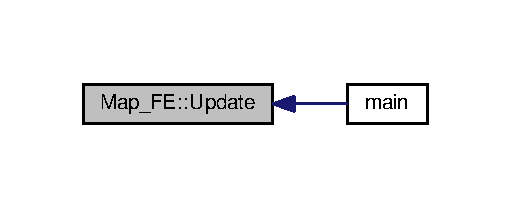
\includegraphics[width=245pt]{classMap__FE_a901af5011ef87bfd1dac3e568ef29c47_icgraph}
\end{center}
\end{figure}




The documentation for this class was generated from the following file\+:\begin{DoxyCompactItemize}
\item 
include/\hyperlink{Helper_8hpp}{Helper.\+hpp}\end{DoxyCompactItemize}

\hypertarget{classocc__grid}{}\subsection{occ\+\_\+grid Class Reference}
\label{classocc__grid}\index{occ\+\_\+grid@{occ\+\_\+grid}}


The top-\/most class managing the global map.  




{\ttfamily \#include $<$Voxel.\+hpp$>$}



Collaboration diagram for occ\+\_\+grid\+:\nopagebreak
\begin{figure}[H]
\begin{center}
\leavevmode
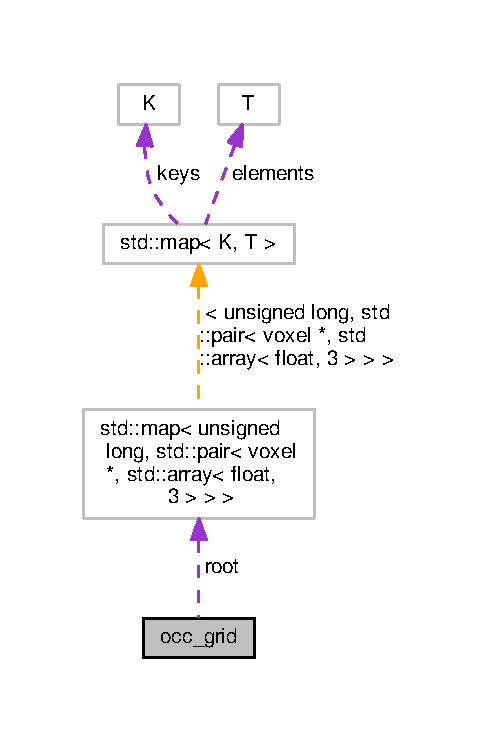
\includegraphics[width=230pt]{classocc__grid__coll__graph}
\end{center}
\end{figure}
\subsubsection*{Public Member Functions}
\begin{DoxyCompactItemize}
\item 
\hyperlink{classocc__grid_a2bd8f966cb86730569eef2322e4fe263}{occ\+\_\+grid} ()
\begin{DoxyCompactList}\small\item\em Default Constructor. \end{DoxyCompactList}\item 
void \hyperlink{classocc__grid_aaf38d339d7d1b3226d9673f8d6102b2c}{update\+\_\+point} (float x, float y, float z)
\begin{DoxyCompactList}\small\item\em Updates point in the global map. \end{DoxyCompactList}\item 
void \hyperlink{classocc__grid_a8b47af213fb57bf31c21ab1a9ef36505}{all\+\_\+points} (std\+::vector$<$ std\+::tuple$<$ float, float, float, float $>$ $>$ $\ast$set)
\begin{DoxyCompactList}\small\item\em Appends points to the vector of points. \end{DoxyCompactList}\item 
void \hyperlink{classocc__grid_adbfab59a1fb247d53a993fd9a2a26d67}{free\+\_\+mem} ()
\begin{DoxyCompactList}\small\item\em Deletes the global map. \end{DoxyCompactList}\item 
unsigned long \hyperlink{classocc__grid_a0fb045d82217675decfc9b9289ad35ea}{index} (std\+::array$<$ float, 3 $>$ p)
\begin{DoxyCompactList}\small\item\em Calculates index used as key to index into root. \end{DoxyCompactList}\item 
std\+::array$<$ float, 3 $>$ \hyperlink{classocc__grid_abf7ece8bcafa68e1292b0be52a5d9996}{mod\+\_\+p} (std\+::array$<$ float, 3 $>$ p)
\begin{DoxyCompactList}\small\item\em Calculates co-\/ordinate of point modulo edge length. \end{DoxyCompactList}\end{DoxyCompactItemize}
\subsubsection*{Public Attributes}
\begin{DoxyCompactItemize}
\item 
std\+::map$<$ unsigned long, std\+::pair$<$ \hyperlink{classvoxel}{voxel} $\ast$, std\+::array$<$ float, 3 $>$ $>$ $>$ \hyperlink{classocc__grid_ae5ebfc317affec175dba9d27f5fcf2fa}{root}
\begin{DoxyCompactList}\small\item\em Array of pointers and origins of root voxels. \end{DoxyCompactList}\end{DoxyCompactItemize}


\subsubsection{Detailed Description}
The top-\/most class managing the global map. 

An object of this class maintains the map. This class is specific to the C\+PU mode of operation and can be thought of as an interface between the user and the global map. A map, which is a red-\/black tree, is maintained, containing all the root voxels in the map. The equivalent of this class for G\+PU code are the {\bfseries global} methods called from the host on the device. 

Definition at line \hyperlink{Voxel_8hpp_source_l00351}{351} of file \hyperlink{Voxel_8hpp_source}{Voxel.\+hpp}.



\subsubsection{Constructor \& Destructor Documentation}
\index{occ\+\_\+grid@{occ\+\_\+grid}!occ\+\_\+grid@{occ\+\_\+grid}}
\index{occ\+\_\+grid@{occ\+\_\+grid}!occ\+\_\+grid@{occ\+\_\+grid}}
\paragraph[{\texorpdfstring{occ\+\_\+grid()}{occ_grid()}}]{\setlength{\rightskip}{0pt plus 5cm}occ\+\_\+grid\+::occ\+\_\+grid (
\begin{DoxyParamCaption}
{}
\end{DoxyParamCaption}
)\hspace{0.3cm}{\ttfamily [inline]}}\hypertarget{classocc__grid_a2bd8f966cb86730569eef2322e4fe263}{}\label{classocc__grid_a2bd8f966cb86730569eef2322e4fe263}


Default Constructor. 



Definition at line \hyperlink{Voxel_8hpp_source_l00365}{365} of file \hyperlink{Voxel_8hpp_source}{Voxel.\+hpp}.



\subsubsection{Member Function Documentation}
\index{occ\+\_\+grid@{occ\+\_\+grid}!all\+\_\+points@{all\+\_\+points}}
\index{all\+\_\+points@{all\+\_\+points}!occ\+\_\+grid@{occ\+\_\+grid}}
\paragraph[{\texorpdfstring{all\+\_\+points(std\+::vector$<$ std\+::tuple$<$ float, float, float, float $>$ $>$ $\ast$set)}{all_points(std::vector< std::tuple< float, float, float, float > > *set)}}]{\setlength{\rightskip}{0pt plus 5cm}void occ\+\_\+grid\+::all\+\_\+points (
\begin{DoxyParamCaption}
\item[{std\+::vector$<$ std\+::tuple$<$ float, float, float, float $>$ $>$ $\ast$}]{set}
\end{DoxyParamCaption}
)\hspace{0.3cm}{\ttfamily [inline]}}\hypertarget{classocc__grid_a8b47af213fb57bf31c21ab1a9ef36505}{}\label{classocc__grid_a8b47af213fb57bf31c21ab1a9ef36505}


Appends points to the vector of points. 

This method recursively calls \hyperlink{classvoxel_a4189fb0f24ad9eba1447e2ebf8ee0015}{voxel\+::all\+\_\+points()}, to append all the points in the leaf nodes to the vector. This method is called from \hyperlink{classCPU__FE_a4b085e590daa33cf1e2f100a58236009}{C\+P\+U\+\_\+\+F\+E\+::\+Points()} 
\begin{DoxyParams}{Parameters}
{\em vector} & of point co-\/ordinates \\
\hline
\end{DoxyParams}
\begin{DoxySeeAlso}{See also}
\hyperlink{classvoxel_a4189fb0f24ad9eba1447e2ebf8ee0015}{voxel\+::all\+\_\+points()}, \hyperlink{classCPU__FE_a4b085e590daa33cf1e2f100a58236009}{C\+P\+U\+\_\+\+F\+E\+::\+Points()} 
\end{DoxySeeAlso}


Definition at line \hyperlink{Voxel_8hpp_source_l00397}{397} of file \hyperlink{Voxel_8hpp_source}{Voxel.\+hpp}.



Here is the caller graph for this function\+:\nopagebreak
\begin{figure}[H]
\begin{center}
\leavevmode
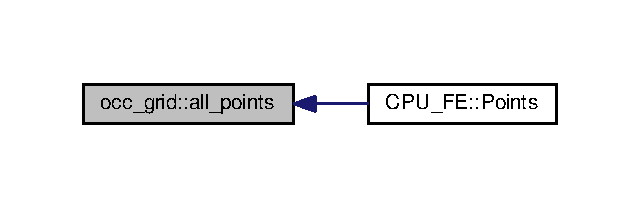
\includegraphics[width=307pt]{classocc__grid_a8b47af213fb57bf31c21ab1a9ef36505_icgraph}
\end{center}
\end{figure}


\index{occ\+\_\+grid@{occ\+\_\+grid}!free\+\_\+mem@{free\+\_\+mem}}
\index{free\+\_\+mem@{free\+\_\+mem}!occ\+\_\+grid@{occ\+\_\+grid}}
\paragraph[{\texorpdfstring{free\+\_\+mem()}{free_mem()}}]{\setlength{\rightskip}{0pt plus 5cm}void occ\+\_\+grid\+::free\+\_\+mem (
\begin{DoxyParamCaption}
{}
\end{DoxyParamCaption}
)\hspace{0.3cm}{\ttfamily [inline]}}\hypertarget{classocc__grid_adbfab59a1fb247d53a993fd9a2a26d67}{}\label{classocc__grid_adbfab59a1fb247d53a993fd9a2a26d67}


Deletes the global map. 

This method recursively calls \hyperlink{classvoxel_aff25abf72186eb31821d1ffacf557c67}{voxel\+::free\+\_\+mem()}, to delete all the nodes in the octree. This method is called from \hyperlink{classCPU__FE_a425dc3014e22d7aeaaf261ac945f4da1}{C\+P\+U\+\_\+\+F\+E\+::$\sim$\+C\+P\+U\+\_\+\+F\+E()} \begin{DoxySeeAlso}{See also}
\hyperlink{classvoxel_aff25abf72186eb31821d1ffacf557c67}{voxel\+::free\+\_\+mem()}, \hyperlink{classCPU__FE_a425dc3014e22d7aeaaf261ac945f4da1}{C\+P\+U\+\_\+\+F\+E\+::$\sim$\+C\+P\+U\+\_\+\+F\+E()} 
\end{DoxySeeAlso}


Definition at line \hyperlink{Voxel_8hpp_source_l00409}{409} of file \hyperlink{Voxel_8hpp_source}{Voxel.\+hpp}.



Here is the caller graph for this function\+:\nopagebreak
\begin{figure}[H]
\begin{center}
\leavevmode
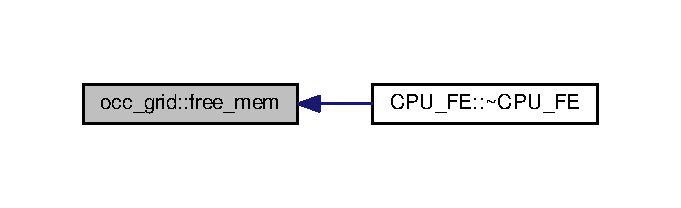
\includegraphics[width=327pt]{classocc__grid_adbfab59a1fb247d53a993fd9a2a26d67_icgraph}
\end{center}
\end{figure}


\index{occ\+\_\+grid@{occ\+\_\+grid}!index@{index}}
\index{index@{index}!occ\+\_\+grid@{occ\+\_\+grid}}
\paragraph[{\texorpdfstring{index(std\+::array$<$ float, 3 $>$ p)}{index(std::array< float, 3 > p)}}]{\setlength{\rightskip}{0pt plus 5cm}unsigned long occ\+\_\+grid\+::index (
\begin{DoxyParamCaption}
\item[{std\+::array$<$ float, 3 $>$}]{p}
\end{DoxyParamCaption}
)\hspace{0.3cm}{\ttfamily [inline]}}\hypertarget{classocc__grid_a0fb045d82217675decfc9b9289ad35ea}{}\label{classocc__grid_a0fb045d82217675decfc9b9289ad35ea}


Calculates index used as key to index into root. 

This is used to calculate a unique whole number from a set of three integers\+: indices of origin of the voxel. Instead of using three nested maps each trying to index one co-\/ordinate at each level ( $ O(\ln(N_x)+\ln(N_y)+\ln(N_z))$), a bijective mapping from $ \mathbb{Z}^{3} \to \mathbb{N}$ is defined. Although the order of the complexity remains the same, the look-\/up is guaranteed to occur in less time than the previous case. 
\begin{DoxyParams}{Parameters}
{\em co-\/ordinates} & of the origin of voxel \\
\hline
\end{DoxyParams}
\begin{DoxyReturn}{Returns}
index of point 
\end{DoxyReturn}
\begin{DoxySeeAlso}{See also}
\hyperlink{classocc__grid_aaf38d339d7d1b3226d9673f8d6102b2c}{occ\+\_\+grid\+::update\+\_\+point()}, \hyperlink{classocc__grid_ae5ebfc317affec175dba9d27f5fcf2fa}{root} 
\end{DoxySeeAlso}


Definition at line \hyperlink{Voxel_8hpp_source_l00435}{435} of file \hyperlink{Voxel_8hpp_source}{Voxel.\+hpp}.



Here is the call graph for this function\+:\nopagebreak
\begin{figure}[H]
\begin{center}
\leavevmode
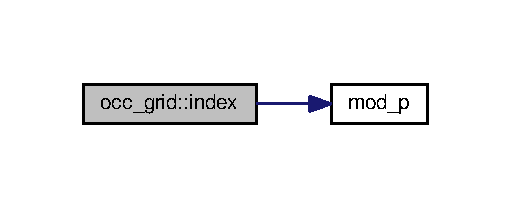
\includegraphics[width=245pt]{classocc__grid_a0fb045d82217675decfc9b9289ad35ea_cgraph}
\end{center}
\end{figure}


\index{occ\+\_\+grid@{occ\+\_\+grid}!mod\+\_\+p@{mod\+\_\+p}}
\index{mod\+\_\+p@{mod\+\_\+p}!occ\+\_\+grid@{occ\+\_\+grid}}
\paragraph[{\texorpdfstring{mod\+\_\+p(std\+::array$<$ float, 3 $>$ p)}{mod_p(std::array< float, 3 > p)}}]{\setlength{\rightskip}{0pt plus 5cm}std\+::array$<$float, 3$>$ occ\+\_\+grid\+::mod\+\_\+p (
\begin{DoxyParamCaption}
\item[{std\+::array$<$ float, 3 $>$}]{p}
\end{DoxyParamCaption}
)\hspace{0.3cm}{\ttfamily [inline]}}\hypertarget{classocc__grid_abf7ece8bcafa68e1292b0be52a5d9996}{}\label{classocc__grid_abf7ece8bcafa68e1292b0be52a5d9996}


Calculates co-\/ordinate of point modulo edge length. 

Returns $p \mod VOX\_L[0, 1)^3$ 
\begin{DoxyParams}{Parameters}
{\em co-\/ordinate} & of point \\
\hline
\end{DoxyParams}
\begin{DoxyReturn}{Returns}
modulo of co-\/ordinate of point 
\end{DoxyReturn}


Definition at line \hyperlink{Voxel_8hpp_source_l00449}{449} of file \hyperlink{Voxel_8hpp_source}{Voxel.\+hpp}.

\index{occ\+\_\+grid@{occ\+\_\+grid}!update\+\_\+point@{update\+\_\+point}}
\index{update\+\_\+point@{update\+\_\+point}!occ\+\_\+grid@{occ\+\_\+grid}}
\paragraph[{\texorpdfstring{update\+\_\+point(float x, float y, float z)}{update_point(float x, float y, float z)}}]{\setlength{\rightskip}{0pt plus 5cm}void occ\+\_\+grid\+::update\+\_\+point (
\begin{DoxyParamCaption}
\item[{float}]{x, }
\item[{float}]{y, }
\item[{float}]{z}
\end{DoxyParamCaption}
)\hspace{0.3cm}{\ttfamily [inline]}}\hypertarget{classocc__grid_aaf38d339d7d1b3226d9673f8d6102b2c}{}\label{classocc__grid_aaf38d339d7d1b3226d9673f8d6102b2c}


Updates point in the global map. 

This method recursively calls \hyperlink{classvoxel_a97737aec7c381e72d929d2f084952683}{voxel\+::update\+\_\+vox()}, to update the point in the respective voxel. This method itself is called upon by \hyperlink{classCPU__FE_aae7cb60a405b294a680a929ecff5c2ae}{C\+P\+U\+\_\+\+F\+E\+::\+Update()}. The information on the origin of the voxel is used to identify the voxel, and the index is used as a key to search in the red-\/black tree. This method is the same as \hyperlink{classvoxel_a97737aec7c381e72d929d2f084952683}{voxel\+::update\+\_\+vox()}, other than the fact that the point doesn\textquotesingle{}t directly map to any \char`\"{}child\char`\"{} voxel. 
\begin{DoxyParams}{Parameters}
{\em global} & co-\/ordinates of the point to be updated \\
\hline
\end{DoxyParams}
\begin{DoxySeeAlso}{See also}
\hyperlink{classocc__grid_a0fb045d82217675decfc9b9289ad35ea}{index()}, \hyperlink{classvoxel_a97737aec7c381e72d929d2f084952683}{voxel\+::update\+\_\+vox()}, \hyperlink{classCPU__FE_aae7cb60a405b294a680a929ecff5c2ae}{C\+P\+U\+\_\+\+F\+E\+::\+Update()} 
\end{DoxySeeAlso}


Definition at line \hyperlink{Voxel_8hpp_source_l00376}{376} of file \hyperlink{Voxel_8hpp_source}{Voxel.\+hpp}.



Here is the call graph for this function\+:\nopagebreak
\begin{figure}[H]
\begin{center}
\leavevmode
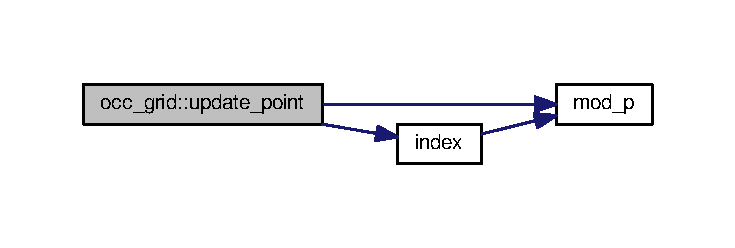
\includegraphics[width=350pt]{classocc__grid_aaf38d339d7d1b3226d9673f8d6102b2c_cgraph}
\end{center}
\end{figure}




Here is the caller graph for this function\+:\nopagebreak
\begin{figure}[H]
\begin{center}
\leavevmode
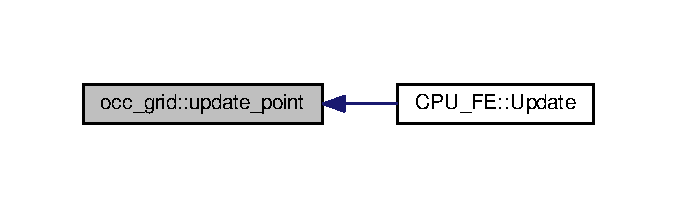
\includegraphics[width=325pt]{classocc__grid_aaf38d339d7d1b3226d9673f8d6102b2c_icgraph}
\end{center}
\end{figure}




\subsubsection{Member Data Documentation}
\index{occ\+\_\+grid@{occ\+\_\+grid}!root@{root}}
\index{root@{root}!occ\+\_\+grid@{occ\+\_\+grid}}
\paragraph[{\texorpdfstring{root}{root}}]{\setlength{\rightskip}{0pt plus 5cm}std\+::map$<$ unsigned long, std\+::pair$<${\bf voxel} $\ast$, std\+::array$<$float, 3$>$ $>$ $>$ occ\+\_\+grid\+::root}\hypertarget{classocc__grid_ae5ebfc317affec175dba9d27f5fcf2fa}{}\label{classocc__grid_ae5ebfc317affec175dba9d27f5fcf2fa}


Array of pointers and origins of root voxels. 

This map contains an index calculated from the origin of the root voxel as the key, and a pair containing pointer to root voxel and the co-\/ordinates of the origin of the voxel. A key-\/value paradigm is used in order to implement a red-\/black tree, which brings down look-\/up time from $O(n)$ to $O(\ln(n))$. The index is a unique whole number calculated using the origin of the voxel. \begin{DoxySeeAlso}{See also}
\hyperlink{classocc__grid_a0fb045d82217675decfc9b9289ad35ea}{occ\+\_\+grid\+::index()} 
\end{DoxySeeAlso}


Definition at line \hyperlink{Voxel_8hpp_source_l00362}{362} of file \hyperlink{Voxel_8hpp_source}{Voxel.\+hpp}.



The documentation for this class was generated from the following file\+:\begin{DoxyCompactItemize}
\item 
include/\hyperlink{Voxel_8hpp}{Voxel.\+hpp}\end{DoxyCompactItemize}

\hypertarget{classPair}{}\subsection{Pair$<$ A, B $>$ Class Template Reference}
\label{classPair}\index{Pair$<$ A, B $>$@{Pair$<$ A, B $>$}}


Template Class for Pairs.  




{\ttfamily \#include $<$Helper.\+hpp$>$}



Inheritance diagram for Pair$<$ A, B $>$\+:\nopagebreak
\begin{figure}[H]
\begin{center}
\leavevmode
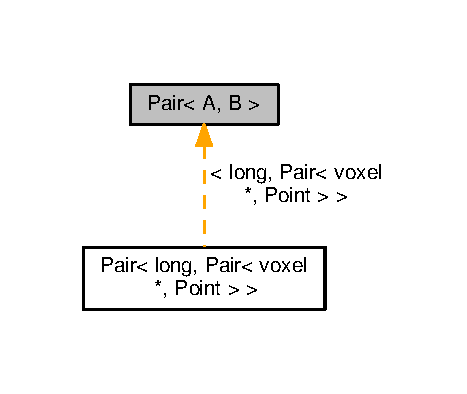
\includegraphics[width=224pt]{classPair__inherit__graph}
\end{center}
\end{figure}
\subsubsection*{Public Member Functions}
\begin{Indent}{\bf Constructors}\par
\begin{DoxyCompactItemize}
\item 
\hyperlink{Helper_8hpp_a0029886fd5e151820efb6eb46c000466}{C\+U\+D\+A\+\_\+\+C\+A\+LL} \hyperlink{classPair_ab76fff1f93ef8974bec7430bd67b916d}{Pair} ()=default
\begin{DoxyCompactList}\small\item\em Default Constructor. \end{DoxyCompactList}\item 
\hyperlink{Helper_8hpp_a0029886fd5e151820efb6eb46c000466}{C\+U\+D\+A\+\_\+\+C\+A\+LL} \hyperlink{classPair_addd8fa451e9cc9e1ab0ee13ccb130966}{Pair} (const A a, const B b)
\begin{DoxyCompactList}\small\item\em Equivalent to \hyperlink{classPair_ab76fff1f93ef8974bec7430bd67b916d}{Pair()}, Pair.\+A(a), Pair.\+B(b) \end{DoxyCompactList}\end{DoxyCompactItemize}
\end{Indent}
\begin{Indent}{\bf Operator Overrides}\par
\begin{DoxyCompactItemize}
\item 
\hyperlink{Helper_8hpp_a0029886fd5e151820efb6eb46c000466}{C\+U\+D\+A\+\_\+\+C\+A\+LL} bool \hyperlink{classPair_ab2e5000f2ce579285f773fafca762fb7}{operator$<$} (\hyperlink{classPair}{Pair}$<$ A, B $>$ const \&P) const 
\begin{DoxyCompactList}\small\item\em overridding of \textquotesingle{}$<$\textquotesingle{} operator. \end{DoxyCompactList}\item 
\hyperlink{Helper_8hpp_a0029886fd5e151820efb6eb46c000466}{C\+U\+D\+A\+\_\+\+C\+A\+LL} bool \hyperlink{classPair_a8e382aa87f8063084ecea74136a35ace}{operator==} (\hyperlink{classPair}{Pair}$<$ A, B $>$ const \&P) const 
\begin{DoxyCompactList}\small\item\em overridding of \textquotesingle{}==\textquotesingle{} operator. \end{DoxyCompactList}\end{DoxyCompactItemize}
\end{Indent}
\subsubsection*{Public Attributes}
\begin{DoxyCompactItemize}
\item 
A \hyperlink{classPair_a98924311a2986df358d3b1965f8abd06}{first}
\begin{DoxyCompactList}\small\item\em First member of \hyperlink{classPair}{Pair}. Can be used as an index. \end{DoxyCompactList}\item 
B \hyperlink{classPair_af49ec2d61a46cad5cd1227dba4932aff}{second}
\begin{DoxyCompactList}\small\item\em Second member of \hyperlink{classPair}{Pair}. Can be used as mapped value. \end{DoxyCompactList}\end{DoxyCompactItemize}


\subsubsection{Detailed Description}
\subsubsection*{template$<$typename A, typename B$>$\\*
class Pair$<$ A, B $>$}

Template Class for Pairs. 

This class is used as a replacement for std\+::pair for C\+U\+DA code. Note that S\+TL classes and methods should preferably not used in C\+U\+DA as they might cause memory access errors. The \textquotesingle{}$<$\textquotesingle{} operator is defined on Pair.\+first, so \textquotesingle{}$<$\textquotesingle{} should be defined for template class A. This is used to sort a vector of this template class in C\+U\+DA as a replacement for std\+::map -\/ which uses a red-\/black tree implementation. \begin{DoxySeeAlso}{See also}
\hyperlink{classGPU__FE_aa9039bd613961d4e0911b8514ed14fba}{G\+P\+U\+\_\+\+F\+E\+::\+Update()} 
\end{DoxySeeAlso}


Definition at line \hyperlink{Helper_8hpp_source_l00026}{26} of file \hyperlink{Helper_8hpp_source}{Helper.\+hpp}.



\subsubsection{Constructor \& Destructor Documentation}
\index{Pair@{Pair}!Pair@{Pair}}
\index{Pair@{Pair}!Pair@{Pair}}
\paragraph[{\texorpdfstring{Pair()=default}{Pair()=default}}]{\setlength{\rightskip}{0pt plus 5cm}template$<$typename A, typename B$>$ {\bf C\+U\+D\+A\+\_\+\+C\+A\+LL} {\bf Pair}$<$ A, B $>$\+::{\bf Pair} (
\begin{DoxyParamCaption}
{}
\end{DoxyParamCaption}
)\hspace{0.3cm}{\ttfamily [default]}}\hypertarget{classPair_ab76fff1f93ef8974bec7430bd67b916d}{}\label{classPair_ab76fff1f93ef8974bec7430bd67b916d}


Default Constructor. 

\index{Pair@{Pair}!Pair@{Pair}}
\index{Pair@{Pair}!Pair@{Pair}}
\paragraph[{\texorpdfstring{Pair(const A a, const B b)}{Pair(const A a, const B b)}}]{\setlength{\rightskip}{0pt plus 5cm}template$<$typename A, typename B$>$ {\bf C\+U\+D\+A\+\_\+\+C\+A\+LL} {\bf Pair}$<$ A, B $>$\+::{\bf Pair} (
\begin{DoxyParamCaption}
\item[{const A}]{a, }
\item[{const B}]{b}
\end{DoxyParamCaption}
)\hspace{0.3cm}{\ttfamily [inline]}}\hypertarget{classPair_addd8fa451e9cc9e1ab0ee13ccb130966}{}\label{classPair_addd8fa451e9cc9e1ab0ee13ccb130966}


Equivalent to \hyperlink{classPair_ab76fff1f93ef8974bec7430bd67b916d}{Pair()}, Pair.\+A(a), Pair.\+B(b) 


\begin{DoxyParams}{Parameters}
{\em object} & of type A \\
\hline
{\em object} & of type B \\
\hline
\end{DoxyParams}


Definition at line \hyperlink{Helper_8hpp_source_l00046}{46} of file \hyperlink{Helper_8hpp_source}{Helper.\+hpp}.



\subsubsection{Member Function Documentation}
\index{Pair@{Pair}!operator$<$@{operator$<$}}
\index{operator$<$@{operator$<$}!Pair@{Pair}}
\paragraph[{\texorpdfstring{operator$<$(\+Pair$<$ A, B $>$ const \&\+P) const }{operator<(Pair< A, B > const &P) const }}]{\setlength{\rightskip}{0pt plus 5cm}template$<$typename A, typename B$>$ {\bf C\+U\+D\+A\+\_\+\+C\+A\+LL} bool {\bf Pair}$<$ A, B $>$\+::operator$<$ (
\begin{DoxyParamCaption}
\item[{{\bf Pair}$<$ A, B $>$ const \&}]{P}
\end{DoxyParamCaption}
) const\hspace{0.3cm}{\ttfamily [inline]}}\hypertarget{classPair_ab2e5000f2ce579285f773fafca762fb7}{}\label{classPair_ab2e5000f2ce579285f773fafca762fb7}


overridding of \textquotesingle{}$<$\textquotesingle{} operator. 

Used to sort vectors of element type Pair$<$\+A,\+B$>$. 
\begin{DoxyParams}{Parameters}
{\em \hyperlink{classPair}{Pair}} & P of types A, and B \\
\hline
\end{DoxyParams}
\begin{DoxyReturn}{Returns}
boolean value comparing the first elements 
\end{DoxyReturn}
\begin{DoxySeeAlso}{See also}
\hyperlink{classGPU__FE_aa9039bd613961d4e0911b8514ed14fba}{G\+P\+U\+\_\+\+F\+E\+::\+Update()} 
\end{DoxySeeAlso}


Definition at line \hyperlink{Helper_8hpp_source_l00059}{59} of file \hyperlink{Helper_8hpp_source}{Helper.\+hpp}.

\index{Pair@{Pair}!operator==@{operator==}}
\index{operator==@{operator==}!Pair@{Pair}}
\paragraph[{\texorpdfstring{operator==(\+Pair$<$ A, B $>$ const \&\+P) const }{operator==(Pair< A, B > const &P) const }}]{\setlength{\rightskip}{0pt plus 5cm}template$<$typename A, typename B$>$ {\bf C\+U\+D\+A\+\_\+\+C\+A\+LL} bool {\bf Pair}$<$ A, B $>$\+::operator== (
\begin{DoxyParamCaption}
\item[{{\bf Pair}$<$ A, B $>$ const \&}]{P}
\end{DoxyParamCaption}
) const\hspace{0.3cm}{\ttfamily [inline]}}\hypertarget{classPair_a8e382aa87f8063084ecea74136a35ace}{}\label{classPair_a8e382aa87f8063084ecea74136a35ace}


overridding of \textquotesingle{}==\textquotesingle{} operator. 



Definition at line \hyperlink{Helper_8hpp_source_l00064}{64} of file \hyperlink{Helper_8hpp_source}{Helper.\+hpp}.



\subsubsection{Member Data Documentation}
\index{Pair@{Pair}!first@{first}}
\index{first@{first}!Pair@{Pair}}
\paragraph[{\texorpdfstring{first}{first}}]{\setlength{\rightskip}{0pt plus 5cm}template$<$typename A, typename B$>$ A {\bf Pair}$<$ A, B $>$\+::first}\hypertarget{classPair_a98924311a2986df358d3b1965f8abd06}{}\label{classPair_a98924311a2986df358d3b1965f8abd06}


First member of \hyperlink{classPair}{Pair}. Can be used as an index. 



Definition at line \hyperlink{Helper_8hpp_source_l00031}{31} of file \hyperlink{Helper_8hpp_source}{Helper.\+hpp}.

\index{Pair@{Pair}!second@{second}}
\index{second@{second}!Pair@{Pair}}
\paragraph[{\texorpdfstring{second}{second}}]{\setlength{\rightskip}{0pt plus 5cm}template$<$typename A, typename B$>$ B {\bf Pair}$<$ A, B $>$\+::second}\hypertarget{classPair_af49ec2d61a46cad5cd1227dba4932aff}{}\label{classPair_af49ec2d61a46cad5cd1227dba4932aff}


Second member of \hyperlink{classPair}{Pair}. Can be used as mapped value. 



Definition at line \hyperlink{Helper_8hpp_source_l00033}{33} of file \hyperlink{Helper_8hpp_source}{Helper.\+hpp}.



The documentation for this class was generated from the following file\+:\begin{DoxyCompactItemize}
\item 
include/\hyperlink{Helper_8hpp}{Helper.\+hpp}\end{DoxyCompactItemize}

\hypertarget{structPoint}{}\subsection{Point Struct Reference}
\label{structPoint}\index{Point@{Point}}


\hyperlink{structPoint}{Point} co-\/ordinates.  


\subsubsection*{Public Attributes}
\begin{Indent}{\bf Point co-\/ordinates}\par
\begin{DoxyCompactItemize}
\item 
float \hyperlink{structPoint_a05dfe2dfbde813ad234b514f30e662f1}{x}
\item 
float \hyperlink{structPoint_a6101960c8d2d4e8ea1d32c9234bbeb8d}{y}
\item 
float \hyperlink{structPoint_a9a666531e0e99adff132be93d2407d0c}{z}
\end{DoxyCompactItemize}
\end{Indent}


\subsubsection{Detailed Description}
\hyperlink{structPoint}{Point} co-\/ordinates. 

Used to pass to C\+U\+DA kernel 

Definition at line \hyperlink{Voxel_8cuh_source_l00172}{172} of file \hyperlink{Voxel_8cuh_source}{Voxel.\+cuh}.



\subsubsection{Member Data Documentation}
\index{Point@{Point}!x@{x}}
\index{x@{x}!Point@{Point}}
\paragraph[{\texorpdfstring{x}{x}}]{\setlength{\rightskip}{0pt plus 5cm}float Point\+::x}\hypertarget{structPoint_a05dfe2dfbde813ad234b514f30e662f1}{}\label{structPoint_a05dfe2dfbde813ad234b514f30e662f1}


Definition at line \hyperlink{Voxel_8cuh_source_l00177}{177} of file \hyperlink{Voxel_8cuh_source}{Voxel.\+cuh}.

\index{Point@{Point}!y@{y}}
\index{y@{y}!Point@{Point}}
\paragraph[{\texorpdfstring{y}{y}}]{\setlength{\rightskip}{0pt plus 5cm}float Point\+::y}\hypertarget{structPoint_a6101960c8d2d4e8ea1d32c9234bbeb8d}{}\label{structPoint_a6101960c8d2d4e8ea1d32c9234bbeb8d}


Definition at line \hyperlink{Voxel_8cuh_source_l00177}{177} of file \hyperlink{Voxel_8cuh_source}{Voxel.\+cuh}.

\index{Point@{Point}!z@{z}}
\index{z@{z}!Point@{Point}}
\paragraph[{\texorpdfstring{z}{z}}]{\setlength{\rightskip}{0pt plus 5cm}float Point\+::z}\hypertarget{structPoint_a9a666531e0e99adff132be93d2407d0c}{}\label{structPoint_a9a666531e0e99adff132be93d2407d0c}


Definition at line \hyperlink{Voxel_8cuh_source_l00177}{177} of file \hyperlink{Voxel_8cuh_source}{Voxel.\+cuh}.



The documentation for this struct was generated from the following file\+:\begin{DoxyCompactItemize}
\item 
include/\hyperlink{Voxel_8cuh}{Voxel.\+cuh}\end{DoxyCompactItemize}

\hypertarget{structPose}{}\subsection{Pose Struct Reference}
\label{structPose}\index{Pose@{Pose}}


\hyperlink{structPose}{Pose} of T265 camera.  




Collaboration diagram for Pose\+:\nopagebreak
\begin{figure}[H]
\begin{center}
\leavevmode
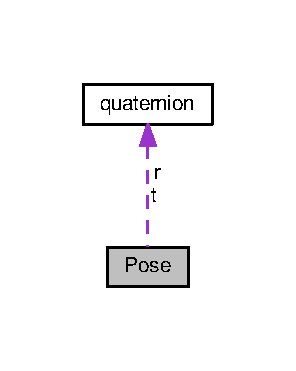
\includegraphics[width=142pt]{structPose__coll__graph}
\end{center}
\end{figure}
\subsubsection*{Public Attributes}
\begin{DoxyCompactItemize}
\item 
\hyperlink{classquaternion}{quaternion} \hyperlink{structPose_aa87ab4baa5bab93b316c8ef417b6f1ef}{t}
\begin{DoxyCompactList}\small\item\em Translation of T265 expressed as a quaternion in T265 frame. \end{DoxyCompactList}\item 
\hyperlink{classquaternion}{quaternion} \hyperlink{structPose_ac86b5844a0203b03971005be99e59388}{r}
\begin{DoxyCompactList}\small\item\em Rotation of T265 expressed as a quaternion in T265 frame. \end{DoxyCompactList}\end{DoxyCompactItemize}


\subsubsection{Detailed Description}
\hyperlink{structPose}{Pose} of T265 camera. 

Used to pass to C\+U\+DA kernel 

Definition at line \hyperlink{Voxel_8cuh_source_l00120}{120} of file \hyperlink{Voxel_8cuh_source}{Voxel.\+cuh}.



\subsubsection{Member Data Documentation}
\index{Pose@{Pose}!r@{r}}
\index{r@{r}!Pose@{Pose}}
\paragraph[{\texorpdfstring{r}{r}}]{\setlength{\rightskip}{0pt plus 5cm}{\bf quaternion} Pose\+::r}\hypertarget{structPose_ac86b5844a0203b03971005be99e59388}{}\label{structPose_ac86b5844a0203b03971005be99e59388}


Rotation of T265 expressed as a quaternion in T265 frame. 



Definition at line \hyperlink{Voxel_8cuh_source_l00124}{124} of file \hyperlink{Voxel_8cuh_source}{Voxel.\+cuh}.

\index{Pose@{Pose}!t@{t}}
\index{t@{t}!Pose@{Pose}}
\paragraph[{\texorpdfstring{t}{t}}]{\setlength{\rightskip}{0pt plus 5cm}{\bf quaternion} Pose\+::t}\hypertarget{structPose_aa87ab4baa5bab93b316c8ef417b6f1ef}{}\label{structPose_aa87ab4baa5bab93b316c8ef417b6f1ef}


Translation of T265 expressed as a quaternion in T265 frame. 



Definition at line \hyperlink{Voxel_8cuh_source_l00122}{122} of file \hyperlink{Voxel_8cuh_source}{Voxel.\+cuh}.



The documentation for this struct was generated from the following file\+:\begin{DoxyCompactItemize}
\item 
include/\hyperlink{Voxel_8cuh}{Voxel.\+cuh}\end{DoxyCompactItemize}

\hypertarget{classquaternion}{}\subsection{quaternion Class Reference}
\label{classquaternion}\index{quaternion@{quaternion}}


A basic Quaternion class.  




{\ttfamily \#include $<$Voxel.\+hpp$>$}

\subsubsection*{Public Member Functions}
\begin{DoxyCompactItemize}
\item 
\+\_\+\+\_\+host\+\_\+\+\_\+ \+\_\+\+\_\+device\+\_\+\+\_\+ \hyperlink{classquaternion_a01adb7930c2003b777cb91a7182c482e}{quaternion} (float \hyperlink{classquaternion_acdcda48f9dd7ff35873aae38fa33ab78}{x}, float \hyperlink{classquaternion_a48e3d1fbf5e12eb54985c32b45dd8303}{y}, float \hyperlink{classquaternion_a538598007238d399f79ddcecd39ef5cf}{z}, float \hyperlink{classquaternion_ab2b38aca1971114e0ba4218b75d7f472}{w})
\begin{DoxyCompactList}\small\item\em Constructor taking x, y, z, w in order. \end{DoxyCompactList}\item 
\+\_\+\+\_\+host\+\_\+\+\_\+ \+\_\+\+\_\+device\+\_\+\+\_\+ \hyperlink{classquaternion}{quaternion} \hyperlink{classquaternion_a5f2dff4e0f446d05e826a63d5a45d230}{inv} ()
\begin{DoxyCompactList}\small\item\em Inverse of the quaternion. \end{DoxyCompactList}\item 
\+\_\+\+\_\+host\+\_\+\+\_\+ \+\_\+\+\_\+device\+\_\+\+\_\+ \hyperlink{classquaternion}{quaternion} \hyperlink{classquaternion_a63777bf9c0c0a269852808442c2be4f5}{operator$\ast$} (\hyperlink{classquaternion}{quaternion} const \&q)
\begin{DoxyCompactList}\small\item\em $\times$ operator \end{DoxyCompactList}\item 
\+\_\+\+\_\+host\+\_\+\+\_\+ \+\_\+\+\_\+device\+\_\+\+\_\+ \hyperlink{classquaternion}{quaternion} \hyperlink{classquaternion_ae2cf533c781610bf66bf39c30bd6b6ec}{operator+} (\hyperlink{classquaternion}{quaternion} const \&q)
\begin{DoxyCompactList}\small\item\em $+$ operator \end{DoxyCompactList}\item 
\hyperlink{classquaternion_a7939abaec2de1b11ff2208cbd8fbd93e}{quaternion} (float \hyperlink{classquaternion_acdcda48f9dd7ff35873aae38fa33ab78}{x}, float \hyperlink{classquaternion_a48e3d1fbf5e12eb54985c32b45dd8303}{y}, float \hyperlink{classquaternion_a538598007238d399f79ddcecd39ef5cf}{z}, float \hyperlink{classquaternion_ab2b38aca1971114e0ba4218b75d7f472}{w})
\begin{DoxyCompactList}\small\item\em Constructor taking x, y, z, w in order. \end{DoxyCompactList}\item 
\hyperlink{classquaternion}{quaternion} \hyperlink{classquaternion_a52cd9cd03bc2613e56dd798cb1037a51}{inv} ()
\begin{DoxyCompactList}\small\item\em Inverse of the quaternion. \end{DoxyCompactList}\item 
\hyperlink{classquaternion}{quaternion} \hyperlink{classquaternion_a444a0e12b77a4388d496de9210117786}{operator$\ast$} (\hyperlink{classquaternion}{quaternion} const \&q)
\begin{DoxyCompactList}\small\item\em $\times$ operator \end{DoxyCompactList}\item 
\hyperlink{classquaternion}{quaternion} \hyperlink{classquaternion_a5def90b88f02a02961ff51d6cd3e7dae}{operator+} (\hyperlink{classquaternion}{quaternion} const \&q)
\begin{DoxyCompactList}\small\item\em $+$ operator \end{DoxyCompactList}\end{DoxyCompactItemize}
\subsubsection*{Public Attributes}
\begin{Indent}{\bf Components of quaternion.}\par
\begin{DoxyCompactItemize}
\item 
float \hyperlink{classquaternion_acdcda48f9dd7ff35873aae38fa33ab78}{x}
\item 
float \hyperlink{classquaternion_a48e3d1fbf5e12eb54985c32b45dd8303}{y}
\item 
float \hyperlink{classquaternion_a538598007238d399f79ddcecd39ef5cf}{z}
\item 
float \hyperlink{classquaternion_ab2b38aca1971114e0ba4218b75d7f472}{w}
\end{DoxyCompactItemize}
\end{Indent}


\subsubsection{Detailed Description}
A basic Quaternion class. 

G\+PU\+: ~\newline
 Quaternion class with components $ x, y, z, w $ such that $ q = x\textit{i} + y\textit{j} + z\textit{k} + w$. Basic operators provided are $\times$\+: multiplication and $+$\+: addition. $^{-1}$\+: inverse is provided through \hyperlink{classquaternion_a5f2dff4e0f446d05e826a63d5a45d230}{quaternion\+::inv()} method. Can be used in both host and device code.

C\+PU\+: ~\newline
 Quaternion class with components $ x, y, z, w $ such that $ q = x\textit{i} + y\textit{j} + z\textit{k} + w$. Basic operators provided are $\times$\+: multiplication and $+$\+: addition. $^{-1}$\+: inverse is provided through \hyperlink{classquaternion_a5f2dff4e0f446d05e826a63d5a45d230}{quaternion\+::inv()} method. 

Definition at line \hyperlink{Voxel_8cuh_source_l00063}{63} of file \hyperlink{Voxel_8cuh_source}{Voxel.\+cuh}.



\subsubsection{Constructor \& Destructor Documentation}
\index{quaternion@{quaternion}!quaternion@{quaternion}}
\index{quaternion@{quaternion}!quaternion@{quaternion}}
\paragraph[{\texorpdfstring{quaternion(float x, float y, float z, float w)}{quaternion(float x, float y, float z, float w)}}]{\setlength{\rightskip}{0pt plus 5cm}\+\_\+\+\_\+host\+\_\+\+\_\+ \+\_\+\+\_\+device\+\_\+\+\_\+ quaternion\+::quaternion (
\begin{DoxyParamCaption}
\item[{float}]{x, }
\item[{float}]{y, }
\item[{float}]{z, }
\item[{float}]{w}
\end{DoxyParamCaption}
)\hspace{0.3cm}{\ttfamily [inline]}}\hypertarget{classquaternion_a01adb7930c2003b777cb91a7182c482e}{}\label{classquaternion_a01adb7930c2003b777cb91a7182c482e}


Constructor taking x, y, z, w in order. 

Note\+: This is the only constructor provided. Can be used in both host and device. 
\begin{DoxyParams}{Parameters}
{\em Components} & $\textit{i}$, $\textit{j}$, $\textit{k}$, and $\mathbb{R}$ \\
\hline
\end{DoxyParams}


Definition at line \hyperlink{Voxel_8cuh_source_l00077}{77} of file \hyperlink{Voxel_8cuh_source}{Voxel.\+cuh}.



Here is the caller graph for this function\+:\nopagebreak
\begin{figure}[H]
\begin{center}
\leavevmode
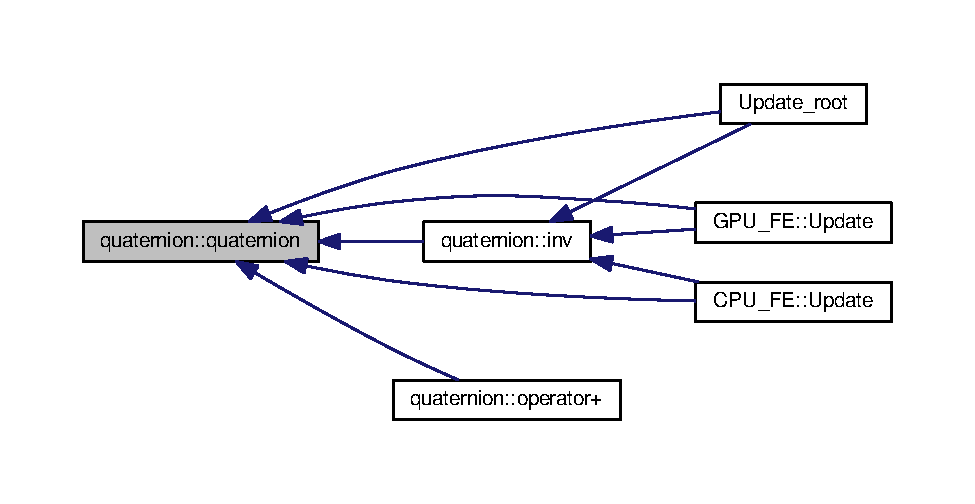
\includegraphics[width=350pt]{classquaternion_a01adb7930c2003b777cb91a7182c482e_icgraph}
\end{center}
\end{figure}


\index{quaternion@{quaternion}!quaternion@{quaternion}}
\index{quaternion@{quaternion}!quaternion@{quaternion}}
\paragraph[{\texorpdfstring{quaternion(float x, float y, float z, float w)}{quaternion(float x, float y, float z, float w)}}]{\setlength{\rightskip}{0pt plus 5cm}quaternion\+::quaternion (
\begin{DoxyParamCaption}
\item[{float}]{x, }
\item[{float}]{y, }
\item[{float}]{z, }
\item[{float}]{w}
\end{DoxyParamCaption}
)\hspace{0.3cm}{\ttfamily [inline]}}\hypertarget{classquaternion_a7939abaec2de1b11ff2208cbd8fbd93e}{}\label{classquaternion_a7939abaec2de1b11ff2208cbd8fbd93e}


Constructor taking x, y, z, w in order. 

Note\+: This is the only constructor provided. 
\begin{DoxyParams}{Parameters}
{\em Components} & $\textit{i}$, $\textit{j}$, $\textit{k}$, and $\mathbb{R}$ \\
\hline
\end{DoxyParams}


Definition at line \hyperlink{Voxel_8hpp_source_l00057}{57} of file \hyperlink{Voxel_8hpp_source}{Voxel.\+hpp}.



\subsubsection{Member Function Documentation}
\index{quaternion@{quaternion}!inv@{inv}}
\index{inv@{inv}!quaternion@{quaternion}}
\paragraph[{\texorpdfstring{inv()}{inv()}}]{\setlength{\rightskip}{0pt plus 5cm}{\bf quaternion} quaternion\+::inv (
\begin{DoxyParamCaption}
{}
\end{DoxyParamCaption}
)\hspace{0.3cm}{\ttfamily [inline]}}\hypertarget{classquaternion_a52cd9cd03bc2613e56dd798cb1037a51}{}\label{classquaternion_a52cd9cd03bc2613e56dd798cb1037a51}


Inverse of the quaternion. 

To be used as q.\+inv() $\equiv q^{-1}$ \begin{DoxyReturn}{Returns}
quaternion 
\end{DoxyReturn}


Definition at line \hyperlink{Voxel_8hpp_source_l00068}{68} of file \hyperlink{Voxel_8hpp_source}{Voxel.\+hpp}.



Here is the call graph for this function\+:\nopagebreak
\begin{figure}[H]
\begin{center}
\leavevmode
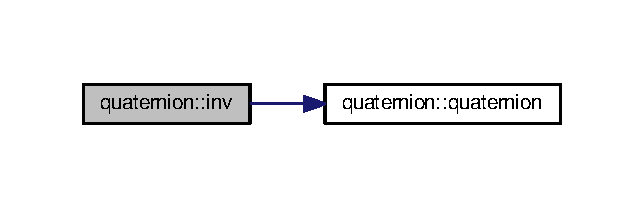
\includegraphics[width=309pt]{classquaternion_a52cd9cd03bc2613e56dd798cb1037a51_cgraph}
\end{center}
\end{figure}


\index{quaternion@{quaternion}!inv@{inv}}
\index{inv@{inv}!quaternion@{quaternion}}
\paragraph[{\texorpdfstring{inv()}{inv()}}]{\setlength{\rightskip}{0pt plus 5cm}\+\_\+\+\_\+host\+\_\+\+\_\+ \+\_\+\+\_\+device\+\_\+\+\_\+ {\bf quaternion} quaternion\+::inv (
\begin{DoxyParamCaption}
{}
\end{DoxyParamCaption}
)\hspace{0.3cm}{\ttfamily [inline]}}\hypertarget{classquaternion_a5f2dff4e0f446d05e826a63d5a45d230}{}\label{classquaternion_a5f2dff4e0f446d05e826a63d5a45d230}


Inverse of the quaternion. 

To be used as q.\+inv() $\equiv q^{-1}$ \begin{DoxyReturn}{Returns}
quaternion 
\end{DoxyReturn}


Definition at line \hyperlink{Voxel_8cuh_source_l00088}{88} of file \hyperlink{Voxel_8cuh_source}{Voxel.\+cuh}.



Here is the call graph for this function\+:\nopagebreak
\begin{figure}[H]
\begin{center}
\leavevmode
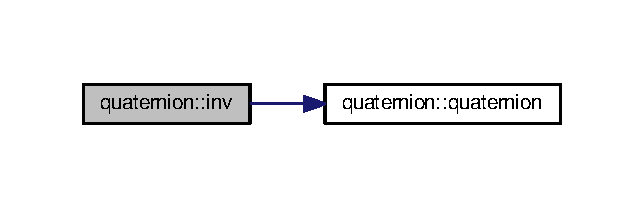
\includegraphics[width=309pt]{classquaternion_a5f2dff4e0f446d05e826a63d5a45d230_cgraph}
\end{center}
\end{figure}




Here is the caller graph for this function\+:\nopagebreak
\begin{figure}[H]
\begin{center}
\leavevmode
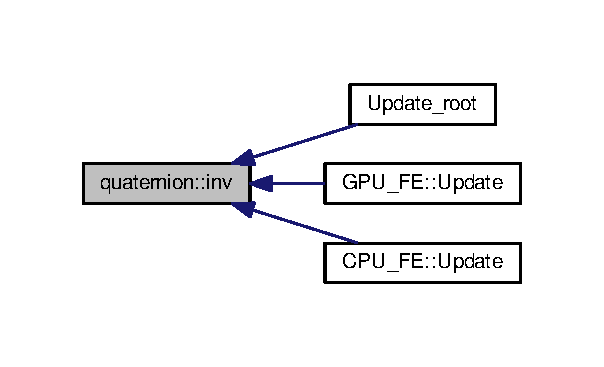
\includegraphics[width=290pt]{classquaternion_a5f2dff4e0f446d05e826a63d5a45d230_icgraph}
\end{center}
\end{figure}


\index{quaternion@{quaternion}!operator$\ast$@{operator$\ast$}}
\index{operator$\ast$@{operator$\ast$}!quaternion@{quaternion}}
\paragraph[{\texorpdfstring{operator$\ast$(quaternion const \&q)}{operator*(quaternion const &q)}}]{\setlength{\rightskip}{0pt plus 5cm}{\bf quaternion} quaternion\+::operator$\ast$ (
\begin{DoxyParamCaption}
\item[{{\bf quaternion} const \&}]{q}
\end{DoxyParamCaption}
)\hspace{0.3cm}{\ttfamily [inline]}}\hypertarget{classquaternion_a444a0e12b77a4388d496de9210117786}{}\label{classquaternion_a444a0e12b77a4388d496de9210117786}


$\times$ operator 



Definition at line \hyperlink{Voxel_8hpp_source_l00078}{78} of file \hyperlink{Voxel_8hpp_source}{Voxel.\+hpp}.

\index{quaternion@{quaternion}!operator$\ast$@{operator$\ast$}}
\index{operator$\ast$@{operator$\ast$}!quaternion@{quaternion}}
\paragraph[{\texorpdfstring{operator$\ast$(quaternion const \&q)}{operator*(quaternion const &q)}}]{\setlength{\rightskip}{0pt plus 5cm}\+\_\+\+\_\+host\+\_\+\+\_\+ \+\_\+\+\_\+device\+\_\+\+\_\+ {\bf quaternion} quaternion\+::operator$\ast$ (
\begin{DoxyParamCaption}
\item[{{\bf quaternion} const \&}]{q}
\end{DoxyParamCaption}
)\hspace{0.3cm}{\ttfamily [inline]}}\hypertarget{classquaternion_a63777bf9c0c0a269852808442c2be4f5}{}\label{classquaternion_a63777bf9c0c0a269852808442c2be4f5}


$\times$ operator 



Definition at line \hyperlink{Voxel_8cuh_source_l00098}{98} of file \hyperlink{Voxel_8cuh_source}{Voxel.\+cuh}.

\index{quaternion@{quaternion}!operator+@{operator+}}
\index{operator+@{operator+}!quaternion@{quaternion}}
\paragraph[{\texorpdfstring{operator+(quaternion const \&q)}{operator+(quaternion const &q)}}]{\setlength{\rightskip}{0pt plus 5cm}{\bf quaternion} quaternion\+::operator+ (
\begin{DoxyParamCaption}
\item[{{\bf quaternion} const \&}]{q}
\end{DoxyParamCaption}
)\hspace{0.3cm}{\ttfamily [inline]}}\hypertarget{classquaternion_a5def90b88f02a02961ff51d6cd3e7dae}{}\label{classquaternion_a5def90b88f02a02961ff51d6cd3e7dae}


$+$ operator 



Definition at line \hyperlink{Voxel_8hpp_source_l00092}{92} of file \hyperlink{Voxel_8hpp_source}{Voxel.\+hpp}.



Here is the call graph for this function\+:\nopagebreak
\begin{figure}[H]
\begin{center}
\leavevmode
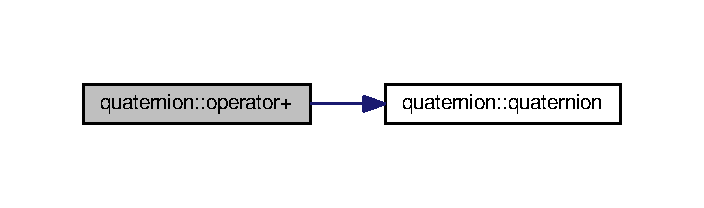
\includegraphics[width=338pt]{classquaternion_a5def90b88f02a02961ff51d6cd3e7dae_cgraph}
\end{center}
\end{figure}


\index{quaternion@{quaternion}!operator+@{operator+}}
\index{operator+@{operator+}!quaternion@{quaternion}}
\paragraph[{\texorpdfstring{operator+(quaternion const \&q)}{operator+(quaternion const &q)}}]{\setlength{\rightskip}{0pt plus 5cm}\+\_\+\+\_\+host\+\_\+\+\_\+ \+\_\+\+\_\+device\+\_\+\+\_\+ {\bf quaternion} quaternion\+::operator+ (
\begin{DoxyParamCaption}
\item[{{\bf quaternion} const \&}]{q}
\end{DoxyParamCaption}
)\hspace{0.3cm}{\ttfamily [inline]}}\hypertarget{classquaternion_ae2cf533c781610bf66bf39c30bd6b6ec}{}\label{classquaternion_ae2cf533c781610bf66bf39c30bd6b6ec}


$+$ operator 



Definition at line \hyperlink{Voxel_8cuh_source_l00112}{112} of file \hyperlink{Voxel_8cuh_source}{Voxel.\+cuh}.



Here is the call graph for this function\+:\nopagebreak
\begin{figure}[H]
\begin{center}
\leavevmode
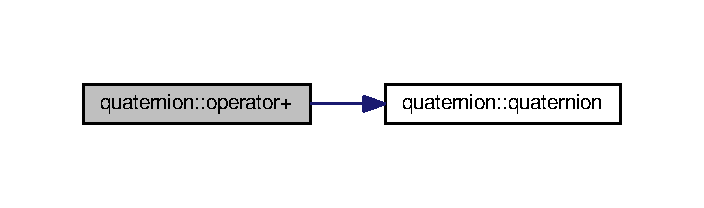
\includegraphics[width=338pt]{classquaternion_ae2cf533c781610bf66bf39c30bd6b6ec_cgraph}
\end{center}
\end{figure}




\subsubsection{Member Data Documentation}
\index{quaternion@{quaternion}!w@{w}}
\index{w@{w}!quaternion@{quaternion}}
\paragraph[{\texorpdfstring{w}{w}}]{\setlength{\rightskip}{0pt plus 5cm}float quaternion\+::w}\hypertarget{classquaternion_ab2b38aca1971114e0ba4218b75d7f472}{}\label{classquaternion_ab2b38aca1971114e0ba4218b75d7f472}


Definition at line \hyperlink{Voxel_8cuh_source_l00069}{69} of file \hyperlink{Voxel_8cuh_source}{Voxel.\+cuh}.

\index{quaternion@{quaternion}!x@{x}}
\index{x@{x}!quaternion@{quaternion}}
\paragraph[{\texorpdfstring{x}{x}}]{\setlength{\rightskip}{0pt plus 5cm}float quaternion\+::x}\hypertarget{classquaternion_acdcda48f9dd7ff35873aae38fa33ab78}{}\label{classquaternion_acdcda48f9dd7ff35873aae38fa33ab78}


Definition at line \hyperlink{Voxel_8cuh_source_l00069}{69} of file \hyperlink{Voxel_8cuh_source}{Voxel.\+cuh}.

\index{quaternion@{quaternion}!y@{y}}
\index{y@{y}!quaternion@{quaternion}}
\paragraph[{\texorpdfstring{y}{y}}]{\setlength{\rightskip}{0pt plus 5cm}float quaternion\+::y}\hypertarget{classquaternion_a48e3d1fbf5e12eb54985c32b45dd8303}{}\label{classquaternion_a48e3d1fbf5e12eb54985c32b45dd8303}


Definition at line \hyperlink{Voxel_8cuh_source_l00069}{69} of file \hyperlink{Voxel_8cuh_source}{Voxel.\+cuh}.

\index{quaternion@{quaternion}!z@{z}}
\index{z@{z}!quaternion@{quaternion}}
\paragraph[{\texorpdfstring{z}{z}}]{\setlength{\rightskip}{0pt plus 5cm}float quaternion\+::z}\hypertarget{classquaternion_a538598007238d399f79ddcecd39ef5cf}{}\label{classquaternion_a538598007238d399f79ddcecd39ef5cf}


Definition at line \hyperlink{Voxel_8cuh_source_l00069}{69} of file \hyperlink{Voxel_8cuh_source}{Voxel.\+cuh}.



The documentation for this class was generated from the following files\+:\begin{DoxyCompactItemize}
\item 
include/\hyperlink{Voxel_8cuh}{Voxel.\+cuh}\item 
include/\hyperlink{Voxel_8hpp}{Voxel.\+hpp}\end{DoxyCompactItemize}

\hypertarget{structTuple}{}\subsection{Tuple Struct Reference}
\label{structTuple}\index{Tuple@{Tuple}}


Point co-\/ordinates and variance  


\subsubsection*{Public Attributes}
\begin{Indent}{\bf Point co-\/ordinates}\par
\begin{DoxyCompactItemize}
\item 
float \hyperlink{structTuple_a9355c336c18afa6b76685ddffe16c5a5}{x}
\item 
float \hyperlink{structTuple_ae298b0277eb33e02696b6e3716e93c46}{y}
\item 
float \hyperlink{structTuple_a5f83aeb6b110bc956fd27b8e713a9ad5}{z}
\end{DoxyCompactItemize}
\end{Indent}
\begin{Indent}{\bf Variance}\par
\begin{DoxyCompactItemize}
\item 
float \hyperlink{structTuple_a69871fb52122a48baa140565fb1b7c0c}{c}
\end{DoxyCompactItemize}
\end{Indent}


\subsubsection{Detailed Description}
Point co-\/ordinates and variance 

Used to pass to C\+U\+DA kernel 

Definition at line \hyperlink{Voxel_8cuh_source_l00157}{157} of file \hyperlink{Voxel_8cuh_source}{Voxel.\+cuh}.



\subsubsection{Member Data Documentation}
\index{Tuple@{Tuple}!c@{c}}
\index{c@{c}!Tuple@{Tuple}}
\paragraph[{\texorpdfstring{c}{c}}]{\setlength{\rightskip}{0pt plus 5cm}float Tuple\+::c}\hypertarget{structTuple_a69871fb52122a48baa140565fb1b7c0c}{}\label{structTuple_a69871fb52122a48baa140565fb1b7c0c}


Definition at line \hyperlink{Voxel_8cuh_source_l00166}{166} of file \hyperlink{Voxel_8cuh_source}{Voxel.\+cuh}.

\index{Tuple@{Tuple}!x@{x}}
\index{x@{x}!Tuple@{Tuple}}
\paragraph[{\texorpdfstring{x}{x}}]{\setlength{\rightskip}{0pt plus 5cm}float Tuple\+::x}\hypertarget{structTuple_a9355c336c18afa6b76685ddffe16c5a5}{}\label{structTuple_a9355c336c18afa6b76685ddffe16c5a5}


Definition at line \hyperlink{Voxel_8cuh_source_l00162}{162} of file \hyperlink{Voxel_8cuh_source}{Voxel.\+cuh}.

\index{Tuple@{Tuple}!y@{y}}
\index{y@{y}!Tuple@{Tuple}}
\paragraph[{\texorpdfstring{y}{y}}]{\setlength{\rightskip}{0pt plus 5cm}float Tuple\+::y}\hypertarget{structTuple_ae298b0277eb33e02696b6e3716e93c46}{}\label{structTuple_ae298b0277eb33e02696b6e3716e93c46}


Definition at line \hyperlink{Voxel_8cuh_source_l00162}{162} of file \hyperlink{Voxel_8cuh_source}{Voxel.\+cuh}.

\index{Tuple@{Tuple}!z@{z}}
\index{z@{z}!Tuple@{Tuple}}
\paragraph[{\texorpdfstring{z}{z}}]{\setlength{\rightskip}{0pt plus 5cm}float Tuple\+::z}\hypertarget{structTuple_a5f83aeb6b110bc956fd27b8e713a9ad5}{}\label{structTuple_a5f83aeb6b110bc956fd27b8e713a9ad5}


Definition at line \hyperlink{Voxel_8cuh_source_l00162}{162} of file \hyperlink{Voxel_8cuh_source}{Voxel.\+cuh}.



The documentation for this struct was generated from the following file\+:\begin{DoxyCompactItemize}
\item 
include/\hyperlink{Voxel_8cuh}{Voxel.\+cuh}\end{DoxyCompactItemize}

\hypertarget{classvoxel}{}\subsection{voxel Class Reference}
\label{classvoxel}\index{voxel@{voxel}}


Voxel/\+Intermediate nodes of the Octree structure.  




{\ttfamily \#include $<$Voxel.\+hpp$>$}

\subsubsection*{Public Member Functions}
\begin{DoxyCompactItemize}
\item 
\+\_\+\+\_\+device\+\_\+\+\_\+ \hyperlink{classvoxel_a1f832fd40f23c4fd721a4144387db6ef}{voxel} (float x, float y, float z, float \hyperlink{classvoxel_a573bae3d6e8383a4b2235d3cd33e7ab6}{size})
\begin{DoxyCompactList}\small\item\em Constructor for voxel node. \end{DoxyCompactList}\item 
\+\_\+\+\_\+device\+\_\+\+\_\+ void \hyperlink{classvoxel_a97737aec7c381e72d929d2f084952683}{update\+\_\+vox} (float x, float y, float z)
\begin{DoxyCompactList}\small\item\em Update method for this node object. \end{DoxyCompactList}\item 
\+\_\+\+\_\+device\+\_\+\+\_\+ void \hyperlink{classvoxel_a1748472909af5ef1f28d0a0c6648dbbd}{update\+\_\+self} (float x, float y, float z)
\begin{DoxyCompactList}\small\item\em Update method for self. \end{DoxyCompactList}\item 
\+\_\+\+\_\+device\+\_\+\+\_\+ void \hyperlink{classvoxel_aff25abf72186eb31821d1ffacf557c67}{free\+\_\+mem} ()
\begin{DoxyCompactList}\small\item\em Recursively frees up memory inside this voxel node. \end{DoxyCompactList}\item 
\+\_\+\+\_\+device\+\_\+\+\_\+ void \hyperlink{classvoxel_a4189fb0f24ad9eba1447e2ebf8ee0015}{all\+\_\+points} (\hyperlink{structTuple}{Tuple} $\ast$set, float x\+\_\+o, float y\+\_\+o, float z\+\_\+o, int $\ast$idx)
\begin{DoxyCompactList}\small\item\em Appends all leaf node points in this node to vector set. \end{DoxyCompactList}\item 
\+\_\+\+\_\+device\+\_\+\+\_\+ bool \hyperlink{classvoxel_ae8d08bec6f007a905812764672327522}{is\+\_\+empty} ()
\begin{DoxyCompactList}\small\item\em Checks if this node has been observed or not. \end{DoxyCompactList}\item 
\hyperlink{classvoxel_a77f20a6fddec8f3aa3c719c3dc609948}{voxel} (float x, float y, float z, float \hyperlink{classvoxel_a573bae3d6e8383a4b2235d3cd33e7ab6}{size})
\begin{DoxyCompactList}\small\item\em Constructor for voxel node. \end{DoxyCompactList}\item 
void \hyperlink{classvoxel_ae550590cfe0d4c3d0e78cbf0cfa3390f}{update\+\_\+vox} (float x, float y, float z)
\begin{DoxyCompactList}\small\item\em Update method for this node object. \end{DoxyCompactList}\item 
void \hyperlink{classvoxel_ac766278266424ede18f1fae9ccfd88be}{free\+\_\+mem} ()
\begin{DoxyCompactList}\small\item\em Recursively frees up memory inside this voxel node. \end{DoxyCompactList}\item 
void \hyperlink{classvoxel_aaea83372a2e28b25ae65dcc635ebe635}{all\+\_\+points} (std\+::vector$<$ std\+::tuple$<$ float, float, float, float $>$ $>$ $\ast$set, float x\+\_\+o, float y\+\_\+o, float z\+\_\+o)
\begin{DoxyCompactList}\small\item\em Appends all leaf node points in this node to vector set. \end{DoxyCompactList}\item 
bool \hyperlink{classvoxel_afe0d1d928ee0358b0fc0a67f58793cfd}{is\+\_\+empty} ()
\begin{DoxyCompactList}\small\item\em Checks if this node has been observed or not. \end{DoxyCompactList}\end{DoxyCompactItemize}
\subsubsection*{Public Attributes}
\begin{DoxyCompactItemize}
\item 
void $\ast$ \hyperlink{classvoxel_aa280f71c0258d85ffef6f1818872a00a}{c} \mbox{[}8\mbox{]}
\begin{DoxyCompactList}\small\item\em Pointers to child voxels/leafs. \end{DoxyCompactList}\item 
float \hyperlink{classvoxel_a01aebb82be393552c039c11a2c168845}{\+\_\+v}
\begin{DoxyCompactList}\small\item\em Inverse of variance. \end{DoxyCompactList}\item 
float \hyperlink{classvoxel_a573bae3d6e8383a4b2235d3cd33e7ab6}{size}
\end{DoxyCompactItemize}
\begin{Indent}{\bf Co-\/ordinates}\par
{\em Co-\/ordinates of a single point inside voxel node divided by the variance.

The co-\/ordinates are measured relative to voxel node edge length, ie. $x, y, z \in [0,1)$. Note that although x\+\_\+v, y\+\_\+v, and z\+\_\+v can are unbounded, the values of x, y, and z are bounded since the update is a convex combination of two points inside the node. The co-\/ordinates are divided by the variance so that the update can be performed in a single atomic operation while running in G\+PU. \begin{DoxySeeAlso}{See also}
\hyperlink{Voxel_8cuh}{Voxel.\+cuh} 
\end{DoxySeeAlso}
}\begin{DoxyCompactItemize}
\item 
float \hyperlink{classvoxel_a263a7912d9018052399d4b99fb220f2e}{x\+\_\+v}
\item 
float \hyperlink{classvoxel_a67b339eef4ce4330a18d15973dcf6a24}{y\+\_\+v}
\item 
float \hyperlink{classvoxel_a66addb3e42303e4a90a745c2174b0043}{z\+\_\+v}
\end{DoxyCompactItemize}
\end{Indent}


\subsubsection{Detailed Description}
Voxel/\+Intermediate nodes of the Octree structure. 

G\+PU\+: ~\newline
 Primarily stores the pointers to the eight children of this voxel object. Additionally it also stores the co-\/ordinate of a combined single point, calculated from all its children. This information can be used if memory consumed by the Octree structure reaches a threshold, in which case all the children of a voxel object at some particular level can deleted freeing some space, but at the same time not losing information about the space inside (although accuracy will decrease). The x, y, z co-\/ordinates of thr single point stored inside is relative to edge length ie. $x, y, z \in [0,1)$. This is to maintain uniform accuracy across all points. (accuracy of float type reduces as one moves away from 0) The origin of the node is the vertex with all co-\/ordinates minimum. ie. if the origin of voxel is $(x_o, y_o, z_o)$ and edge length is $L$, The vertices of the node are $\{(x_o, y_o, z_o), ..., (x_o+L, y_o+L, z_o+L)\}$ If the member \hyperlink{classvoxel_a01aebb82be393552c039c11a2c168845}{voxel\+::\+\_\+v} $> 0$, the leaf node is occupied. If \+\_\+v $= 0$, the voxel node is empty (this is not the same as unobserved. This means that this node has been observed, but there is no point inside it). This has been used becuase if initially a node was observed to be empty, and containing a point afterwards, the same update rule can be used without any change, in a single atomic operation. Additionally, if any child pointer c\mbox{[}i\mbox{]} $= NULL$, then that child has not yet been observed. An object of this class can only be declared inside the C\+U\+DA kernel.

C\+PU\+: ~\newline
 Primarily stores the pointers to the eight children of this voxel object. Additionally it also stores the co-\/ordinate of a combined single point, calculated from all its children. This information can be used if memory consumed by the Octree structure reaches a threshold, in which case all the children of a voxel object at some particular level can deleted freeing some space, but at the same time not losing information about the space inside (although accuracy will decrease). The x, y, z co-\/ordinates of thr single point stored inside is relative to edge length ie. $x, y, z \in [0,1)$. This is to maintain uniform accuracy across all points. (accuracy of float type reduces as one moves away from 0) The origin of the node is the vertex with all co-\/ordinates minimum. ie. if the origin of voxel is $(x_o, y_o, z_o)$ and edge length is $L$, The vertices of the node are $\{(x_o, y_o, z_o), ..., (x_o+L, y_o+L, z_o+L)\}$ If the member \hyperlink{classvoxel_a01aebb82be393552c039c11a2c168845}{voxel\+::\+\_\+v} $> 0$, the leaf node is occupied. If \+\_\+v $= 0$, the voxel node is empty (this is not the same as unobserved. This means that this node has been observed, but there is no point inside it). This has been used becuase if initially a node was observed to be empty, and containing a point afterwards, the same update rule can be used without any change, in a single atomic operation. Additionally, if any child pointer c\mbox{[}i\mbox{]} $= NULL$, then that child has not yet been observed. 

Definition at line \hyperlink{Voxel_8cuh_source_l00297}{297} of file \hyperlink{Voxel_8cuh_source}{Voxel.\+cuh}.



\subsubsection{Constructor \& Destructor Documentation}
\index{voxel@{voxel}!voxel@{voxel}}
\index{voxel@{voxel}!voxel@{voxel}}
\paragraph[{\texorpdfstring{voxel(float x, float y, float z, float size)}{voxel(float x, float y, float z, float size)}}]{\setlength{\rightskip}{0pt plus 5cm}\+\_\+\+\_\+device\+\_\+\+\_\+ voxel\+::voxel (
\begin{DoxyParamCaption}
\item[{float}]{x, }
\item[{float}]{y, }
\item[{float}]{z, }
\item[{float}]{size}
\end{DoxyParamCaption}
)\hspace{0.3cm}{\ttfamily [inline]}}\hypertarget{classvoxel_a1f832fd40f23c4fd721a4144387db6ef}{}\label{classvoxel_a1f832fd40f23c4fd721a4144387db6ef}


Constructor for voxel node. 

Note that this is the only constructor provided. 
\begin{DoxyParams}{Parameters}
{\em (x,y,z)} & relative to node, ie. $x, y, z \in [0,1)$ for correct operation \\
\hline
{\em edge} & length of voxel ( $\textit{m}$) \\
\hline
\end{DoxyParams}


Definition at line \hyperlink{Voxel_8cuh_source_l00334}{334} of file \hyperlink{Voxel_8cuh_source}{Voxel.\+cuh}.

\index{voxel@{voxel}!voxel@{voxel}}
\index{voxel@{voxel}!voxel@{voxel}}
\paragraph[{\texorpdfstring{voxel(float x, float y, float z, float size)}{voxel(float x, float y, float z, float size)}}]{\setlength{\rightskip}{0pt plus 5cm}voxel\+::voxel (
\begin{DoxyParamCaption}
\item[{float}]{x, }
\item[{float}]{y, }
\item[{float}]{z, }
\item[{float}]{size}
\end{DoxyParamCaption}
)\hspace{0.3cm}{\ttfamily [inline]}}\hypertarget{classvoxel_a77f20a6fddec8f3aa3c719c3dc609948}{}\label{classvoxel_a77f20a6fddec8f3aa3c719c3dc609948}


Constructor for voxel node. 

Note that this is the only constructor provided. If the parameters provided are $(-1, -1, -,1)$, the node is set to be empty. Note that x\+\_\+v, y\+\_\+v, and z\+\_\+v are set $= 0$. 
\begin{DoxyParams}{Parameters}
{\em (x,y,z)} & relative to node, ie. $x, y, z \in [0,1)$ for correct operation \\
\hline
{\em edge} & length of voxel ( $\textit{m}$) \\
\hline
\end{DoxyParams}


Definition at line \hyperlink{Voxel_8hpp_source_l00236}{236} of file \hyperlink{Voxel_8hpp_source}{Voxel.\+hpp}.



\subsubsection{Member Function Documentation}
\index{voxel@{voxel}!all\+\_\+points@{all\+\_\+points}}
\index{all\+\_\+points@{all\+\_\+points}!voxel@{voxel}}
\paragraph[{\texorpdfstring{all\+\_\+points(std\+::vector$<$ std\+::tuple$<$ float, float, float, float $>$ $>$ $\ast$set, float x\+\_\+o, float y\+\_\+o, float z\+\_\+o)}{all_points(std::vector< std::tuple< float, float, float, float > > *set, float x_o, float y_o, float z_o)}}]{\setlength{\rightskip}{0pt plus 5cm}void voxel\+::all\+\_\+points (
\begin{DoxyParamCaption}
\item[{std\+::vector$<$ std\+::tuple$<$ float, float, float, float $>$ $>$ $\ast$}]{set, }
\item[{float}]{x\+\_\+o, }
\item[{float}]{y\+\_\+o, }
\item[{float}]{z\+\_\+o}
\end{DoxyParamCaption}
)\hspace{0.3cm}{\ttfamily [inline]}}\hypertarget{classvoxel_aaea83372a2e28b25ae65dcc635ebe635}{}\label{classvoxel_aaea83372a2e28b25ae65dcc635ebe635}


Appends all leaf node points in this node to vector set. 



Definition at line \hyperlink{Voxel_8hpp_source_l00310}{310} of file \hyperlink{Voxel_8hpp_source}{Voxel.\+hpp}.

\index{voxel@{voxel}!all\+\_\+points@{all\+\_\+points}}
\index{all\+\_\+points@{all\+\_\+points}!voxel@{voxel}}
\paragraph[{\texorpdfstring{all\+\_\+points(\+Tuple $\ast$set, float x\+\_\+o, float y\+\_\+o, float z\+\_\+o, int $\ast$idx)}{all_points(Tuple *set, float x_o, float y_o, float z_o, int *idx)}}]{\setlength{\rightskip}{0pt plus 5cm}\+\_\+\+\_\+device\+\_\+\+\_\+ void voxel\+::all\+\_\+points (
\begin{DoxyParamCaption}
\item[{{\bf Tuple} $\ast$}]{set, }
\item[{float}]{x\+\_\+o, }
\item[{float}]{y\+\_\+o, }
\item[{float}]{z\+\_\+o, }
\item[{int $\ast$}]{idx}
\end{DoxyParamCaption}
)\hspace{0.3cm}{\ttfamily [inline]}}\hypertarget{classvoxel_a4189fb0f24ad9eba1447e2ebf8ee0015}{}\label{classvoxel_a4189fb0f24ad9eba1447e2ebf8ee0015}


Appends all leaf node points in this node to vector set. 



Definition at line \hyperlink{Voxel_8cuh_source_l00432}{432} of file \hyperlink{Voxel_8cuh_source}{Voxel.\+cuh}.

\index{voxel@{voxel}!free\+\_\+mem@{free\+\_\+mem}}
\index{free\+\_\+mem@{free\+\_\+mem}!voxel@{voxel}}
\paragraph[{\texorpdfstring{free\+\_\+mem()}{free_mem()}}]{\setlength{\rightskip}{0pt plus 5cm}void voxel\+::free\+\_\+mem (
\begin{DoxyParamCaption}
{}
\end{DoxyParamCaption}
)\hspace{0.3cm}{\ttfamily [inline]}}\hypertarget{classvoxel_ac766278266424ede18f1fae9ccfd88be}{}\label{classvoxel_ac766278266424ede18f1fae9ccfd88be}


Recursively frees up memory inside this voxel node. 

This is called upon by the member method \hyperlink{classocc__grid_adbfab59a1fb247d53a993fd9a2a26d67}{occ\+\_\+grid\+::free\+\_\+mem()} (which is inturn called by \hyperlink{classCPU__FE_a425dc3014e22d7aeaaf261ac945f4da1}{C\+P\+U\+\_\+\+F\+E\+::$\sim$\+C\+P\+U\+\_\+\+F\+E()}) on each of the root voxel nodes, which recursively deletes all the nodes in the octree. \begin{DoxySeeAlso}{See also}
\hyperlink{classocc__grid_adbfab59a1fb247d53a993fd9a2a26d67}{occ\+\_\+grid\+::free\+\_\+mem()}, \hyperlink{classCPU__FE_a425dc3014e22d7aeaaf261ac945f4da1}{C\+P\+U\+\_\+\+F\+E\+::$\sim$\+C\+P\+U\+\_\+\+F\+E()} 
\end{DoxySeeAlso}


Definition at line \hyperlink{Voxel_8hpp_source_l00286}{286} of file \hyperlink{Voxel_8hpp_source}{Voxel.\+hpp}.

\index{voxel@{voxel}!free\+\_\+mem@{free\+\_\+mem}}
\index{free\+\_\+mem@{free\+\_\+mem}!voxel@{voxel}}
\paragraph[{\texorpdfstring{free\+\_\+mem()}{free_mem()}}]{\setlength{\rightskip}{0pt plus 5cm}\+\_\+\+\_\+device\+\_\+\+\_\+ void voxel\+::free\+\_\+mem (
\begin{DoxyParamCaption}
{}
\end{DoxyParamCaption}
)\hspace{0.3cm}{\ttfamily [inline]}}\hypertarget{classvoxel_aff25abf72186eb31821d1ffacf557c67}{}\label{classvoxel_aff25abf72186eb31821d1ffacf557c67}


Recursively frees up memory inside this voxel node. 

This is called upon by the global method Delete() (which is inturn called by \hyperlink{classGPU__FE_a1da80fa2f9f13df184e545e46f9d9270}{G\+P\+U\+\_\+\+F\+E\+::$\sim$\+G\+P\+U\+\_\+\+F\+E()}) on each of the root voxel nodes, which recursively deletes all the nodes in the octree. Run by a single C\+U\+DA thread, since it is called only once and doesn\textquotesingle{}t affect the performance. \begin{DoxySeeAlso}{See also}
\hyperlink{classGPU__FE_a1da80fa2f9f13df184e545e46f9d9270}{G\+P\+U\+\_\+\+F\+E\+::$\sim$\+G\+P\+U\+\_\+\+F\+E()}, Delete() 
\end{DoxySeeAlso}


Definition at line \hyperlink{Voxel_8cuh_source_l00407}{407} of file \hyperlink{Voxel_8cuh_source}{Voxel.\+cuh}.

\index{voxel@{voxel}!is\+\_\+empty@{is\+\_\+empty}}
\index{is\+\_\+empty@{is\+\_\+empty}!voxel@{voxel}}
\paragraph[{\texorpdfstring{is\+\_\+empty()}{is_empty()}}]{\setlength{\rightskip}{0pt plus 5cm}bool voxel\+::is\+\_\+empty (
\begin{DoxyParamCaption}
{}
\end{DoxyParamCaption}
)\hspace{0.3cm}{\ttfamily [inline]}}\hypertarget{classvoxel_afe0d1d928ee0358b0fc0a67f58793cfd}{}\label{classvoxel_afe0d1d928ee0358b0fc0a67f58793cfd}


Checks if this node has been observed or not. 

If the node has atleast one filled or empty children, this method returns false. \begin{DoxySeeAlso}{See also}
\hyperlink{classvoxel}{voxel} 
\end{DoxySeeAlso}


Definition at line \hyperlink{Voxel_8hpp_source_l00333}{333} of file \hyperlink{Voxel_8hpp_source}{Voxel.\+hpp}.

\index{voxel@{voxel}!is\+\_\+empty@{is\+\_\+empty}}
\index{is\+\_\+empty@{is\+\_\+empty}!voxel@{voxel}}
\paragraph[{\texorpdfstring{is\+\_\+empty()}{is_empty()}}]{\setlength{\rightskip}{0pt plus 5cm}\+\_\+\+\_\+device\+\_\+\+\_\+ bool voxel\+::is\+\_\+empty (
\begin{DoxyParamCaption}
{}
\end{DoxyParamCaption}
)\hspace{0.3cm}{\ttfamily [inline]}}\hypertarget{classvoxel_ae8d08bec6f007a905812764672327522}{}\label{classvoxel_ae8d08bec6f007a905812764672327522}


Checks if this node has been observed or not. 

If the node has atleast one filled or empty children, this method returns false. \begin{DoxySeeAlso}{See also}
\hyperlink{classvoxel}{voxel} 
\end{DoxySeeAlso}


Definition at line \hyperlink{Voxel_8cuh_source_l00456}{456} of file \hyperlink{Voxel_8cuh_source}{Voxel.\+cuh}.

\index{voxel@{voxel}!update\+\_\+self@{update\+\_\+self}}
\index{update\+\_\+self@{update\+\_\+self}!voxel@{voxel}}
\paragraph[{\texorpdfstring{update\+\_\+self(float x, float y, float z)}{update_self(float x, float y, float z)}}]{\setlength{\rightskip}{0pt plus 5cm}\+\_\+\+\_\+device\+\_\+\+\_\+ void voxel\+::update\+\_\+self (
\begin{DoxyParamCaption}
\item[{float}]{x, }
\item[{float}]{y, }
\item[{float}]{z}
\end{DoxyParamCaption}
)\hspace{0.3cm}{\ttfamily [inline]}}\hypertarget{classvoxel_a1748472909af5ef1f28d0a0c6648dbbd}{}\label{classvoxel_a1748472909af5ef1f28d0a0c6648dbbd}


Update method for self. 

Following the update of the children, the point stored inside this voxel is updated. atommic\+Add() function and the transformed variables ensure consistency while multi-\/threading. This method is similar to \hyperlink{classleaf_a3c205ce57e242832977bde6e1a04d7da}{leaf\+::update\+\_\+leaf()} 
\begin{DoxyParams}{Parameters}
{\em (x,y,z)} & relative to node, ie. $x, y, z \in [0,1)$ for correct operation \\
\hline
\end{DoxyParams}
\begin{DoxySeeAlso}{See also}
\hyperlink{classleaf_a3c205ce57e242832977bde6e1a04d7da}{leaf\+::update\+\_\+leaf()}, \hyperlink{classvoxel_a97737aec7c381e72d929d2f084952683}{voxel\+::update\+\_\+vox()} 
\end{DoxySeeAlso}


Definition at line \hyperlink{Voxel_8cuh_source_l00394}{394} of file \hyperlink{Voxel_8cuh_source}{Voxel.\+cuh}.



Here is the caller graph for this function\+:\nopagebreak
\begin{figure}[H]
\begin{center}
\leavevmode
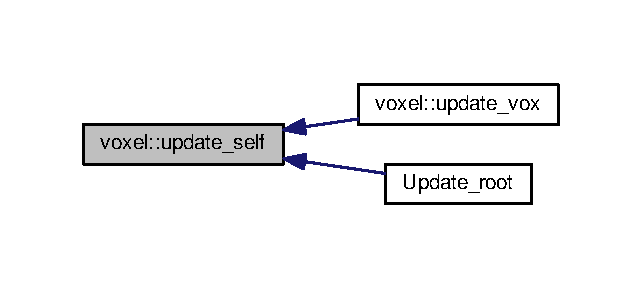
\includegraphics[width=308pt]{classvoxel_a1748472909af5ef1f28d0a0c6648dbbd_icgraph}
\end{center}
\end{figure}


\index{voxel@{voxel}!update\+\_\+vox@{update\+\_\+vox}}
\index{update\+\_\+vox@{update\+\_\+vox}!voxel@{voxel}}
\paragraph[{\texorpdfstring{update\+\_\+vox(float x, float y, float z)}{update_vox(float x, float y, float z)}}]{\setlength{\rightskip}{0pt plus 5cm}void voxel\+::update\+\_\+vox (
\begin{DoxyParamCaption}
\item[{float}]{x, }
\item[{float}]{y, }
\item[{float}]{z}
\end{DoxyParamCaption}
)\hspace{0.3cm}{\ttfamily [inline]}}\hypertarget{classvoxel_ae550590cfe0d4c3d0e78cbf0cfa3390f}{}\label{classvoxel_ae550590cfe0d4c3d0e78cbf0cfa3390f}


Update method for this node object. 

For each voxel, two update steps are performed\+: one for the child voxel/leaf the input point lies in, and one for this voxel object. For the child update, it is first checked whether the child exists. If it does, \hyperlink{classleaf_a3c205ce57e242832977bde6e1a04d7da}{leaf\+::update\+\_\+leaf()} or \hyperlink{classvoxel_a97737aec7c381e72d929d2f084952683}{voxel\+::update\+\_\+vox()} is called on the child object. If it doesn\textquotesingle{}t, a new child voxel/leaf is created and the constructor \hyperlink{classleaf_adfaf04cd4b50545cbc902d1aa36bc609}{leaf\+::leaf()} or \hyperlink{classvoxel_a1f832fd40f23c4fd721a4144387db6ef}{voxel\+::voxel()} is called. This step is a recursive one. The decision of whether the child is a voxel node or a leaf node is made considering the edge lengths of the children. ( $=\frac{this\to\_v}{2}$) If child edge length $ \leq $ M\+I\+N\+\_\+L, the child is a leaf node, else it is a voxel node. The next step is self update which is similar to \hyperlink{classleaf_a3c205ce57e242832977bde6e1a04d7da}{leaf\+::update\+\_\+leaf()} 
\begin{DoxyParams}{Parameters}
{\em (x,y,z)} & relative to node, ie. $x, y, z \in [0,1)$ for correct operation \\
\hline
\end{DoxyParams}
\begin{DoxySeeAlso}{See also}
\hyperlink{classleaf_a3c205ce57e242832977bde6e1a04d7da}{leaf\+::update\+\_\+leaf()} 
\end{DoxySeeAlso}


Definition at line \hyperlink{Voxel_8hpp_source_l00256}{256} of file \hyperlink{Voxel_8hpp_source}{Voxel.\+hpp}.

\index{voxel@{voxel}!update\+\_\+vox@{update\+\_\+vox}}
\index{update\+\_\+vox@{update\+\_\+vox}!voxel@{voxel}}
\paragraph[{\texorpdfstring{update\+\_\+vox(float x, float y, float z)}{update_vox(float x, float y, float z)}}]{\setlength{\rightskip}{0pt plus 5cm}\+\_\+\+\_\+device\+\_\+\+\_\+ void voxel\+::update\+\_\+vox (
\begin{DoxyParamCaption}
\item[{float}]{x, }
\item[{float}]{y, }
\item[{float}]{z}
\end{DoxyParamCaption}
)\hspace{0.3cm}{\ttfamily [inline]}}\hypertarget{classvoxel_a97737aec7c381e72d929d2f084952683}{}\label{classvoxel_a97737aec7c381e72d929d2f084952683}


Update method for this node object. 

For each voxel, two update steps are performed\+: one for the child voxel/leaf the input point lies in, and one for this voxel object. For the child update, it is first checked whether the child exists. If it does, \hyperlink{classleaf_a3c205ce57e242832977bde6e1a04d7da}{leaf\+::update\+\_\+leaf()} or \hyperlink{classvoxel_a97737aec7c381e72d929d2f084952683}{voxel\+::update\+\_\+vox()} is called on the child object. If it doesn\textquotesingle{}t, a new child voxel/leaf is created and the constructor \hyperlink{classleaf_adfaf04cd4b50545cbc902d1aa36bc609}{leaf\+::leaf()} or \hyperlink{classvoxel_a1f832fd40f23c4fd721a4144387db6ef}{voxel\+::voxel()} is called. This step is a recursive one. To avoid multiple threads creating inconsistent and wasteful copies of the same child node, the following strategy is used\+: Each thread creates a copy of child voxel, then an atomic Compare and Swap (atomic\+C\+A\+S()) is applied on the child pointer. Only one thread can successfully replace the pointer. This pointer is subsequently used for all updates, and the unused children are deleted. The decision of whether the child is a voxel node or a leaf node is made considering the edge lengths of the children. ( $=\frac{this\to\_v}{2}$) If child edge length $ \leq $ M\+I\+N\+\_\+L, the child is a leaf node, else it is a voxel node. The next step is self update which is similar to \hyperlink{classleaf_a3c205ce57e242832977bde6e1a04d7da}{leaf\+::update\+\_\+leaf()} 
\begin{DoxyParams}{Parameters}
{\em (x,y,z)} & relative to node, ie. $x, y, z \in [0,1)$ for correct operation \\
\hline
\end{DoxyParams}
\begin{DoxySeeAlso}{See also}
\hyperlink{classleaf_a3c205ce57e242832977bde6e1a04d7da}{leaf\+::update\+\_\+leaf()}, \hyperlink{classvoxel_a1748472909af5ef1f28d0a0c6648dbbd}{voxel\+::update\+\_\+self()} 
\end{DoxySeeAlso}


Definition at line \hyperlink{Voxel_8cuh_source_l00355}{355} of file \hyperlink{Voxel_8cuh_source}{Voxel.\+cuh}.



Here is the call graph for this function\+:\nopagebreak
\begin{figure}[H]
\begin{center}
\leavevmode
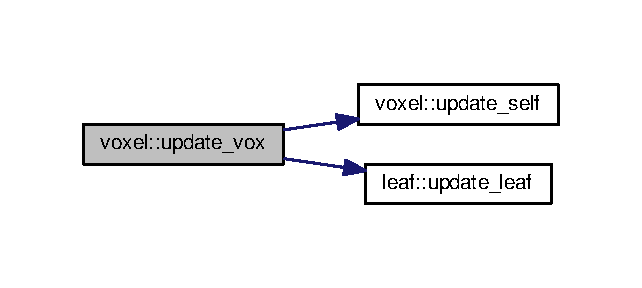
\includegraphics[width=308pt]{classvoxel_a97737aec7c381e72d929d2f084952683_cgraph}
\end{center}
\end{figure}




\subsubsection{Member Data Documentation}
\index{voxel@{voxel}!\+\_\+v@{\+\_\+v}}
\index{\+\_\+v@{\+\_\+v}!voxel@{voxel}}
\paragraph[{\texorpdfstring{\+\_\+v}{_v}}]{\setlength{\rightskip}{0pt plus 5cm}float voxel\+::\+\_\+v}\hypertarget{classvoxel_a01aebb82be393552c039c11a2c168845}{}\label{classvoxel_a01aebb82be393552c039c11a2c168845}


Inverse of variance. 

The points are assumed to be distributed as a 3-\/D uniform gaussian distribution when measured. As more points are updated in the node, this variance decreases, ie. the certainity of a point existing in the node increases. The update rule is the typical update rule of gaussian distribution, same as the one in Measurement Update Step in E\+KF and S\+L\+AM. Inverse of variance is stored so that the update can be performed in a single atomic step while running in G\+PU.

The points are assumed to be distributed as a 3-\/D uniform gaussian distribution when measured. As more points are updated in the node, this variance decreases, ie. the certainity of a point existing in the node increases. The update rule is the typical update rule of gaussian distribution, same as the one in Measurement Update Step in E\+KF and S\+L\+AM. Inverse of variance is stored so that the update can be performed in a single atomic step while running in G\+PU. \begin{DoxySeeAlso}{See also}
\hyperlink{Voxel_8cuh}{Voxel.\+cuh} 
\end{DoxySeeAlso}


Definition at line \hyperlink{Voxel_8cuh_source_l00313}{313} of file \hyperlink{Voxel_8cuh_source}{Voxel.\+cuh}.

\index{voxel@{voxel}!c@{c}}
\index{c@{c}!voxel@{voxel}}
\paragraph[{\texorpdfstring{c}{c}}]{\setlength{\rightskip}{0pt plus 5cm}void $\ast$ voxel\+::c}\hypertarget{classvoxel_aa280f71c0258d85ffef6f1818872a00a}{}\label{classvoxel_aa280f71c0258d85ffef6f1818872a00a}


Pointers to child voxels/leafs. 

The pointers are of type void $\ast$ becuase the child can either be a voxel node or a leaf node depending on the level, M\+I\+N\+\_\+L, and V\+O\+X\+\_\+L. The order of numbering is such that the index of smaller co-\/ordinate child $<$ index of larger co-\/ordinate child with the preference among dimensions being $ z > y > x$ ie. index $ = (z\geq0.5)\ll2 \lor (y\geq0.5)\ll1 \lor (x\geq0.5)$ 

Definition at line \hyperlink{Voxel_8cuh_source_l00306}{306} of file \hyperlink{Voxel_8cuh_source}{Voxel.\+cuh}.

\index{voxel@{voxel}!size@{size}}
\index{size@{size}!voxel@{voxel}}
\paragraph[{\texorpdfstring{size}{size}}]{\setlength{\rightskip}{0pt plus 5cm}float voxel\+::size}\hypertarget{classvoxel_a573bae3d6e8383a4b2235d3cd33e7ab6}{}\label{classvoxel_a573bae3d6e8383a4b2235d3cd33e7ab6}
Edge length of voxel node ( $\textit{m}$) 

Definition at line \hyperlink{Voxel_8cuh_source_l00326}{326} of file \hyperlink{Voxel_8cuh_source}{Voxel.\+cuh}.

\index{voxel@{voxel}!x\+\_\+v@{x\+\_\+v}}
\index{x\+\_\+v@{x\+\_\+v}!voxel@{voxel}}
\paragraph[{\texorpdfstring{x\+\_\+v}{x_v}}]{\setlength{\rightskip}{0pt plus 5cm}float voxel\+::x\+\_\+v}\hypertarget{classvoxel_a263a7912d9018052399d4b99fb220f2e}{}\label{classvoxel_a263a7912d9018052399d4b99fb220f2e}


Definition at line \hyperlink{Voxel_8cuh_source_l00323}{323} of file \hyperlink{Voxel_8cuh_source}{Voxel.\+cuh}.

\index{voxel@{voxel}!y\+\_\+v@{y\+\_\+v}}
\index{y\+\_\+v@{y\+\_\+v}!voxel@{voxel}}
\paragraph[{\texorpdfstring{y\+\_\+v}{y_v}}]{\setlength{\rightskip}{0pt plus 5cm}float voxel\+::y\+\_\+v}\hypertarget{classvoxel_a67b339eef4ce4330a18d15973dcf6a24}{}\label{classvoxel_a67b339eef4ce4330a18d15973dcf6a24}


Definition at line \hyperlink{Voxel_8cuh_source_l00323}{323} of file \hyperlink{Voxel_8cuh_source}{Voxel.\+cuh}.

\index{voxel@{voxel}!z\+\_\+v@{z\+\_\+v}}
\index{z\+\_\+v@{z\+\_\+v}!voxel@{voxel}}
\paragraph[{\texorpdfstring{z\+\_\+v}{z_v}}]{\setlength{\rightskip}{0pt plus 5cm}float voxel\+::z\+\_\+v}\hypertarget{classvoxel_a66addb3e42303e4a90a745c2174b0043}{}\label{classvoxel_a66addb3e42303e4a90a745c2174b0043}


Definition at line \hyperlink{Voxel_8cuh_source_l00323}{323} of file \hyperlink{Voxel_8cuh_source}{Voxel.\+cuh}.



The documentation for this class was generated from the following files\+:\begin{DoxyCompactItemize}
\item 
include/\hyperlink{Voxel_8cuh}{Voxel.\+cuh}\item 
include/\hyperlink{Voxel_8hpp}{Voxel.\+hpp}\end{DoxyCompactItemize}

\section{File Documentation}
\hypertarget{Camera_8hpp}{}\subsection{include/\+Camera.hpp File Reference}
\label{Camera_8hpp}\index{include/\+Camera.\+hpp@{include/\+Camera.\+hpp}}
{\ttfamily \#include $<$librealsense2/rs.\+hpp$>$}\\*
{\ttfamily \#include $<$string$>$}\\*
Include dependency graph for Camera.\+hpp\+:\nopagebreak
\begin{figure}[H]
\begin{center}
\leavevmode
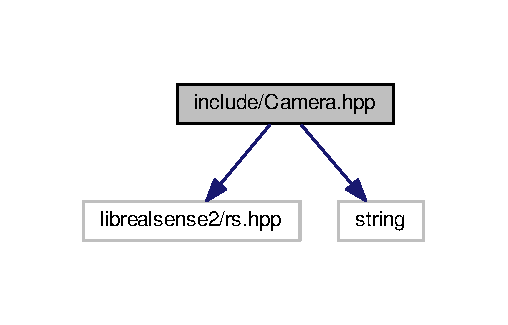
\includegraphics[width=244pt]{Camera_8hpp__incl}
\end{center}
\end{figure}
This graph shows which files directly or indirectly include this file\+:\nopagebreak
\begin{figure}[H]
\begin{center}
\leavevmode
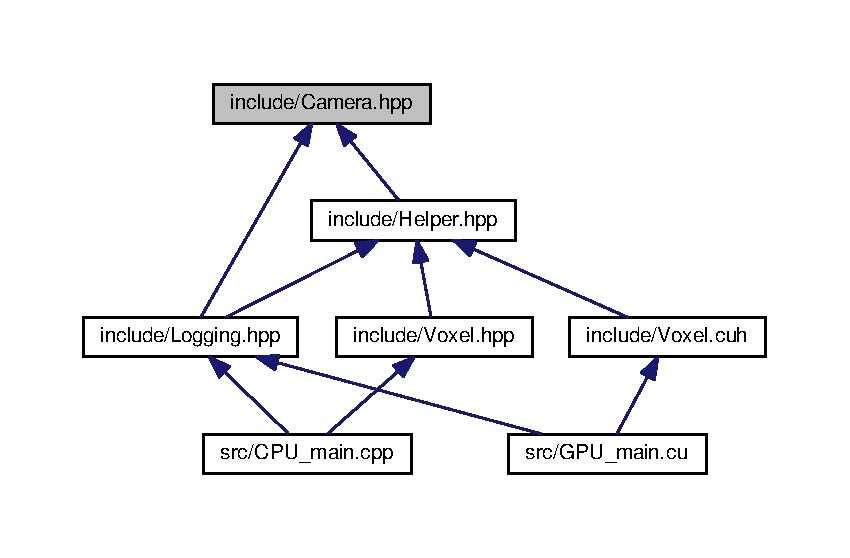
\includegraphics[width=350pt]{Camera_8hpp__dep__incl}
\end{center}
\end{figure}
\subsubsection*{Classes}
\begin{DoxyCompactItemize}
\item 
struct \hyperlink{structBool__Init}{Bool\+\_\+\+Init}
\begin{DoxyCompactList}\small\item\em Struct returned on \hyperlink{classCamera_a7f09b843d9b3a97e78eefcebbc53e054}{Camera\+::\+Init()} \end{DoxyCompactList}\item 
class \hyperlink{classCamera}{Camera}
\begin{DoxyCompactList}\small\item\em \hyperlink{classCamera}{Camera} streams abstraction class. \end{DoxyCompactList}\end{DoxyCompactItemize}
\subsubsection*{Macros}
\begin{DoxyCompactItemize}
\item 
\#define \hyperlink{Camera_8hpp_af7b7dc9a200cb1404c280bd500fd1551}{B\+U\+F\+F\+E\+R\+\_\+\+L\+E\+N\+G\+TH}~5
\begin{DoxyCompactList}\small\item\em Length of Queue Buffers for cameras. \end{DoxyCompactList}\item 
\#define \hyperlink{Camera_8hpp_a4a8be390afbe56038ccc6fe44e61aa00}{I\+N\+P\+U\+T\+\_\+\+R\+A\+TE}~50
\begin{DoxyCompactList}\small\item\em Maximum rate at which data receiving thread runs. \end{DoxyCompactList}\item 
\#define \hyperlink{Camera_8hpp_a9359f7c0a43a27865c6d2409e74645a6}{M\+A\+P\+\_\+\+U\+P\+D\+A\+T\+E\+\_\+\+R\+A\+TE}~10
\begin{DoxyCompactList}\small\item\em Rate at which the Global Map is updated. \end{DoxyCompactList}\end{DoxyCompactItemize}
\subsubsection*{Variables}
\begin{DoxyCompactItemize}
\item 
static const int \hyperlink{Camera_8hpp_ad56e71b7cc91ce32f920769b6eb31e03}{d\+\_\+fps} = 90
\begin{DoxyCompactList}\small\item\em Frame rate for D435. \end{DoxyCompactList}\end{DoxyCompactItemize}
\begin{Indent}{\bf D435\+: Image Dimensions}\par
\begin{DoxyCompactItemize}
\item 
static const int \hyperlink{Camera_8hpp_a66326676d44c838441a4dc39c85f599b}{w} = 640
\item 
static const int \hyperlink{Camera_8hpp_a3f40fea9b1040e381f08ddd4b026765d}{h} = 480
\begin{DoxyCompactList}\small\item\em Height. \end{DoxyCompactList}\end{DoxyCompactItemize}
\end{Indent}
{\bf }\par
\begin{DoxyCompactItemize}
\item 
static const double \hyperlink{Camera_8hpp_a8c14b0a57a757fa1eca7b19c2d0bd110}{D435\+\_\+\+M\+IN} = 0.\+11
\begin{DoxyCompactList}\small\item\em Minimum and maximum depth for D435. \end{DoxyCompactList}\item 
static const double \hyperlink{Camera_8hpp_a525f4d6ba7971b5fc8f0bc55ea826762}{D435\+\_\+\+M\+AX} = 2.\+00
\begin{DoxyCompactList}\small\item\em Minimum and maximum depth for D435. \end{DoxyCompactList}\end{DoxyCompactItemize}

\begin{Indent}{\bf Camera Serial Numbers}\par
\begin{DoxyCompactItemize}
\item 
static const std\+::string \hyperlink{Camera_8hpp_a08da237113fcf4a0fb79c89a2ba02bce}{D\+E\+P\+T\+H\+\_\+\+S\+NO} = \char`\"{}819612073628\char`\"{}
\begin{DoxyCompactList}\small\item\em Serial number of D435. \end{DoxyCompactList}\item 
static const std\+::string \hyperlink{Camera_8hpp_a97168636c8d72f641dc410554a42b2ec}{T\+R\+A\+C\+K\+\_\+\+S\+NO} = \char`\"{}905312110622\char`\"{}
\end{DoxyCompactItemize}
\end{Indent}


\subsubsection{Macro Definition Documentation}
\index{Camera.\+hpp@{Camera.\+hpp}!B\+U\+F\+F\+E\+R\+\_\+\+L\+E\+N\+G\+TH@{B\+U\+F\+F\+E\+R\+\_\+\+L\+E\+N\+G\+TH}}
\index{B\+U\+F\+F\+E\+R\+\_\+\+L\+E\+N\+G\+TH@{B\+U\+F\+F\+E\+R\+\_\+\+L\+E\+N\+G\+TH}!Camera.\+hpp@{Camera.\+hpp}}
\paragraph[{\texorpdfstring{B\+U\+F\+F\+E\+R\+\_\+\+L\+E\+N\+G\+TH}{BUFFER_LENGTH}}]{\setlength{\rightskip}{0pt plus 5cm}\#define B\+U\+F\+F\+E\+R\+\_\+\+L\+E\+N\+G\+TH~5}\hypertarget{Camera_8hpp_af7b7dc9a200cb1404c280bd500fd1551}{}\label{Camera_8hpp_af7b7dc9a200cb1404c280bd500fd1551}


Length of Queue Buffers for cameras. 



Definition at line \hyperlink{Camera_8hpp_source_l00038}{38} of file \hyperlink{Camera_8hpp_source}{Camera.\+hpp}.

\index{Camera.\+hpp@{Camera.\+hpp}!I\+N\+P\+U\+T\+\_\+\+R\+A\+TE@{I\+N\+P\+U\+T\+\_\+\+R\+A\+TE}}
\index{I\+N\+P\+U\+T\+\_\+\+R\+A\+TE@{I\+N\+P\+U\+T\+\_\+\+R\+A\+TE}!Camera.\+hpp@{Camera.\+hpp}}
\paragraph[{\texorpdfstring{I\+N\+P\+U\+T\+\_\+\+R\+A\+TE}{INPUT_RATE}}]{\setlength{\rightskip}{0pt plus 5cm}\#define I\+N\+P\+U\+T\+\_\+\+R\+A\+TE~50}\hypertarget{Camera_8hpp_a4a8be390afbe56038ccc6fe44e61aa00}{}\label{Camera_8hpp_a4a8be390afbe56038ccc6fe44e61aa00}


Maximum rate at which data receiving thread runs. 

\begin{DoxySeeAlso}{See also}
\hyperlink{CPU__main_8cpp}{C\+P\+U\+\_\+main.\+cpp}, G\+P\+U\+\_\+main.\+cpp 
\end{DoxySeeAlso}


Definition at line \hyperlink{Camera_8hpp_source_l00042}{42} of file \hyperlink{Camera_8hpp_source}{Camera.\+hpp}.

\index{Camera.\+hpp@{Camera.\+hpp}!M\+A\+P\+\_\+\+U\+P\+D\+A\+T\+E\+\_\+\+R\+A\+TE@{M\+A\+P\+\_\+\+U\+P\+D\+A\+T\+E\+\_\+\+R\+A\+TE}}
\index{M\+A\+P\+\_\+\+U\+P\+D\+A\+T\+E\+\_\+\+R\+A\+TE@{M\+A\+P\+\_\+\+U\+P\+D\+A\+T\+E\+\_\+\+R\+A\+TE}!Camera.\+hpp@{Camera.\+hpp}}
\paragraph[{\texorpdfstring{M\+A\+P\+\_\+\+U\+P\+D\+A\+T\+E\+\_\+\+R\+A\+TE}{MAP_UPDATE_RATE}}]{\setlength{\rightskip}{0pt plus 5cm}\#define M\+A\+P\+\_\+\+U\+P\+D\+A\+T\+E\+\_\+\+R\+A\+TE~10}\hypertarget{Camera_8hpp_a9359f7c0a43a27865c6d2409e74645a6}{}\label{Camera_8hpp_a9359f7c0a43a27865c6d2409e74645a6}


Rate at which the Global Map is updated. 

\begin{DoxySeeAlso}{See also}
\hyperlink{CPU__main_8cpp}{C\+P\+U\+\_\+main.\+cpp}, G\+P\+U\+\_\+main.\+cpp 
\end{DoxySeeAlso}


Definition at line \hyperlink{Camera_8hpp_source_l00046}{46} of file \hyperlink{Camera_8hpp_source}{Camera.\+hpp}.



\subsubsection{Variable Documentation}
\index{Camera.\+hpp@{Camera.\+hpp}!D435\+\_\+\+M\+AX@{D435\+\_\+\+M\+AX}}
\index{D435\+\_\+\+M\+AX@{D435\+\_\+\+M\+AX}!Camera.\+hpp@{Camera.\+hpp}}
\paragraph[{\texorpdfstring{D435\+\_\+\+M\+AX}{D435_MAX}}]{\setlength{\rightskip}{0pt plus 5cm}const double D435\+\_\+\+M\+AX = 2.\+00\hspace{0.3cm}{\ttfamily [static]}}\hypertarget{Camera_8hpp_a525f4d6ba7971b5fc8f0bc55ea826762}{}\label{Camera_8hpp_a525f4d6ba7971b5fc8f0bc55ea826762}


Minimum and maximum depth for D435. 

N\+O\+TE\+: don\textquotesingle{}t use D435\+\_\+\+M\+IN less than 0.\+11 m 

Definition at line \hyperlink{Camera_8hpp_source_l00027}{27} of file \hyperlink{Camera_8hpp_source}{Camera.\+hpp}.

\index{Camera.\+hpp@{Camera.\+hpp}!D435\+\_\+\+M\+IN@{D435\+\_\+\+M\+IN}}
\index{D435\+\_\+\+M\+IN@{D435\+\_\+\+M\+IN}!Camera.\+hpp@{Camera.\+hpp}}
\paragraph[{\texorpdfstring{D435\+\_\+\+M\+IN}{D435_MIN}}]{\setlength{\rightskip}{0pt plus 5cm}const double D435\+\_\+\+M\+IN = 0.\+11\hspace{0.3cm}{\ttfamily [static]}}\hypertarget{Camera_8hpp_a8c14b0a57a757fa1eca7b19c2d0bd110}{}\label{Camera_8hpp_a8c14b0a57a757fa1eca7b19c2d0bd110}


Minimum and maximum depth for D435. 

N\+O\+TE\+: don\textquotesingle{}t use D435\+\_\+\+M\+IN less than 0.\+11 m 

Definition at line \hyperlink{Camera_8hpp_source_l00026}{26} of file \hyperlink{Camera_8hpp_source}{Camera.\+hpp}.

\index{Camera.\+hpp@{Camera.\+hpp}!d\+\_\+fps@{d\+\_\+fps}}
\index{d\+\_\+fps@{d\+\_\+fps}!Camera.\+hpp@{Camera.\+hpp}}
\paragraph[{\texorpdfstring{d\+\_\+fps}{d_fps}}]{\setlength{\rightskip}{0pt plus 5cm}const int d\+\_\+fps = 90\hspace{0.3cm}{\ttfamily [static]}}\hypertarget{Camera_8hpp_ad56e71b7cc91ce32f920769b6eb31e03}{}\label{Camera_8hpp_ad56e71b7cc91ce32f920769b6eb31e03}


Frame rate for D435. 



Definition at line \hyperlink{Camera_8hpp_source_l00020}{20} of file \hyperlink{Camera_8hpp_source}{Camera.\+hpp}.

\index{Camera.\+hpp@{Camera.\+hpp}!D\+E\+P\+T\+H\+\_\+\+S\+NO@{D\+E\+P\+T\+H\+\_\+\+S\+NO}}
\index{D\+E\+P\+T\+H\+\_\+\+S\+NO@{D\+E\+P\+T\+H\+\_\+\+S\+NO}!Camera.\+hpp@{Camera.\+hpp}}
\paragraph[{\texorpdfstring{D\+E\+P\+T\+H\+\_\+\+S\+NO}{DEPTH_SNO}}]{\setlength{\rightskip}{0pt plus 5cm}const std\+::string D\+E\+P\+T\+H\+\_\+\+S\+NO = \char`\"{}819612073628\char`\"{}\hspace{0.3cm}{\ttfamily [static]}}\hypertarget{Camera_8hpp_a08da237113fcf4a0fb79c89a2ba02bce}{}\label{Camera_8hpp_a08da237113fcf4a0fb79c89a2ba02bce}


Serial number of D435. 



Definition at line \hyperlink{Camera_8hpp_source_l00033}{33} of file \hyperlink{Camera_8hpp_source}{Camera.\+hpp}.

\index{Camera.\+hpp@{Camera.\+hpp}!h@{h}}
\index{h@{h}!Camera.\+hpp@{Camera.\+hpp}}
\paragraph[{\texorpdfstring{h}{h}}]{\setlength{\rightskip}{0pt plus 5cm}const int h = 480\hspace{0.3cm}{\ttfamily [static]}}\hypertarget{Camera_8hpp_a3f40fea9b1040e381f08ddd4b026765d}{}\label{Camera_8hpp_a3f40fea9b1040e381f08ddd4b026765d}


Height. 



Definition at line \hyperlink{Camera_8hpp_source_l00017}{17} of file \hyperlink{Camera_8hpp_source}{Camera.\+hpp}.

\index{Camera.\+hpp@{Camera.\+hpp}!T\+R\+A\+C\+K\+\_\+\+S\+NO@{T\+R\+A\+C\+K\+\_\+\+S\+NO}}
\index{T\+R\+A\+C\+K\+\_\+\+S\+NO@{T\+R\+A\+C\+K\+\_\+\+S\+NO}!Camera.\+hpp@{Camera.\+hpp}}
\paragraph[{\texorpdfstring{T\+R\+A\+C\+K\+\_\+\+S\+NO}{TRACK_SNO}}]{\setlength{\rightskip}{0pt plus 5cm}const std\+::string T\+R\+A\+C\+K\+\_\+\+S\+NO = \char`\"{}905312110622\char`\"{}\hspace{0.3cm}{\ttfamily [static]}}\hypertarget{Camera_8hpp_a97168636c8d72f641dc410554a42b2ec}{}\label{Camera_8hpp_a97168636c8d72f641dc410554a42b2ec}
Serial number of T265 

Definition at line \hyperlink{Camera_8hpp_source_l00034}{34} of file \hyperlink{Camera_8hpp_source}{Camera.\+hpp}.

\index{Camera.\+hpp@{Camera.\+hpp}!w@{w}}
\index{w@{w}!Camera.\+hpp@{Camera.\+hpp}}
\paragraph[{\texorpdfstring{w}{w}}]{\setlength{\rightskip}{0pt plus 5cm}const int w = 640\hspace{0.3cm}{\ttfamily [static]}}\hypertarget{Camera_8hpp_a66326676d44c838441a4dc39c85f599b}{}\label{Camera_8hpp_a66326676d44c838441a4dc39c85f599b}
Width 

Definition at line \hyperlink{Camera_8hpp_source_l00015}{15} of file \hyperlink{Camera_8hpp_source}{Camera.\+hpp}.


\hypertarget{Camera_8hpp_source}{}\subsection{Camera.\+hpp}
\label{Camera_8hpp_source}\index{include/\+Camera.\+hpp@{include/\+Camera.\+hpp}}

\begin{DoxyCode}
00001 \textcolor{preprocessor}{#ifndef CAMERA\_H}
00002 \textcolor{preprocessor}{#define CAMERA\_H}
00003 
00004 
00005 \textcolor{preprocessor}{#include <librealsense2/rs.hpp>}     \textcolor{comment}{// Include RealSense Cross Platform API}
00006 
00007 \textcolor{preprocessor}{#include <string>}
00008 
00009 
00010 
00013 \textcolor{keyword}{static} \textcolor{keyword}{const} \textcolor{keywordtype}{int} \hyperlink{Camera_8hpp_a66326676d44c838441a4dc39c85f599b}{w} = 640;
\hypertarget{Camera_8hpp_source.tex_l00017}{}\hyperlink{Camera_8hpp_a3f40fea9b1040e381f08ddd4b026765d}{00017} \textcolor{keyword}{static} \textcolor{keyword}{const} \textcolor{keywordtype}{int} \hyperlink{Camera_8hpp_a3f40fea9b1040e381f08ddd4b026765d}{h} = 480;
00019 
\hypertarget{Camera_8hpp_source.tex_l00020}{}\hyperlink{Camera_8hpp_ad56e71b7cc91ce32f920769b6eb31e03}{00020} \textcolor{keyword}{static} \textcolor{keyword}{const} \textcolor{keywordtype}{int} \hyperlink{Camera_8hpp_ad56e71b7cc91ce32f920769b6eb31e03}{d\_fps} = 90; 
00021 
00023 
\hypertarget{Camera_8hpp_source.tex_l00026}{}\hyperlink{Camera_8hpp_a8c14b0a57a757fa1eca7b19c2d0bd110}{00026} \textcolor{keyword}{static} \textcolor{keyword}{const} \textcolor{keywordtype}{double} \hyperlink{Camera_8hpp_a8c14b0a57a757fa1eca7b19c2d0bd110}{D435\_MIN} = 0.11; \textcolor{comment}{// | - min and max depths of D435 (m)}
\hypertarget{Camera_8hpp_source.tex_l00027}{}\hyperlink{Camera_8hpp_a525f4d6ba7971b5fc8f0bc55ea826762}{00027} \textcolor{keyword}{static} \textcolor{keyword}{const} \textcolor{keywordtype}{double} \hyperlink{Camera_8hpp_a525f4d6ba7971b5fc8f0bc55ea826762}{D435\_MAX} = 2.00; \textcolor{comment}{// |}
00029 \textcolor{comment}{}
00032 \textcolor{keyword}{static} \textcolor{keyword}{const} std::string \hyperlink{Camera_8hpp_a08da237113fcf4a0fb79c89a2ba02bce}{DEPTH\_SNO} = \textcolor{stringliteral}{"819612073628"}; 
\hypertarget{Camera_8hpp_source.tex_l00034}{}\hyperlink{Camera_8hpp_a97168636c8d72f641dc410554a42b2ec}{00034} \textcolor{keyword}{static} \textcolor{keyword}{const} std::string \hyperlink{Camera_8hpp_a97168636c8d72f641dc410554a42b2ec}{TRACK\_SNO} = \textcolor{stringliteral}{"905312110622"}; 
00035 
\hypertarget{Camera_8hpp_source.tex_l00038}{}\hyperlink{Camera_8hpp_af7b7dc9a200cb1404c280bd500fd1551}{00038} \textcolor{preprocessor}{#define BUFFER\_LENGTH 5 // length of buffer for cameras}
00039 
\hypertarget{Camera_8hpp_source.tex_l00042}{}\hyperlink{Camera_8hpp_a4a8be390afbe56038ccc6fe44e61aa00}{00042} \textcolor{preprocessor}{#define INPUT\_RATE 50 // Rate at which camera feed is taken (Hz)       | - Maximum rates}
00043 
\hypertarget{Camera_8hpp_source.tex_l00046}{}\hyperlink{Camera_8hpp_a9359f7c0a43a27865c6d2409e74645a6}{00046} \textcolor{preprocessor}{#define MAP\_UPDATE\_RATE 10 // Rate at which global map is updated (Hz) |}
00047 
00048 
00049 
00050 
00052 
\hypertarget{Camera_8hpp_source.tex_l00055}{}\hyperlink{structBool__Init}{00055} \textcolor{keyword}{struct }\hyperlink{structBool__Init}{Bool\_Init} \{
\hypertarget{Camera_8hpp_source.tex_l00057}{}\hyperlink{structBool__Init_a28c7d578113b5a52c1706c10be8fe6c6}{00057}     \textcolor{keywordtype}{bool} \hyperlink{structBool__Init_a28c7d578113b5a52c1706c10be8fe6c6}{t265};
\hypertarget{Camera_8hpp_source.tex_l00059}{}\hyperlink{structBool__Init_a9b59846a335953ae88cad02cd9cf9b34}{00059}     \textcolor{keywordtype}{bool} \hyperlink{structBool__Init_a9b59846a335953ae88cad02cd9cf9b34}{d435};
00060 \};
00061 
00063 
\hypertarget{Camera_8hpp_source.tex_l00069}{}\hyperlink{classCamera}{00069} \textcolor{keyword}{class }\hyperlink{classCamera}{Camera} \{
00070 
00071 \textcolor{keyword}{private}:
00072 
00074 
\hypertarget{Camera_8hpp_source.tex_l00076}{}\hyperlink{classCamera_a4373bc8793e3bb1d6eb2cca3eb25a31e}{00076}     rs2::context \hyperlink{classCamera_a4373bc8793e3bb1d6eb2cca3eb25a31e}{ctx};
00077 
00078 \textcolor{keyword}{public}:
00079 
00081 
\hypertarget{Camera_8hpp_source.tex_l00085}{}\hyperlink{classCamera_a689d4141375d8f7fbf1651338c1ea9c0}{00085}     std::vector<rs2::pipeline> \hyperlink{classCamera_a689d4141375d8f7fbf1651338c1ea9c0}{pipelines}; \textcolor{comment}{// pipelines for depth and tracking cameras - 0:
       tracking, 1: depth}
00086 
00090     \textcolor{keywordtype}{float} scale; 
00092 
00093     \textcolor{keywordtype}{float} fx;
\hypertarget{Camera_8hpp_source.tex_l00096}{}\hyperlink{classCamera_a1472650e23f3df5f23dda7f94537e889}{00096}     \textcolor{keywordtype}{float} \hyperlink{classCamera_a1472650e23f3df5f23dda7f94537e889}{fy};
00098 
00099     \textcolor{keywordtype}{float} ppx;
\hypertarget{Camera_8hpp_source.tex_l00102}{}\hyperlink{classCamera_a0e51f157264b9c9e18feb584c5a6c606}{00102}     \textcolor{keywordtype}{float} \hyperlink{classCamera_a0e51f157264b9c9e18feb584c5a6c606}{ppy};
00104     \textcolor{keywordtype}{int} model;
\hypertarget{Camera_8hpp_source.tex_l00107}{}\hyperlink{classCamera_af6b42da84223170eb6434a3df1d677af}{00107}     \textcolor{keywordtype}{float} coeffs[5];
00109 
00113     rs2::frame\_queue d\_queue;
\hypertarget{Camera_8hpp_source.tex_l00117}{}\hyperlink{classCamera_ad8a4c52c0ae125ab8ca66902408f5e95}{00117}     rs2::frame\_queue \hyperlink{classCamera_ad8a4c52c0ae125ab8ca66902408f5e95}{t\_queue};
00119 
00121 
\hypertarget{Camera_8hpp_source.tex_l00124}{}\hyperlink{classCamera_a01f94c3543f56ede7af49dc778f19331}{00124}     \hyperlink{classCamera_a01f94c3543f56ede7af49dc778f19331}{Camera}(): d\_queue(\hyperlink{Camera_8hpp_af7b7dc9a200cb1404c280bd500fd1551}{BUFFER\_LENGTH}), t\_queue(\hyperlink{Camera_8hpp_af7b7dc9a200cb1404c280bd500fd1551}{BUFFER\_LENGTH}) \{\}
00125 
00127 
\hypertarget{Camera_8hpp_source.tex_l00135}{}\hyperlink{classCamera_a7f09b843d9b3a97e78eefcebbc53e054}{00135}     \hyperlink{structBool__Init}{Bool\_Init} \hyperlink{classCamera_a7f09b843d9b3a97e78eefcebbc53e054}{Init} () \textcolor{keyword}{try} \{
00136         \textcolor{keywordtype}{int} num\_dev = 0;
00137         std::vector<rs2::pipeline> temp;
00138         \textcolor{keywordtype}{int} d\_idx, t\_idx;
00139         \hyperlink{structBool__Init}{Bool\_Init} b \{\textcolor{keyword}{false}, \textcolor{keyword}{false}\};
00140 
00141         \textcolor{keywordflow}{for} (\textcolor{keyword}{auto}&& dev : ctx.query\_devices())
00142         \{
00143 
00144             rs2::pipeline pipe(ctx);
00145             rs2::config cfg;
00146             cfg.enable\_device(dev.get\_info(RS2\_CAMERA\_INFO\_SERIAL\_NUMBER));
00147             
00148             \textcolor{keywordflow}{if} (strcmp(dev.get\_info(RS2\_CAMERA\_INFO\_SERIAL\_NUMBER), &\hyperlink{Camera_8hpp_a08da237113fcf4a0fb79c89a2ba02bce}{DEPTH\_SNO}[0]) == 0) \{
00149                 cfg.enable\_stream(RS2\_STREAM\_DEPTH, \hyperlink{Camera_8hpp_a66326676d44c838441a4dc39c85f599b}{w}, \hyperlink{Camera_8hpp_a3f40fea9b1040e381f08ddd4b026765d}{h}, RS2\_FORMAT\_Z16, 
      \hyperlink{Camera_8hpp_ad56e71b7cc91ce32f920769b6eb31e03}{d\_fps});
00150                 std::cout << \textcolor{stringliteral}{"Depth Camera initialized: \{"} << \hyperlink{Camera_8hpp_a66326676d44c838441a4dc39c85f599b}{w} << \textcolor{stringliteral}{","} << \hyperlink{Camera_8hpp_a3f40fea9b1040e381f08ddd4b026765d}{h} << \textcolor{stringliteral}{"\}, 90 FPS\(\backslash\)n"};
00151 
00152                 rs2::pipeline\_profile profile = pipe.start(cfg);
00153                 \textcolor{keyword}{auto} stream = profile.get\_stream(RS2\_STREAM\_DEPTH).as<rs2::video\_stream\_profile>();
00154                 scale = profile.get\_device().first<rs2::depth\_sensor>().get\_depth\_scale();
00155                 \textcolor{keyword}{auto} intrinsics = stream.get\_intrinsics();
00156                 fx  = intrinsics.fx;
00157                 fy  = intrinsics.fy;
00158                 ppx = intrinsics.ppx;
00159                 ppy = intrinsics.ppy;
00160                 model = intrinsics.model;
00161                 \textcolor{keywordflow}{for} (\textcolor{keywordtype}{int} i = 0; i < 5; i++)
00162                     coeffs[i] = intrinsics.coeffs[i];
00163 
00164                 d\_idx = num\_dev;
00165                 b.d435 = \textcolor{keyword}{true};
00166             \}
00167             \textcolor{keywordflow}{else} \textcolor{keywordflow}{if} (strcmp(dev.get\_info(RS2\_CAMERA\_INFO\_SERIAL\_NUMBER), &
      \hyperlink{Camera_8hpp_a97168636c8d72f641dc410554a42b2ec}{TRACK\_SNO}[0]) == 0) \{
00168                 cfg.enable\_stream(RS2\_STREAM\_POSE, RS2\_FORMAT\_6DOF);
00169                 std::cout << \textcolor{stringliteral}{"Tracking Camera initialized: 6DoF\(\backslash\)n"};
00170 
00171                 pipe.start(cfg);
00172                 t\_idx = num\_dev;
00173                 b.t265 = \textcolor{keyword}{true};
00174             \}
00175             \textcolor{keywordflow}{else} \{
00176                 std::cout << \textcolor{stringliteral}{"Device not recognized. Serial Number: "} << dev.get\_info(
      RS2\_CAMERA\_INFO\_SERIAL\_NUMBER) << \textcolor{stringliteral}{"\(\backslash\)n"};
00177                 \textcolor{keywordflow}{return} b;
00178             \}
00179 
00180             temp.emplace\_back(pipe);
00181             num\_dev++;
00182         \}
00183 
00184         \textcolor{keywordflow}{if} (b.t265)
00185             pipelines.emplace\_back(temp[t\_idx]);
00186         \textcolor{keywordflow}{if} (b.d435)
00187             pipelines.emplace\_back(temp[d\_idx]);
00188 
00189         \textcolor{keywordflow}{return} b;
00190 
00191     \}
00192     \textcolor{keywordflow}{catch} (\textcolor{keyword}{const} rs2::error & e) \{
00193         std::cerr << \textcolor{stringliteral}{"RealSense error calling "} << e.get\_failed\_function() << \textcolor{stringliteral}{"("} << e.get\_failed\_args() <<
       \textcolor{stringliteral}{"):\(\backslash\)n    "} << e.what() << std::endl;
00194         \textcolor{keywordflow}{return} \hyperlink{structBool__Init}{Bool\_Init} \{\textcolor{keyword}{false}, \textcolor{keyword}{false}\};
00195     \}
00196     \textcolor{keywordflow}{catch} (\textcolor{keyword}{const} std::exception & e) \{
00197         std::cerr << e.what() << std::endl;
00198         \textcolor{keywordflow}{return} \hyperlink{structBool__Init}{Bool\_Init} \{\textcolor{keyword}{false}, \textcolor{keyword}{false}\};
00199     \}
00200 
00201 \};
00202 
00203 
00204 \textcolor{preprocessor}{#endif}
\end{DoxyCode}

\hypertarget{Helper_8hpp}{}\subsection{include/\+Helper.hpp File Reference}
\label{Helper_8hpp}\index{include/\+Helper.\+hpp@{include/\+Helper.\+hpp}}
{\ttfamily \#include \char`\"{}Camera.\+hpp\char`\"{}}\\*
{\ttfamily \#include $<$opencv2/opencv.\+hpp$>$}\\*
Include dependency graph for Helper.\+hpp\+:\nopagebreak
\begin{figure}[H]
\begin{center}
\leavevmode
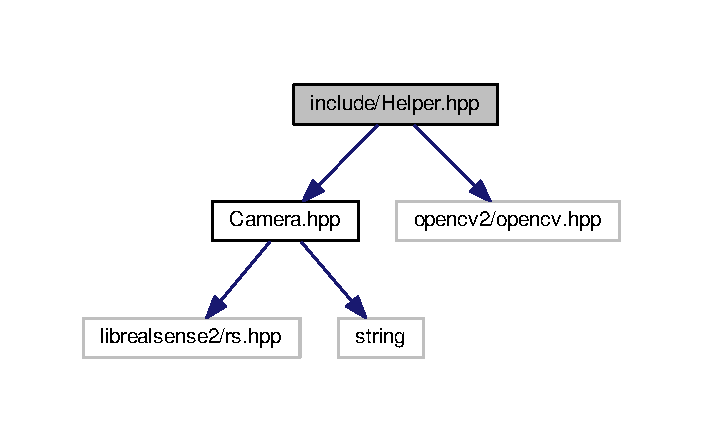
\includegraphics[width=338pt]{Helper_8hpp__incl}
\end{center}
\end{figure}
This graph shows which files directly or indirectly include this file\+:\nopagebreak
\begin{figure}[H]
\begin{center}
\leavevmode
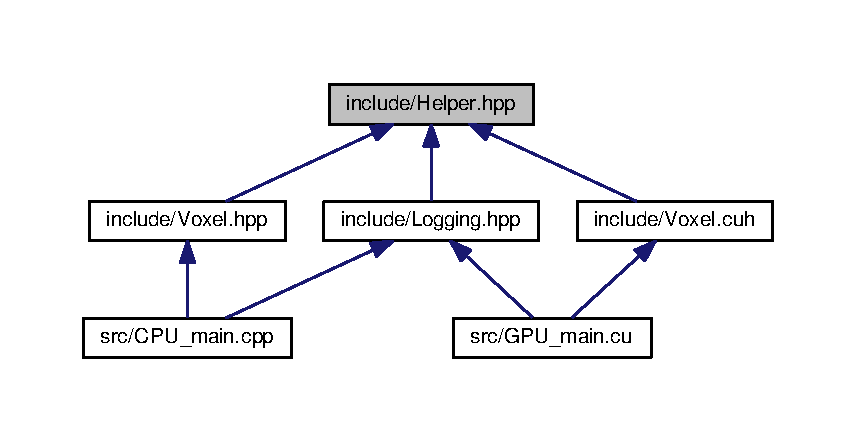
\includegraphics[width=350pt]{Helper_8hpp__dep__incl}
\end{center}
\end{figure}
\subsubsection*{Classes}
\begin{DoxyCompactItemize}
\item 
class \hyperlink{classPair}{Pair$<$ A, B $>$}
\begin{DoxyCompactList}\small\item\em Template Class for Pairs. \end{DoxyCompactList}\item 
class \hyperlink{classMap__FE}{Map\+\_\+\+FE}
\begin{DoxyCompactList}\small\item\em Virtual class Parent of \hyperlink{classCPU__FE}{C\+P\+U\+\_\+\+FE} and \hyperlink{classGPU__FE}{G\+P\+U\+\_\+\+FE} classes. \end{DoxyCompactList}\end{DoxyCompactItemize}
\subsubsection*{Macros}
\begin{DoxyCompactItemize}
\item 
\#define \hyperlink{Helper_8hpp_a0029886fd5e151820efb6eb46c000466}{C\+U\+D\+A\+\_\+\+C\+A\+LL}
\end{DoxyCompactItemize}


\subsubsection{Macro Definition Documentation}
\index{Helper.\+hpp@{Helper.\+hpp}!C\+U\+D\+A\+\_\+\+C\+A\+LL@{C\+U\+D\+A\+\_\+\+C\+A\+LL}}
\index{C\+U\+D\+A\+\_\+\+C\+A\+LL@{C\+U\+D\+A\+\_\+\+C\+A\+LL}!Helper.\+hpp@{Helper.\+hpp}}
\paragraph[{\texorpdfstring{C\+U\+D\+A\+\_\+\+C\+A\+LL}{CUDA_CALL}}]{\setlength{\rightskip}{0pt plus 5cm}\#define C\+U\+D\+A\+\_\+\+C\+A\+LL}\hypertarget{Helper_8hpp_a0029886fd5e151820efb6eb46c000466}{}\label{Helper_8hpp_a0029886fd5e151820efb6eb46c000466}


Definition at line \hyperlink{Helper_8hpp_source_l00007}{7} of file \hyperlink{Helper_8hpp_source}{Helper.\+hpp}.


\hypertarget{Helper_8hpp_source}{}\subsection{Helper.\+hpp}
\label{Helper_8hpp_source}\index{include/\+Helper.\+hpp@{include/\+Helper.\+hpp}}

\begin{DoxyCode}
00001 \textcolor{preprocessor}{#ifndef HELPER\_H}
00002 \textcolor{preprocessor}{#define HELPER\_H}
00003 
00004 \textcolor{preprocessor}{#ifdef \_\_CUDACC\_\_}
00005 \textcolor{preprocessor}{#define CUDA\_CALL \_\_host\_\_ \_\_device\_\_}
00006 \textcolor{preprocessor}{#else}
\hypertarget{Helper_8hpp_source.tex_l00007}{}\hyperlink{Helper_8hpp_a0029886fd5e151820efb6eb46c000466}{00007} \textcolor{preprocessor}{#define CUDA\_CALL}
00008 \textcolor{preprocessor}{#endif}
00009 
00010 
00011 \textcolor{preprocessor}{#include "\hyperlink{Camera_8hpp}{Camera.hpp}"}
00012 \textcolor{preprocessor}{#include <opencv2/opencv.hpp>}
00013 
00014 
00015 
00016 
00017 \textcolor{comment}{/* Use following template class as replacement for std::pair */}
00019 
00025 \textcolor{keyword}{template} <\textcolor{keyword}{typename} A, \textcolor{keyword}{typename} B>
\hypertarget{Helper_8hpp_source.tex_l00026}{}\hyperlink{classPair}{00026} \textcolor{keyword}{class }\hyperlink{classPair}{Pair} \{
00027 
00028 \textcolor{keyword}{public}:
00029 
\hypertarget{Helper_8hpp_source.tex_l00031}{}\hyperlink{classPair_a98924311a2986df358d3b1965f8abd06}{00031}     A \hyperlink{classPair_a98924311a2986df358d3b1965f8abd06}{first};
\hypertarget{Helper_8hpp_source.tex_l00033}{}\hyperlink{classPair_af49ec2d61a46cad5cd1227dba4932aff}{00033}     B \hyperlink{classPair_af49ec2d61a46cad5cd1227dba4932aff}{second};
00034 
00037 
00040     \hyperlink{Helper_8hpp_a0029886fd5e151820efb6eb46c000466}{CUDA\_CALL} \hyperlink{classPair_ab76fff1f93ef8974bec7430bd67b916d}{Pair} () = \textcolor{keywordflow}{default};
00041 
00043 
\hypertarget{Helper_8hpp_source.tex_l00046}{}\hyperlink{classPair_addd8fa451e9cc9e1ab0ee13ccb130966}{00046}     \hyperlink{Helper_8hpp_a0029886fd5e151820efb6eb46c000466}{CUDA\_CALL} \hyperlink{classPair_addd8fa451e9cc9e1ab0ee13ccb130966}{Pair} (\textcolor{keyword}{const} A a, \textcolor{keyword}{const} B b): first(a), second(b) \{ \}
00048 
00051     
00054 
\hypertarget{Helper_8hpp_source.tex_l00059}{}\hyperlink{classPair_ab2e5000f2ce579285f773fafca762fb7}{00059}     \hyperlink{Helper_8hpp_a0029886fd5e151820efb6eb46c000466}{CUDA\_CALL} \textcolor{keyword}{inline} \textcolor{keywordtype}{bool} operator < (Pair<A, B> \textcolor{keyword}{const} &P) \textcolor{keyword}{const} \{
00060         \textcolor{keywordflow}{return} (this->first < P.first);
00061     \}
00062 
\hypertarget{Helper_8hpp_source.tex_l00064}{}\hyperlink{classPair_a8e382aa87f8063084ecea74136a35ace}{00064}     \hyperlink{Helper_8hpp_a0029886fd5e151820efb6eb46c000466}{CUDA\_CALL} \textcolor{keyword}{inline} \textcolor{keywordtype}{bool} \hyperlink{classPair_a8e382aa87f8063084ecea74136a35ace}{operator == }(\hyperlink{classPair}{Pair<A, B>} \textcolor{keyword}{const} &P)\textcolor{keyword}{ const }\{
00065         \textcolor{keywordflow}{return} (this->first == P.\hyperlink{classPair_a98924311a2986df358d3b1965f8abd06}{first});
00066     \}
00068 
00069 \};
00070 
00071 
00073 
\hypertarget{Helper_8hpp_source.tex_l00082}{}\hyperlink{classMap__FE}{00082} \textcolor{keyword}{class }\hyperlink{classMap__FE}{Map\_FE} \{
00083 
00084 \textcolor{keyword}{public}:
00085 
00087 
00092     \textcolor{keyword}{virtual} \textcolor{keywordtype}{void} Update (\hyperlink{classCamera}{Camera} \textcolor{keyword}{const} &C, rs2\_pose \textcolor{keyword}{const} &pose, cv::Mat \textcolor{keyword}{const} &depth) = 0;
00093 
00095 
00100     \textcolor{keyword}{virtual} \textcolor{keywordtype}{void} Points (std::vector < std::tuple<float, float, float, float> > * points) = 0;
00101 
00102 \};
00103 
00104 
00105 \textcolor{preprocessor}{#endif}
\end{DoxyCode}

\hypertarget{Logging_8hpp}{}\subsection{include/\+Logging.hpp File Reference}
\label{Logging_8hpp}\index{include/\+Logging.\+hpp@{include/\+Logging.\+hpp}}
{\ttfamily \#include $<$opencv2/opencv.\+hpp$>$}\\*
{\ttfamily \#include $<$iostream$>$}\\*
{\ttfamily \#include $<$fstream$>$}\\*
{\ttfamily \#include $<$vector$>$}\\*
{\ttfamily \#include $<$unistd.\+h$>$}\\*
{\ttfamily \#include $<$chrono$>$}\\*
{\ttfamily \#include $<$time.\+h$>$}\\*
{\ttfamily \#include $<$string$>$}\\*
{\ttfamily \#include \char`\"{}gnuplot-\/iostream.\+h\char`\"{}}\\*
{\ttfamily \#include \char`\"{}Camera.\+hpp\char`\"{}}\\*
{\ttfamily \#include \char`\"{}Helper.\+hpp\char`\"{}}\\*
Include dependency graph for Logging.\+hpp\+:\nopagebreak
\begin{figure}[H]
\begin{center}
\leavevmode
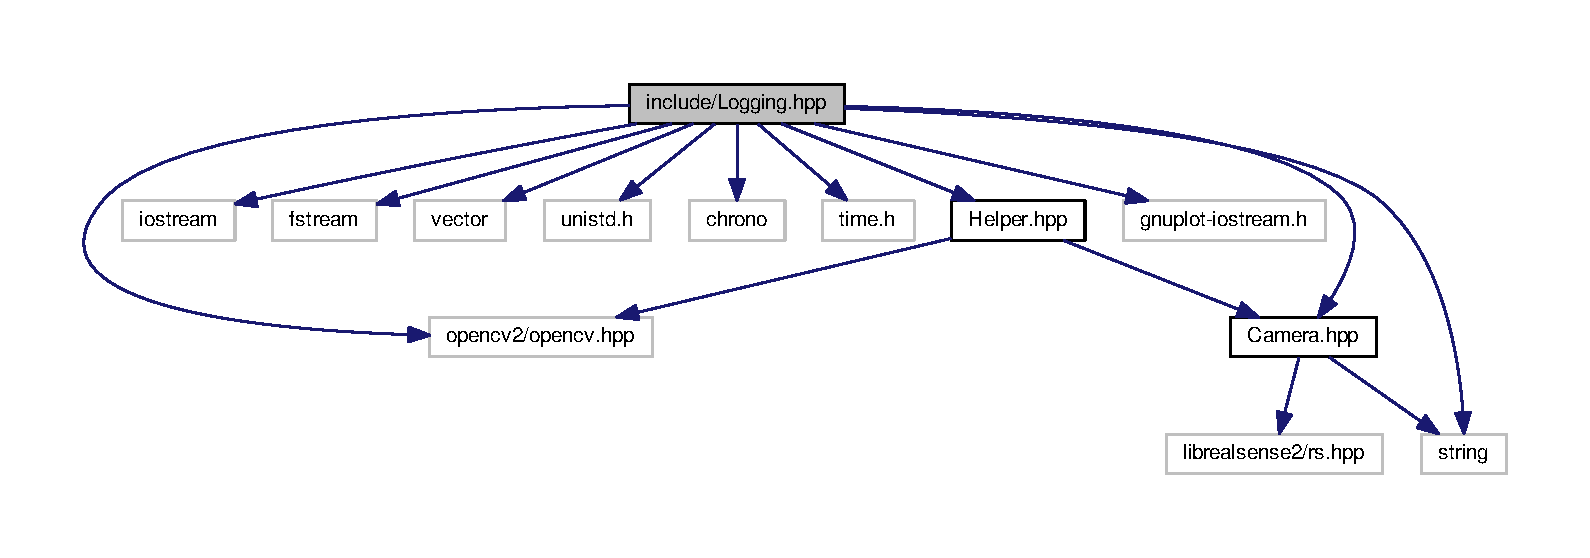
\includegraphics[width=350pt]{Logging_8hpp__incl}
\end{center}
\end{figure}
This graph shows which files directly or indirectly include this file\+:\nopagebreak
\begin{figure}[H]
\begin{center}
\leavevmode
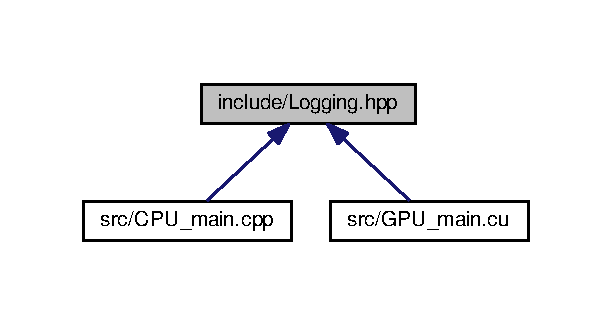
\includegraphics[width=294pt]{Logging_8hpp__dep__incl}
\end{center}
\end{figure}
\subsubsection*{Classes}
\begin{DoxyCompactItemize}
\item 
class \hyperlink{classLogger}{Logger}
\begin{DoxyCompactList}\small\item\em Logging class. \end{DoxyCompactList}\end{DoxyCompactItemize}
\subsubsection*{Variables}
\begin{DoxyCompactItemize}
\item 
static const std\+::string \hyperlink{Logging_8hpp_aa95bcbf818cd309e7d34d0309dc2932f}{L\+O\+G\+\_\+\+P\+A\+TH} = \char`\"{}/home/Akshay/Desktop/Test/Mapping/Logs/\char`\"{}
\begin{DoxyCompactList}\small\item\em The path where the log files will be stored. \end{DoxyCompactList}\end{DoxyCompactItemize}
{\bf }\par
\begin{DoxyCompactItemize}
\item 
static const bool \hyperlink{Logging_8hpp_a2fe143d334b5c5fd12da86fe05423074}{p\+\_\+logging} = true
\begin{DoxyCompactList}\small\item\em Logging constants. \end{DoxyCompactList}\item 
static const bool \hyperlink{Logging_8hpp_af862762a869dc8c1eda840a8ca645e15}{i\+\_\+logging} = true
\begin{DoxyCompactList}\small\item\em If set to true, depth intrinsics of D435 will be logged. \end{DoxyCompactList}\item 
static const bool \hyperlink{Logging_8hpp_adaf32a6a0736e8e3da49a3c2b0705fa7}{v\+\_\+logging} = false
\begin{DoxyCompactList}\small\item\em (Not recommended) If set to true, video feed from D435 will be logged. \end{DoxyCompactList}\item 
static const bool \hyperlink{Logging_8hpp_a3beae9ccc576e738591191c70cf26623}{m\+\_\+logging} = true
\begin{DoxyCompactList}\small\item\em If set to true, the global map is logged, which can be plotted using cmd \textquotesingle{}gnuplot Display.\+gp\textquotesingle{}. \end{DoxyCompactList}\item 
static const bool \hyperlink{Logging_8hpp_a5aa1661b54df291d66e2329c124e8f7b}{g\+\_\+logging} = false
\begin{DoxyCompactList}\small\item\em (Not recommended) If set to true, a grid visulaization of map is logged. \end{DoxyCompactList}\item 
static const bool \hyperlink{Logging_8hpp_aae489362ce8527e1feaba93222134df3}{display} = false
\begin{DoxyCompactList}\small\item\em (Turn off for performance) If set to true, the depth feed from D\$435 is displayed in real-\/time. \end{DoxyCompactList}\item 
static const bool \hyperlink{Logging_8hpp_a90bc243756c79ffb6d9c4a4ea99c41c2}{plot\+\_\+3d} = true
\begin{DoxyCompactList}\small\item\em (Turn off for performance) If set to true, a 3-\/D view of the depth feed from D435 is displayed. \end{DoxyCompactList}\end{DoxyCompactItemize}



\subsubsection{Variable Documentation}
\index{Logging.\+hpp@{Logging.\+hpp}!display@{display}}
\index{display@{display}!Logging.\+hpp@{Logging.\+hpp}}
\paragraph[{\texorpdfstring{display}{display}}]{\setlength{\rightskip}{0pt plus 5cm}const bool display = false\hspace{0.3cm}{\ttfamily [static]}}\hypertarget{Logging_8hpp_aae489362ce8527e1feaba93222134df3}{}\label{Logging_8hpp_aae489362ce8527e1feaba93222134df3}


(Turn off for performance) If set to true, the depth feed from D\$435 is displayed in real-\/time. 



Definition at line \hyperlink{Logging_8hpp_source_l00036}{36} of file \hyperlink{Logging_8hpp_source}{Logging.\+hpp}.

\index{Logging.\+hpp@{Logging.\+hpp}!g\+\_\+logging@{g\+\_\+logging}}
\index{g\+\_\+logging@{g\+\_\+logging}!Logging.\+hpp@{Logging.\+hpp}}
\paragraph[{\texorpdfstring{g\+\_\+logging}{g_logging}}]{\setlength{\rightskip}{0pt plus 5cm}const bool g\+\_\+logging = false\hspace{0.3cm}{\ttfamily [static]}}\hypertarget{Logging_8hpp_a5aa1661b54df291d66e2329c124e8f7b}{}\label{Logging_8hpp_a5aa1661b54df291d66e2329c124e8f7b}


(Not recommended) If set to true, a grid visulaization of map is logged. 



Definition at line \hyperlink{Logging_8hpp_source_l00034}{34} of file \hyperlink{Logging_8hpp_source}{Logging.\+hpp}.

\index{Logging.\+hpp@{Logging.\+hpp}!i\+\_\+logging@{i\+\_\+logging}}
\index{i\+\_\+logging@{i\+\_\+logging}!Logging.\+hpp@{Logging.\+hpp}}
\paragraph[{\texorpdfstring{i\+\_\+logging}{i_logging}}]{\setlength{\rightskip}{0pt plus 5cm}const bool i\+\_\+logging = true\hspace{0.3cm}{\ttfamily [static]}}\hypertarget{Logging_8hpp_af862762a869dc8c1eda840a8ca645e15}{}\label{Logging_8hpp_af862762a869dc8c1eda840a8ca645e15}


If set to true, depth intrinsics of D435 will be logged. 



Definition at line \hyperlink{Logging_8hpp_source_l00028}{28} of file \hyperlink{Logging_8hpp_source}{Logging.\+hpp}.

\index{Logging.\+hpp@{Logging.\+hpp}!L\+O\+G\+\_\+\+P\+A\+TH@{L\+O\+G\+\_\+\+P\+A\+TH}}
\index{L\+O\+G\+\_\+\+P\+A\+TH@{L\+O\+G\+\_\+\+P\+A\+TH}!Logging.\+hpp@{Logging.\+hpp}}
\paragraph[{\texorpdfstring{L\+O\+G\+\_\+\+P\+A\+TH}{LOG_PATH}}]{\setlength{\rightskip}{0pt plus 5cm}const std\+::string L\+O\+G\+\_\+\+P\+A\+TH = \char`\"{}/home/Akshay/Desktop/Test/Mapping/Logs/\char`\"{}\hspace{0.3cm}{\ttfamily [static]}}\hypertarget{Logging_8hpp_aa95bcbf818cd309e7d34d0309dc2932f}{}\label{Logging_8hpp_aa95bcbf818cd309e7d34d0309dc2932f}


The path where the log files will be stored. 



Definition at line \hyperlink{Logging_8hpp_source_l00042}{42} of file \hyperlink{Logging_8hpp_source}{Logging.\+hpp}.

\index{Logging.\+hpp@{Logging.\+hpp}!m\+\_\+logging@{m\+\_\+logging}}
\index{m\+\_\+logging@{m\+\_\+logging}!Logging.\+hpp@{Logging.\+hpp}}
\paragraph[{\texorpdfstring{m\+\_\+logging}{m_logging}}]{\setlength{\rightskip}{0pt plus 5cm}const bool m\+\_\+logging = true\hspace{0.3cm}{\ttfamily [static]}}\hypertarget{Logging_8hpp_a3beae9ccc576e738591191c70cf26623}{}\label{Logging_8hpp_a3beae9ccc576e738591191c70cf26623}


If set to true, the global map is logged, which can be plotted using cmd \textquotesingle{}gnuplot Display.\+gp\textquotesingle{}. 



Definition at line \hyperlink{Logging_8hpp_source_l00032}{32} of file \hyperlink{Logging_8hpp_source}{Logging.\+hpp}.

\index{Logging.\+hpp@{Logging.\+hpp}!p\+\_\+logging@{p\+\_\+logging}}
\index{p\+\_\+logging@{p\+\_\+logging}!Logging.\+hpp@{Logging.\+hpp}}
\paragraph[{\texorpdfstring{p\+\_\+logging}{p_logging}}]{\setlength{\rightskip}{0pt plus 5cm}const bool p\+\_\+logging = true\hspace{0.3cm}{\ttfamily [static]}}\hypertarget{Logging_8hpp_a2fe143d334b5c5fd12da86fe05423074}{}\label{Logging_8hpp_a2fe143d334b5c5fd12da86fe05423074}


Logging constants. 

The follwing boolean values determine the entities to be logged.\+If set to true, pose information from T265 will be logged. 

Definition at line \hyperlink{Logging_8hpp_source_l00026}{26} of file \hyperlink{Logging_8hpp_source}{Logging.\+hpp}.

\index{Logging.\+hpp@{Logging.\+hpp}!plot\+\_\+3d@{plot\+\_\+3d}}
\index{plot\+\_\+3d@{plot\+\_\+3d}!Logging.\+hpp@{Logging.\+hpp}}
\paragraph[{\texorpdfstring{plot\+\_\+3d}{plot_3d}}]{\setlength{\rightskip}{0pt plus 5cm}const bool plot\+\_\+3d = true\hspace{0.3cm}{\ttfamily [static]}}\hypertarget{Logging_8hpp_a90bc243756c79ffb6d9c4a4ea99c41c2}{}\label{Logging_8hpp_a90bc243756c79ffb6d9c4a4ea99c41c2}


(Turn off for performance) If set to true, a 3-\/D view of the depth feed from D435 is displayed. 



Definition at line \hyperlink{Logging_8hpp_source_l00038}{38} of file \hyperlink{Logging_8hpp_source}{Logging.\+hpp}.

\index{Logging.\+hpp@{Logging.\+hpp}!v\+\_\+logging@{v\+\_\+logging}}
\index{v\+\_\+logging@{v\+\_\+logging}!Logging.\+hpp@{Logging.\+hpp}}
\paragraph[{\texorpdfstring{v\+\_\+logging}{v_logging}}]{\setlength{\rightskip}{0pt plus 5cm}const bool v\+\_\+logging = false\hspace{0.3cm}{\ttfamily [static]}}\hypertarget{Logging_8hpp_adaf32a6a0736e8e3da49a3c2b0705fa7}{}\label{Logging_8hpp_adaf32a6a0736e8e3da49a3c2b0705fa7}


(Not recommended) If set to true, video feed from D435 will be logged. 



Definition at line \hyperlink{Logging_8hpp_source_l00030}{30} of file \hyperlink{Logging_8hpp_source}{Logging.\+hpp}.


\hypertarget{Logging_8hpp_source}{}\subsection{Logging.\+hpp}
\label{Logging_8hpp_source}\index{include/\+Logging.\+hpp@{include/\+Logging.\+hpp}}

\begin{DoxyCode}
00001 \textcolor{preprocessor}{#ifndef LOGGER\_H}
00002 \textcolor{preprocessor}{#define LOGGER\_H}
00003 
00004 
00005 \textcolor{preprocessor}{#include <opencv2/opencv.hpp>}
00006 
00007 \textcolor{preprocessor}{#include <iostream>}
00008 \textcolor{preprocessor}{#include <fstream>}
00009 \textcolor{preprocessor}{#include <vector>}
00010 \textcolor{preprocessor}{#include <unistd.h>}
00011 \textcolor{preprocessor}{#include <chrono>}
00012 \textcolor{preprocessor}{#include <time.h>}
00013 \textcolor{preprocessor}{#include <string>}
00014 
00015 \textcolor{preprocessor}{#include "gnuplot-iostream.h"}
00016 \textcolor{preprocessor}{#include "\hyperlink{Camera_8hpp}{Camera.hpp}"}
00017 \textcolor{preprocessor}{#include "\hyperlink{Helper_8hpp}{Helper.hpp}"}
00018 
00019 
00021 
00023 
\hypertarget{Logging_8hpp_source.tex_l00026}{}\hyperlink{Logging_8hpp_a2fe143d334b5c5fd12da86fe05423074}{00026} \textcolor{keyword}{static} \textcolor{keyword}{const} \textcolor{keywordtype}{bool} \hyperlink{Logging_8hpp_a2fe143d334b5c5fd12da86fe05423074}{p\_logging} = \textcolor{keyword}{true}; \textcolor{comment}{// logs pose data from T265}
\hypertarget{Logging_8hpp_source.tex_l00028}{}\hyperlink{Logging_8hpp_af862762a869dc8c1eda840a8ca645e15}{00028} \textcolor{comment}{}\textcolor{keyword}{static} \textcolor{keyword}{const} \textcolor{keywordtype}{bool} \hyperlink{Logging_8hpp_af862762a869dc8c1eda840a8ca645e15}{i\_logging} = \textcolor{keyword}{true}; \textcolor{comment}{// logs depth intrinsics data}
\hypertarget{Logging_8hpp_source.tex_l00030}{}\hyperlink{Logging_8hpp_adaf32a6a0736e8e3da49a3c2b0705fa7}{00030} \textcolor{comment}{}\textcolor{keyword}{static} \textcolor{keyword}{const} \textcolor{keywordtype}{bool} \hyperlink{Logging_8hpp_adaf32a6a0736e8e3da49a3c2b0705fa7}{v\_logging} = \textcolor{keyword}{false}; \textcolor{comment}{// logs depth feed from D435 (normalized) - use correct depth
       and video type}
\hypertarget{Logging_8hpp_source.tex_l00032}{}\hyperlink{Logging_8hpp_a3beae9ccc576e738591191c70cf26623}{00032} \textcolor{comment}{}\textcolor{keyword}{static} \textcolor{keyword}{const} \textcolor{keywordtype}{bool} \hyperlink{Logging_8hpp_a3beae9ccc576e738591191c70cf26623}{m\_logging} = \textcolor{keyword}{true}; \textcolor{comment}{// logs a point visualization for global map and trajectory}
\hypertarget{Logging_8hpp_source.tex_l00034}{}\hyperlink{Logging_8hpp_a5aa1661b54df291d66e2329c124e8f7b}{00034} \textcolor{comment}{}\textcolor{keyword}{static} \textcolor{keyword}{const} \textcolor{keywordtype}{bool} \hyperlink{Logging_8hpp_a5aa1661b54df291d66e2329c124e8f7b}{g\_logging} = \textcolor{keyword}{false}; \textcolor{comment}{// logs a grid visualization for global map - not recommended}
\hypertarget{Logging_8hpp_source.tex_l00036}{}\hyperlink{Logging_8hpp_aae489362ce8527e1feaba93222134df3}{00036} \textcolor{comment}{}\textcolor{keyword}{static} \textcolor{keyword}{const} \textcolor{keywordtype}{bool} \hyperlink{Logging_8hpp_aae489362ce8527e1feaba93222134df3}{display} = \textcolor{keyword}{false}; \textcolor{comment}{// displays depth feed (normalized)}
\hypertarget{Logging_8hpp_source.tex_l00038}{}\hyperlink{Logging_8hpp_a90bc243756c79ffb6d9c4a4ea99c41c2}{00038} \textcolor{comment}{}\textcolor{keyword}{static} \textcolor{keyword}{const} \textcolor{keywordtype}{bool} \hyperlink{Logging_8hpp_a90bc243756c79ffb6d9c4a4ea99c41c2}{plot\_3d} = \textcolor{keyword}{true}; \textcolor{comment}{// displays 3-D view of depth feed from D435}
00040 \textcolor{comment}{}
\hypertarget{Logging_8hpp_source.tex_l00042}{}\hyperlink{Logging_8hpp_aa95bcbf818cd309e7d34d0309dc2932f}{00042} \textcolor{keyword}{static} \textcolor{keyword}{const} std::string \hyperlink{Logging_8hpp_aa95bcbf818cd309e7d34d0309dc2932f}{LOG\_PATH} = \textcolor{stringliteral}{"/home/Akshay/Desktop/Test/Mapping/Logs/"}; \textcolor{comment}{// path for logging}
00043 
00044 
00045 
00047 
\hypertarget{Logging_8hpp_source.tex_l00052}{}\hyperlink{classLogger}{00052} \textcolor{keyword}{class }\hyperlink{classLogger}{Logger} \{
00053 
00054 \textcolor{keyword}{private}:
00055 
\hypertarget{Logging_8hpp_source.tex_l00057}{}\hyperlink{classLogger_a99c616f02a46e95f2e976ab7d880dbc5}{00057}     \textcolor{keywordtype}{bool} \hyperlink{classLogger_a99c616f02a46e95f2e976ab7d880dbc5}{start};
00058 
\hypertarget{Logging_8hpp_source.tex_l00060}{}\hyperlink{classLogger_a7f6f65922677036ca61ba12a19fdb719}{00060}     std::chrono::high\_resolution\_clock::time\_point \hyperlink{classLogger_a7f6f65922677036ca61ba12a19fdb719}{ti};
00061 
\hypertarget{Logging_8hpp_source.tex_l00063}{}\hyperlink{classLogger_afe5c4b612d69878aa65ce940a042fd8c}{00063}     time\_t \hyperlink{classLogger_afe5c4b612d69878aa65ce940a042fd8c}{today};
\hypertarget{Logging_8hpp_source.tex_l00065}{}\hyperlink{classLogger_a0fd4efa39e08c0253f59f76e08abefee}{00065}     \textcolor{keywordtype}{char} \hyperlink{classLogger_a0fd4efa39e08c0253f59f76e08abefee}{buf}[80];
00066     
00067     \textcolor{comment}{/* output files for logging */}
00070 
\hypertarget{Logging_8hpp_source.tex_l00072}{}\hyperlink{classLogger_a7314c685ce4579a7d8b118e5d5327d13}{00072}     std::ofstream \hyperlink{classLogger_a7314c685ce4579a7d8b118e5d5327d13}{pose\_file};
\hypertarget{Logging_8hpp_source.tex_l00074}{}\hyperlink{classLogger_acf9b6a89a6f8c520d010d87cff33b9df}{00074}     std::ofstream \hyperlink{classLogger_acf9b6a89a6f8c520d010d87cff33b9df}{d\_in\_file};
\hypertarget{Logging_8hpp_source.tex_l00076}{}\hyperlink{classLogger_a5e5b9ad704575bda69b184a5b136735f}{00076}     cv::VideoWriter \hyperlink{classLogger_a5e5b9ad704575bda69b184a5b136735f}{depth\_file};
\hypertarget{Logging_8hpp_source.tex_l00078}{}\hyperlink{classLogger_a1aedce7141d1346bc39c94e3a3eba4d6}{00078}     std::ofstream \hyperlink{classLogger_a1aedce7141d1346bc39c94e3a3eba4d6}{map\_file};
\hypertarget{Logging_8hpp_source.tex_l00080}{}\hyperlink{classLogger_a715ae637741f3b00ba8ebb9858cb5577}{00080}     std::ofstream \hyperlink{classLogger_a715ae637741f3b00ba8ebb9858cb5577}{grid\_file};
00082 
\hypertarget{Logging_8hpp_source.tex_l00084}{}\hyperlink{classLogger_a63eca256c57dee44717f3002654887c7}{00084}     Gnuplot \hyperlink{classLogger_a63eca256c57dee44717f3002654887c7}{gp};
00085 
00086 \textcolor{keyword}{public}:
00087 
00089 
\hypertarget{Logging_8hpp_source.tex_l00091}{}\hyperlink{classLogger_abc41bfb031d896170c7675fa96a6b30c}{00091}     \hyperlink{classLogger_abc41bfb031d896170c7675fa96a6b30c}{Logger} () \{
00092         today = time(0);
00093         strftime (buf, \textcolor{keyword}{sizeof}(buf), \textcolor{stringliteral}{"%Y\_%m\_%d\_%H\_%M\_%S"}, localtime(&today));
00094         start = \textcolor{keyword}{false};
00095     \}
00096 
00098 
\hypertarget{Logging_8hpp_source.tex_l00100}{}\hyperlink{classLogger_a42c282f4c0e2c6557d16e2967c1ddf7e}{00100}     \textcolor{keywordtype}{void} \hyperlink{classLogger_a42c282f4c0e2c6557d16e2967c1ddf7e}{Init}() \{
00101         \textcolor{keywordflow}{if} (\hyperlink{Logging_8hpp_a2fe143d334b5c5fd12da86fe05423074}{p\_logging})
00102             pose\_file.open(\hyperlink{Logging_8hpp_aa95bcbf818cd309e7d34d0309dc2932f}{LOG\_PATH}+\textcolor{stringliteral}{"pose.tsv"});
00103         \textcolor{keywordflow}{if} (\hyperlink{Logging_8hpp_af862762a869dc8c1eda840a8ca645e15}{i\_logging})
00104             d\_in\_file.open(\hyperlink{Logging_8hpp_aa95bcbf818cd309e7d34d0309dc2932f}{LOG\_PATH}+\textcolor{stringliteral}{"intrinsics.csv"});
00105         \textcolor{keywordflow}{if} (\hyperlink{Logging_8hpp_adaf32a6a0736e8e3da49a3c2b0705fa7}{v\_logging})
00106             depth\_file.open(\hyperlink{Logging_8hpp_aa95bcbf818cd309e7d34d0309dc2932f}{LOG\_PATH}+std::string(buf)+\textcolor{stringliteral}{".avi"}, CV\_FOURCC(\textcolor{charliteral}{'F'},\textcolor{charliteral}{'F'},\textcolor{charliteral}{'V'},\textcolor{charliteral}{'1'}), 
      \hyperlink{Camera_8hpp_a4a8be390afbe56038ccc6fe44e61aa00}{INPUT\_RATE}, cv::Size(\hyperlink{Camera_8hpp_a66326676d44c838441a4dc39c85f599b}{w},\hyperlink{Camera_8hpp_a3f40fea9b1040e381f08ddd4b026765d}{h}), \textcolor{keyword}{false});
00107         \textcolor{keywordflow}{if} (\hyperlink{Logging_8hpp_a3beae9ccc576e738591191c70cf26623}{m\_logging})
00108             map\_file.open(\hyperlink{Logging_8hpp_aa95bcbf818cd309e7d34d0309dc2932f}{LOG\_PATH}+\textcolor{stringliteral}{"map.tsv"});
00109         \textcolor{keywordflow}{if} (\hyperlink{Logging_8hpp_a5aa1661b54df291d66e2329c124e8f7b}{g\_logging})
00110             grid\_file.open(\hyperlink{Logging_8hpp_aa95bcbf818cd309e7d34d0309dc2932f}{LOG\_PATH}+\textcolor{stringliteral}{"grid.gp"});
00111     \}
00112 
00114 
\hypertarget{Logging_8hpp_source.tex_l00121}{}\hyperlink{classLogger_adcc95257ff2edceded8e272dac3603ce}{00121}     \textcolor{keywordtype}{void} \hyperlink{classLogger_adcc95257ff2edceded8e272dac3603ce}{Log} (\hyperlink{classCamera}{Camera} \textcolor{keyword}{const} * C, rs2\_pose \textcolor{keyword}{const} * pose, cv::Mat \textcolor{keyword}{const} * depth) \{
00122         \textcolor{keywordtype}{float} xl, yu, xr, yd;
00123         xl = -C->\hyperlink{classCamera_aa646a2de04e9ad37395dcf3c4a171abe}{ppx}/C->\hyperlink{classCamera_a4f5e789525c1c9306028c080922582e2}{fx}*\hyperlink{Camera_8hpp_a525f4d6ba7971b5fc8f0bc55ea826762}{D435\_MAX}; xr = (\hyperlink{Camera_8hpp_a66326676d44c838441a4dc39c85f599b}{w}-1-C->\hyperlink{classCamera_aa646a2de04e9ad37395dcf3c4a171abe}{ppx})/C->\hyperlink{classCamera_a4f5e789525c1c9306028c080922582e2}{fx}*
      \hyperlink{Camera_8hpp_a525f4d6ba7971b5fc8f0bc55ea826762}{D435\_MAX};
00124         yu = -C->\hyperlink{classCamera_a0e51f157264b9c9e18feb584c5a6c606}{ppy}/C->\hyperlink{classCamera_a1472650e23f3df5f23dda7f94537e889}{fy}*\hyperlink{Camera_8hpp_a525f4d6ba7971b5fc8f0bc55ea826762}{D435\_MAX}; yd = (\hyperlink{Camera_8hpp_a3f40fea9b1040e381f08ddd4b026765d}{h}-1-C->\hyperlink{classCamera_a0e51f157264b9c9e18feb584c5a6c606}{ppy})/C->\hyperlink{classCamera_a1472650e23f3df5f23dda7f94537e889}{fy}*
      \hyperlink{Camera_8hpp_a525f4d6ba7971b5fc8f0bc55ea826762}{D435\_MAX};
00125 
00126         \textcolor{keywordflow}{if} (!start) \{
00127             ti = std::chrono::high\_resolution\_clock::now();
00128             start = \textcolor{keyword}{true};
00129             \textcolor{keywordflow}{if} (\hyperlink{Logging_8hpp_a90bc243756c79ffb6d9c4a4ea99c41c2}{plot\_3d}) \{
00130                 gp << \textcolor{stringliteral}{"set view 180, 0\(\backslash\)n"};
00131                 gp << \textcolor{stringliteral}{"set xrange ["}<<xl<<\textcolor{stringliteral}{":"}<<xr<<\textcolor{stringliteral}{"]\(\backslash\)n"};
00132                 gp << \textcolor{stringliteral}{"set yrange ["}<<yu<<\textcolor{stringliteral}{":"}<<yd<<\textcolor{stringliteral}{"]\(\backslash\)n"};
00133                 gp << \textcolor{stringliteral}{"set zrange [0:"}<<\hyperlink{Camera_8hpp_a525f4d6ba7971b5fc8f0bc55ea826762}{D435\_MAX}<<\textcolor{stringliteral}{"]\(\backslash\)n"};
00134                 gp << \textcolor{stringliteral}{"set cbrange [0:"}<<D435\_MAX<<\textcolor{stringliteral}{"]\(\backslash\)n"};
00135             \}
00136         \}
00137 
00138         \textcolor{keyword}{auto} tf = std::chrono::high\_resolution\_clock::now() - \hyperlink{classLogger_a7f6f65922677036ca61ba12a19fdb719}{ti};
00139         \textcolor{keywordtype}{double} t = std::chrono::duration\_cast<std::chrono::milliseconds>(tf).count();
00140         \textcolor{keywordflow}{if} (\hyperlink{Logging_8hpp_adaf32a6a0736e8e3da49a3c2b0705fa7}{v\_logging} || \hyperlink{Logging_8hpp_aae489362ce8527e1feaba93222134df3}{display}) \{
00141             cv::Mat adj\_depth;
00142             cv::convertScaleAbs(*depth, adj\_depth, 255.0/65535.0);
00143             cv::threshold (adj\_depth, adj\_depth, \hyperlink{Camera_8hpp_a525f4d6ba7971b5fc8f0bc55ea826762}{D435\_MAX}/C->\hyperlink{classCamera_a50152f7c8f2ce7601dd6086c90b3a65c}{scale} * 255.0/65535.0, 0, 
      cv::THRESH\_TRUNC);
00144             cv::convertScaleAbs(adj\_depth, adj\_depth, 65535.0*C->\hyperlink{classCamera_a50152f7c8f2ce7601dd6086c90b3a65c}{scale}/
      \hyperlink{Camera_8hpp_a525f4d6ba7971b5fc8f0bc55ea826762}{D435\_MAX});
00145 
00146             \textcolor{keywordflow}{if} (\hyperlink{Logging_8hpp_adaf32a6a0736e8e3da49a3c2b0705fa7}{v\_logging})
00147                 depth\_file.write(adj\_depth);
00148 
00149             \textcolor{keywordflow}{if} (\hyperlink{Logging_8hpp_aae489362ce8527e1feaba93222134df3}{display})
00150                 imshow (\textcolor{stringliteral}{"Depth Image"}, adj\_depth);
00151         \}
00152         \textcolor{keywordflow}{if} (\hyperlink{Logging_8hpp_a2fe143d334b5c5fd12da86fe05423074}{p\_logging})
00153             pose\_file << t << \textcolor{stringliteral}{" "} << pose->translation.x << \textcolor{stringliteral}{" "} << pose->translation.y << \textcolor{stringliteral}{" "} << pose->
      translation.z << \textcolor{stringliteral}{" "} << pose->rotation.w << \textcolor{stringliteral}{" "} << pose->rotation.x << \textcolor{stringliteral}{" "} << pose->rotation.y << \textcolor{stringliteral}{" "} << pose->
      rotation.z << \textcolor{stringliteral}{" "} << pose->tracker\_confidence << \textcolor{stringliteral}{"\(\backslash\)n"};
00154 
00155         \textcolor{keywordflow}{if} (\hyperlink{Logging_8hpp_a90bc243756c79ffb6d9c4a4ea99c41c2}{plot\_3d}) \{
00156             \textcolor{keywordtype}{float} x\_D435, y\_D435, z\_D435;
00157             std::vector< std::tuple<float, float, float> > points;
00158             points.push\_back(std::make\_tuple(0, 0, 0));
00159             \textcolor{keywordflow}{for} (\textcolor{keywordtype}{int} i = 0; i < \hyperlink{Camera_8hpp_a3f40fea9b1040e381f08ddd4b026765d}{h}; i+=10) \{
00160                 \textcolor{keywordflow}{for} (\textcolor{keywordtype}{int} j = 0; j < \hyperlink{Camera_8hpp_a66326676d44c838441a4dc39c85f599b}{w}; j+=10) \{
00161                     z\_D435 = depth->at<\textcolor{keywordtype}{unsigned} \textcolor{keywordtype}{short} \textcolor{keywordtype}{int}>(i,j) * C->\hyperlink{classCamera_a50152f7c8f2ce7601dd6086c90b3a65c}{scale};
00162                     x\_D435 = (j-C->\hyperlink{classCamera_aa646a2de04e9ad37395dcf3c4a171abe}{ppx})/C->\hyperlink{classCamera_a4f5e789525c1c9306028c080922582e2}{fx} * z\_D435;
00163                     y\_D435 = (i-C->\hyperlink{classCamera_a0e51f157264b9c9e18feb584c5a6c606}{ppy})/C->\hyperlink{classCamera_a1472650e23f3df5f23dda7f94537e889}{fy} * z\_D435;
00164 
00165                     if (z\_D435 >= \hyperlink{Camera_8hpp_a8c14b0a57a757fa1eca7b19c2d0bd110}{D435\_MIN} && z\_D435 <= \hyperlink{Camera_8hpp_a525f4d6ba7971b5fc8f0bc55ea826762}{D435\_MAX})
00166                         points.push\_back(std::make\_tuple(x\_D435, y\_D435, z\_D435));
00167                 \}
00168             \}
00169             gp << \textcolor{stringliteral}{"set key off\(\backslash\)n"};
00170             gp << \textcolor{stringliteral}{"set view equal xyz\(\backslash\)n"};
00171             gp << \textcolor{stringliteral}{"set object polygon from "}<<xl<<\textcolor{stringliteral}{","}<<yu<<\textcolor{stringliteral}{","}<<\hyperlink{Camera_8hpp_a525f4d6ba7971b5fc8f0bc55ea826762}{D435\_MAX}<<\textcolor{stringliteral}{" to "}<<xr<<\textcolor{stringliteral}{","}<<yu<<\textcolor{stringliteral}{","}<
      <\hyperlink{Camera_8hpp_a525f4d6ba7971b5fc8f0bc55ea826762}{D435\_MAX}<<\textcolor{stringliteral}{" to "}<<xr<<\textcolor{stringliteral}{","}<<yd<<\textcolor{stringliteral}{","}<<\hyperlink{Camera_8hpp_a525f4d6ba7971b5fc8f0bc55ea826762}{D435\_MAX}<<\textcolor{stringliteral}{" to "}<<xl<<\textcolor{stringliteral}{","}<<yd<<\textcolor{stringliteral}{","}<<
      \hyperlink{Camera_8hpp_a525f4d6ba7971b5fc8f0bc55ea826762}{D435\_MAX}<<\textcolor{stringliteral}{" to "}<<xl<<\textcolor{stringliteral}{","}<<yu<<\textcolor{stringliteral}{","}<<\hyperlink{Camera_8hpp_a525f4d6ba7971b5fc8f0bc55ea826762}{D435\_MAX}<<\textcolor{stringliteral}{" fs transparent solid 0 fc rgb 'black' lw
       0.1\(\backslash\)n"};
00172             gp << \textcolor{stringliteral}{"splot '-' using 1:2:3 with points pointsize 0.25 pointtype 8 palette, \(\backslash\)\(\backslash\)\(\backslash\)n"};
00173             gp << \textcolor{stringliteral}{"'-' using 1:2:3:($4-$1):($5-$2):($6-$3) with vectors nohead lc rgb 'black' lw 0.25\(\backslash\)n"};
00174             gp.send1d(points);
00175             gp << \textcolor{stringliteral}{"0 0 0 "}<<xl<<\textcolor{stringliteral}{" "}<<yu<<\textcolor{stringliteral}{" "}<<D435\_MAX<<\textcolor{stringliteral}{"\(\backslash\)n"};
00176             gp << \textcolor{stringliteral}{"0 0 0 "}<<xr<<\textcolor{stringliteral}{" "}<<yu<<\textcolor{stringliteral}{" "}<<D435\_MAX<<\textcolor{stringliteral}{"\(\backslash\)n"};
00177             gp << \textcolor{stringliteral}{"0 0 0 "}<<xr<<\textcolor{stringliteral}{" "}<<yd<<\textcolor{stringliteral}{" "}<<D435\_MAX<<\textcolor{stringliteral}{"\(\backslash\)n"};
00178             gp << \textcolor{stringliteral}{"0 0 0 "}<<xl<<\textcolor{stringliteral}{" "}<<yd<<\textcolor{stringliteral}{" "}<<D435\_MAX<<\textcolor{stringliteral}{"\(\backslash\)n"};
00179             gp << \textcolor{stringliteral}{"e\(\backslash\)n"};
00180             gp << \textcolor{stringliteral}{"pause 0.05\(\backslash\)n"};
00181         \}
00182 
00183     \}
00184 
00186 
\hypertarget{Logging_8hpp_source.tex_l00192}{}\hyperlink{classLogger_a6b670ceb54a249eb83da08a1914d2be8}{00192}     \textcolor{keywordtype}{void} \hyperlink{classLogger_a6b670ceb54a249eb83da08a1914d2be8}{Close}(\hyperlink{classCamera}{Camera} \textcolor{keyword}{const} * C, \hyperlink{classMap__FE}{Map\_FE} * F) \{
00193         \textcolor{keywordflow}{if} (\hyperlink{Logging_8hpp_adaf32a6a0736e8e3da49a3c2b0705fa7}{v\_logging})
00194             depth\_file.release();
00195         \textcolor{keywordflow}{if} (\hyperlink{Logging_8hpp_a3beae9ccc576e738591191c70cf26623}{m\_logging}) \{
00196             std::vector< std::tuple<float, float, float, float> > points;
00197             F->\hyperlink{classMap__FE_aedfee41631a7287c9eb377ccb05317d6}{Points}(&points);
00198             \textcolor{keywordflow}{for} (std::vector< std::tuple<float, float, float, float> >::iterator it = points.begin(); it !=
       points.end(); it++) \{
00199                 map\_file << std::get<0>(*it) << \textcolor{stringliteral}{" "} << std::get<1>(*it) << \textcolor{stringliteral}{" "} << std::get<2>(*it) << \textcolor{stringliteral}{" "} <
      < std::get<3>(*it) << \textcolor{stringliteral}{"\(\backslash\)n"};
00200             \}
00201             map\_file.close();
00202         \}
00203         \textcolor{keywordflow}{if} (\hyperlink{Logging_8hpp_a2fe143d334b5c5fd12da86fe05423074}{p\_logging})
00204             pose\_file.close();
00205         \textcolor{keywordflow}{if} (\hyperlink{Logging_8hpp_af862762a869dc8c1eda840a8ca645e15}{i\_logging}) \{
00206             d\_in\_file << \textcolor{stringliteral}{"scale,"} << C->\hyperlink{classCamera_a50152f7c8f2ce7601dd6086c90b3a65c}{scale} << \textcolor{stringliteral}{"\(\backslash\)n"};
00207             d\_in\_file << \textcolor{stringliteral}{"focal length,"} << C->\hyperlink{classCamera_a4f5e789525c1c9306028c080922582e2}{fx} << \textcolor{stringliteral}{","} << C->\hyperlink{classCamera_a1472650e23f3df5f23dda7f94537e889}{fy} << \textcolor{stringliteral}{"\(\backslash\)n"};
00208             d\_in\_file << \textcolor{stringliteral}{"center,"} << C->\hyperlink{classCamera_aa646a2de04e9ad37395dcf3c4a171abe}{ppx} << \textcolor{stringliteral}{","} << C->\hyperlink{classCamera_a0e51f157264b9c9e18feb584c5a6c606}{ppy} << \textcolor{stringliteral}{"\(\backslash\)n"};
00209             d\_in\_file << \textcolor{stringliteral}{"distortion model,"} << C->\hyperlink{classCamera_a3061c56d262cab256468f05b9d8838fc}{model} << \textcolor{stringliteral}{"\(\backslash\)n"};
00210             d\_in\_file << \textcolor{stringliteral}{"coefficients,"} << C->\hyperlink{classCamera_af6b42da84223170eb6434a3df1d677af}{coeffs}[0] << \textcolor{stringliteral}{","} << C->
      \hyperlink{classCamera_af6b42da84223170eb6434a3df1d677af}{coeffs}[1] << \textcolor{stringliteral}{","} << C->\hyperlink{classCamera_af6b42da84223170eb6434a3df1d677af}{coeffs}[2] << \textcolor{stringliteral}{","} << C->\hyperlink{classCamera_af6b42da84223170eb6434a3df1d677af}{coeffs}[3] << \textcolor{stringliteral}{","} << C->
      \hyperlink{classCamera_af6b42da84223170eb6434a3df1d677af}{coeffs}[4] << \textcolor{stringliteral}{"\(\backslash\)n"};
00211             d\_in\_file.close();
00212         \}
00213         \textcolor{keywordflow}{if} (\hyperlink{Logging_8hpp_a5aa1661b54df291d66e2329c124e8f7b}{g\_logging}) \{
00214             this->\hyperlink{classLogger_ac58fee4bd66a5359deb29a86948d584d}{obj\_grid}(F);
00215             grid\_file.close();
00216         \}
00217 
00218     \}
00219 
00220 \textcolor{keyword}{private}:
00221 
00223 
\hypertarget{Logging_8hpp_source.tex_l00229}{}\hyperlink{classLogger_ac58fee4bd66a5359deb29a86948d584d}{00229}     \textcolor{keywordtype}{void} \hyperlink{classLogger_ac58fee4bd66a5359deb29a86948d584d}{obj\_grid} (\hyperlink{classMap__FE}{Map\_FE} * F) \{
00230         std::vector< std::tuple<float, float, float, float> > points;
00231         F->\hyperlink{classMap__FE_aedfee41631a7287c9eb377ccb05317d6}{Points}(&points);
00232         grid\_file << \textcolor{stringliteral}{"set key off\(\backslash\)n"};
00233         grid\_file << \textcolor{stringliteral}{"set xrange [-4:4]\(\backslash\)n"};
00234         grid\_file << \textcolor{stringliteral}{"set yrange [-4:4]\(\backslash\)n"};
00235         grid\_file << \textcolor{stringliteral}{"set zrange [-4:4]\(\backslash\)n"};
00236         grid\_file << \textcolor{stringliteral}{"set view equal xyz\(\backslash\)n"};
00237 
00238         \textcolor{keywordflow}{for} (std::vector< std::tuple<float, float, float, float> >::iterator it = points.begin(); it != 
      points.end(); it++) \{
00239             \textcolor{keywordtype}{float} m\_x = fmodf(fmodf(std::get<0>(*it), \hyperlink{Voxel_8cuh_a3c1c8b966e30fa8ca2de07abe3b3d74a}{VOX\_L}) + \hyperlink{Voxel_8cuh_a3c1c8b966e30fa8ca2de07abe3b3d74a}{VOX\_L}, 
      \hyperlink{Voxel_8cuh_a3c1c8b966e30fa8ca2de07abe3b3d74a}{VOX\_L});
00240             \textcolor{keywordtype}{float} m\_y = fmodf(fmodf(std::get<1>(*it), \hyperlink{Voxel_8cuh_a3c1c8b966e30fa8ca2de07abe3b3d74a}{VOX\_L}) + \hyperlink{Voxel_8cuh_a3c1c8b966e30fa8ca2de07abe3b3d74a}{VOX\_L}, 
      \hyperlink{Voxel_8cuh_a3c1c8b966e30fa8ca2de07abe3b3d74a}{VOX\_L});
00241             \textcolor{keywordtype}{float} m\_z = fmodf(fmodf(std::get<2>(*it), \hyperlink{Voxel_8cuh_a3c1c8b966e30fa8ca2de07abe3b3d74a}{VOX\_L}) + \hyperlink{Voxel_8cuh_a3c1c8b966e30fa8ca2de07abe3b3d74a}{VOX\_L}, 
      \hyperlink{Voxel_8cuh_a3c1c8b966e30fa8ca2de07abe3b3d74a}{VOX\_L});
00242             
00243             this->\hyperlink{classLogger_a38c5de03e0de7deffd7b516b13f826ff}{point\_grid} (std::get<0>(*it)-m\_x, std::get<1>(*it)-m\_y, std::get<2>(*it)-m\_z, 
      m\_x, m\_y, m\_z, \hyperlink{Voxel_8cuh_a3c1c8b966e30fa8ca2de07abe3b3d74a}{VOX\_L});
00244         \}
00245 
00246         grid\_file << \textcolor{stringliteral}{"splot '-' with points pointsize 0.25 pointtype 7\(\backslash\)n"};
00247         grid\_file << \textcolor{stringliteral}{"0 0 0\(\backslash\)n"};
00248         grid\_file << \textcolor{stringliteral}{"e\(\backslash\)n"};
00249         grid\_file << \textcolor{stringliteral}{"pause -1\(\backslash\)n"};
00250     \}
00251 
00253 
\hypertarget{Logging_8hpp_source.tex_l00260}{}\hyperlink{classLogger_a38c5de03e0de7deffd7b516b13f826ff}{00260}     \textcolor{keywordtype}{void} \hyperlink{classLogger_a38c5de03e0de7deffd7b516b13f826ff}{point\_grid} (\textcolor{keywordtype}{float} x, \textcolor{keywordtype}{float} y, \textcolor{keywordtype}{float} z, \textcolor{keywordtype}{float} m\_x, \textcolor{keywordtype}{float} m\_y, \textcolor{keywordtype}{float} m\_z, \textcolor{keywordtype}{float} size) \{
00261 
00262         grid\_file << \textcolor{stringliteral}{"set object polygon from "}<<x<<\textcolor{stringliteral}{","}<<y<<\textcolor{stringliteral}{","}<<z<<\textcolor{stringliteral}{" to "}<<x+size<<\textcolor{stringliteral}{","}<<y<<\textcolor{stringliteral}{","}<<z<<\textcolor{stringliteral}{" to "}<
      <x+size<<\textcolor{stringliteral}{","}<<y+size<<\textcolor{stringliteral}{","}<<z<<\textcolor{stringliteral}{" to "}<<x<<\textcolor{stringliteral}{","}<<y+size<<\textcolor{stringliteral}{","}<<z<<\textcolor{stringliteral}{" to "}<<x<<\textcolor{stringliteral}{","}<<y<<\textcolor{stringliteral}{","}<<z; \textcolor{keywordflow}{if} (size/2 < 
      \hyperlink{Voxel_8cuh_a29d8f4bb35f9fa62e1d680bc6ab1f4f1}{MIN\_L}) \{grid\_file << \textcolor{stringliteral}{"fs transparent solid 1 fc rgb 'red' lw 0.1\(\backslash\)n"};\} \textcolor{keywordflow}{else} \{grid\_file << \textcolor{stringliteral}{"fs
       transparent solid 0 fc rgb 'black' lw 0.1\(\backslash\)n"};\}
00263         grid\_file << \textcolor{stringliteral}{"set object polygon from "}<<x<<\textcolor{stringliteral}{","}<<y<<\textcolor{stringliteral}{","}<<z<<\textcolor{stringliteral}{" to "}<<x+size<<\textcolor{stringliteral}{","}<<y<<\textcolor{stringliteral}{","}<<z<<\textcolor{stringliteral}{" to "}<
      <x+size<<\textcolor{stringliteral}{","}<<y<<\textcolor{stringliteral}{","}<<z+size<<\textcolor{stringliteral}{" to "}<<x<<\textcolor{stringliteral}{","}<<y<<\textcolor{stringliteral}{","}<<z+size<<\textcolor{stringliteral}{" to "}<<x<<\textcolor{stringliteral}{","}<<y<<\textcolor{stringliteral}{","}<<z; \textcolor{keywordflow}{if} (size/2 < 
      \hyperlink{Voxel_8cuh_a29d8f4bb35f9fa62e1d680bc6ab1f4f1}{MIN\_L}) \{grid\_file << \textcolor{stringliteral}{"fs transparent solid 1 fc rgb 'red' lw 0.1\(\backslash\)n"};\} \textcolor{keywordflow}{else} \{grid\_file << \textcolor{stringliteral}{"fs
       transparent solid 0 fc rgb 'black' lw 0.1\(\backslash\)n"};\}
00264         grid\_file << \textcolor{stringliteral}{"set object polygon from "}<<x<<\textcolor{stringliteral}{","}<<y<<\textcolor{stringliteral}{","}<<z<<\textcolor{stringliteral}{" to "}<<x<<\textcolor{stringliteral}{","}<<y<<\textcolor{stringliteral}{","}<<z+size<<\textcolor{stringliteral}{" to "}<
      <x<<\textcolor{stringliteral}{","}<<y+size<<\textcolor{stringliteral}{","}<<z+size<<\textcolor{stringliteral}{" to "}<<x<<\textcolor{stringliteral}{","}<<y+size<<\textcolor{stringliteral}{","}<<z<<\textcolor{stringliteral}{" to "}<<x<<\textcolor{stringliteral}{","}<<y<<\textcolor{stringliteral}{","}<<z; \textcolor{keywordflow}{if} (size/2 < 
      \hyperlink{Voxel_8cuh_a29d8f4bb35f9fa62e1d680bc6ab1f4f1}{MIN\_L}) \{grid\_file << \textcolor{stringliteral}{"fs transparent solid 1 fc rgb 'red' lw 0.1\(\backslash\)n"};\} \textcolor{keywordflow}{else} \{grid\_file << \textcolor{stringliteral}{"fs
       transparent solid 0 fc rgb 'black' lw 0.1\(\backslash\)n"};\}
00265         grid\_file << \textcolor{stringliteral}{"set object polygon from "}<<x+size<<\textcolor{stringliteral}{","}<<y+size<<\textcolor{stringliteral}{","}<<z+size<<\textcolor{stringliteral}{" to "}<<x<<\textcolor{stringliteral}{","}<<y+size<<\textcolor{stringliteral}{
      ","}<<z+size<<\textcolor{stringliteral}{" to "}<<x<<\textcolor{stringliteral}{","}<<y<<\textcolor{stringliteral}{","}<<z+size<<\textcolor{stringliteral}{" to "}<<x+size<<\textcolor{stringliteral}{","}<<y<<\textcolor{stringliteral}{","}<<z+size<<\textcolor{stringliteral}{" to "}<<x+size<<\textcolor{stringliteral}{","}<<y+
      size<<\textcolor{stringliteral}{","}<<z+size; \textcolor{keywordflow}{if} (size/2 < \hyperlink{Voxel_8cuh_a29d8f4bb35f9fa62e1d680bc6ab1f4f1}{MIN\_L}) \{grid\_file << \textcolor{stringliteral}{"fs transparent solid 1 fc rgb 'red' lw 0.1\(\backslash\)n"};\} \textcolor{keywordflow}{else}
       \{grid\_file << \textcolor{stringliteral}{"fs transparent solid 0 fc rgb 'black' lw 0.1\(\backslash\)n"};\}
00266         grid\_file << \textcolor{stringliteral}{"set object polygon from "}<<x+size<<\textcolor{stringliteral}{","}<<y+size<<\textcolor{stringliteral}{","}<<z+size<<\textcolor{stringliteral}{" to "}<<x<<\textcolor{stringliteral}{","}<<y+size<<\textcolor{stringliteral}{
      ","}<<z+size<<\textcolor{stringliteral}{" to "}<<x<<\textcolor{stringliteral}{","}<<y+size<<\textcolor{stringliteral}{","}<<z<<\textcolor{stringliteral}{" to "}<<x+size<<\textcolor{stringliteral}{","}<<y+size<<\textcolor{stringliteral}{","}<<z<<\textcolor{stringliteral}{" to "}<<x+size<<\textcolor{stringliteral}{","}<<y+
      size<<\textcolor{stringliteral}{","}<<z+size; \textcolor{keywordflow}{if} (size/2 < \hyperlink{Voxel_8cuh_a29d8f4bb35f9fa62e1d680bc6ab1f4f1}{MIN\_L}) \{grid\_file << \textcolor{stringliteral}{"fs transparent solid 1 fc rgb 'red' lw 0.1\(\backslash\)n"};\} \textcolor{keywordflow}{else}
       \{grid\_file << \textcolor{stringliteral}{"fs transparent solid 0 fc rgb 'black' lw 0.1\(\backslash\)n"};\}
00267         grid\_file << \textcolor{stringliteral}{"set object polygon from "}<<x+size<<\textcolor{stringliteral}{","}<<y+size<<\textcolor{stringliteral}{","}<<z+size<<\textcolor{stringliteral}{" to "}<<x+size<<\textcolor{stringliteral}{","}<<y<<\textcolor{stringliteral}{
      ","}<<z+size<<\textcolor{stringliteral}{" to "}<<x+size<<\textcolor{stringliteral}{","}<<y<<\textcolor{stringliteral}{","}<<z<<\textcolor{stringliteral}{" to "}<<x+size<<\textcolor{stringliteral}{","}<<y+size<<\textcolor{stringliteral}{","}<<z<<\textcolor{stringliteral}{" to "}<<x+size<<\textcolor{stringliteral}{","}<<y+
      size<<\textcolor{stringliteral}{","}<<z+size; \textcolor{keywordflow}{if} (size/2 < \hyperlink{Voxel_8cuh_a29d8f4bb35f9fa62e1d680bc6ab1f4f1}{MIN\_L}) \{grid\_file << \textcolor{stringliteral}{"fs transparent solid 1 fc rgb 'red' lw 0.1\(\backslash\)n"};\} \textcolor{keywordflow}{else}
       \{grid\_file << \textcolor{stringliteral}{"fs transparent solid 0 fc rgb 'black' lw 0.1\(\backslash\)n"};\}
00268     
00269         \textcolor{keywordflow}{if} (size/2 >= \hyperlink{Voxel_8cuh_a29d8f4bb35f9fa62e1d680bc6ab1f4f1}{MIN\_L})
00270             this->\hyperlink{classLogger_a38c5de03e0de7deffd7b516b13f826ff}{point\_grid} (x+m\_x-fmodf(m\_x,size/2), y+m\_y-fmodf(m\_y,size/2), z+m\_z-fmodf(m\_z,
      size/2), fmodf(m\_x,size/2), fmodf(m\_y,size/2), fmodf(m\_z,size/2), size/2);
00271     \}
00272 
00273 \};
00274 
00275 
00276 \textcolor{preprocessor}{#endif}
\end{DoxyCode}

\hypertarget{Voxel_8cuh}{}\subsection{include/\+Voxel.cuh File Reference}
\label{Voxel_8cuh}\index{include/\+Voxel.\+cuh@{include/\+Voxel.\+cuh}}
{\ttfamily \#include $<$cuda.\+h$>$}\\*
{\ttfamily \#include $<$cuda\+\_\+runtime.\+h$>$}\\*
{\ttfamily \#include $<$cuda\+\_\+profiler\+\_\+api.\+h$>$}\\*
{\ttfamily \#include $<$iostream$>$}\\*
{\ttfamily \#include $<$fstream$>$}\\*
{\ttfamily \#include $<$typeinfo$>$}\\*
{\ttfamily \#include $<$cmath$>$}\\*
{\ttfamily \#include $<$math.\+h$>$}\\*
{\ttfamily \#include $<$utility$>$}\\*
{\ttfamily \#include $<$unistd.\+h$>$}\\*
{\ttfamily \#include $<$thrust/tuple.\+h$>$}\\*
{\ttfamily \#include $<$thrust/host\+\_\+vector.\+h$>$}\\*
{\ttfamily \#include $<$thrust/device\+\_\+vector.\+h$>$}\\*
{\ttfamily \#include $<$thrust/execution\+\_\+policy.\+h$>$}\\*
{\ttfamily \#include $<$thrust/sort.\+h$>$}\\*
{\ttfamily \#include $<$thrust/binary\+\_\+search.\+h$>$}\\*
{\ttfamily \#include \char`\"{}Helper.\+hpp\char`\"{}}\\*
Include dependency graph for Voxel.\+cuh\+:\nopagebreak
\begin{figure}[H]
\begin{center}
\leavevmode
\includegraphics[width=350pt]{Voxel_8cuh__incl}
\end{center}
\end{figure}
This graph shows which files directly or indirectly include this file\+:\nopagebreak
\begin{figure}[H]
\begin{center}
\leavevmode
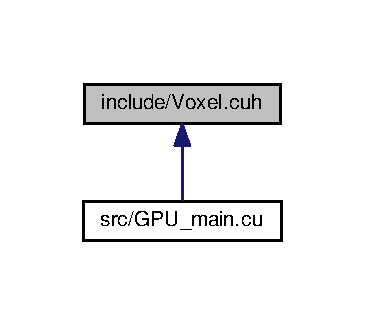
\includegraphics[width=175pt]{Voxel_8cuh__dep__incl}
\end{center}
\end{figure}
\subsubsection*{Classes}
\begin{DoxyCompactItemize}
\item 
class \hyperlink{classquaternion}{quaternion}
\begin{DoxyCompactList}\small\item\em A basic Quaternion class. \end{DoxyCompactList}\item 
struct \hyperlink{structPose}{Pose}
\begin{DoxyCompactList}\small\item\em \hyperlink{structPose}{Pose} of T265 camera. \end{DoxyCompactList}\item 
struct \hyperlink{structCam}{Cam}
\begin{DoxyCompactList}\small\item\em \hyperlink{classCamera}{Camera} Intrinsics and Extrinsics. \end{DoxyCompactList}\item 
struct \hyperlink{structTuple}{Tuple}
\begin{DoxyCompactList}\small\item\em Point co-\/ordinates and variance \end{DoxyCompactList}\item 
struct \hyperlink{structPoint}{Point}
\begin{DoxyCompactList}\small\item\em \hyperlink{structPoint}{Point} co-\/ordinates. \end{DoxyCompactList}\item 
class \hyperlink{classleaf}{leaf}
\begin{DoxyCompactList}\small\item\em Leaf nodes of the Octree structure. \end{DoxyCompactList}\item 
class \hyperlink{classvoxel}{voxel}
\begin{DoxyCompactList}\small\item\em Voxel/\+Intermediate nodes of the Octree structure. \end{DoxyCompactList}\item 
class \hyperlink{classGPU__FE}{G\+P\+U\+\_\+\+FE}
\begin{DoxyCompactList}\small\item\em Wrapper class for \hyperlink{classocc__grid}{occ\+\_\+grid}. \end{DoxyCompactList}\end{DoxyCompactItemize}
\subsubsection*{Macros}
\begin{DoxyCompactItemize}
\item 
\#define \hyperlink{Voxel_8cuh_aca76098e63473a0423c740cd04ec72b8}{V\+O\+X\+E\+L\+\_\+\+CH}
\item 
\#define \hyperlink{Voxel_8cuh_a29d8f4bb35f9fa62e1d680bc6ab1f4f1}{M\+I\+N\+\_\+L}~0.\+04
\begin{DoxyCompactList}\small\item\em Minimum dimension of leaf node. \end{DoxyCompactList}\item 
\#define \hyperlink{Voxel_8cuh_a3c1c8b966e30fa8ca2de07abe3b3d74a}{V\+O\+X\+\_\+L}~2.\+56
\begin{DoxyCompactList}\small\item\em Size of root voxels. \end{DoxyCompactList}\item 
\#define \hyperlink{Voxel_8cuh_ae1cd6283839fc3aebf9bccbd1044a365}{V\+A\+R\+\_\+P}~0.\+005
\begin{DoxyCompactList}\small\item\em Variance of measurement. \end{DoxyCompactList}\end{DoxyCompactItemize}
\begin{Indent}{\bf Kernel Launch Parameters}\par
\begin{DoxyCompactItemize}
\item 
\#define \hyperlink{Voxel_8cuh_a9f984157d0b56c37dfb4bd1a16f1e8ab}{N\+U\+M\+\_\+B}~480
\begin{DoxyCompactList}\small\item\em Number of blocks launched in the grid. \end{DoxyCompactList}\item 
\#define \hyperlink{Voxel_8cuh_ad8ba90b2d681fcfbc6cde44271ad6519}{N\+U\+M\+\_\+T}~640
\begin{DoxyCompactList}\small\item\em Number of threads launched in each block. \end{DoxyCompactList}\end{DoxyCompactItemize}
\end{Indent}
\subsubsection*{Functions}
\begin{DoxyCompactItemize}
\item 
void \hyperlink{Voxel_8cuh_af3f284d9dc439df44497e0e24b6d1fed}{gpu\+Assert} (cuda\+Error\+\_\+t code, const char $\ast$file, int line, bool abort=false)
\begin{DoxyCompactList}\small\item\em Prints out errors in C\+U\+DA kernel execution. \end{DoxyCompactList}\item 
void \hyperlink{Voxel_8cuh_aa881629585a7719857d28b2cbf1e1257}{gpu\+Check\+Kernel\+Execution\+Error} (const char $\ast$file, int line)
\begin{DoxyCompactList}\small\item\em Method to print out errors in C\+U\+DA kernel execution. \end{DoxyCompactList}\item 
\+\_\+\+\_\+device\+\_\+\+\_\+ \hyperlink{classPair}{Pair}$<$ long, \hyperlink{classPair}{Pair}$<$ \hyperlink{classvoxel}{voxel} $\ast$, \hyperlink{structPoint}{Point} $>$ $>$ \hyperlink{Voxel_8cuh_a8af940c50e32ce0514198b2bf835b80c}{binary\+\_\+search} (\hyperlink{classPair}{Pair}$<$ long, \hyperlink{classPair}{Pair}$<$ \hyperlink{classvoxel}{voxel} $\ast$, \hyperlink{structPoint}{Point} $>$ $>$ $\ast$v, long b, long e, long key)
\begin{DoxyCompactList}\small\item\em Binary search for key in sorted array. \end{DoxyCompactList}\item 
\+\_\+\+\_\+device\+\_\+\+\_\+ \hyperlink{structPoint}{Point} \hyperlink{Voxel_8cuh_abbd51b1d8c2bc9b7d5ef5413e1e4ca49}{mod\+\_\+p} (\hyperlink{structPoint}{Point} p)
\begin{DoxyCompactList}\small\item\em Calculates co-\/ordinate of point modulo edge length. \end{DoxyCompactList}\item 
\+\_\+\+\_\+device\+\_\+\+\_\+ long \hyperlink{Voxel_8cuh_afeed91d5a5a0b48801aca2d5edeaf3e1}{index} (\hyperlink{structPoint}{Point} p)
\begin{DoxyCompactList}\small\item\em Calculates index used as key to index into device vector. \end{DoxyCompactList}\item 
\+\_\+\+\_\+global\+\_\+\+\_\+ void \hyperlink{Voxel_8cuh_a935fc0c42796b23607cf6f81a1e95e8d}{Update\+\_\+root} (unsigned short d\mbox{[}\hyperlink{Camera_8hpp_a66326676d44c838441a4dc39c85f599b}{w} $\ast$\hyperlink{Camera_8hpp_a3f40fea9b1040e381f08ddd4b026765d}{h}\mbox{]}, \hyperlink{classPair}{Pair}$<$ long, \hyperlink{classPair}{Pair}$<$ \hyperlink{classvoxel}{voxel} $\ast$, \hyperlink{structPoint}{Point} $>$ $>$ $\ast$v, long $\ast$s, \hyperlink{classPair}{Pair}$<$ long, \hyperlink{classPair}{Pair}$<$ \hyperlink{classvoxel}{voxel} $\ast$, \hyperlink{structPoint}{Point} $>$ $>$ $\ast$temp, \hyperlink{structCam}{Cam} $\ast$c, \hyperlink{structPose}{Pose} $\ast$p)
\begin{DoxyCompactList}\small\item\em Updates point in the global map. \end{DoxyCompactList}\item 
\+\_\+\+\_\+global\+\_\+\+\_\+ void \hyperlink{Voxel_8cuh_afc844d313aa2b2353c757fb063b74b96}{Print} (\hyperlink{classPair}{Pair}$<$ long, \hyperlink{classPair}{Pair}$<$ \hyperlink{classvoxel}{voxel} $\ast$, \hyperlink{structPoint}{Point} $>$ $>$ $\ast$v, long $\ast$s, \hyperlink{structTuple}{Tuple} $\ast$set)
\begin{DoxyCompactList}\small\item\em Appends points to the vector of points. \end{DoxyCompactList}\end{DoxyCompactItemize}
\subsubsection*{Variables}
\begin{Indent}{\bf T265 to D435 extrinsics}\par
\begin{DoxyCompactItemize}
\item 
static const \hyperlink{classquaternion}{quaternion} \hyperlink{Voxel_8cuh_ae638036c15a578080c34013047df2c4f}{Q\+\_\+\+T265\+\_\+\+D435} (-\/0.\+0089999, 0.\+0024999, 0.\+0000225, 0.\+9999564)
\begin{DoxyCompactList}\small\item\em Quaternion from $\mathfrak{R}_{T265} \to \mathfrak{R}_{D435}$ in $\mathfrak{R}_{T265}$. \end{DoxyCompactList}\item 
static const \hyperlink{classquaternion}{quaternion} \hyperlink{Voxel_8cuh_a084c6bfb66f9daa4728fe8355861f1a4}{T\+\_\+\+T265\+\_\+\+D435} (0.\+021, 0.\+027, 0.\+009, 0)
\begin{DoxyCompactList}\small\item\em Translation from $\mathfrak{R}_{T265} \to \mathfrak{R}_{D435}$ in $\mathfrak{R}_{T265} (m)$. \end{DoxyCompactList}\end{DoxyCompactItemize}
\end{Indent}


\subsubsection{Macro Definition Documentation}
\index{Voxel.\+cuh@{Voxel.\+cuh}!M\+I\+N\+\_\+L@{M\+I\+N\+\_\+L}}
\index{M\+I\+N\+\_\+L@{M\+I\+N\+\_\+L}!Voxel.\+cuh@{Voxel.\+cuh}}
\paragraph[{\texorpdfstring{M\+I\+N\+\_\+L}{MIN_L}}]{\setlength{\rightskip}{0pt plus 5cm}\#define M\+I\+N\+\_\+L~0.\+04}\hypertarget{Voxel_8cuh_a29d8f4bb35f9fa62e1d680bc6ab1f4f1}{}\label{Voxel_8cuh_a29d8f4bb35f9fa62e1d680bc6ab1f4f1}


Minimum dimension of leaf node. 

The Voxels will keep dividing until their the size of voxel is $\leq$ M\+I\+N\+\_\+L, at which point a leaf is alloted in place of a voxel. Set the value as a floating value. eg\+: 1.\+00 

Definition at line \hyperlink{Voxel_8cuh_source_l00030}{30} of file \hyperlink{Voxel_8cuh_source}{Voxel.\+cuh}.

\index{Voxel.\+cuh@{Voxel.\+cuh}!N\+U\+M\+\_\+B@{N\+U\+M\+\_\+B}}
\index{N\+U\+M\+\_\+B@{N\+U\+M\+\_\+B}!Voxel.\+cuh@{Voxel.\+cuh}}
\paragraph[{\texorpdfstring{N\+U\+M\+\_\+B}{NUM_B}}]{\setlength{\rightskip}{0pt plus 5cm}\#define N\+U\+M\+\_\+B~480}\hypertarget{Voxel_8cuh_a9f984157d0b56c37dfb4bd1a16f1e8ab}{}\label{Voxel_8cuh_a9f984157d0b56c37dfb4bd1a16f1e8ab}


Number of blocks launched in the grid. 

Note\+: Launch parameters should satisfy all constraints. Run device\+Query in C\+U\+DA samples to check device characteristics.

Should be less than maximum Grid size in all dimensions 

Definition at line \hyperlink{Voxel_8cuh_source_l00049}{49} of file \hyperlink{Voxel_8cuh_source}{Voxel.\+cuh}.

\index{Voxel.\+cuh@{Voxel.\+cuh}!N\+U\+M\+\_\+T@{N\+U\+M\+\_\+T}}
\index{N\+U\+M\+\_\+T@{N\+U\+M\+\_\+T}!Voxel.\+cuh@{Voxel.\+cuh}}
\paragraph[{\texorpdfstring{N\+U\+M\+\_\+T}{NUM_T}}]{\setlength{\rightskip}{0pt plus 5cm}\#define N\+U\+M\+\_\+T~640}\hypertarget{Voxel_8cuh_ad8ba90b2d681fcfbc6cde44271ad6519}{}\label{Voxel_8cuh_ad8ba90b2d681fcfbc6cde44271ad6519}


Number of threads launched in each block. 

Should be less than maximum Block size in all dimensions 

Definition at line \hyperlink{Voxel_8cuh_source_l00053}{53} of file \hyperlink{Voxel_8cuh_source}{Voxel.\+cuh}.

\index{Voxel.\+cuh@{Voxel.\+cuh}!V\+A\+R\+\_\+P@{V\+A\+R\+\_\+P}}
\index{V\+A\+R\+\_\+P@{V\+A\+R\+\_\+P}!Voxel.\+cuh@{Voxel.\+cuh}}
\paragraph[{\texorpdfstring{V\+A\+R\+\_\+P}{VAR_P}}]{\setlength{\rightskip}{0pt plus 5cm}\#define V\+A\+R\+\_\+P~0.\+005}\hypertarget{Voxel_8cuh_ae1cd6283839fc3aebf9bccbd1044a365}{}\label{Voxel_8cuh_ae1cd6283839fc3aebf9bccbd1044a365}


Variance of measurement. 

This is the 3-\/D variance of each point measured. Assumed constant and isotropic. The co-\/variance matrix in this case is $ VAR\_P . \mathbb{1}_{3{\times}3} $ 

Definition at line \hyperlink{Voxel_8cuh_source_l00040}{40} of file \hyperlink{Voxel_8cuh_source}{Voxel.\+cuh}.

\index{Voxel.\+cuh@{Voxel.\+cuh}!V\+O\+X\+\_\+L@{V\+O\+X\+\_\+L}}
\index{V\+O\+X\+\_\+L@{V\+O\+X\+\_\+L}!Voxel.\+cuh@{Voxel.\+cuh}}
\paragraph[{\texorpdfstring{V\+O\+X\+\_\+L}{VOX_L}}]{\setlength{\rightskip}{0pt plus 5cm}\#define V\+O\+X\+\_\+L~2.\+56}\hypertarget{Voxel_8cuh_a3c1c8b966e30fa8ca2de07abe3b3d74a}{}\label{Voxel_8cuh_a3c1c8b966e30fa8ca2de07abe3b3d74a}


Size of root voxels. 

The starting size of root voxels. This should not be $\leq$ M\+I\+N\+\_\+L. Set the value as a floating value. eg\+: 3.\+00 

Definition at line \hyperlink{Voxel_8cuh_source_l00035}{35} of file \hyperlink{Voxel_8cuh_source}{Voxel.\+cuh}.

\index{Voxel.\+cuh@{Voxel.\+cuh}!V\+O\+X\+E\+L\+\_\+\+CH@{V\+O\+X\+E\+L\+\_\+\+CH}}
\index{V\+O\+X\+E\+L\+\_\+\+CH@{V\+O\+X\+E\+L\+\_\+\+CH}!Voxel.\+cuh@{Voxel.\+cuh}}
\paragraph[{\texorpdfstring{V\+O\+X\+E\+L\+\_\+\+CH}{VOXEL_CH}}]{\setlength{\rightskip}{0pt plus 5cm}\#define V\+O\+X\+E\+L\+\_\+\+CH}\hypertarget{Voxel_8cuh_aca76098e63473a0423c740cd04ec72b8}{}\label{Voxel_8cuh_aca76098e63473a0423c740cd04ec72b8}


Definition at line \hyperlink{Voxel_8cuh_source_l00002}{2} of file \hyperlink{Voxel_8cuh_source}{Voxel.\+cuh}.



\subsubsection{Function Documentation}
\index{Voxel.\+cuh@{Voxel.\+cuh}!binary\+\_\+search@{binary\+\_\+search}}
\index{binary\+\_\+search@{binary\+\_\+search}!Voxel.\+cuh@{Voxel.\+cuh}}
\paragraph[{\texorpdfstring{binary\+\_\+search(\+Pair$<$ long, Pair$<$ voxel $\ast$, Point $>$ $>$ $\ast$v, long b, long e, long key)}{binary_search(Pair< long, Pair< voxel *, Point > > *v, long b, long e, long key)}}]{\setlength{\rightskip}{0pt plus 5cm}\+\_\+\+\_\+device\+\_\+\+\_\+ {\bf Pair}$<$ long, {\bf Pair}$<${\bf voxel} $\ast$, {\bf Point}$>$ $>$ binary\+\_\+search (
\begin{DoxyParamCaption}
\item[{{\bf Pair}$<$ long, {\bf Pair}$<$ {\bf voxel} $\ast$, {\bf Point} $>$ $>$ $\ast$}]{v, }
\item[{long}]{b, }
\item[{long}]{e, }
\item[{long}]{key}
\end{DoxyParamCaption}
)}\hypertarget{Voxel_8cuh_a8af940c50e32ce0514198b2bf835b80c}{}\label{Voxel_8cuh_a8af940c50e32ce0514198b2bf835b80c}


Binary search for key in sorted array. 

Pointer to a sorted vector (stored in device) is passed along with the size and the starting index, and the binary search algorithm is used to index via key. It is a recursive method. 
\begin{DoxyParams}{Parameters}
{\em Pointer} & to sorted vector v, beginning index b, ending index e \\
\hline
{\em key} & ot index into vector \\
\hline
\end{DoxyParams}
\begin{DoxyReturn}{Returns}
\hyperlink{classPair}{Pair} of index and voxel with the given index 
\end{DoxyReturn}
\begin{DoxySeeAlso}{See also}
\hyperlink{Voxel_8cuh_a935fc0c42796b23607cf6f81a1e95e8d}{Update\+\_\+root()} 
\end{DoxySeeAlso}


Definition at line \hyperlink{Voxel_8cuh_source_l00475}{475} of file \hyperlink{Voxel_8cuh_source}{Voxel.\+cuh}.



Here is the caller graph for this function\+:\nopagebreak
\begin{figure}[H]
\begin{center}
\leavevmode
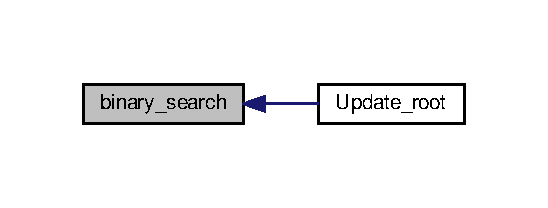
\includegraphics[width=263pt]{Voxel_8cuh_a8af940c50e32ce0514198b2bf835b80c_icgraph}
\end{center}
\end{figure}


\index{Voxel.\+cuh@{Voxel.\+cuh}!gpu\+Assert@{gpu\+Assert}}
\index{gpu\+Assert@{gpu\+Assert}!Voxel.\+cuh@{Voxel.\+cuh}}
\paragraph[{\texorpdfstring{gpu\+Assert(cuda\+Error\+\_\+t code, const char $\ast$file, int line, bool abort=false)}{gpuAssert(cudaError_t code, const char *file, int line, bool abort=false)}}]{\setlength{\rightskip}{0pt plus 5cm}void gpu\+Assert (
\begin{DoxyParamCaption}
\item[{cuda\+Error\+\_\+t}]{code, }
\item[{const char $\ast$}]{file, }
\item[{int}]{line, }
\item[{bool}]{abort = {\ttfamily false}}
\end{DoxyParamCaption}
)\hspace{0.3cm}{\ttfamily [inline]}}\hypertarget{Voxel_8cuh_af3f284d9dc439df44497e0e24b6d1fed}{}\label{Voxel_8cuh_af3f284d9dc439df44497e0e24b6d1fed}


Prints out errors in C\+U\+DA kernel execution. 



Definition at line \hyperlink{Voxel_8cuh_source_l00196}{196} of file \hyperlink{Voxel_8cuh_source}{Voxel.\+cuh}.



Here is the caller graph for this function\+:\nopagebreak
\begin{figure}[H]
\begin{center}
\leavevmode
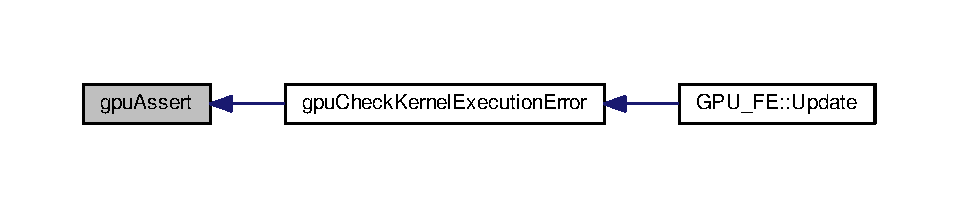
\includegraphics[width=350pt]{Voxel_8cuh_af3f284d9dc439df44497e0e24b6d1fed_icgraph}
\end{center}
\end{figure}


\index{Voxel.\+cuh@{Voxel.\+cuh}!gpu\+Check\+Kernel\+Execution\+Error@{gpu\+Check\+Kernel\+Execution\+Error}}
\index{gpu\+Check\+Kernel\+Execution\+Error@{gpu\+Check\+Kernel\+Execution\+Error}!Voxel.\+cuh@{Voxel.\+cuh}}
\paragraph[{\texorpdfstring{gpu\+Check\+Kernel\+Execution\+Error(const char $\ast$file, int line)}{gpuCheckKernelExecutionError(const char *file, int line)}}]{\setlength{\rightskip}{0pt plus 5cm}void gpu\+Check\+Kernel\+Execution\+Error (
\begin{DoxyParamCaption}
\item[{const char $\ast$}]{file, }
\item[{int}]{line}
\end{DoxyParamCaption}
)\hspace{0.3cm}{\ttfamily [inline]}}\hypertarget{Voxel_8cuh_aa881629585a7719857d28b2cbf1e1257}{}\label{Voxel_8cuh_aa881629585a7719857d28b2cbf1e1257}


Method to print out errors in C\+U\+DA kernel execution. 



Definition at line \hyperlink{Voxel_8cuh_source_l00207}{207} of file \hyperlink{Voxel_8cuh_source}{Voxel.\+cuh}.



Here is the call graph for this function\+:\nopagebreak
\begin{figure}[H]
\begin{center}
\leavevmode
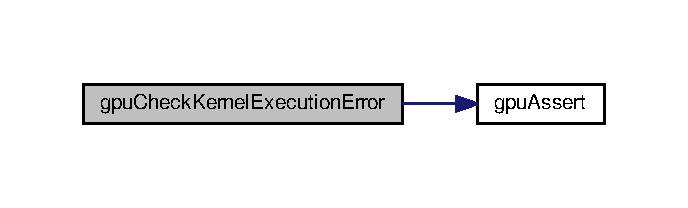
\includegraphics[width=330pt]{Voxel_8cuh_aa881629585a7719857d28b2cbf1e1257_cgraph}
\end{center}
\end{figure}




Here is the caller graph for this function\+:\nopagebreak
\begin{figure}[H]
\begin{center}
\leavevmode
\includegraphics[width=350pt]{Voxel_8cuh_aa881629585a7719857d28b2cbf1e1257_icgraph}
\end{center}
\end{figure}


\index{Voxel.\+cuh@{Voxel.\+cuh}!index@{index}}
\index{index@{index}!Voxel.\+cuh@{Voxel.\+cuh}}
\paragraph[{\texorpdfstring{index(\+Point p)}{index(Point p)}}]{\setlength{\rightskip}{0pt plus 5cm}\+\_\+\+\_\+device\+\_\+\+\_\+ long index (
\begin{DoxyParamCaption}
\item[{{\bf Point}}]{p}
\end{DoxyParamCaption}
)}\hypertarget{Voxel_8cuh_afeed91d5a5a0b48801aca2d5edeaf3e1}{}\label{Voxel_8cuh_afeed91d5a5a0b48801aca2d5edeaf3e1}


Calculates index used as key to index into device vector. 

This is used to calculate a unique whole number from a set of three integers\+: indices of origin of the voxel. Instead of using three nested maps each trying to index one co-\/ordinate at each level ( $ O(\ln(N_x)+\ln(N_y)+\ln(N_z))$), a bijective mapping from $ \mathbb{Z}^{3} \to \mathbb{N}$ is defined. Although the order of the complexity remains the same, the look-\/up is guaranteed to occur in less time than the previous case. 
\begin{DoxyParams}{Parameters}
{\em co-\/ordinates} & of the origin of voxel \\
\hline
\end{DoxyParams}
\begin{DoxyReturn}{Returns}
index of point 
\end{DoxyReturn}
\begin{DoxySeeAlso}{See also}
\hyperlink{classocc__grid_a0fb045d82217675decfc9b9289ad35ea}{occ\+\_\+grid\+::index()}, \hyperlink{classGPU__FE_aa9039bd613961d4e0911b8514ed14fba}{G\+P\+U\+\_\+\+F\+E\+::\+Update()} 
\end{DoxySeeAlso}


Definition at line \hyperlink{Voxel_8cuh_source_l00507}{507} of file \hyperlink{Voxel_8cuh_source}{Voxel.\+cuh}.



Here is the call graph for this function\+:\nopagebreak
\begin{figure}[H]
\begin{center}
\leavevmode
\includegraphics[width=202pt]{Voxel_8cuh_afeed91d5a5a0b48801aca2d5edeaf3e1_cgraph}
\end{center}
\end{figure}




Here is the caller graph for this function\+:\nopagebreak
\begin{figure}[H]
\begin{center}
\leavevmode
\includegraphics[width=350pt]{Voxel_8cuh_afeed91d5a5a0b48801aca2d5edeaf3e1_icgraph}
\end{center}
\end{figure}


\index{Voxel.\+cuh@{Voxel.\+cuh}!mod\+\_\+p@{mod\+\_\+p}}
\index{mod\+\_\+p@{mod\+\_\+p}!Voxel.\+cuh@{Voxel.\+cuh}}
\paragraph[{\texorpdfstring{mod\+\_\+p(\+Point p)}{mod_p(Point p)}}]{\setlength{\rightskip}{0pt plus 5cm}\+\_\+\+\_\+device\+\_\+\+\_\+ {\bf Point} mod\+\_\+p (
\begin{DoxyParamCaption}
\item[{{\bf Point}}]{p}
\end{DoxyParamCaption}
)}\hypertarget{Voxel_8cuh_abbd51b1d8c2bc9b7d5ef5413e1e4ca49}{}\label{Voxel_8cuh_abbd51b1d8c2bc9b7d5ef5413e1e4ca49}


Calculates co-\/ordinate of point modulo edge length. 

Returns $p mod VOX\_L[0, 1)^3$ 
\begin{DoxyParams}{Parameters}
{\em co-\/ordinate} & of point \\
\hline
\end{DoxyParams}
\begin{DoxyReturn}{Returns}
modulo of co-\/ordinate of point 
\end{DoxyReturn}
\begin{DoxySeeAlso}{See also}
\hyperlink{classocc__grid_abf7ece8bcafa68e1292b0be52a5d9996}{occ\+\_\+grid\+::mod\+\_\+p()} 
\end{DoxySeeAlso}


Definition at line \hyperlink{Voxel_8cuh_source_l00495}{495} of file \hyperlink{Voxel_8cuh_source}{Voxel.\+cuh}.



Here is the caller graph for this function\+:\nopagebreak
\begin{figure}[H]
\begin{center}
\leavevmode
\includegraphics[width=350pt]{Voxel_8cuh_abbd51b1d8c2bc9b7d5ef5413e1e4ca49_icgraph}
\end{center}
\end{figure}


\index{Voxel.\+cuh@{Voxel.\+cuh}!Print@{Print}}
\index{Print@{Print}!Voxel.\+cuh@{Voxel.\+cuh}}
\paragraph[{\texorpdfstring{Print(\+Pair$<$ long, Pair$<$ voxel $\ast$, Point $>$ $>$ $\ast$v, long $\ast$s, Tuple $\ast$set)}{Print(Pair< long, Pair< voxel *, Point > > *v, long *s, Tuple *set)}}]{\setlength{\rightskip}{0pt plus 5cm}\+\_\+\+\_\+global\+\_\+\+\_\+ void Print (
\begin{DoxyParamCaption}
\item[{{\bf Pair}$<$ long, {\bf Pair}$<$ {\bf voxel} $\ast$, {\bf Point} $>$ $>$ $\ast$}]{v, }
\item[{long $\ast$}]{s, }
\item[{{\bf Tuple} $\ast$}]{set}
\end{DoxyParamCaption}
)}\hypertarget{Voxel_8cuh_afc844d313aa2b2353c757fb063b74b96}{}\label{Voxel_8cuh_afc844d313aa2b2353c757fb063b74b96}


Appends points to the vector of points. 

This method recursively calls \hyperlink{classvoxel_a4189fb0f24ad9eba1447e2ebf8ee0015}{voxel\+::all\+\_\+points()}, to append all the points in the leaf nodes to the vector. This method is called from \hyperlink{classGPU__FE_aea86626bdab826bc91b955ad6e5f6653}{G\+P\+U\+\_\+\+F\+E\+::\+Points()} Run by a single C\+U\+DA thread, since it is called only once and doesn\textquotesingle{}t affect the performance. 
\begin{DoxyParams}{Parameters}
{\em vector} & of root voxels \\
\hline
{\em size} & of the voxel \\
\hline
{\em \hyperlink{structTuple}{Tuple}} & to store points \\
\hline
\end{DoxyParams}
\begin{DoxySeeAlso}{See also}
\hyperlink{classvoxel_a4189fb0f24ad9eba1447e2ebf8ee0015}{voxel\+::all\+\_\+points()}, \hyperlink{classGPU__FE_aea86626bdab826bc91b955ad6e5f6653}{G\+P\+U\+\_\+\+F\+E\+::\+Points()} 
\end{DoxySeeAlso}


Definition at line \hyperlink{Voxel_8cuh_source_l00589}{589} of file \hyperlink{Voxel_8cuh_source}{Voxel.\+cuh}.

\index{Voxel.\+cuh@{Voxel.\+cuh}!Update\+\_\+root@{Update\+\_\+root}}
\index{Update\+\_\+root@{Update\+\_\+root}!Voxel.\+cuh@{Voxel.\+cuh}}
\paragraph[{\texorpdfstring{Update\+\_\+root(unsigned short d[w $\ast$h], Pair$<$ long, Pair$<$ voxel $\ast$, Point $>$ $>$ $\ast$v, long $\ast$s, Pair$<$ long, Pair$<$ voxel $\ast$, Point $>$ $>$ $\ast$temp, Cam $\ast$c, Pose $\ast$p)}{Update_root(unsigned short d[w *h], Pair< long, Pair< voxel *, Point > > *v, long *s, Pair< long, Pair< voxel *, Point > > *temp, Cam *c, Pose *p)}}]{\setlength{\rightskip}{0pt plus 5cm}\+\_\+\+\_\+global\+\_\+\+\_\+ void Update\+\_\+root (
\begin{DoxyParamCaption}
\item[{unsigned short}]{d\mbox{[}w $\ast$h\mbox{]}, }
\item[{{\bf Pair}$<$ long, {\bf Pair}$<$ {\bf voxel} $\ast$, {\bf Point} $>$ $>$ $\ast$}]{v, }
\item[{long $\ast$}]{s, }
\item[{{\bf Pair}$<$ long, {\bf Pair}$<$ {\bf voxel} $\ast$, {\bf Point} $>$ $>$ $\ast$}]{temp, }
\item[{{\bf Cam} $\ast$}]{c, }
\item[{{\bf Pose} $\ast$}]{p}
\end{DoxyParamCaption}
)}\hypertarget{Voxel_8cuh_a935fc0c42796b23607cf6f81a1e95e8d}{}\label{Voxel_8cuh_a935fc0c42796b23607cf6f81a1e95e8d}


Updates point in the global map. 

This method recursively calls \hyperlink{classvoxel_a97737aec7c381e72d929d2f084952683}{voxel\+::update\+\_\+vox()} on multiple threads concurrently, to update the point in the respective voxel. This G\+PU kernel itself is called upon by \hyperlink{classGPU__FE_aa9039bd613961d4e0911b8514ed14fba}{G\+P\+U\+\_\+\+F\+E\+::\+Update()}. The information on the origin of the voxel is used to identify the voxel, and the index is used as a key to search in the sorted device vector. This method is the same as \hyperlink{classvoxel_a97737aec7c381e72d929d2f084952683}{voxel\+::update\+\_\+vox()}, other than the fact that the point doesn\textquotesingle{}t directly map to any \char`\"{}child\char`\"{} voxel. The co-\/ordinates are transformed from the D435 frame to T265 global frame and then passed on to \hyperlink{classocc__grid_aaf38d339d7d1b3226d9673f8d6102b2c}{occ\+\_\+grid\+::update\+\_\+point()}. Equivalent to \hyperlink{classocc__grid_aaf38d339d7d1b3226d9673f8d6102b2c}{occ\+\_\+grid\+::update\+\_\+point()}, and \hyperlink{classCPU__FE_aae7cb60a405b294a680a929ecff5c2ae}{C\+P\+U\+\_\+\+F\+E\+::\+Update()}. Since inserts and searches into the device vector would have to be done atomically, a temporary array of voxel pointers is used. The size of the array is fixed, and is calculated using D435 intrinsics, D435\+\_\+\+M\+AX, and V\+O\+X\+\_\+L, such that a mapping from each point to the array index can be made. Therefore, every point belonging to the same voxel is mapped to the same index in the array, which can be known. This not only solves the problem of consistency, but also results in almost maximum possible parallel efficiency. This temporary array is appended to the device vector containing root voxels, and is sorted (\hyperlink{classGPU__FE_aa9039bd613961d4e0911b8514ed14fba}{G\+P\+U\+\_\+\+F\+E\+::\+Update()}). Although sorting a vector, which is a linear array, takes $O(n)$ as opposed to the $O(\ln(n))$ for insertion in a map, which is a red-\/black tree, since new voxels are sparsely created, it is not expected to reduce performance noticeably. This difference in insertion times can be attributed ot the fact that indexing in a linear array is $O(1)$. 
\begin{DoxyParams}{Parameters}
{\em \hyperlink{classCamera}{Camera}} & object \\
\hline
{\em pose} & of T265 \\
\hline
{\em 16-\/bit} & D435 depth image \\
\hline
{\em device} & vector containing root voxel pointers \\
\hline
{\em size} & of device vector \\
\hline
\end{DoxyParams}
\begin{DoxySeeAlso}{See also}
\hyperlink{classvoxel_a97737aec7c381e72d929d2f084952683}{voxel\+::update\+\_\+vox()}, \hyperlink{classGPU__FE_aa9039bd613961d4e0911b8514ed14fba}{G\+P\+U\+\_\+\+F\+E\+::\+Update()} 
\end{DoxySeeAlso}


Definition at line \hyperlink{Voxel_8cuh_source_l00536}{536} of file \hyperlink{Voxel_8cuh_source}{Voxel.\+cuh}.



Here is the call graph for this function\+:\nopagebreak
\begin{figure}[H]
\begin{center}
\leavevmode
\includegraphics[width=350pt]{Voxel_8cuh_a935fc0c42796b23607cf6f81a1e95e8d_cgraph}
\end{center}
\end{figure}




\subsubsection{Variable Documentation}
\index{Voxel.\+cuh@{Voxel.\+cuh}!Q\+\_\+\+T265\+\_\+\+D435@{Q\+\_\+\+T265\+\_\+\+D435}}
\index{Q\+\_\+\+T265\+\_\+\+D435@{Q\+\_\+\+T265\+\_\+\+D435}!Voxel.\+cuh@{Voxel.\+cuh}}
\paragraph[{\texorpdfstring{Q\+\_\+\+T265\+\_\+\+D435}{Q_T265_D435}}]{\setlength{\rightskip}{0pt plus 5cm}const {\bf quaternion} Q\+\_\+\+T265\+\_\+\+D435(-\/0.\+0089999, 0.\+0024999, 0.\+0000225, 0.\+9999564)\hspace{0.3cm}{\ttfamily [static]}}\hypertarget{Voxel_8cuh_ae638036c15a578080c34013047df2c4f}{}\label{Voxel_8cuh_ae638036c15a578080c34013047df2c4f}


Quaternion from $\mathfrak{R}_{T265} \to \mathfrak{R}_{D435}$ in $\mathfrak{R}_{T265}$. 

To be obtained from extrinsic calibration data of the mount. \index{Voxel.\+cuh@{Voxel.\+cuh}!T\+\_\+\+T265\+\_\+\+D435@{T\+\_\+\+T265\+\_\+\+D435}}
\index{T\+\_\+\+T265\+\_\+\+D435@{T\+\_\+\+T265\+\_\+\+D435}!Voxel.\+cuh@{Voxel.\+cuh}}
\paragraph[{\texorpdfstring{T\+\_\+\+T265\+\_\+\+D435}{T_T265_D435}}]{\setlength{\rightskip}{0pt plus 5cm}const {\bf quaternion} T\+\_\+\+T265\+\_\+\+D435(0.\+021, 0.\+027, 0.\+009, 0)\hspace{0.3cm}{\ttfamily [static]}}\hypertarget{Voxel_8cuh_a084c6bfb66f9daa4728fe8355861f1a4}{}\label{Voxel_8cuh_a084c6bfb66f9daa4728fe8355861f1a4}


Translation from $\mathfrak{R}_{T265} \to \mathfrak{R}_{D435}$ in $\mathfrak{R}_{T265} (m)$. 


\hypertarget{Voxel_8cuh_source}{}\subsection{Voxel.\+cuh}
\label{Voxel_8cuh_source}\index{include/\+Voxel.\+cuh@{include/\+Voxel.\+cuh}}

\begin{DoxyCode}
00001 \textcolor{preprocessor}{#ifndef VOXEL\_CH}
\hypertarget{Voxel_8cuh_source.tex_l00002}{}\hyperlink{Voxel_8cuh_aca76098e63473a0423c740cd04ec72b8}{00002} \textcolor{preprocessor}{#define VOXEL\_CH}
00003 
00004 
00005 \textcolor{preprocessor}{#include <cuda.h>}
00006 \textcolor{preprocessor}{#include <cuda\_runtime.h>}
00007 \textcolor{preprocessor}{#include <cuda\_profiler\_api.h>}
00008 
00009 \textcolor{preprocessor}{#include <iostream>}
00010 \textcolor{preprocessor}{#include <fstream>}
00011 
00012 \textcolor{preprocessor}{#include <typeinfo>}
00013 \textcolor{preprocessor}{#include <cmath>}
00014 \textcolor{preprocessor}{#include <math.h>}
00015 \textcolor{preprocessor}{#include <utility>}
00016 \textcolor{preprocessor}{#include <unistd.h>}
00017 \textcolor{preprocessor}{#include <thrust/tuple.h>}
00018 \textcolor{preprocessor}{#include <thrust/host\_vector.h>}
00019 \textcolor{preprocessor}{#include <thrust/device\_vector.h>}
00020 \textcolor{preprocessor}{#include <thrust/execution\_policy.h>}
00021 \textcolor{preprocessor}{#include <thrust/sort.h>}
00022 \textcolor{preprocessor}{#include <thrust/binary\_search.h>}
00023 
00024 \textcolor{preprocessor}{#include "\hyperlink{Helper_8hpp}{Helper.hpp}"}
00025 
00027 
\hypertarget{Voxel_8cuh_source.tex_l00030}{}\hyperlink{Voxel_8cuh_a29d8f4bb35f9fa62e1d680bc6ab1f4f1}{00030} \textcolor{preprocessor}{#define MIN\_L 0.04 // minimum edge length of leaf in meter}
00031 
\hypertarget{Voxel_8cuh_source.tex_l00035}{}\hyperlink{Voxel_8cuh_a3c1c8b966e30fa8ca2de07abe3b3d74a}{00035} \textcolor{preprocessor}{#define VOX\_L 2.56 // edge length of root voxel in meter (>= MIN\_L). Define as float:eg: 2.00}
00036 
\hypertarget{Voxel_8cuh_source.tex_l00040}{}\hyperlink{Voxel_8cuh_ae1cd6283839fc3aebf9bccbd1044a365}{00040} \textcolor{preprocessor}{#define VAR\_P 0.005 // variance of each measurement}
00041 
00044 
00047 
\hypertarget{Voxel_8cuh_source.tex_l00049}{}\hyperlink{Voxel_8cuh_a9f984157d0b56c37dfb4bd1a16f1e8ab}{00049} \textcolor{preprocessor}{#define NUM\_B 480}
00050 
\hypertarget{Voxel_8cuh_source.tex_l00053}{}\hyperlink{Voxel_8cuh_ad8ba90b2d681fcfbc6cde44271ad6519}{00053} \textcolor{preprocessor}{#define NUM\_T 640}
00054 
00056 
00058 
\hypertarget{Voxel_8cuh_source.tex_l00063}{}\hyperlink{classquaternion}{00063} \textcolor{keyword}{class }\hyperlink{classquaternion}{quaternion} \{
00064 
00065 \textcolor{keyword}{public}:
00066 
\hypertarget{Voxel_8cuh_source.tex_l00069}{}\hyperlink{classquaternion_a538598007238d399f79ddcecd39ef5cf}{00069}     \textcolor{keywordtype}{float} \hyperlink{classquaternion_acdcda48f9dd7ff35873aae38fa33ab78}{x}, \hyperlink{classquaternion_a48e3d1fbf5e12eb54985c32b45dd8303}{y}, \hyperlink{classquaternion_a538598007238d399f79ddcecd39ef5cf}{z}, \hyperlink{classquaternion_ab2b38aca1971114e0ba4218b75d7f472}{w};
00071 
00073 
\hypertarget{Voxel_8cuh_source.tex_l00077}{}\hyperlink{classquaternion_a01adb7930c2003b777cb91a7182c482e}{00077}     \_\_host\_\_ \_\_device\_\_ \hyperlink{classquaternion_a01adb7930c2003b777cb91a7182c482e}{quaternion} (\textcolor{keywordtype}{float} x, \textcolor{keywordtype}{float} y, \textcolor{keywordtype}{float} z, \textcolor{keywordtype}{float} w) \{
00078         this->x = \hyperlink{classquaternion_acdcda48f9dd7ff35873aae38fa33ab78}{x};
00079         this->y = \hyperlink{classquaternion_a48e3d1fbf5e12eb54985c32b45dd8303}{y};
00080         this->z = \hyperlink{classquaternion_a538598007238d399f79ddcecd39ef5cf}{z};
00081         this->w = \hyperlink{classquaternion_ab2b38aca1971114e0ba4218b75d7f472}{w};
00082     \}
00083 
00085 
\hypertarget{Voxel_8cuh_source.tex_l00088}{}\hyperlink{classquaternion_a5f2dff4e0f446d05e826a63d5a45d230}{00088}     \_\_host\_\_ \_\_device\_\_ \hyperlink{classquaternion}{quaternion} \hyperlink{classquaternion_a5f2dff4e0f446d05e826a63d5a45d230}{inv} () \{
00089         \textcolor{keywordtype}{float} l = (this->\hyperlink{classquaternion_acdcda48f9dd7ff35873aae38fa33ab78}{x})*(this->x) + (this->\hyperlink{classquaternion_a48e3d1fbf5e12eb54985c32b45dd8303}{y})*(this->y) + (this->\hyperlink{classquaternion_a538598007238d399f79ddcecd39ef5cf}{z})*(this->z) + (this->
      \hyperlink{classquaternion_ab2b38aca1971114e0ba4218b75d7f472}{w})*(this->w);
00090         \textcolor{keywordflow}{return} \hyperlink{classquaternion_a01adb7930c2003b777cb91a7182c482e}{quaternion} (-(this->x)/l, -(this->y)/l, -(this->z)/l, (this->w)/l);
00091     \}
00092 
00094     \textcolor{comment}{/*  To be used as \(\backslash\)f$q\_1*q\_2\(\backslash\)f$ \(\backslash\)f$\(\backslash\)equiv q\_1\(\backslash\)timesq\_2\(\backslash\)f$, where &\(\backslash\)f$q\_1\(\backslash\)f$ = this}
00095 \textcolor{comment}{    *   \(\backslash\)param \(\backslash\)f$q\_2\(\backslash\)f$}
00096 \textcolor{comment}{    *   \(\backslash\)return quaternion}
00097 \textcolor{comment}{    */}
\hypertarget{Voxel_8cuh_source.tex_l00098}{}\hyperlink{classquaternion_a63777bf9c0c0a269852808442c2be4f5}{00098}     \_\_host\_\_ \_\_device\_\_ \hyperlink{classquaternion}{quaternion} \hyperlink{classquaternion_a63777bf9c0c0a269852808442c2be4f5}{operator * }(\hyperlink{classquaternion}{quaternion} \textcolor{keyword}{const} &q) \{
00099         \hyperlink{classquaternion}{quaternion} q\_t(0, 0, 0, 0);
00100         q\_t.\hyperlink{classquaternion_acdcda48f9dd7ff35873aae38fa33ab78}{x} = + this->x*q.\hyperlink{classquaternion_ab2b38aca1971114e0ba4218b75d7f472}{w} + this->y*q.\hyperlink{classquaternion_a538598007238d399f79ddcecd39ef5cf}{z} - this->z*q.\hyperlink{classquaternion_a48e3d1fbf5e12eb54985c32b45dd8303}{y} + this->w*q.\hyperlink{classquaternion_acdcda48f9dd7ff35873aae38fa33ab78}{x};
00101         q\_t.\hyperlink{classquaternion_a48e3d1fbf5e12eb54985c32b45dd8303}{y} = - this->x*q.\hyperlink{classquaternion_a538598007238d399f79ddcecd39ef5cf}{z} + this->y*q.\hyperlink{classquaternion_ab2b38aca1971114e0ba4218b75d7f472}{w} + this->z*q.\hyperlink{classquaternion_acdcda48f9dd7ff35873aae38fa33ab78}{x} + this->w*q.\hyperlink{classquaternion_a48e3d1fbf5e12eb54985c32b45dd8303}{y};
00102         q\_t.\hyperlink{classquaternion_a538598007238d399f79ddcecd39ef5cf}{z} = + this->x*q.\hyperlink{classquaternion_a48e3d1fbf5e12eb54985c32b45dd8303}{y} - this->y*q.\hyperlink{classquaternion_acdcda48f9dd7ff35873aae38fa33ab78}{x} + this->z*q.\hyperlink{classquaternion_ab2b38aca1971114e0ba4218b75d7f472}{w} + this->w*q.\hyperlink{classquaternion_a538598007238d399f79ddcecd39ef5cf}{z};
00103         q\_t.\hyperlink{classquaternion_ab2b38aca1971114e0ba4218b75d7f472}{w} = - this->x*q.\hyperlink{classquaternion_acdcda48f9dd7ff35873aae38fa33ab78}{x} - this->y*q.\hyperlink{classquaternion_a48e3d1fbf5e12eb54985c32b45dd8303}{y} - this->z*q.\hyperlink{classquaternion_a538598007238d399f79ddcecd39ef5cf}{z} + this->w*q.\hyperlink{classquaternion_ab2b38aca1971114e0ba4218b75d7f472}{w};
00104         \textcolor{keywordflow}{return} q\_t;
00105     \}
00106 
00108     \textcolor{comment}{/*  To be used as \(\backslash\)f$q\_1+q\_2\(\backslash\)f$ \(\backslash\)f$\(\backslash\)equiv q\_1+q\_2\(\backslash\)f$, where &\(\backslash\)f$q\_1\(\backslash\)f$ = this}
00109 \textcolor{comment}{    *   \(\backslash\)param \(\backslash\)f$q\_2\(\backslash\)f$}
00110 \textcolor{comment}{    *   \(\backslash\)return quaternion}
00111 \textcolor{comment}{    */}
\hypertarget{Voxel_8cuh_source.tex_l00112}{}\hyperlink{classquaternion_ae2cf533c781610bf66bf39c30bd6b6ec}{00112}     \_\_host\_\_ \_\_device\_\_ \hyperlink{classquaternion}{quaternion} \hyperlink{classquaternion_ae2cf533c781610bf66bf39c30bd6b6ec}{operator + }(\hyperlink{classquaternion}{quaternion} \textcolor{keyword}{const} &q) \{
00113         \textcolor{keywordflow}{return} \hyperlink{classquaternion_a01adb7930c2003b777cb91a7182c482e}{quaternion} (this->x+q.\hyperlink{classquaternion_acdcda48f9dd7ff35873aae38fa33ab78}{x}, this->y+q.\hyperlink{classquaternion_a48e3d1fbf5e12eb54985c32b45dd8303}{y}, this->z+q.\hyperlink{classquaternion_a538598007238d399f79ddcecd39ef5cf}{z}, this->w+q.
      \hyperlink{classquaternion_ab2b38aca1971114e0ba4218b75d7f472}{w});
00114     \}
00115 \};
00116 
00118 
\hypertarget{Voxel_8cuh_source.tex_l00120}{}\hyperlink{structPose}{00120} \textcolor{keyword}{struct }\hyperlink{structPose}{Pose} \{
\hypertarget{Voxel_8cuh_source.tex_l00122}{}\hyperlink{structPose_aa87ab4baa5bab93b316c8ef417b6f1ef}{00122}     \hyperlink{classquaternion}{quaternion} \hyperlink{structPose_aa87ab4baa5bab93b316c8ef417b6f1ef}{t};
\hypertarget{Voxel_8cuh_source.tex_l00124}{}\hyperlink{structPose_ac86b5844a0203b03971005be99e59388}{00124}     \hyperlink{classquaternion}{quaternion} \hyperlink{structPose_ac86b5844a0203b03971005be99e59388}{r};
00125 \};
00126 
00128 
\hypertarget{Voxel_8cuh_source.tex_l00130}{}\hyperlink{structCam}{00130} \textcolor{keyword}{struct }\hyperlink{structCam}{Cam} \{
00131 
00134 
\hypertarget{Voxel_8cuh_source.tex_l00135}{}\hyperlink{structCam_a2c80b4688fa8d02ad6c645246b6ea0d4}{00135}     \textcolor{keywordtype}{float} fx, \hyperlink{structCam_a2c80b4688fa8d02ad6c645246b6ea0d4}{fy};   \textcolor{comment}{// |}
00137 \textcolor{comment}{}
00140 
\hypertarget{Voxel_8cuh_source.tex_l00141}{}\hyperlink{structCam_a5af4cee2ad3b008befb9626990dfbff2}{00141}     \textcolor{keywordtype}{float} ppx, \hyperlink{structCam_a5af4cee2ad3b008befb9626990dfbff2}{ppy}; \textcolor{comment}{// | - Camera intrinsics}
00143 \textcolor{comment}{}
\hypertarget{Voxel_8cuh_source.tex_l00145}{}\hyperlink{structCam_a99a4c54ed1a408665a0963f308008ec8}{00145}     \textcolor{keywordtype}{float} \hyperlink{structCam_a99a4c54ed1a408665a0963f308008ec8}{scale};    \textcolor{comment}{// |}
00146 
00149 
\hypertarget{Voxel_8cuh_source.tex_l00150}{}\hyperlink{structCam_a05f5a946647cd44a473b0fd03186ca96}{00150}     \hyperlink{classquaternion}{quaternion} Q\_TD, \hyperlink{structCam_a05f5a946647cd44a473b0fd03186ca96}{T\_TD}; \textcolor{comment}{// Camera extrinsics}
00152 \textcolor{comment}{}\};
00153 
00155 
\hypertarget{Voxel_8cuh_source.tex_l00157}{}\hyperlink{structTuple}{00157} \textcolor{keyword}{struct }\hyperlink{structTuple}{Tuple} \{
00158 
00161 
\hypertarget{Voxel_8cuh_source.tex_l00162}{}\hyperlink{structTuple_a5f83aeb6b110bc956fd27b8e713a9ad5}{00162}     \textcolor{keywordtype}{float} \hyperlink{classquaternion_acdcda48f9dd7ff35873aae38fa33ab78}{x}, \hyperlink{classquaternion_a48e3d1fbf5e12eb54985c32b45dd8303}{y}, \hyperlink{structTuple_a5f83aeb6b110bc956fd27b8e713a9ad5}{z};
00164 
\hypertarget{Voxel_8cuh_source.tex_l00166}{}\hyperlink{structTuple_a69871fb52122a48baa140565fb1b7c0c}{00166}     \textcolor{keywordtype}{float} \hyperlink{structTuple_a69871fb52122a48baa140565fb1b7c0c}{c};
00167 \};
00168 
00170 
\hypertarget{Voxel_8cuh_source.tex_l00172}{}\hyperlink{structPoint}{00172} \textcolor{keyword}{struct }\hyperlink{structPoint}{Point} \{
00173 
00176 
\hypertarget{Voxel_8cuh_source.tex_l00177}{}\hyperlink{structPoint_a9a666531e0e99adff132be93d2407d0c}{00177}     \textcolor{keywordtype}{float} \hyperlink{classquaternion_acdcda48f9dd7ff35873aae38fa33ab78}{x}, \hyperlink{classquaternion_a48e3d1fbf5e12eb54985c32b45dd8303}{y}, \hyperlink{structPoint_a9a666531e0e99adff132be93d2407d0c}{z};
00179 \};
00180 
00181 
00183 
00185 
00188 \textcolor{keyword}{static} \textcolor{keyword}{const} \hyperlink{classquaternion}{quaternion} \hyperlink{Voxel_8cuh_ae638036c15a578080c34013047df2c4f}{Q\_T265\_D435} (-0.0089999, 0.0024999, 0.0000225, 0.9999564); \textcolor{comment}{//
       | - T265 to D435 extrinsics}
00190 \textcolor{comment}{}\textcolor{keyword}{static} \textcolor{keyword}{const} \hyperlink{classquaternion}{quaternion} \hyperlink{Voxel_8cuh_a084c6bfb66f9daa4728fe8355861f1a4}{T\_T265\_D435} (0.021, 0.027, 0.009, 0);                      \textcolor{comment}{//
       |}
00192 \textcolor{comment}{}
00193 
00194 
\hypertarget{Voxel_8cuh_source.tex_l00196}{}\hyperlink{Voxel_8cuh_af3f284d9dc439df44497e0e24b6d1fed}{00196} \textcolor{keyword}{inline} \textcolor{keywordtype}{void} \hyperlink{Voxel_8cuh_af3f284d9dc439df44497e0e24b6d1fed}{gpuAssert}(cudaError\_t code, \textcolor{keyword}{const} \textcolor{keywordtype}{char} *file, \textcolor{keywordtype}{int} line, \textcolor{keywordtype}{bool} abort=\textcolor{keyword}{false})
00197 \{
00198     \textcolor{keywordflow}{if} (code != cudaSuccess) 
00199     \{
00200         fprintf(stderr,\textcolor{stringliteral}{"GPUassert: %s %s %d\(\backslash\)n"}, cudaGetErrorString(code), file, line);
00201         \textcolor{keywordflow}{if}( abort )
00202             exit(code);
00203     \}
00204 \}
00205 
\hypertarget{Voxel_8cuh_source.tex_l00207}{}\hyperlink{Voxel_8cuh_aa881629585a7719857d28b2cbf1e1257}{00207} \textcolor{keyword}{inline} \textcolor{keywordtype}{void} \hyperlink{Voxel_8cuh_aa881629585a7719857d28b2cbf1e1257}{gpuCheckKernelExecutionError}( \textcolor{keyword}{const} \textcolor{keywordtype}{char} *file, \textcolor{keywordtype}{int} line)
00208 \{
00209     \hyperlink{Voxel_8cuh_af3f284d9dc439df44497e0e24b6d1fed}{gpuAssert}( cudaPeekAtLastError(), file, line);
00210     \hyperlink{Voxel_8cuh_af3f284d9dc439df44497e0e24b6d1fed}{gpuAssert}( cudaDeviceSynchronize(), file, line);    
00211 \}
00212 
00213 
00214 \textcolor{comment}{/* leaf class */}
00216 
\hypertarget{Voxel_8cuh_source.tex_l00228}{}\hyperlink{classleaf}{00228} \textcolor{keyword}{class }\hyperlink{classleaf}{leaf} \{
00229 
00230 \textcolor{keyword}{public}:
00231 
00233 
\hypertarget{Voxel_8cuh_source.tex_l00239}{}\hyperlink{classleaf_a4fc347dbd4f5911bbb477910588ed512}{00239}     \textcolor{keywordtype}{float} \hyperlink{classleaf_a4fc347dbd4f5911bbb477910588ed512}{\_v};
00240 
00242 
00248 
\hypertarget{Voxel_8cuh_source.tex_l00250}{}\hyperlink{classleaf_a5f51fe13eb6e53bd9549469011e7a10e}{00250}     \textcolor{keywordtype}{float} x\_v, y\_v, \hyperlink{classleaf_a5f51fe13eb6e53bd9549469011e7a10e}{z\_v};
00252 
00254 
\hypertarget{Voxel_8cuh_source.tex_l00257}{}\hyperlink{classleaf_adfaf04cd4b50545cbc902d1aa36bc609}{00257}     \_\_device\_\_ \hyperlink{classleaf_adfaf04cd4b50545cbc902d1aa36bc609}{leaf} (\textcolor{keywordtype}{float} \hyperlink{classquaternion_acdcda48f9dd7ff35873aae38fa33ab78}{x}, \textcolor{keywordtype}{float} \hyperlink{classquaternion_a48e3d1fbf5e12eb54985c32b45dd8303}{y}, \textcolor{keywordtype}{float} \hyperlink{classquaternion_a538598007238d399f79ddcecd39ef5cf}{z}) \{ \textcolor{comment}{// state = -1: unoccupied}
00258         \_v = 0;
00259         x\_v = y\_v = z\_v = 0;
00260     \}
00261 
00263 
\hypertarget{Voxel_8cuh_source.tex_l00270}{}\hyperlink{classleaf_a3c205ce57e242832977bde6e1a04d7da}{00270}     \_\_device\_\_ \textcolor{keywordtype}{void} \hyperlink{classleaf_a3c205ce57e242832977bde6e1a04d7da}{update\_leaf} (\textcolor{keywordtype}{float} \hyperlink{classquaternion_acdcda48f9dd7ff35873aae38fa33ab78}{x}, \textcolor{keywordtype}{float} \hyperlink{classquaternion_a48e3d1fbf5e12eb54985c32b45dd8303}{y}, \textcolor{keywordtype}{float} \hyperlink{classquaternion_a538598007238d399f79ddcecd39ef5cf}{z}) \{ \textcolor{comment}{// x, y, z: scaled wrt to
       this->size}
00271         atomicAdd(&x\_v, x/\hyperlink{Voxel_8cuh_ae1cd6283839fc3aebf9bccbd1044a365}{VAR\_P});
00272         atomicAdd(&y\_v, y/\hyperlink{Voxel_8cuh_ae1cd6283839fc3aebf9bccbd1044a365}{VAR\_P});
00273         atomicAdd(&z\_v, z/\hyperlink{Voxel_8cuh_ae1cd6283839fc3aebf9bccbd1044a365}{VAR\_P});
00274         atomicAdd(&\_v, 1/\hyperlink{Voxel_8cuh_ae1cd6283839fc3aebf9bccbd1044a365}{VAR\_P});
00275     \}
00276 
00277 \};
00278 
00279 
00280 \textcolor{comment}{/* voxel class */}
00282 
\hypertarget{Voxel_8cuh_source.tex_l00297}{}\hyperlink{classvoxel}{00297} \textcolor{keyword}{class }\hyperlink{classvoxel}{voxel} \{
00298 
00299 \textcolor{keyword}{public}:
00300 
00302 
\hypertarget{Voxel_8cuh_source.tex_l00306}{}\hyperlink{classvoxel_aa280f71c0258d85ffef6f1818872a00a}{00306}     \textcolor{keywordtype}{void} * c[8]; \textcolor{comment}{// child voxels}
00308 \textcolor{comment}{}
\hypertarget{Voxel_8cuh_source.tex_l00313}{}\hyperlink{classvoxel_a01aebb82be393552c039c11a2c168845}{00313}     \textcolor{keywordtype}{float} \hyperlink{classvoxel_a01aebb82be393552c039c11a2c168845}{\_v}; \textcolor{comment}{// inverse of variance}
00314 
00316 
00321 
\hypertarget{Voxel_8cuh_source.tex_l00323}{}\hyperlink{classvoxel_a66addb3e42303e4a90a745c2174b0043}{00323}     \textcolor{keywordtype}{float} x\_v, y\_v, \hyperlink{classvoxel_a66addb3e42303e4a90a745c2174b0043}{z\_v}; \textcolor{comment}{// point co-ordinate wrt voxel (0-1) / variance}
\hypertarget{Voxel_8cuh_source.tex_l00326}{}\hyperlink{classvoxel_a573bae3d6e8383a4b2235d3cd33e7ab6}{00326} \textcolor{comment}{}    \textcolor{keywordtype}{float} \hyperlink{classvoxel_a573bae3d6e8383a4b2235d3cd33e7ab6}{size}; \textcolor{comment}{// edge length of voxel in meter}
00327     \textcolor{comment}{/* voxel * p; // parent voxel - initialize in constructor if used */}
00328 
00330 
\hypertarget{Voxel_8cuh_source.tex_l00334}{}\hyperlink{classvoxel_a1f832fd40f23c4fd721a4144387db6ef}{00334}     \_\_device\_\_ \hyperlink{classvoxel_a1f832fd40f23c4fd721a4144387db6ef}{voxel} (\textcolor{keywordtype}{float} \hyperlink{classquaternion_acdcda48f9dd7ff35873aae38fa33ab78}{x}, \textcolor{keywordtype}{float} \hyperlink{classquaternion_a48e3d1fbf5e12eb54985c32b45dd8303}{y}, \textcolor{keywordtype}{float} \hyperlink{classquaternion_a538598007238d399f79ddcecd39ef5cf}{z}, \textcolor{keywordtype}{float} size) \{ \textcolor{comment}{// state = -1: unoccupied}
00335         \_v = 0;
00336         x\_v = y\_v = z\_v = 0;
00337         this->size = size;
00338         c[0] = c[1] = c[2] = c[3] = c[4] = c[5] = c[6] = c[7] = NULL;
00339     \}
00340 
00342 
\hypertarget{Voxel_8cuh_source.tex_l00355}{}\hyperlink{classvoxel_a97737aec7c381e72d929d2f084952683}{00355}     \_\_device\_\_ \textcolor{keywordtype}{void} \hyperlink{classvoxel_a97737aec7c381e72d929d2f084952683}{update\_vox} (\textcolor{keywordtype}{float} \hyperlink{classquaternion_acdcda48f9dd7ff35873aae38fa33ab78}{x}, \textcolor{keywordtype}{float} \hyperlink{classquaternion_a48e3d1fbf5e12eb54985c32b45dd8303}{y}, \textcolor{keywordtype}{float} \hyperlink{classquaternion_a538598007238d399f79ddcecd39ef5cf}{z}) \{ \textcolor{comment}{// x, y, z: scaled wrt to
       this->size}
00356 
00357         \textcolor{comment}{/* update child voxels */}
00358         \textcolor{keywordtype}{int} idx = (z >= 0.5)<<2 | (y >= 0.5)<<1 | (x >= 0.5); \textcolor{comment}{// idx of child voxel the point lies in}
00359 
00360         \textcolor{keywordflow}{if} (size/4 >= \hyperlink{Voxel_8cuh_a29d8f4bb35f9fa62e1d680bc6ab1f4f1}{MIN\_L}) \{ \textcolor{comment}{/* child is a voxel object */}
00361             \textcolor{keywordflow}{if} (c[idx] == NULL) \{
00362                 \textcolor{keywordtype}{void} * cptr = (\textcolor{keywordtype}{void} *) \textcolor{keyword}{new} \hyperlink{classvoxel}{voxel} (fmodf(x,0.5)*2, fmodf(y,0.5)*2, fmodf(z,0.5)*2, size
      /2);
00363                 \textcolor{keywordflow}{if} ((\textcolor{keywordtype}{void} *)atomicCAS ((\textcolor{keywordtype}{unsigned} \textcolor{keywordtype}{long} \textcolor{keywordtype}{long} \textcolor{keywordtype}{int} *)&c[idx], (\textcolor{keywordtype}{unsigned} \textcolor{keywordtype}{long} \textcolor{keywordtype}{long} \textcolor{keywordtype}{int})NULL, (\textcolor{keywordtype}{
      unsigned} \textcolor{keywordtype}{long} \textcolor{keywordtype}{long} \textcolor{keywordtype}{int})cptr) != NULL) \textcolor{comment}{// child created by some other thread}
00364                     \textcolor{keyword}{delete} ((\hyperlink{classvoxel}{voxel} *)cptr);
00365                 ((\hyperlink{classvoxel}{voxel} *)c[idx])->\hyperlink{classvoxel_a1748472909af5ef1f28d0a0c6648dbbd}{update\_self}(fmodf(x,0.5)*2, fmodf(y,0.5)*2, fmodf(z,0.5)
      *2);
00366                 ((\hyperlink{classvoxel}{voxel} *)c[idx])->update\_vox(fmodf(x,0.5)*2, fmodf(y,0.5)*2, fmodf(z,0.5)*2);
00367             \}
00368             \textcolor{keywordflow}{else} \{
00369                 ((\hyperlink{classvoxel}{voxel} *)c[idx])->update\_self(fmodf(x,0.5)*2, fmodf(y,0.5)*2, fmodf(z,0.5)*2);
00370                 ((\hyperlink{classvoxel}{voxel} *)c[idx])->update\_vox (fmodf(x,0.5)*2, fmodf(y,0.5)*2, fmodf(z,0.5)*2);
00371             \}
00372         \}
00373         \textcolor{keywordflow}{else} \{ \textcolor{comment}{/* child is a leaf object */}
00374             \textcolor{keywordflow}{if} (c[idx] == NULL) \{
00375                 \textcolor{keywordtype}{void} * cptr = (\textcolor{keywordtype}{void} *) \textcolor{keyword}{new} \hyperlink{classleaf}{leaf} (fmodf(x,0.5)*2, fmodf(y,0.5)*2, fmodf(z,0.5)*2);
00376                 \textcolor{keywordflow}{if} ((\textcolor{keywordtype}{void} *)atomicCAS ((\textcolor{keywordtype}{unsigned} \textcolor{keywordtype}{long} \textcolor{keywordtype}{long} \textcolor{keywordtype}{int} *)&c[idx], (\textcolor{keywordtype}{unsigned} \textcolor{keywordtype}{long} \textcolor{keywordtype}{long} \textcolor{keywordtype}{int})NULL, (\textcolor{keywordtype}{
      unsigned} \textcolor{keywordtype}{long} \textcolor{keywordtype}{long} \textcolor{keywordtype}{int})cptr) != NULL) \textcolor{comment}{// child created by some other thread}
00377                     \textcolor{keyword}{delete} ((\hyperlink{classleaf}{leaf} *)cptr);
00378                 ((\hyperlink{classleaf}{leaf} *)c[idx])->\hyperlink{classleaf_a3c205ce57e242832977bde6e1a04d7da}{update\_leaf} (fmodf(x,0.5)*2, fmodf(y,0.5)*2, fmodf(z,0.5)*
      2);
00379             \}
00380             \textcolor{keywordflow}{else} \{
00381                 ((\hyperlink{classleaf}{leaf} *)c[idx])->update\_leaf (fmodf(x,0.5)*2, fmodf(y,0.5)*2, fmodf(z,0.5)*2);
00382             \}
00383         \}
00384 
00385     \}
00386 
00388 
\hypertarget{Voxel_8cuh_source.tex_l00394}{}\hyperlink{classvoxel_a1748472909af5ef1f28d0a0c6648dbbd}{00394}     \_\_device\_\_ \textcolor{keywordtype}{void} \hyperlink{classvoxel_a1748472909af5ef1f28d0a0c6648dbbd}{update\_self} (\textcolor{keywordtype}{float} \hyperlink{classquaternion_acdcda48f9dd7ff35873aae38fa33ab78}{x}, \textcolor{keywordtype}{float} \hyperlink{classquaternion_a48e3d1fbf5e12eb54985c32b45dd8303}{y}, \textcolor{keywordtype}{float} \hyperlink{classquaternion_a538598007238d399f79ddcecd39ef5cf}{z}) \{
00395         \textcolor{comment}{/* update self */}
00396         atomicAdd(&x\_v, x/\hyperlink{Voxel_8cuh_ae1cd6283839fc3aebf9bccbd1044a365}{VAR\_P});
00397         atomicAdd(&y\_v, y/\hyperlink{Voxel_8cuh_ae1cd6283839fc3aebf9bccbd1044a365}{VAR\_P});
00398         atomicAdd(&z\_v, z/\hyperlink{Voxel_8cuh_ae1cd6283839fc3aebf9bccbd1044a365}{VAR\_P});
00399         atomicAdd(&\_v, 1/\hyperlink{Voxel_8cuh_ae1cd6283839fc3aebf9bccbd1044a365}{VAR\_P});
00400     \}
00401 
00403 
\hypertarget{Voxel_8cuh_source.tex_l00407}{}\hyperlink{classvoxel_aff25abf72186eb31821d1ffacf557c67}{00407}     \_\_device\_\_ \textcolor{keywordtype}{void} \hyperlink{classvoxel_aff25abf72186eb31821d1ffacf557c67}{free\_mem} () \{
00408         \textcolor{keywordflow}{if} (size/4 >= \hyperlink{Voxel_8cuh_a29d8f4bb35f9fa62e1d680bc6ab1f4f1}{MIN\_L}) \{ \textcolor{comment}{/* child is a voxel object */}
00409             \textcolor{keywordflow}{for} (\textcolor{keywordtype}{int} i = 0; i < 8; i++) \{
00410                 \textcolor{keywordflow}{if} (c[i] != NULL) \{
00411                     ((\hyperlink{classvoxel}{voxel} *)c[i])->free\_mem();
00412                     \textcolor{keyword}{delete} (\hyperlink{classvoxel}{voxel} *)c[i];
00413                 \}
00414             \}
00415         \}
00416         \textcolor{keywordflow}{else} \{ \textcolor{comment}{/* child is a leaf object */}
00417             \textcolor{keywordflow}{for} (\textcolor{keywordtype}{int} i = 0; i < 8; i++) \{
00418                 \textcolor{keywordflow}{if} (c[i] != NULL)
00419                     \textcolor{keyword}{delete} (\hyperlink{classleaf}{leaf} *)c[i];
00420             \}
00421         \}
00422     \}
00423 
00425     \textcolor{comment}{/*  This is called by Print() (inturn called by GPU\_FE::Points(), which can be user called or called by
       Logger::Close()) on each}
00426 \textcolor{comment}{    *   root voxel node, which recursively appends all points to the vector set.}
00427 \textcolor{comment}{    *   Run by a single CUDA thread, since it is called only once and doesn't affect the performance.}
00428 \textcolor{comment}{    *   \(\backslash\)param co-ordinates of points}
00429 \textcolor{comment}{    *   \(\backslash\)param origin of the voxel node.}
00430 \textcolor{comment}{    *   \(\backslash\)see Print(), GPU\_FE::Points(), Logger::Close()}
00431 \textcolor{comment}{    */}
\hypertarget{Voxel_8cuh_source.tex_l00432}{}\hyperlink{classvoxel_a4189fb0f24ad9eba1447e2ebf8ee0015}{00432}     \_\_device\_\_ \textcolor{keywordtype}{void} \hyperlink{classvoxel_a4189fb0f24ad9eba1447e2ebf8ee0015}{all\_points} (\hyperlink{structTuple}{Tuple} * \textcolor{keyword}{set}, \textcolor{keywordtype}{float} x\_o, \textcolor{keywordtype}{float} y\_o, \textcolor{keywordtype}{float} z\_o, \textcolor{keywordtype}{int} * idx) \{
00433         \textcolor{keywordflow}{if} (size/4 >= \hyperlink{Voxel_8cuh_a29d8f4bb35f9fa62e1d680bc6ab1f4f1}{MIN\_L}) \{ \textcolor{comment}{/* child is a voxel object */}
00434             \textcolor{keywordflow}{for} (\textcolor{keywordtype}{int} i = 0; i < 8; i++) \{
00435                 \textcolor{keywordflow}{if} (c[i] != NULL) \{
00436                     ((\hyperlink{classvoxel}{voxel} *)c[i])->all\_points(\textcolor{keyword}{set}, x\_o+size/2*(i&1), y\_o+size/2*((i&2)>>1), z\_o+size
      /2*((i&4)>>2), idx);
00437                 \}
00438             \}
00439         \}
00440         \textcolor{keywordflow}{else} \{ \textcolor{comment}{/* child is a leaf object */}
00441             \hyperlink{classleaf}{leaf} * p = NULL;
00442             \textcolor{keywordflow}{for} (\textcolor{keywordtype}{int} i = 0; i < 8; i++) \{
00443                 \textcolor{keywordflow}{if} (c[i] != NULL) \{
00444                     p = (\hyperlink{classleaf}{leaf} *) c[i];
00445                     \hyperlink{structTuple}{Tuple} temp = \{x\_o+((p->\hyperlink{classleaf_ac34a93ca5739928d7389b12e735252d4}{x\_v})/(p->\hyperlink{classleaf_a4fc347dbd4f5911bbb477910588ed512}{\_v})+(i&1))*size/2, y\_o+((p->
      \hyperlink{classleaf_a06a94d40da44b846913db4d8900b2626}{y\_v})/(p->\hyperlink{classleaf_a4fc347dbd4f5911bbb477910588ed512}{\_v})+((i&2)>>1))*size/2, z\_o+((p->\hyperlink{classleaf_a5f51fe13eb6e53bd9549469011e7a10e}{z\_v})/(p->\hyperlink{classleaf_a4fc347dbd4f5911bbb477910588ed512}{\_v})+((i&4)>>2))*size/2, 1/(p->
      \hyperlink{classleaf_a4fc347dbd4f5911bbb477910588ed512}{\_v})\};
00446                     \textcolor{keyword}{set}[(*idx)++] = temp;
00447                 \}
00448             \}
00449         \}
00450     \}
00451 
00453 
\hypertarget{Voxel_8cuh_source.tex_l00456}{}\hyperlink{classvoxel_ae8d08bec6f007a905812764672327522}{00456}     \_\_device\_\_ \textcolor{keywordtype}{bool} \hyperlink{classvoxel_ae8d08bec6f007a905812764672327522}{is\_empty} () \{
00457         \textcolor{keywordflow}{for} (\textcolor{keywordtype}{int} i = 0; i < 8; i++) \{
00458             \textcolor{keywordflow}{if} (c[i] != NULL)
00459                 \textcolor{keywordflow}{return} \textcolor{keyword}{false};
00460         \}
00461         \textcolor{keywordflow}{return} \textcolor{keyword}{true};
00462     \}
00463 
00464 \};
00465 
00466 
00468 
\hypertarget{Voxel_8cuh_source.tex_l00475}{}\hyperlink{Voxel_8cuh_a8af940c50e32ce0514198b2bf835b80c}{00475} \_\_device\_\_ \hyperlink{classPair}{Pair< long, Pair<voxel *, Point>} > 
      \hyperlink{Voxel_8cuh_a8af940c50e32ce0514198b2bf835b80c}{binary\_search} (\hyperlink{classPair}{Pair}< \textcolor{keywordtype}{long}, \hyperlink{classPair}{Pair<voxel *, Point>} > * v, \textcolor{keywordtype}{long} b, \textcolor{keywordtype}{long} e,
       \textcolor{keywordtype}{long} key) \{ \textcolor{comment}{// ascending order is assumed}
00476     \textcolor{keywordflow}{if} (e >= b) \{
00477         \textcolor{keywordtype}{long} m = b + (e-b)/2;
00478         \textcolor{keywordflow}{if} (v[m].first == key)
00479             \textcolor{keywordflow}{return} v[m];
00480         \textcolor{keywordflow}{else} \textcolor{keywordflow}{if} (v[m].first > key)
00481             \textcolor{keywordflow}{return} \hyperlink{Voxel_8cuh_a8af940c50e32ce0514198b2bf835b80c}{binary\_search} (v, b, m-1, key);
00482         \textcolor{keywordflow}{else} 
00483             \textcolor{keywordflow}{return} \hyperlink{Voxel_8cuh_a8af940c50e32ce0514198b2bf835b80c}{binary\_search} (v, m+1, e, key);
00484     \}
00485     \textcolor{keywordflow}{return} \hyperlink{classPair}{Pair< long, Pair<voxel *, Point>} > (0l, 
      \hyperlink{classPair}{Pair<voxel *, Point>} (NULL, \hyperlink{structPoint}{Point} \{0, 0, 0\}));
00486 
00487 \}
00488 
00490 
\hypertarget{Voxel_8cuh_source.tex_l00495}{}\hyperlink{Voxel_8cuh_abbd51b1d8c2bc9b7d5ef5413e1e4ca49}{00495} \_\_device\_\_ \hyperlink{structPoint}{Point} \hyperlink{Voxel_8cuh_abbd51b1d8c2bc9b7d5ef5413e1e4ca49}{mod\_p} (\hyperlink{structPoint}{Point} p) \{
00496         \textcolor{keywordflow}{return} \hyperlink{structPoint}{Point} \{fmodf(fmodf(p.\hyperlink{structPoint_a05dfe2dfbde813ad234b514f30e662f1}{x}, \hyperlink{Voxel_8cuh_a3c1c8b966e30fa8ca2de07abe3b3d74a}{VOX\_L}) + \hyperlink{Voxel_8cuh_a3c1c8b966e30fa8ca2de07abe3b3d74a}{VOX\_L}, \hyperlink{Voxel_8cuh_a3c1c8b966e30fa8ca2de07abe3b3d74a}{VOX\_L}), fmodf(fmodf(p.
      \hyperlink{structPoint_a6101960c8d2d4e8ea1d32c9234bbeb8d}{y}, \hyperlink{Voxel_8cuh_a3c1c8b966e30fa8ca2de07abe3b3d74a}{VOX\_L}) + \hyperlink{Voxel_8cuh_a3c1c8b966e30fa8ca2de07abe3b3d74a}{VOX\_L}, \hyperlink{Voxel_8cuh_a3c1c8b966e30fa8ca2de07abe3b3d74a}{VOX\_L}), fmodf(fmodf(p.\hyperlink{structPoint_a9a666531e0e99adff132be93d2407d0c}{z}, \hyperlink{Voxel_8cuh_a3c1c8b966e30fa8ca2de07abe3b3d74a}{VOX\_L}) + \hyperlink{Voxel_8cuh_a3c1c8b966e30fa8ca2de07abe3b3d74a}{VOX\_L}, 
      \hyperlink{Voxel_8cuh_a3c1c8b966e30fa8ca2de07abe3b3d74a}{VOX\_L})\};
00497 \}
00498 
00500 
\hypertarget{Voxel_8cuh_source.tex_l00507}{}\hyperlink{Voxel_8cuh_afeed91d5a5a0b48801aca2d5edeaf3e1}{00507} \_\_device\_\_ \textcolor{keywordtype}{long} \hyperlink{Voxel_8cuh_afeed91d5a5a0b48801aca2d5edeaf3e1}{index} (\hyperlink{structPoint}{Point} p) \{
00508     \hyperlink{structPoint}{Point} mod = \hyperlink{Voxel_8cuh_abbd51b1d8c2bc9b7d5ef5413e1e4ca49}{mod\_p}(p);
00509     \textcolor{keywordtype}{long} a = (p.\hyperlink{structPoint_a05dfe2dfbde813ad234b514f30e662f1}{x} < 0) ? -2*std::round((p.\hyperlink{structPoint_a05dfe2dfbde813ad234b514f30e662f1}{x}-mod.\hyperlink{structPoint_a05dfe2dfbde813ad234b514f30e662f1}{x})/\hyperlink{Voxel_8cuh_a3c1c8b966e30fa8ca2de07abe3b3d74a}{VOX\_L})-1 : 2*std::round((p.
      \hyperlink{structPoint_a05dfe2dfbde813ad234b514f30e662f1}{x}-mod.\hyperlink{structPoint_a05dfe2dfbde813ad234b514f30e662f1}{x})/\hyperlink{Voxel_8cuh_a3c1c8b966e30fa8ca2de07abe3b3d74a}{VOX\_L});
00510     \textcolor{keywordtype}{long} b = (p.\hyperlink{structPoint_a6101960c8d2d4e8ea1d32c9234bbeb8d}{y} < 0) ? -2*std::round((p.\hyperlink{structPoint_a6101960c8d2d4e8ea1d32c9234bbeb8d}{y}-mod.\hyperlink{structPoint_a6101960c8d2d4e8ea1d32c9234bbeb8d}{y})/\hyperlink{Voxel_8cuh_a3c1c8b966e30fa8ca2de07abe3b3d74a}{VOX\_L})-1 : 2*std::round((p.
      \hyperlink{structPoint_a6101960c8d2d4e8ea1d32c9234bbeb8d}{y}-mod.\hyperlink{structPoint_a6101960c8d2d4e8ea1d32c9234bbeb8d}{y})/\hyperlink{Voxel_8cuh_a3c1c8b966e30fa8ca2de07abe3b3d74a}{VOX\_L});
00511     \textcolor{keywordtype}{long} c = (p.\hyperlink{structPoint_a9a666531e0e99adff132be93d2407d0c}{z} < 0) ? -2*std::round((p.\hyperlink{structPoint_a9a666531e0e99adff132be93d2407d0c}{z}-mod.\hyperlink{structPoint_a9a666531e0e99adff132be93d2407d0c}{z})/\hyperlink{Voxel_8cuh_a3c1c8b966e30fa8ca2de07abe3b3d74a}{VOX\_L})-1 : 2*std::round((p.
      \hyperlink{structPoint_a9a666531e0e99adff132be93d2407d0c}{z}-mod.\hyperlink{structPoint_a9a666531e0e99adff132be93d2407d0c}{z})/\hyperlink{Voxel_8cuh_a3c1c8b966e30fa8ca2de07abe3b3d74a}{VOX\_L});
00512     \textcolor{keywordtype}{long} idx = (a+b+c+2)*(a+b+c+1)*(a+b+c)/6 + (a+b+1)*(a+b)/2 + a;
00513     \textcolor{keywordflow}{return} idx;
00514 \}
00515 
00517 
\hypertarget{Voxel_8cuh_source.tex_l00536}{}\hyperlink{Voxel_8cuh_a935fc0c42796b23607cf6f81a1e95e8d}{00536} \_\_global\_\_ \textcolor{keywordtype}{void} \hyperlink{Voxel_8cuh_a935fc0c42796b23607cf6f81a1e95e8d}{Update\_root} (\textcolor{keywordtype}{unsigned} \textcolor{keywordtype}{short} d[\hyperlink{classquaternion_ab2b38aca1971114e0ba4218b75d7f472}{w}*\hyperlink{Camera_8hpp_a3f40fea9b1040e381f08ddd4b026765d}{h}], \hyperlink{classPair}{Pair}< \textcolor{keywordtype}{long}, 
      \hyperlink{classPair}{Pair<voxel *, Point>} > * v, \textcolor{keywordtype}{long} * s, \hyperlink{classPair}{Pair}< \textcolor{keywordtype}{long}, 
      \hyperlink{classPair}{Pair<voxel *, Point>} > * temp, \hyperlink{structCam}{Cam} * c, \hyperlink{structPose}{Pose} * p) \{
00537     \textcolor{keywordtype}{int} tid = threadIdx.x; \textcolor{comment}{// 0-(w-1)}
00538     \textcolor{keywordtype}{int} bid = blockIdx.x; \textcolor{comment}{// 0-(h-1)}
00539     \textcolor{keywordtype}{int} \textcolor{keywordtype}{id}  = (blockDim.x)*bid+tid;
00540 
00541     \textcolor{keywordflow}{for} (\textcolor{keywordtype}{int} i = \textcolor{keywordtype}{id}; i < \hyperlink{classquaternion_ab2b38aca1971114e0ba4218b75d7f472}{w}*\hyperlink{Camera_8hpp_a3f40fea9b1040e381f08ddd4b026765d}{h}; i+=\hyperlink{Voxel_8cuh_ad8ba90b2d681fcfbc6cde44271ad6519}{NUM\_T}*\hyperlink{Voxel_8cuh_a9f984157d0b56c37dfb4bd1a16f1e8ab}{NUM\_B}) \{
00542         \textcolor{keywordtype}{float} z\_D435 = d[i] * c->\hyperlink{structCam_a99a4c54ed1a408665a0963f308008ec8}{scale};
00543         \textcolor{keywordtype}{float} x\_D435 = ((i%\hyperlink{classquaternion_ab2b38aca1971114e0ba4218b75d7f472}{w})-c->\hyperlink{structCam_a0d44db9d2a2e8c416cbf9cd30b6cd6f1}{ppx})/c->\hyperlink{structCam_a7d82658b0f9a7df54516cffb6d67ac07}{fx} * z\_D435;
00544         \textcolor{keywordtype}{float} y\_D435 = ((i/\hyperlink{classquaternion_ab2b38aca1971114e0ba4218b75d7f472}{w})-c->\hyperlink{structCam_a5af4cee2ad3b008befb9626990dfbff2}{ppy})/c->\hyperlink{structCam_a2c80b4688fa8d02ad6c645246b6ea0d4}{fy} * z\_D435;
00545 
00546         \hyperlink{classquaternion}{quaternion} pose\_pix = p->\hyperlink{structPose_aa87ab4baa5bab93b316c8ef417b6f1ef}{t} + p->\hyperlink{structPose_ac86b5844a0203b03971005be99e59388}{r} * \hyperlink{classquaternion_a01adb7930c2003b777cb91a7182c482e}{quaternion}(x\_D435,y\_D435,z\_D435,0) * p->
      \hyperlink{structPose_ac86b5844a0203b03971005be99e59388}{r}.\hyperlink{classquaternion_a5f2dff4e0f446d05e826a63d5a45d230}{inv}();
00547 
00548         \textcolor{keywordflow}{if} (z\_D435 < D435\_MIN || z\_D435 > \hyperlink{Camera_8hpp_a525f4d6ba7971b5fc8f0bc55ea826762}{D435\_MAX})
00549             \textcolor{keywordflow}{continue};
00550 
00551         \textcolor{keywordtype}{long} idx = \hyperlink{Voxel_8cuh_afeed91d5a5a0b48801aca2d5edeaf3e1}{index} (\hyperlink{structPoint}{Point} \{pose\_pix.\hyperlink{classquaternion_acdcda48f9dd7ff35873aae38fa33ab78}{x}, pose\_pix.\hyperlink{classquaternion_a48e3d1fbf5e12eb54985c32b45dd8303}{y}, pose\_pix.\hyperlink{classquaternion_a538598007238d399f79ddcecd39ef5cf}{z}\});
00552         \hyperlink{structPoint}{Point} mod = \hyperlink{Voxel_8cuh_abbd51b1d8c2bc9b7d5ef5413e1e4ca49}{mod\_p}(\hyperlink{structPoint}{Point} \{pose\_pix.\hyperlink{classquaternion_acdcda48f9dd7ff35873aae38fa33ab78}{x}, pose\_pix.\hyperlink{classquaternion_a48e3d1fbf5e12eb54985c32b45dd8303}{y}, pose\_pix.
      \hyperlink{classquaternion_a538598007238d399f79ddcecd39ef5cf}{z}\});
00553         \hyperlink{classPair}{Pair< long, Pair<voxel *, Point>} > p\_idx = 
      \hyperlink{Voxel_8cuh_a8af940c50e32ce0514198b2bf835b80c}{binary\_search} (v, 0l, (*s)-1l, idx);
00554         \textcolor{keywordflow}{if} (p\_idx.second.first != NULL) \{ \textcolor{comment}{// voxel containing point exists}
00555             ((\hyperlink{classvoxel}{voxel}*)p\_idx.second.first)->update\_self (mod.x/\hyperlink{Voxel_8cuh_a3c1c8b966e30fa8ca2de07abe3b3d74a}{VOX\_L}, mod.y/
      \hyperlink{Voxel_8cuh_a3c1c8b966e30fa8ca2de07abe3b3d74a}{VOX\_L}, mod.z/\hyperlink{Voxel_8cuh_a3c1c8b966e30fa8ca2de07abe3b3d74a}{VOX\_L});
00556             p\_idx.second.first->update\_vox (mod.x/\hyperlink{Voxel_8cuh_a3c1c8b966e30fa8ca2de07abe3b3d74a}{VOX\_L}, mod.y/\hyperlink{Voxel_8cuh_a3c1c8b966e30fa8ca2de07abe3b3d74a}{VOX\_L}, mod.z/
      \hyperlink{Voxel_8cuh_a3c1c8b966e30fa8ca2de07abe3b3d74a}{VOX\_L});
00557         \}
00558         \textcolor{keywordflow}{else} \{ \textcolor{comment}{// voxel doesn't exist}
00559             \textcolor{keywordtype}{long} n1 = std::round((pose\_pix.\hyperlink{classquaternion_acdcda48f9dd7ff35873aae38fa33ab78}{x}-mod.x)/\hyperlink{Voxel_8cuh_a3c1c8b966e30fa8ca2de07abe3b3d74a}{VOX\_L});
00560             \textcolor{keywordtype}{long} n2 = std::round((pose\_pix.\hyperlink{classquaternion_a48e3d1fbf5e12eb54985c32b45dd8303}{y}-mod.y)/\hyperlink{Voxel_8cuh_a3c1c8b966e30fa8ca2de07abe3b3d74a}{VOX\_L});
00561             \textcolor{keywordtype}{long} n3 = std::round((pose\_pix.\hyperlink{classquaternion_a538598007238d399f79ddcecd39ef5cf}{z}-mod.z)/\hyperlink{Voxel_8cuh_a3c1c8b966e30fa8ca2de07abe3b3d74a}{VOX\_L});
00562 
00563             \textcolor{keywordtype}{void} * cptr = (\textcolor{keywordtype}{void} *)\textcolor{keyword}{new} \hyperlink{classvoxel}{voxel} (mod.x/\hyperlink{Voxel_8cuh_a3c1c8b966e30fa8ca2de07abe3b3d74a}{VOX\_L}, mod.y/\hyperlink{Voxel_8cuh_a3c1c8b966e30fa8ca2de07abe3b3d74a}{VOX\_L}, mod.z/
      \hyperlink{Voxel_8cuh_a3c1c8b966e30fa8ca2de07abe3b3d74a}{VOX\_L}, \hyperlink{Voxel_8cuh_a3c1c8b966e30fa8ca2de07abe3b3d74a}{VOX\_L});
00564             \textcolor{keywordtype}{void} * ac\_ptr = (\textcolor{keywordtype}{void} *)atomicCAS ((\textcolor{keywordtype}{unsigned} \textcolor{keywordtype}{long} \textcolor{keywordtype}{long} \textcolor{keywordtype}{int} *)&(temp[25*(((n3%5)+5)%5)+5*(((n2%5
      )+5)%5)+(((n1%5)+5)%5)].second.first), (\textcolor{keywordtype}{unsigned} \textcolor{keywordtype}{long} \textcolor{keywordtype}{long} int)NULL, (\textcolor{keywordtype}{unsigned} \textcolor{keywordtype}{long} \textcolor{keywordtype}{long} \textcolor{keywordtype}{int})cptr);
00565             \textcolor{keywordflow}{if} (ac\_ptr != NULL) \{\textcolor{comment}{// voxel created by some other thread}
00566                 \textcolor{keyword}{delete}((\hyperlink{classvoxel}{voxel} *)cptr);
00567                 ((\hyperlink{classvoxel}{voxel} *)ac\_ptr)->\hyperlink{classvoxel_a1748472909af5ef1f28d0a0c6648dbbd}{update\_self} (mod.x/\hyperlink{Voxel_8cuh_a3c1c8b966e30fa8ca2de07abe3b3d74a}{VOX\_L}, mod.y/
      \hyperlink{Voxel_8cuh_a3c1c8b966e30fa8ca2de07abe3b3d74a}{VOX\_L}, mod.z/\hyperlink{Voxel_8cuh_a3c1c8b966e30fa8ca2de07abe3b3d74a}{VOX\_L});
00568                 ((\hyperlink{classvoxel}{voxel} *)ac\_ptr)->update\_vox (mod.x/\hyperlink{Voxel_8cuh_a3c1c8b966e30fa8ca2de07abe3b3d74a}{VOX\_L}, mod.y/
      \hyperlink{Voxel_8cuh_a3c1c8b966e30fa8ca2de07abe3b3d74a}{VOX\_L}, mod.z/\hyperlink{Voxel_8cuh_a3c1c8b966e30fa8ca2de07abe3b3d74a}{VOX\_L});
00569             \}
00570             \textcolor{keywordflow}{else} \{ \textcolor{comment}{// voxel created by current thread}
00571                 \hyperlink{classPair}{Pair< long, Pair<voxel *, Point>} > p\_temp(idx, 
      \hyperlink{classPair}{Pair<voxel *, Point>}((\hyperlink{classvoxel}{voxel} *)cptr, \hyperlink{structPoint}{Point} \{pose\_pix.
      \hyperlink{classquaternion_acdcda48f9dd7ff35873aae38fa33ab78}{x}-mod.x, pose\_pix.\hyperlink{classquaternion_a48e3d1fbf5e12eb54985c32b45dd8303}{y}-mod.y, pose\_pix.\hyperlink{classquaternion_a538598007238d399f79ddcecd39ef5cf}{z}-mod.z\}));
00572                 temp[25*(((n3%5)+5)%5)+5*(((n2%5)+5)%5)+(((n1%5)+5)%5)] = p\_temp;
00573                 ((\hyperlink{classvoxel}{voxel} *)cptr)->update\_self (mod.x/\hyperlink{Voxel_8cuh_a3c1c8b966e30fa8ca2de07abe3b3d74a}{VOX\_L}, mod.y/\hyperlink{Voxel_8cuh_a3c1c8b966e30fa8ca2de07abe3b3d74a}{VOX\_L}, mod.z/
      \hyperlink{Voxel_8cuh_a3c1c8b966e30fa8ca2de07abe3b3d74a}{VOX\_L});
00574                 ((\hyperlink{classvoxel}{voxel} *)cptr)->update\_vox (mod.x/\hyperlink{Voxel_8cuh_a3c1c8b966e30fa8ca2de07abe3b3d74a}{VOX\_L}, mod.y/\hyperlink{Voxel_8cuh_a3c1c8b966e30fa8ca2de07abe3b3d74a}{VOX\_L}, mod.z/
      \hyperlink{Voxel_8cuh_a3c1c8b966e30fa8ca2de07abe3b3d74a}{VOX\_L});
00575             \}
00576         \}
00577     \}
00578 \}
00579 
00581 
\hypertarget{Voxel_8cuh_source.tex_l00589}{}\hyperlink{Voxel_8cuh_afc844d313aa2b2353c757fb063b74b96}{00589} \_\_global\_\_ \textcolor{keywordtype}{void} \hyperlink{Voxel_8cuh_afc844d313aa2b2353c757fb063b74b96}{Print} (\hyperlink{classPair}{Pair}< \textcolor{keywordtype}{long}, \hyperlink{classPair}{Pair<voxel *, Point>} > * v, \textcolor{keywordtype}{long} * s, 
      \hyperlink{structTuple}{Tuple} * \textcolor{keyword}{set}) \{
00590     \textcolor{keywordtype}{int} idx = 0;
00591     \textcolor{keywordflow}{for} (\textcolor{keywordtype}{int} i = 0; i < *s; i++) \{
00592         \textcolor{keywordtype}{float} \hyperlink{classquaternion_acdcda48f9dd7ff35873aae38fa33ab78}{x} = v[i].second.second.x;
00593         \textcolor{keywordtype}{float} \hyperlink{classquaternion_a48e3d1fbf5e12eb54985c32b45dd8303}{y} = v[i].second.second.y;
00594         \textcolor{keywordtype}{float} \hyperlink{classquaternion_a538598007238d399f79ddcecd39ef5cf}{z} = v[i].second.second.z;
00595         v[i].second.first->all\_points(\textcolor{keyword}{set}, x, y, z, &idx);
00596     \}
00597 \}
00598 
00600 
\hypertarget{Voxel_8cuh_source.tex_l00603}{}\hyperlink{classGPU__FE}{00603} \textcolor{keyword}{class }\hyperlink{classGPU__FE}{GPU\_FE} : \textcolor{keyword}{public} \hyperlink{classMap__FE}{Map\_FE} \{
00604 
00605 \textcolor{keyword}{private}:
00606 
00607     \textcolor{comment}{//thrust::device\_vector< Pair< long, Pair<voxel *, Point> > > DV; // vector stored on device containing
       pairs of index and pointers to root voxels stored in device memory}
00609 \textcolor{comment}{}
\hypertarget{Voxel_8cuh_source.tex_l00611}{}\hyperlink{classGPU__FE_a7418d50e4e22db3671d9c000344aaddc}{00611}     thrust::host\_vector< Pair< long, Pair<voxel *, Point> > > \hyperlink{classGPU__FE_a7418d50e4e22db3671d9c000344aaddc}{HV}; \textcolor{comment}{// vector stored on host containing
       pairs of index and pointers to root voxels stored in device memory}
\hypertarget{Voxel_8cuh_source.tex_l00613}{}\hyperlink{classGPU__FE_a0bd3424bf1e7775fc5eef2d17714cd94}{00613} \textcolor{comment}{}    \textcolor{keywordtype}{long} \hyperlink{classGPU__FE_a0bd3424bf1e7775fc5eef2d17714cd94}{s}; \textcolor{comment}{// size of device\_vector}
00615 \textcolor{comment}{}
\hypertarget{Voxel_8cuh_source.tex_l00618}{}\hyperlink{classGPU__FE_a15cab1132ca16d50844a60cc09235567}{00618}     \hyperlink{classPair}{Pair< long, Pair<voxel *, Point>} > * \hyperlink{classGPU__FE_a15cab1132ca16d50844a60cc09235567}{dtemp}; \textcolor{comment}{// temporary array to
       store pairs in kernel}
00620 \textcolor{comment}{}
\hypertarget{Voxel_8cuh_source.tex_l00622}{}\hyperlink{classGPU__FE_afd39eabc36a87a6cde62b57296efcc8a}{00622}     \hyperlink{classPair}{Pair< long, Pair<voxel *, Point>} > * \hyperlink{classGPU__FE_afd39eabc36a87a6cde62b57296efcc8a}{htemp}; \textcolor{comment}{// temporary array to
       store pairs on host}
\hypertarget{Voxel_8cuh_source.tex_l00624}{}\hyperlink{classGPU__FE_a20be80d2f552afc21f97831fcc4983e9}{00624} \textcolor{comment}{}    \textcolor{keywordtype}{unsigned} \textcolor{keywordtype}{short} * \hyperlink{classGPU__FE_a20be80d2f552afc21f97831fcc4983e9}{D}; \textcolor{comment}{// pointer to depth image stored in device}
\hypertarget{Voxel_8cuh_source.tex_l00626}{}\hyperlink{classGPU__FE_a1a99fc5bf3cc72c1d39f779e632f5fe7}{00626} \textcolor{comment}{}    \hyperlink{structPose}{Pose} * \hyperlink{classGPU__FE_a1a99fc5bf3cc72c1d39f779e632f5fe7}{P}; \textcolor{comment}{// pointer to pose stored in device}
\hypertarget{Voxel_8cuh_source.tex_l00628}{}\hyperlink{classGPU__FE_aada926a7b999648bcb837507bf6a75d3}{00628} \textcolor{comment}{}    \hyperlink{structCam}{Cam} * \hyperlink{classGPU__FE_aada926a7b999648bcb837507bf6a75d3}{C}; \textcolor{comment}{// pointer to camera properties stored in device}
\hypertarget{Voxel_8cuh_source.tex_l00630}{}\hyperlink{classGPU__FE_a1e2b5d0d82b739ab93b43e2bb862392a}{00630} \textcolor{comment}{}    \textcolor{keywordtype}{long} * \hyperlink{classGPU__FE_a1e2b5d0d82b739ab93b43e2bb862392a}{S};
00631 
00632 \textcolor{keyword}{public}:
00633 
00635 
\hypertarget{Voxel_8cuh_source.tex_l00638}{}\hyperlink{classGPU__FE_a2c2e9757a562ef8c33ce9fb474ae0742}{00638}     \hyperlink{classGPU__FE_a2c2e9757a562ef8c33ce9fb474ae0742}{GPU\_FE} () \{
00639         cudaMalloc ((\textcolor{keywordtype}{void} **) &D, \hyperlink{classquaternion_ab2b38aca1971114e0ba4218b75d7f472}{w}*\hyperlink{Camera_8hpp_a3f40fea9b1040e381f08ddd4b026765d}{h}*\textcolor{keyword}{sizeof}(\textcolor{keywordtype}{unsigned} \textcolor{keywordtype}{short}));
00640         cudaMalloc ((\textcolor{keywordtype}{void} **) &P, \textcolor{keyword}{sizeof}(\hyperlink{structPose}{Pose}));
00641         cudaMalloc ((\textcolor{keywordtype}{void} **) &C, \textcolor{keyword}{sizeof}(\hyperlink{structCam}{Cam}));
00642         cudaMalloc ((\textcolor{keywordtype}{void} **) &dtemp, 125*\textcolor{keyword}{sizeof}(\hyperlink{classPair}{Pair}< \textcolor{keywordtype}{long}, 
      \hyperlink{classPair}{Pair<voxel *, Point>} >));
00643         htemp = (\hyperlink{classPair}{Pair< long, Pair<voxel *, Point>} > *) malloc(125*\textcolor{keyword}{sizeof}(
      \hyperlink{classPair}{Pair}< \textcolor{keywordtype}{long}, \hyperlink{classPair}{Pair<voxel *, Point>} >));
00644         cudaMalloc ((\textcolor{keywordtype}{void} **) &S, \textcolor{keyword}{sizeof}(\textcolor{keywordtype}{long}));
00645         s = 0l;
00646 
00647     \}
00648 
00650 
\hypertarget{Voxel_8cuh_source.tex_l00658}{}\hyperlink{classGPU__FE_aa9039bd613961d4e0911b8514ed14fba}{00658}     \textcolor{keywordtype}{void} \hyperlink{classGPU__FE_aa9039bd613961d4e0911b8514ed14fba}{Update} (\hyperlink{classCamera}{Camera} \textcolor{keyword}{const} &C, rs2\_pose \textcolor{keyword}{const} &pose, cv::Mat \textcolor{keyword}{const} &depth) \{
00659         \hyperlink{classquaternion}{quaternion} q\_T265 (pose.rotation.x, pose.rotation.y, pose.rotation.z, pose.rotation.w);
00660         \hyperlink{classquaternion}{quaternion} t\_T265 (pose.translation.x, pose.translation.y, pose.translation.z, 0);
00661         \hyperlink{classquaternion}{quaternion} q\_G\_D435 = q\_T265 * \hyperlink{Voxel_8cuh_ae638036c15a578080c34013047df2c4f}{Q\_T265\_D435} * 
      \hyperlink{classquaternion_a01adb7930c2003b777cb91a7182c482e}{quaternion}(1,0,0,0);
00662         quaternion t\_G\_D435 = t\_T265 + q\_T265 * \hyperlink{Voxel_8cuh_a084c6bfb66f9daa4728fe8355861f1a4}{T\_T265\_D435} * q\_T265.
      \hyperlink{classquaternion_a5f2dff4e0f446d05e826a63d5a45d230}{inv}();
00663 
00664         \textcolor{keyword}{struct }\hyperlink{structCam}{Cam} c = \{0, 0, 0, 0, 0, \hyperlink{classquaternion_a01adb7930c2003b777cb91a7182c482e}{quaternion}(0,0,0,0), 
      \hyperlink{classquaternion_a01adb7930c2003b777cb91a7182c482e}{quaternion}(0,0,0,0)\};
00665         c.\hyperlink{structCam_a7d82658b0f9a7df54516cffb6d67ac07}{fx} = C.\hyperlink{classCamera_a4f5e789525c1c9306028c080922582e2}{fx}; c.\hyperlink{structCam_a2c80b4688fa8d02ad6c645246b6ea0d4}{fy} = C.\hyperlink{classCamera_a1472650e23f3df5f23dda7f94537e889}{fy};
00666         c.\hyperlink{structCam_a0d44db9d2a2e8c416cbf9cd30b6cd6f1}{ppx} = C.\hyperlink{classCamera_aa646a2de04e9ad37395dcf3c4a171abe}{ppx}; c.\hyperlink{structCam_a5af4cee2ad3b008befb9626990dfbff2}{ppy} = C.\hyperlink{classCamera_a0e51f157264b9c9e18feb584c5a6c606}{ppy};
00667         c.\hyperlink{structCam_a99a4c54ed1a408665a0963f308008ec8}{scale} = C.\hyperlink{classCamera_a50152f7c8f2ce7601dd6086c90b3a65c}{scale};
00668         c.\hyperlink{structCam_a8b6ed5501753ad64cf3e36f798fbf3cd}{Q\_TD} = \hyperlink{Voxel_8cuh_ae638036c15a578080c34013047df2c4f}{Q\_T265\_D435}; c.\hyperlink{structCam_a05f5a946647cd44a473b0fd03186ca96}{T\_TD} = \hyperlink{Voxel_8cuh_a084c6bfb66f9daa4728fe8355861f1a4}{T\_T265\_D435};
00669 
00670         \textcolor{keyword}{struct }\hyperlink{structPose}{Pose} p = \{\hyperlink{classquaternion_a01adb7930c2003b777cb91a7182c482e}{quaternion}(0,0,0,0), \hyperlink{classquaternion_a01adb7930c2003b777cb91a7182c482e}{quaternion}(0,0,0,0)\};
00671         p.\hyperlink{structPose_aa87ab4baa5bab93b316c8ef417b6f1ef}{t} = t\_G\_D435;
00672         p.\hyperlink{structPose_ac86b5844a0203b03971005be99e59388}{r} = q\_G\_D435;
00673 
00674         thrust::device\_vector< Pair< long, Pair<voxel *, Point> > > DV(HV.begin(), HV.end());
00675 
00676         cudaMemcpy (this->C, &c, \textcolor{keyword}{sizeof}(\hyperlink{structCam}{Cam}), cudaMemcpyHostToDevice);
00677         cudaMemcpy (this->P, &p, \textcolor{keyword}{sizeof}(\hyperlink{structPose}{Pose}), cudaMemcpyHostToDevice);
00678         cudaMemcpy (this->D, depth.ptr<\textcolor{keywordtype}{unsigned} \textcolor{keywordtype}{short}>(0), \hyperlink{classquaternion_ab2b38aca1971114e0ba4218b75d7f472}{w}*\hyperlink{Camera_8hpp_a3f40fea9b1040e381f08ddd4b026765d}{h}*\textcolor{keyword}{sizeof}(\textcolor{keywordtype}{unsigned} \textcolor{keywordtype}{short}), 
      cudaMemcpyHostToDevice);
00679         \hyperlink{classPair}{Pair< long, Pair<voxel *, Point>} > p\_temp = 
      \hyperlink{classPair}{Pair< long, Pair<voxel *, Point>} >(0l, 
      \hyperlink{classPair}{Pair<voxel *, Point>}(NULL, \hyperlink{structPoint}{Point}\{0,0,0\}));
00680         \textcolor{keywordflow}{for} (\textcolor{keywordtype}{int} i = 0; i < 125; i++)
00681             htemp[i] = p\_temp;
00682         cudaMemcpy (this->dtemp, htemp, 125*\textcolor{keyword}{sizeof}(\hyperlink{classPair}{Pair}< \textcolor{keywordtype}{long}, 
      \hyperlink{classPair}{Pair<voxel *, Point>} >), cudaMemcpyHostToDevice);
00683         cudaMemcpy (this->S, &s, \textcolor{keyword}{sizeof}(\textcolor{keywordtype}{long}), cudaMemcpyHostToDevice);
00684 
00685         Update\_root<<<NUM\_B, NUM\_T>>>(D, thrust::raw\_pointer\_cast(&DV[0]), S, dtemp, this->C, P);
00686         \hyperlink{Voxel_8cuh_aa881629585a7719857d28b2cbf1e1257}{gpuCheckKernelExecutionError}( \_\_FILE\_\_, \_\_LINE\_\_);
00687 
00688         cudaMemcpy (htemp, this->dtemp, 125*\textcolor{keyword}{sizeof}(\hyperlink{classPair}{Pair}< \textcolor{keywordtype}{long}, 
      \hyperlink{classPair}{Pair<voxel *, Point>} >), cudaMemcpyDeviceToHost);
00689         \textcolor{keywordflow}{for} (\textcolor{keywordtype}{int} i = 0; i < 125; i++) \{
00690             \textcolor{keywordflow}{if} ((\textcolor{keywordtype}{void} *)htemp[i].second.\hyperlink{classPair_a98924311a2986df358d3b1965f8abd06}{first} != NULL) \{
00691                 HV.push\_back (htemp[i]);
00692                 s++;
00693             \}
00694         \}
00695         thrust::stable\_sort (thrust::host, HV.begin(), HV.end());
00696 
00697     \}
00698 
00700 
\hypertarget{Voxel_8cuh_source.tex_l00704}{}\hyperlink{classGPU__FE_aea86626bdab826bc91b955ad6e5f6653}{00704}     \textcolor{keywordtype}{void} \hyperlink{classGPU__FE_aea86626bdab826bc91b955ad6e5f6653}{Points} (std::vector < std::tuple<float, float, float, float> > * points) \{ \textcolor{comment}{// keep single
       threaded preferably}
00705         \hyperlink{structTuple}{Tuple} \textcolor{keyword}{set}[100000];
00706         \hyperlink{structTuple}{Tuple} * cset;
00707         cudaMalloc ((\textcolor{keywordtype}{void} **) &cset, 100000*\textcolor{keyword}{sizeof}(\hyperlink{structTuple}{Tuple}));
00708         cudaMemcpy (S, &s, \textcolor{keyword}{sizeof}(\textcolor{keywordtype}{long}), cudaMemcpyHostToDevice);
00709         thrust::device\_vector< Pair< long, Pair<voxel *, Point> > > DV(HV.begin(), HV.end());
00710         Print<<<1, 1>>> (thrust::raw\_pointer\_cast(&DV[0]), S, cset);
00711         cudaMemcpy (\textcolor{keyword}{set}, cset, 100000*\textcolor{keyword}{sizeof}(\hyperlink{structTuple}{Tuple}), cudaMemcpyDeviceToHost);
00712         \textcolor{keywordtype}{int} i = 0;
00713         \textcolor{keywordflow}{while}(i < 100000) \{
00714             \hyperlink{structTuple}{Tuple} pt = \textcolor{keyword}{set}[i];
00715             \textcolor{keywordflow}{if} (pt.\hyperlink{structTuple_a9355c336c18afa6b76685ddffe16c5a5}{x} != 0 || pt.\hyperlink{structTuple_ae298b0277eb33e02696b6e3716e93c46}{y} != 0 || pt.\hyperlink{structTuple_a5f83aeb6b110bc956fd27b8e713a9ad5}{z} != 0) \{
00716                 i++;
00717                 points->push\_back(std::make\_tuple(pt.\hyperlink{structTuple_a9355c336c18afa6b76685ddffe16c5a5}{x}, pt.\hyperlink{structTuple_ae298b0277eb33e02696b6e3716e93c46}{y}, pt.\hyperlink{structTuple_a5f83aeb6b110bc956fd27b8e713a9ad5}{z}, pt.\hyperlink{structTuple_a69871fb52122a48baa140565fb1b7c0c}{c}));
00718                 \textcolor{keywordflow}{continue};
00719             \}
00720             \textcolor{keywordflow}{break};
00721         \}
00722 
00723     \}
00724 
00726 
\hypertarget{Voxel_8cuh_source.tex_l00729}{}\hyperlink{classGPU__FE_a1da80fa2f9f13df184e545e46f9d9270}{00729}     \hyperlink{classGPU__FE_a1da80fa2f9f13df184e545e46f9d9270}{~GPU\_FE} () \{ \textcolor{comment}{// keep single threaded preferably}
00730         cudaFree(D);
00731         cudaFree(P);
00732         cudaFree(S);
00733         cudaFree(C);
00734         cudaFree(dtemp);
00735     \}
00736 
00737 \};
00738 
00739 
00740 \textcolor{preprocessor}{#endif}
\end{DoxyCode}

\hypertarget{Voxel_8hpp}{}\subsection{include/\+Voxel.hpp File Reference}
\label{Voxel_8hpp}\index{include/\+Voxel.\+hpp@{include/\+Voxel.\+hpp}}
{\ttfamily \#include $<$iostream$>$}\\*
{\ttfamily \#include $<$fstream$>$}\\*
{\ttfamily \#include $<$typeinfo$>$}\\*
{\ttfamily \#include $<$cmath$>$}\\*
{\ttfamily \#include $<$math.\+h$>$}\\*
{\ttfamily \#include $<$vector$>$}\\*
{\ttfamily \#include $<$array$>$}\\*
{\ttfamily \#include $<$tuple$>$}\\*
{\ttfamily \#include $<$algorithm$>$}\\*
{\ttfamily \#include $<$map$>$}\\*
{\ttfamily \#include $<$utility$>$}\\*
{\ttfamily \#include $<$unistd.\+h$>$}\\*
{\ttfamily \#include \char`\"{}Helper.\+hpp\char`\"{}}\\*
Include dependency graph for Voxel.\+hpp\+:\nopagebreak
\begin{figure}[H]
\begin{center}
\leavevmode
\includegraphics[width=350pt]{Voxel_8hpp__incl}
\end{center}
\end{figure}
This graph shows which files directly or indirectly include this file\+:\nopagebreak
\begin{figure}[H]
\begin{center}
\leavevmode
\includegraphics[width=180pt]{Voxel_8hpp__dep__incl}
\end{center}
\end{figure}
\subsubsection*{Classes}
\begin{DoxyCompactItemize}
\item 
class \hyperlink{classquaternion}{quaternion}
\begin{DoxyCompactList}\small\item\em A basic Quaternion class. \end{DoxyCompactList}\item 
class \hyperlink{classleaf}{leaf}
\begin{DoxyCompactList}\small\item\em Leaf nodes of the Octree structure. \end{DoxyCompactList}\item 
class \hyperlink{classvoxel}{voxel}
\begin{DoxyCompactList}\small\item\em Voxel/\+Intermediate nodes of the Octree structure. \end{DoxyCompactList}\item 
class \hyperlink{classocc__grid}{occ\+\_\+grid}
\begin{DoxyCompactList}\small\item\em The top-\/most class managing the global map. \end{DoxyCompactList}\item 
class \hyperlink{classCPU__FE}{C\+P\+U\+\_\+\+FE}
\begin{DoxyCompactList}\small\item\em Wrapper class for \hyperlink{classocc__grid}{occ\+\_\+grid}. \end{DoxyCompactList}\end{DoxyCompactItemize}
\subsubsection*{Macros}
\begin{DoxyCompactItemize}
\item 
\#define \hyperlink{Voxel_8hpp_a29d8f4bb35f9fa62e1d680bc6ab1f4f1}{M\+I\+N\+\_\+L}~0.\+04
\begin{DoxyCompactList}\small\item\em Minimum dimension of leaf node. \end{DoxyCompactList}\item 
\#define \hyperlink{Voxel_8hpp_a3c1c8b966e30fa8ca2de07abe3b3d74a}{V\+O\+X\+\_\+L}~2.\+56
\begin{DoxyCompactList}\small\item\em Size of root voxels. \end{DoxyCompactList}\item 
\#define \hyperlink{Voxel_8hpp_ae1cd6283839fc3aebf9bccbd1044a365}{V\+A\+R\+\_\+P}~0.\+005
\begin{DoxyCompactList}\small\item\em Variance of measurement. \end{DoxyCompactList}\end{DoxyCompactItemize}
\subsubsection*{Variables}
\begin{Indent}{\bf T265 to D435 extrinsics}\par
\begin{DoxyCompactItemize}
\item 
static const \hyperlink{classquaternion}{quaternion} \hyperlink{Voxel_8hpp_ae638036c15a578080c34013047df2c4f}{Q\+\_\+\+T265\+\_\+\+D435} (-\/0.\+0089999, 0.\+0024999, 0.\+0000225, 0.\+9999564)
\begin{DoxyCompactList}\small\item\em Quaternion from $\mathfrak{R}_{T265} \to \mathfrak{R}_{D435}$ in $\mathfrak{R}_{T265}$. \end{DoxyCompactList}\item 
static const \hyperlink{classquaternion}{quaternion} \hyperlink{Voxel_8hpp_a084c6bfb66f9daa4728fe8355861f1a4}{T\+\_\+\+T265\+\_\+\+D435} (0.\+021, 0.\+027, 0.\+009, 0)
\begin{DoxyCompactList}\small\item\em Translation from $\mathfrak{R}_{T265} \to \mathfrak{R}_{D435}$ in $\mathfrak{R}_{T265} (m)$. \end{DoxyCompactList}\end{DoxyCompactItemize}
\end{Indent}


\subsubsection{Macro Definition Documentation}
\index{Voxel.\+hpp@{Voxel.\+hpp}!M\+I\+N\+\_\+L@{M\+I\+N\+\_\+L}}
\index{M\+I\+N\+\_\+L@{M\+I\+N\+\_\+L}!Voxel.\+hpp@{Voxel.\+hpp}}
\paragraph[{\texorpdfstring{M\+I\+N\+\_\+L}{MIN_L}}]{\setlength{\rightskip}{0pt plus 5cm}\#define M\+I\+N\+\_\+L~0.\+04}\hypertarget{Voxel_8hpp_a29d8f4bb35f9fa62e1d680bc6ab1f4f1}{}\label{Voxel_8hpp_a29d8f4bb35f9fa62e1d680bc6ab1f4f1}


Minimum dimension of leaf node. 

The Voxels will keep dividing until their the size of voxel is $\leq$ M\+I\+N\+\_\+L, at which point a leaf is alloted in place of a voxel. Set the value as a floating value. eg\+: 1.\+00 

Definition at line \hyperlink{Voxel_8hpp_source_l00026}{26} of file \hyperlink{Voxel_8hpp_source}{Voxel.\+hpp}.

\index{Voxel.\+hpp@{Voxel.\+hpp}!V\+A\+R\+\_\+P@{V\+A\+R\+\_\+P}}
\index{V\+A\+R\+\_\+P@{V\+A\+R\+\_\+P}!Voxel.\+hpp@{Voxel.\+hpp}}
\paragraph[{\texorpdfstring{V\+A\+R\+\_\+P}{VAR_P}}]{\setlength{\rightskip}{0pt plus 5cm}\#define V\+A\+R\+\_\+P~0.\+005}\hypertarget{Voxel_8hpp_ae1cd6283839fc3aebf9bccbd1044a365}{}\label{Voxel_8hpp_ae1cd6283839fc3aebf9bccbd1044a365}


Variance of measurement. 

This is the 3-\/D variance of each point measured. Assumed constant and isotropic. The co-\/variance matrix in this case is $ VAR\_P . \mathbb{1}_{3{\times}3} $ 

Definition at line \hyperlink{Voxel_8hpp_source_l00036}{36} of file \hyperlink{Voxel_8hpp_source}{Voxel.\+hpp}.

\index{Voxel.\+hpp@{Voxel.\+hpp}!V\+O\+X\+\_\+L@{V\+O\+X\+\_\+L}}
\index{V\+O\+X\+\_\+L@{V\+O\+X\+\_\+L}!Voxel.\+hpp@{Voxel.\+hpp}}
\paragraph[{\texorpdfstring{V\+O\+X\+\_\+L}{VOX_L}}]{\setlength{\rightskip}{0pt plus 5cm}\#define V\+O\+X\+\_\+L~2.\+56}\hypertarget{Voxel_8hpp_a3c1c8b966e30fa8ca2de07abe3b3d74a}{}\label{Voxel_8hpp_a3c1c8b966e30fa8ca2de07abe3b3d74a}


Size of root voxels. 

The starting size of root voxels. This should not be $\leq$ M\+I\+N\+\_\+L. Set the value as a floating value. eg\+: 3.\+00 

Definition at line \hyperlink{Voxel_8hpp_source_l00031}{31} of file \hyperlink{Voxel_8hpp_source}{Voxel.\+hpp}.



\subsubsection{Variable Documentation}
\index{Voxel.\+hpp@{Voxel.\+hpp}!Q\+\_\+\+T265\+\_\+\+D435@{Q\+\_\+\+T265\+\_\+\+D435}}
\index{Q\+\_\+\+T265\+\_\+\+D435@{Q\+\_\+\+T265\+\_\+\+D435}!Voxel.\+hpp@{Voxel.\+hpp}}
\paragraph[{\texorpdfstring{Q\+\_\+\+T265\+\_\+\+D435}{Q_T265_D435}}]{\setlength{\rightskip}{0pt plus 5cm}const {\bf quaternion} Q\+\_\+\+T265\+\_\+\+D435(-\/0.\+0089999, 0.\+0024999, 0.\+0000225, 0.\+9999564)\hspace{0.3cm}{\ttfamily [static]}}\hypertarget{Voxel_8hpp_ae638036c15a578080c34013047df2c4f}{}\label{Voxel_8hpp_ae638036c15a578080c34013047df2c4f}


Quaternion from $\mathfrak{R}_{T265} \to \mathfrak{R}_{D435}$ in $\mathfrak{R}_{T265}$. 

To be obtained from extrinsic calibration data of the mount. \index{Voxel.\+hpp@{Voxel.\+hpp}!T\+\_\+\+T265\+\_\+\+D435@{T\+\_\+\+T265\+\_\+\+D435}}
\index{T\+\_\+\+T265\+\_\+\+D435@{T\+\_\+\+T265\+\_\+\+D435}!Voxel.\+hpp@{Voxel.\+hpp}}
\paragraph[{\texorpdfstring{T\+\_\+\+T265\+\_\+\+D435}{T_T265_D435}}]{\setlength{\rightskip}{0pt plus 5cm}const {\bf quaternion} T\+\_\+\+T265\+\_\+\+D435(0.\+021, 0.\+027, 0.\+009, 0)\hspace{0.3cm}{\ttfamily [static]}}\hypertarget{Voxel_8hpp_a084c6bfb66f9daa4728fe8355861f1a4}{}\label{Voxel_8hpp_a084c6bfb66f9daa4728fe8355861f1a4}


Translation from $\mathfrak{R}_{T265} \to \mathfrak{R}_{D435}$ in $\mathfrak{R}_{T265} (m)$. 


\hypertarget{Voxel_8hpp_source}{}\subsection{Voxel.\+hpp}
\label{Voxel_8hpp_source}\index{include/\+Voxel.\+hpp@{include/\+Voxel.\+hpp}}

\begin{DoxyCode}
00001 \textcolor{preprocessor}{#ifndef VOXEL\_H}
00002 \textcolor{preprocessor}{#define VOXEL\_H}
00003 
00004 
00005 \textcolor{preprocessor}{#include <iostream>}
00006 \textcolor{preprocessor}{#include <fstream>}
00007 
00008 \textcolor{preprocessor}{#include <typeinfo>}
00009 \textcolor{preprocessor}{#include <cmath>}
00010 \textcolor{preprocessor}{#include <math.h>}
00011 \textcolor{preprocessor}{#include <vector>}
00012 \textcolor{preprocessor}{#include <array>}
00013 \textcolor{preprocessor}{#include <tuple>}
00014 \textcolor{preprocessor}{#include <algorithm>}
00015 \textcolor{preprocessor}{#include <map>}
00016 \textcolor{preprocessor}{#include <utility>}
00017 \textcolor{preprocessor}{#include <unistd.h>}
00018 
00019 \textcolor{preprocessor}{#include "\hyperlink{Helper_8hpp}{Helper.hpp}"}
00020 
00021 
00023 
\hypertarget{Voxel_8hpp_source.tex_l00026}{}\hyperlink{Voxel_8hpp_a29d8f4bb35f9fa62e1d680bc6ab1f4f1}{00026} \textcolor{preprocessor}{#define MIN\_L 0.04 // minimum edge length of leaf in meter}
00027 
\hypertarget{Voxel_8hpp_source.tex_l00031}{}\hyperlink{Voxel_8hpp_a3c1c8b966e30fa8ca2de07abe3b3d74a}{00031} \textcolor{preprocessor}{#define VOX\_L 2.56 // edge length of root voxel in meter. Define as float:eg: 2.00}
00032 
\hypertarget{Voxel_8hpp_source.tex_l00036}{}\hyperlink{Voxel_8hpp_ae1cd6283839fc3aebf9bccbd1044a365}{00036} \textcolor{preprocessor}{#define VAR\_P 0.005 // variance of each measurement}
00037 
00038 
00040 
00044 \textcolor{keyword}{class }\hyperlink{classquaternion}{quaternion} \{
00045 
00046 \textcolor{keyword}{public}:
00047 
00050     \textcolor{keywordtype}{float} \hyperlink{classquaternion_acdcda48f9dd7ff35873aae38fa33ab78}{x}, \hyperlink{classquaternion_a48e3d1fbf5e12eb54985c32b45dd8303}{y}, \hyperlink{classquaternion_a538598007238d399f79ddcecd39ef5cf}{z}, \hyperlink{classquaternion_ab2b38aca1971114e0ba4218b75d7f472}{w};
00052 
00054 
\hypertarget{Voxel_8hpp_source.tex_l00057}{}\hyperlink{classquaternion_a7939abaec2de1b11ff2208cbd8fbd93e}{00057}     \hyperlink{classquaternion_a7939abaec2de1b11ff2208cbd8fbd93e}{quaternion} (\textcolor{keywordtype}{float} x, \textcolor{keywordtype}{float} y, \textcolor{keywordtype}{float} z, \textcolor{keywordtype}{float} w) \{
00058         this->x = \hyperlink{classquaternion_acdcda48f9dd7ff35873aae38fa33ab78}{x};
00059         this->y = \hyperlink{classquaternion_a48e3d1fbf5e12eb54985c32b45dd8303}{y};
00060         this->z = \hyperlink{classquaternion_a538598007238d399f79ddcecd39ef5cf}{z};
00061         this->w = \hyperlink{classquaternion_ab2b38aca1971114e0ba4218b75d7f472}{w};
00062     \}
00063 
00065 
\hypertarget{Voxel_8hpp_source.tex_l00068}{}\hyperlink{classquaternion_a52cd9cd03bc2613e56dd798cb1037a51}{00068}     \hyperlink{classquaternion}{quaternion} \hyperlink{classquaternion_a52cd9cd03bc2613e56dd798cb1037a51}{inv} () \{
00069         \textcolor{keywordtype}{float} l = (this->\hyperlink{classquaternion_acdcda48f9dd7ff35873aae38fa33ab78}{x})*(this->x) + (this->\hyperlink{classquaternion_a48e3d1fbf5e12eb54985c32b45dd8303}{y})*(this->y) + (this->\hyperlink{classquaternion_a538598007238d399f79ddcecd39ef5cf}{z})*(this->z) + (this->
      \hyperlink{classquaternion_ab2b38aca1971114e0ba4218b75d7f472}{w})*(this->w);
00070         \textcolor{keywordflow}{return} \hyperlink{classquaternion_a01adb7930c2003b777cb91a7182c482e}{quaternion} (-(this->x)/l, -(this->y)/l, -(this->z)/l, (this->w)/l);
00071     \}
00072 
00074     \textcolor{comment}{/*  To be used as \(\backslash\)f$q\_1*q\_2\(\backslash\)f$ \(\backslash\)f$\(\backslash\)equiv q\_1\(\backslash\)timesq\_2\(\backslash\)f$, where &\(\backslash\)f$q\_1\(\backslash\)f$ = this}
00075 \textcolor{comment}{    *   \(\backslash\)param \(\backslash\)f$q\_2\(\backslash\)f$}
00076 \textcolor{comment}{    *   \(\backslash\)return quaternion}
00077 \textcolor{comment}{    */}
\hypertarget{Voxel_8hpp_source.tex_l00078}{}\hyperlink{classquaternion_a444a0e12b77a4388d496de9210117786}{00078}     \hyperlink{classquaternion}{quaternion} \hyperlink{classquaternion_a63777bf9c0c0a269852808442c2be4f5}{operator * }(\hyperlink{classquaternion}{quaternion} \textcolor{keyword}{const} &q) \{
00079         \hyperlink{classquaternion}{quaternion} q\_t(0, 0, 0, 0);
00080         q\_t.\hyperlink{classquaternion_acdcda48f9dd7ff35873aae38fa33ab78}{x} = + this->x*q.\hyperlink{classquaternion_ab2b38aca1971114e0ba4218b75d7f472}{w} + this->y*q.\hyperlink{classquaternion_a538598007238d399f79ddcecd39ef5cf}{z} - this->z*q.\hyperlink{classquaternion_a48e3d1fbf5e12eb54985c32b45dd8303}{y} + this->w*q.\hyperlink{classquaternion_acdcda48f9dd7ff35873aae38fa33ab78}{x};
00081         q\_t.\hyperlink{classquaternion_a48e3d1fbf5e12eb54985c32b45dd8303}{y} = - this->x*q.\hyperlink{classquaternion_a538598007238d399f79ddcecd39ef5cf}{z} + this->y*q.\hyperlink{classquaternion_ab2b38aca1971114e0ba4218b75d7f472}{w} + this->z*q.\hyperlink{classquaternion_acdcda48f9dd7ff35873aae38fa33ab78}{x} + this->w*q.\hyperlink{classquaternion_a48e3d1fbf5e12eb54985c32b45dd8303}{y};
00082         q\_t.\hyperlink{classquaternion_a538598007238d399f79ddcecd39ef5cf}{z} = + this->x*q.\hyperlink{classquaternion_a48e3d1fbf5e12eb54985c32b45dd8303}{y} - this->y*q.\hyperlink{classquaternion_acdcda48f9dd7ff35873aae38fa33ab78}{x} + this->z*q.\hyperlink{classquaternion_ab2b38aca1971114e0ba4218b75d7f472}{w} + this->w*q.\hyperlink{classquaternion_a538598007238d399f79ddcecd39ef5cf}{z};
00083         q\_t.\hyperlink{classquaternion_ab2b38aca1971114e0ba4218b75d7f472}{w} = - this->x*q.\hyperlink{classquaternion_acdcda48f9dd7ff35873aae38fa33ab78}{x} - this->y*q.\hyperlink{classquaternion_a48e3d1fbf5e12eb54985c32b45dd8303}{y} - this->z*q.\hyperlink{classquaternion_a538598007238d399f79ddcecd39ef5cf}{z} + this->w*q.\hyperlink{classquaternion_ab2b38aca1971114e0ba4218b75d7f472}{w};
00084         \textcolor{keywordflow}{return} q\_t;
00085     \}
00086 
00088     \textcolor{comment}{/*  To be used as \(\backslash\)f$q\_1+q\_2\(\backslash\)f$ \(\backslash\)f$\(\backslash\)equiv q\_1+q\_2\(\backslash\)f$, where &\(\backslash\)f$q\_1\(\backslash\)f$ = this}
00089 \textcolor{comment}{    *   \(\backslash\)param \(\backslash\)f$q\_2\(\backslash\)f$}
00090 \textcolor{comment}{    *   \(\backslash\)return quaternion}
00091 \textcolor{comment}{    */}
\hypertarget{Voxel_8hpp_source.tex_l00092}{}\hyperlink{classquaternion_a5def90b88f02a02961ff51d6cd3e7dae}{00092}     \hyperlink{classquaternion}{quaternion} \hyperlink{classquaternion_ae2cf533c781610bf66bf39c30bd6b6ec}{operator + }(\hyperlink{classquaternion}{quaternion} \textcolor{keyword}{const} &q) \{
00093         \textcolor{keywordflow}{return} \hyperlink{classquaternion_a01adb7930c2003b777cb91a7182c482e}{quaternion} (this->x+q.\hyperlink{classquaternion_acdcda48f9dd7ff35873aae38fa33ab78}{x}, this->y+q.\hyperlink{classquaternion_a48e3d1fbf5e12eb54985c32b45dd8303}{y}, this->z+q.\hyperlink{classquaternion_a538598007238d399f79ddcecd39ef5cf}{z}, this->w+q.
      \hyperlink{classquaternion_ab2b38aca1971114e0ba4218b75d7f472}{w});
00094     \}
00095 \};
00096 
00097 
00099 
00101 
00104 \textcolor{keyword}{static} \textcolor{keyword}{const} \hyperlink{classquaternion}{quaternion} \hyperlink{Voxel_8hpp_ae638036c15a578080c34013047df2c4f}{Q\_T265\_D435} (-0.0089999, 0.0024999, 0.0000225, 0.9999564); \textcolor{comment}{//
       | - T265 to D435 extrinsics}
00106 \textcolor{comment}{}\textcolor{keyword}{static} \textcolor{keyword}{const} \hyperlink{classquaternion}{quaternion} \hyperlink{Voxel_8hpp_a084c6bfb66f9daa4728fe8355861f1a4}{T\_T265\_D435} (0.021, 0.027, 0.009, 0);                      \textcolor{comment}{//
       |}
00108 \textcolor{comment}{}
00109 
00110 
00111 \textcolor{comment}{/* leaf class */}
00113 
00125 \textcolor{keyword}{class }\hyperlink{classleaf}{leaf} \{
00126 
00127 \textcolor{keyword}{public}:
00128 
00130 
00136     \textcolor{keywordtype}{float} \_v;
00137 
00139 
00145 
00147     \textcolor{keywordtype}{float} x\_v, y\_v, z\_v;
00149 
00151 
\hypertarget{Voxel_8hpp_source.tex_l00155}{}\hyperlink{classleaf_aafe906fcbc78cef65683b3015de636bd}{00155}     \hyperlink{classleaf_aafe906fcbc78cef65683b3015de636bd}{leaf} (\textcolor{keywordtype}{float} \hyperlink{classquaternion_acdcda48f9dd7ff35873aae38fa33ab78}{x}, \textcolor{keywordtype}{float} \hyperlink{classquaternion_a48e3d1fbf5e12eb54985c32b45dd8303}{y}, \textcolor{keywordtype}{float} \hyperlink{classquaternion_a538598007238d399f79ddcecd39ef5cf}{z}) \{ \textcolor{comment}{// state = -1: unoccupied}
00156         \_v = 0;
00157         x\_v = y\_v = z\_v = 0;
00158         \textcolor{keywordflow}{if} (x != -1 && y != -1 && z != -1)
00159             this->update\_leaf (x, y, z);
00160     \}
00161 
00163 
\hypertarget{Voxel_8hpp_source.tex_l00169}{}\hyperlink{classleaf_adacc1e0d36163c7fd0a7c31576ecf4e8}{00169}     \textcolor{keywordtype}{void} \hyperlink{classleaf_adacc1e0d36163c7fd0a7c31576ecf4e8}{update\_leaf} (\textcolor{keywordtype}{float} \hyperlink{classquaternion_acdcda48f9dd7ff35873aae38fa33ab78}{x}, \textcolor{keywordtype}{float} \hyperlink{classquaternion_a48e3d1fbf5e12eb54985c32b45dd8303}{y}, \textcolor{keywordtype}{float} \hyperlink{classquaternion_a538598007238d399f79ddcecd39ef5cf}{z}) \{ \textcolor{comment}{// x, y, z: scaled wrt to this->size}
00170         x\_v += x/\hyperlink{Voxel_8hpp_ae1cd6283839fc3aebf9bccbd1044a365}{VAR\_P};
00171         y\_v += y/\hyperlink{Voxel_8hpp_ae1cd6283839fc3aebf9bccbd1044a365}{VAR\_P};
00172         z\_v += z/\hyperlink{Voxel_8hpp_ae1cd6283839fc3aebf9bccbd1044a365}{VAR\_P};
00173         \_v += 1/\hyperlink{Voxel_8hpp_ae1cd6283839fc3aebf9bccbd1044a365}{VAR\_P};
00174     \}
00175 
00176 \};
00177 
00178 
00179 \textcolor{comment}{/* voxel class */}
00181 
00195 \textcolor{keyword}{class }\hyperlink{classvoxel}{voxel} \{
00196 
00197 \textcolor{keyword}{public}:
00198 
00200 
00204     \textcolor{keywordtype}{void} * c[8]; \textcolor{comment}{// child voxels}
00206 \textcolor{comment}{}
00212     \textcolor{keywordtype}{float} \_v; \textcolor{comment}{// inverse of variance}
00213 
00215 
00221 
00223     \textcolor{keywordtype}{float} x\_v, y\_v, z\_v; \textcolor{comment}{// point co-ordinate wrt voxel (0-1) / variance}
00226 \textcolor{comment}{}    \textcolor{keywordtype}{float} size; \textcolor{comment}{// edge length of voxel in meter}
00227     \textcolor{comment}{/* voxel * p; // parent voxel - initialize in constructor if used */}
00228 
00229 
00231 
\hypertarget{Voxel_8hpp_source.tex_l00236}{}\hyperlink{classvoxel_a77f20a6fddec8f3aa3c719c3dc609948}{00236}     \hyperlink{classvoxel_a77f20a6fddec8f3aa3c719c3dc609948}{voxel} (\textcolor{keywordtype}{float} \hyperlink{classquaternion_acdcda48f9dd7ff35873aae38fa33ab78}{x}, \textcolor{keywordtype}{float} \hyperlink{classquaternion_a48e3d1fbf5e12eb54985c32b45dd8303}{y}, \textcolor{keywordtype}{float} \hyperlink{classquaternion_a538598007238d399f79ddcecd39ef5cf}{z}, \textcolor{keywordtype}{float} size) \{ \textcolor{comment}{// state = -1: unoccupied}
00237         \_v = 0;
00238         x\_v = y\_v = z\_v = 0;
00239         this->size = size;
00240         c[0] = c[1] = c[2] = c[3] = c[4] = c[5] = c[6] = c[7] = NULL;
00241         \textcolor{keywordflow}{if} (x != -1 && y != -1 && z != -1)
00242             this->update\_vox (x, y, z);
00243     \}
00244 
00246 
\hypertarget{Voxel_8hpp_source.tex_l00256}{}\hyperlink{classvoxel_ae550590cfe0d4c3d0e78cbf0cfa3390f}{00256}     \textcolor{keywordtype}{void} \hyperlink{classvoxel_ae550590cfe0d4c3d0e78cbf0cfa3390f}{update\_vox} (\textcolor{keywordtype}{float} \hyperlink{classquaternion_acdcda48f9dd7ff35873aae38fa33ab78}{x}, \textcolor{keywordtype}{float} \hyperlink{classquaternion_a48e3d1fbf5e12eb54985c32b45dd8303}{y}, \textcolor{keywordtype}{float} \hyperlink{classquaternion_a538598007238d399f79ddcecd39ef5cf}{z}) \{ \textcolor{comment}{// x, y, z: scaled wrt to this->size}
00257 
00258         \textcolor{comment}{/* update child voxels */}
00259         \textcolor{keywordtype}{int} idx = (z >= 0.5)<<2 | (y >= 0.5)<<1 | (x >= 0.5); \textcolor{comment}{// idx of child voxel the point lies in}
00260 
00261         \textcolor{keywordflow}{if} (size/4 >= \hyperlink{Voxel_8hpp_a29d8f4bb35f9fa62e1d680bc6ab1f4f1}{MIN\_L}) \{ \textcolor{comment}{/* child is a voxel object */}
00262             \textcolor{keywordflow}{if} (c[idx] == NULL)
00263                 c[idx] = (\textcolor{keywordtype}{void} *) \textcolor{keyword}{new} \hyperlink{classvoxel}{voxel} (fmodf(x,0.5)*2, fmodf(y,0.5)*2, fmodf(z,0.5)*2, size/2);
00264             \textcolor{keywordflow}{else}
00265                 ((\hyperlink{classvoxel}{voxel} *)c[idx])->update\_vox (fmodf(x,0.5)*2, fmodf(y,0.5)*2, fmodf(z,0.5)*2);
00266         \}
00267         \textcolor{keywordflow}{else} \{ \textcolor{comment}{/* child is a leaf object */}
00268             \textcolor{keywordflow}{if} (c[idx] == NULL)
00269                 c[idx] = (\textcolor{keywordtype}{void} *) \textcolor{keyword}{new} \hyperlink{classleaf}{leaf} (fmodf(x,0.5)*2, fmodf(y,0.5)*2, fmodf(z,0.5)*2);
00270             \textcolor{keywordflow}{else}
00271                 ((\hyperlink{classleaf}{leaf} *)c[idx])->update\_leaf (fmodf(x,0.5)*2, fmodf(y,0.5)*2, fmodf(z,0.5)*2);
00272         \}
00273 
00274         \textcolor{comment}{/* update self */}
00275         x\_v += x/\hyperlink{Voxel_8hpp_ae1cd6283839fc3aebf9bccbd1044a365}{VAR\_P};
00276         y\_v += y/\hyperlink{Voxel_8hpp_ae1cd6283839fc3aebf9bccbd1044a365}{VAR\_P};
00277         z\_v += z/\hyperlink{Voxel_8hpp_ae1cd6283839fc3aebf9bccbd1044a365}{VAR\_P};
00278         \_v += 1/\hyperlink{Voxel_8hpp_ae1cd6283839fc3aebf9bccbd1044a365}{VAR\_P};
00279 
00280     \}
00281 
00283 
\hypertarget{Voxel_8hpp_source.tex_l00286}{}\hyperlink{classvoxel_ac766278266424ede18f1fae9ccfd88be}{00286}     \textcolor{keywordtype}{void} \hyperlink{classvoxel_ac766278266424ede18f1fae9ccfd88be}{free\_mem} () \{
00287         \textcolor{keywordflow}{if} (size/4 >= \hyperlink{Voxel_8hpp_a29d8f4bb35f9fa62e1d680bc6ab1f4f1}{MIN\_L}) \{ \textcolor{comment}{/* child is a voxel object */}
00288             \textcolor{keywordflow}{for} (\textcolor{keywordtype}{int} i = 0; i < 8; i++) \{
00289                 \textcolor{keywordflow}{if} (c[i] != NULL) \{
00290                     ((\hyperlink{classvoxel}{voxel} *)c[i])->free\_mem();
00291                     \textcolor{keyword}{delete} (\hyperlink{classvoxel}{voxel} *)c[i];
00292                 \}
00293             \}
00294         \}
00295         \textcolor{keywordflow}{else} \{ \textcolor{comment}{/* child is a leaf object */}
00296             \textcolor{keywordflow}{for} (\textcolor{keywordtype}{int} i = 0; i < 8; i++) \{
00297                 \textcolor{keywordflow}{if} (c[i] != NULL)
00298                     \textcolor{keyword}{delete} (\hyperlink{classleaf}{leaf} *)c[i];
00299             \}
00300         \}
00301     \}
00302 
00304     \textcolor{comment}{/*  This is called by occ\_grid::all\_points() (inturn called by CPU\_FE::Points(), which can be user
       called or called by Logger::Close()) on each}
00305 \textcolor{comment}{    *   root voxel node, which recursively appends all points to the vector set.}
00306 \textcolor{comment}{    *   \(\backslash\)param co-ordinates of points}
00307 \textcolor{comment}{    *   \(\backslash\)param origin of the voxel node.}
00308 \textcolor{comment}{    *   \(\backslash\)see occ\_grid::all\_points(), CPU\_FE::Points(), Logger::Close()}
00309 \textcolor{comment}{    */}
\hypertarget{Voxel_8hpp_source.tex_l00310}{}\hyperlink{classvoxel_aaea83372a2e28b25ae65dcc635ebe635}{00310}     \textcolor{keywordtype}{void} \hyperlink{classvoxel_aaea83372a2e28b25ae65dcc635ebe635}{all\_points} (std::vector < std::tuple<float, float, float, float> > * \textcolor{keyword}{set}, \textcolor{keywordtype}{float} x\_o, \textcolor{keywordtype}{
      float} y\_o, \textcolor{keywordtype}{float} z\_o) \{
00311         \textcolor{keywordflow}{if} (size/4 >= \hyperlink{Voxel_8hpp_a29d8f4bb35f9fa62e1d680bc6ab1f4f1}{MIN\_L}) \{ \textcolor{comment}{/* child is a voxel object */}
00312             \textcolor{keywordflow}{for} (\textcolor{keywordtype}{int} i = 0; i < 8; i++) \{
00313                 \textcolor{keywordflow}{if} (c[i] != NULL) \{
00314                     ((\hyperlink{classvoxel}{voxel} *)c[i])->all\_points(\textcolor{keyword}{set}, x\_o+size/2*(i&1), y\_o+size/2*((i&2)>>1), z\_o+size
      /2*((i&4)>>2));
00315                 \}
00316             \}
00317         \}
00318         \textcolor{keywordflow}{else} \{ \textcolor{comment}{/* child is a leaf object */}
00319             \hyperlink{classleaf}{leaf} * p = NULL;
00320             \textcolor{keywordflow}{for} (\textcolor{keywordtype}{int} i = 0; i < 8; i++) \{
00321                 \textcolor{keywordflow}{if} (c[i] != NULL) \{
00322                     p = (\hyperlink{classleaf}{leaf} *) c[i];
00323                     \textcolor{keyword}{set}->push\_back ( std::make\_tuple (x\_o+((p->\hyperlink{classleaf_ac34a93ca5739928d7389b12e735252d4}{x\_v})/(p->\hyperlink{classleaf_a4fc347dbd4f5911bbb477910588ed512}{\_v})+(i&1))*size/2, y\_o+((p->
      \hyperlink{classleaf_a06a94d40da44b846913db4d8900b2626}{y\_v})/(p->\hyperlink{classleaf_a4fc347dbd4f5911bbb477910588ed512}{\_v})+((i&2)>>1))*size/2, z\_o+((p->\hyperlink{classleaf_a5f51fe13eb6e53bd9549469011e7a10e}{z\_v})/(p->\hyperlink{classleaf_a4fc347dbd4f5911bbb477910588ed512}{\_v})+((i&4)>>2))*size/2, 1/(p->
      \hyperlink{classleaf_a4fc347dbd4f5911bbb477910588ed512}{\_v})) );
00324                 \}
00325             \}
00326         \}
00327     \}
00328 
00330 
\hypertarget{Voxel_8hpp_source.tex_l00333}{}\hyperlink{classvoxel_afe0d1d928ee0358b0fc0a67f58793cfd}{00333}     \textcolor{keywordtype}{bool} \hyperlink{classvoxel_afe0d1d928ee0358b0fc0a67f58793cfd}{is\_empty} () \{
00334         \textcolor{keywordflow}{for} (\textcolor{keywordtype}{int} i = 0; i < 8; i++) \{
00335             \textcolor{keywordflow}{if} (c[i] != NULL)
00336                 \textcolor{keywordflow}{return} \textcolor{keyword}{false};
00337         \}
00338         \textcolor{keywordflow}{return} \textcolor{keyword}{true};
00339     \}
00340 
00341 \};
00342 
00343 
00344 \textcolor{comment}{/* occ\_grid class */}
00346 
\hypertarget{Voxel_8hpp_source.tex_l00351}{}\hyperlink{classocc__grid}{00351} \textcolor{keyword}{class }\hyperlink{classocc__grid}{occ\_grid} \{
00352 
00353 \textcolor{keyword}{public}:
00354 
00356 
\hypertarget{Voxel_8hpp_source.tex_l00362}{}\hyperlink{classocc__grid_ae5ebfc317affec175dba9d27f5fcf2fa}{00362}     std::map < unsigned long, std::pair<voxel *, std::array<float, 3>> > \hyperlink{classocc__grid_ae5ebfc317affec175dba9d27f5fcf2fa}{root};
00363 
\hypertarget{Voxel_8hpp_source.tex_l00365}{}\hyperlink{classocc__grid_a2bd8f966cb86730569eef2322e4fe263}{00365}     \hyperlink{classocc__grid_a2bd8f966cb86730569eef2322e4fe263}{occ\_grid} () \{
00366         root.clear();
00367     \}
00368 
00370 
\hypertarget{Voxel_8hpp_source.tex_l00376}{}\hyperlink{classocc__grid_aaf38d339d7d1b3226d9673f8d6102b2c}{00376}     \textcolor{keywordtype}{void} \hyperlink{classocc__grid_aaf38d339d7d1b3226d9673f8d6102b2c}{update\_point} (\textcolor{keywordtype}{float} \hyperlink{classquaternion_acdcda48f9dd7ff35873aae38fa33ab78}{x}, \textcolor{keywordtype}{float} \hyperlink{classquaternion_a48e3d1fbf5e12eb54985c32b45dd8303}{y}, \textcolor{keywordtype}{float} \hyperlink{classquaternion_a538598007238d399f79ddcecd39ef5cf}{z}) \{ \textcolor{comment}{// x, y, z are in global co-ordinates}
00377         std::array<float, 3> mod = this->\hyperlink{Voxel_8cuh_abbd51b1d8c2bc9b7d5ef5413e1e4ca49}{mod\_p}(std::array<float, 3> \{\hyperlink{classquaternion_acdcda48f9dd7ff35873aae38fa33ab78}{x}, \hyperlink{classquaternion_a48e3d1fbf5e12eb54985c32b45dd8303}{y}, z\});
00378         \textcolor{keywordtype}{unsigned} \textcolor{keywordtype}{long} idx = this->\hyperlink{Voxel_8cuh_afeed91d5a5a0b48801aca2d5edeaf3e1}{index}(std::array<float, 3> \{\hyperlink{classquaternion_acdcda48f9dd7ff35873aae38fa33ab78}{x}, \hyperlink{classquaternion_a48e3d1fbf5e12eb54985c32b45dd8303}{y}, z\});
00379 
00380         \textcolor{keyword}{auto} itr = root.find(idx);
00381         \textcolor{keywordflow}{if} (itr != root.end()) \{ \textcolor{comment}{/* root voxel containing point exists */}
00382             itr->second.first->update\_vox(mod[0]/\hyperlink{Voxel_8hpp_a3c1c8b966e30fa8ca2de07abe3b3d74a}{VOX\_L}, mod[1]/\hyperlink{Voxel_8hpp_a3c1c8b966e30fa8ca2de07abe3b3d74a}{VOX\_L}, mod[2]/
      \hyperlink{Voxel_8hpp_a3c1c8b966e30fa8ca2de07abe3b3d74a}{VOX\_L});
00383         \}
00384         \textcolor{keywordflow}{else} \{ \textcolor{comment}{/* root voxel doesn't exist */}
00385             \hyperlink{classvoxel}{voxel} * r = \textcolor{keyword}{new} \hyperlink{classvoxel}{voxel} (mod[0]/\hyperlink{Voxel_8hpp_a3c1c8b966e30fa8ca2de07abe3b3d74a}{VOX\_L}, mod[1]/\hyperlink{Voxel_8hpp_a3c1c8b966e30fa8ca2de07abe3b3d74a}{VOX\_L}, mod[2]/
      \hyperlink{Voxel_8hpp_a3c1c8b966e30fa8ca2de07abe3b3d74a}{VOX\_L}, \hyperlink{Voxel_8hpp_a3c1c8b966e30fa8ca2de07abe3b3d74a}{VOX\_L});
00386             std::array<float, 3> l \{x-mod[0], y-mod[1], z-mod[2]\};
00387             root.insert( std::pair< \textcolor{keywordtype}{unsigned} \textcolor{keywordtype}{long}, std::pair<\hyperlink{classvoxel}{voxel} *, std::array<float, 3>> >(idx, 
      std::pair<\hyperlink{classvoxel}{voxel} *, std::array<float, 3>>(r, l)) );
00388         \}
00389     \}
00390 
00392 
\hypertarget{Voxel_8hpp_source.tex_l00397}{}\hyperlink{classocc__grid_a8b47af213fb57bf31c21ab1a9ef36505}{00397}     \textcolor{keywordtype}{void} \hyperlink{classocc__grid_a8b47af213fb57bf31c21ab1a9ef36505}{all\_points} (std::vector < std::tuple<float, float, float, float> > * \textcolor{keyword}{set}) \{
00398         std::map<unsigned long, std::pair<voxel *, std::array<float, 3>>>::iterator itr;
00399         \textcolor{keywordflow}{for} (itr = root.begin(); itr != root.end(); itr++)\{
00400             itr->second.first->all\_points(\textcolor{keyword}{set}, itr->second.second[0], itr->second.second[1], itr->second.
      second[2]);
00401         \}
00402     \}
00403 
00405 
\hypertarget{Voxel_8hpp_source.tex_l00409}{}\hyperlink{classocc__grid_adbfab59a1fb247d53a993fd9a2a26d67}{00409}     \textcolor{keywordtype}{void} \hyperlink{classocc__grid_adbfab59a1fb247d53a993fd9a2a26d67}{free\_mem} () \{
00410         std::map<unsigned long, std::pair<voxel *, std::array<float, 3>>>::iterator itr;
00411         \textcolor{keywordflow}{for} (itr = root.begin(); itr != root.end(); itr++)\{
00412             itr->second.first->free\_mem();
00413         \}
00414     \}
00415 
00416     \textcolor{comment}{/*void seed\_unoccupied (std::vector< std::array<float, 3> > P) \{ // vector of points: camera,
       co-ordinates of (0,0), (w,0), (w,h), (0,h) at max depth}
00417 \textcolor{comment}{        std::map< unsigned long, std::pair<voxel *, std::array<float, 3>> > * pre, * cur;}
00418 \textcolor{comment}{        auto itr = root.find(this->index(P[0]));}
00419 \textcolor{comment}{        cur->insert( std::pair< unsigned long, std::pair<voxel *, std::array<float, 3>> >(itr->first,
       itr->second) );}
00420 \textcolor{comment}{        this->fill\_unocuupied (pre, cur, &P);}
00421 \textcolor{comment}{    \}}
00422 \textcolor{comment}{}
00423 \textcolor{comment}{    void fill\_unocuupied (std::map< unsigned long, std::pair<voxel *, std::array<float, 3>> > * pre,
       std::map< unsigned long, std::pair<voxel *, std::array<float, 3>> > * cur, std::vector< std::array<float, 3> > *
       P) \{}
00424 \textcolor{comment}{        ;}
00425 \textcolor{comment}{    \}*/}
00426 
00428 
\hypertarget{Voxel_8hpp_source.tex_l00435}{}\hyperlink{classocc__grid_a0fb045d82217675decfc9b9289ad35ea}{00435}     \textcolor{keywordtype}{unsigned} \textcolor{keywordtype}{long} \hyperlink{classocc__grid_a0fb045d82217675decfc9b9289ad35ea}{index} (std::array<float, 3> p) \{
00436         std::array<float, 3> mod = this->\hyperlink{Voxel_8cuh_abbd51b1d8c2bc9b7d5ef5413e1e4ca49}{mod\_p}(p);
00437         \textcolor{keywordtype}{unsigned} \textcolor{keywordtype}{long} a = (p[0] < 0) ? -2*std::round((p[0]-mod[0])/\hyperlink{Voxel_8hpp_a3c1c8b966e30fa8ca2de07abe3b3d74a}{VOX\_L})-1 : 2*std::round((p[0]-mod[0
      ])/\hyperlink{Voxel_8hpp_a3c1c8b966e30fa8ca2de07abe3b3d74a}{VOX\_L});
00438         \textcolor{keywordtype}{unsigned} \textcolor{keywordtype}{long} b = (p[1] < 0) ? -2*std::round((p[1]-mod[1])/\hyperlink{Voxel_8hpp_a3c1c8b966e30fa8ca2de07abe3b3d74a}{VOX\_L})-1 : 2*std::round((p[1]-mod[1
      ])/\hyperlink{Voxel_8hpp_a3c1c8b966e30fa8ca2de07abe3b3d74a}{VOX\_L});
00439         \textcolor{keywordtype}{unsigned} \textcolor{keywordtype}{long} c = (p[2] < 0) ? -2*std::round((p[2]-mod[2])/\hyperlink{Voxel_8hpp_a3c1c8b966e30fa8ca2de07abe3b3d74a}{VOX\_L})-1 : 2*std::round((p[2]-mod[2
      ])/\hyperlink{Voxel_8hpp_a3c1c8b966e30fa8ca2de07abe3b3d74a}{VOX\_L});
00440         \textcolor{keywordtype}{unsigned} \textcolor{keywordtype}{long} idx = (a+b+c+2)*(a+b+c+1)*(a+b+c)/6 + (a+b+1)*(a+b)/2 + a;
00441         \textcolor{keywordflow}{return} idx;
00442     \}
00443 
00445 
\hypertarget{Voxel_8hpp_source.tex_l00449}{}\hyperlink{classocc__grid_abf7ece8bcafa68e1292b0be52a5d9996}{00449}     std::array<float, 3> \hyperlink{classocc__grid_abf7ece8bcafa68e1292b0be52a5d9996}{mod\_p} (std::array<float, 3> p) \{
00450         \textcolor{keywordflow}{return} std::array<float, 3> \{fmodf(fmodf(p[0], \hyperlink{Voxel_8hpp_a3c1c8b966e30fa8ca2de07abe3b3d74a}{VOX\_L}) + \hyperlink{Voxel_8hpp_a3c1c8b966e30fa8ca2de07abe3b3d74a}{VOX\_L}, 
      \hyperlink{Voxel_8hpp_a3c1c8b966e30fa8ca2de07abe3b3d74a}{VOX\_L}), fmodf(fmodf(p[1], \hyperlink{Voxel_8hpp_a3c1c8b966e30fa8ca2de07abe3b3d74a}{VOX\_L}) + \hyperlink{Voxel_8hpp_a3c1c8b966e30fa8ca2de07abe3b3d74a}{VOX\_L}, \hyperlink{Voxel_8hpp_a3c1c8b966e30fa8ca2de07abe3b3d74a}{VOX\_L}), fmodf(fmodf(p[2], 
      \hyperlink{Voxel_8hpp_a3c1c8b966e30fa8ca2de07abe3b3d74a}{VOX\_L}) + \hyperlink{Voxel_8hpp_a3c1c8b966e30fa8ca2de07abe3b3d74a}{VOX\_L}, \hyperlink{Voxel_8hpp_a3c1c8b966e30fa8ca2de07abe3b3d74a}{VOX\_L})\};
00451     \}
00452 
00453 \};
00454 
00455 
00457 
\hypertarget{Voxel_8hpp_source.tex_l00460}{}\hyperlink{classCPU__FE}{00460} \textcolor{keyword}{class }\hyperlink{classCPU__FE}{CPU\_FE} : \textcolor{keyword}{public} \hyperlink{classMap__FE}{Map\_FE} \{
00461 
00462 \textcolor{keyword}{private}:
00463 
00465 
\hypertarget{Voxel_8hpp_source.tex_l00467}{}\hyperlink{classCPU__FE_ad3779fc0a23127e425d8f0fc3c2661dc}{00467}     \hyperlink{classocc__grid}{occ\_grid} * \hyperlink{classCPU__FE_ad3779fc0a23127e425d8f0fc3c2661dc}{g\_map};
00468 
00469 \textcolor{keyword}{public}:
00470 
\hypertarget{Voxel_8hpp_source.tex_l00472}{}\hyperlink{classCPU__FE_a17780bbe106fb8f752e06987b5eefc7f}{00472}     \hyperlink{classCPU__FE_a17780bbe106fb8f752e06987b5eefc7f}{CPU\_FE} () \{
00473         g\_map = \textcolor{keyword}{new} \hyperlink{classocc__grid}{occ\_grid}();
00474     \}
00475 
00477 
\hypertarget{Voxel_8hpp_source.tex_l00484}{}\hyperlink{classCPU__FE_aae7cb60a405b294a680a929ecff5c2ae}{00484}     \textcolor{keywordtype}{void} \hyperlink{classCPU__FE_aae7cb60a405b294a680a929ecff5c2ae}{Update} (\hyperlink{classCamera}{Camera} \textcolor{keyword}{const} &C, rs2\_pose \textcolor{keyword}{const} &pose, cv::Mat \textcolor{keyword}{const} &depth) \{
00485         \hyperlink{classquaternion}{quaternion} q\_T265 (pose.rotation.x, pose.rotation.y, pose.rotation.z, pose.rotation.w);
00486         \hyperlink{classquaternion}{quaternion} t\_T265 (pose.translation.x, pose.translation.y, pose.translation.z, 0);
00487         \hyperlink{classquaternion}{quaternion} q\_G\_D435 = q\_T265 * Q\_T265\_D435 * \hyperlink{classquaternion_a01adb7930c2003b777cb91a7182c482e}{quaternion}(1,0,0,0);
00488         quaternion t\_G\_D435 = t\_T265 + q\_T265 * T\_T265\_D435 * q\_T265.\hyperlink{classquaternion_a5f2dff4e0f446d05e826a63d5a45d230}{inv}();
00489         quaternion pose\_pix (0, 0, 0, 0);
00490 
00491         \textcolor{keywordtype}{float} x\_D435, y\_D435, z\_D435;
00492         \textcolor{keywordflow}{for} (\textcolor{keywordtype}{int} i = 0; i < \hyperlink{Camera_8hpp_a3f40fea9b1040e381f08ddd4b026765d}{h}; i++) \{
00493             \textcolor{keywordflow}{for} (\textcolor{keywordtype}{int} j = 0; j < \hyperlink{classquaternion_ab2b38aca1971114e0ba4218b75d7f472}{w}; j++) \{
00494                 z\_D435 = depth.at<\textcolor{keywordtype}{unsigned} \textcolor{keywordtype}{short} \textcolor{keywordtype}{int}>(i,j) * C.\hyperlink{classCamera_a50152f7c8f2ce7601dd6086c90b3a65c}{scale};
00495                 x\_D435 = (j-C.\hyperlink{classCamera_aa646a2de04e9ad37395dcf3c4a171abe}{ppx})/C.\hyperlink{classCamera_a4f5e789525c1c9306028c080922582e2}{fx} * z\_D435;
00496                 y\_D435 = (i-C.\hyperlink{classCamera_a0e51f157264b9c9e18feb584c5a6c606}{ppy})/C.\hyperlink{classCamera_a1472650e23f3df5f23dda7f94537e889}{fy} * z\_D435;
00497 
00498                 pose\_pix = t\_G\_D435 + q\_G\_D435 * quaternion(x\_D435,y\_D435,z\_D435,0) * q\_G\_D435.
      \hyperlink{classquaternion_a5f2dff4e0f446d05e826a63d5a45d230}{inv}();
00499 
00500                 \textcolor{keywordflow}{if} (z\_D435 > \hyperlink{Camera_8hpp_a8c14b0a57a757fa1eca7b19c2d0bd110}{D435\_MIN} && z\_D435 < \hyperlink{Camera_8hpp_a525f4d6ba7971b5fc8f0bc55ea826762}{D435\_MAX})
00501                     g\_map->\hyperlink{classocc__grid_aaf38d339d7d1b3226d9673f8d6102b2c}{update\_point} (pose\_pix.\hyperlink{classquaternion_acdcda48f9dd7ff35873aae38fa33ab78}{x}, pose\_pix.\hyperlink{classquaternion_a48e3d1fbf5e12eb54985c32b45dd8303}{y}, pose\_pix.
      \hyperlink{classquaternion_a538598007238d399f79ddcecd39ef5cf}{z});
00502             \}
00503         \}
00504     \}
00505 
00507 
\hypertarget{Voxel_8hpp_source.tex_l00510}{}\hyperlink{classCPU__FE_a4b085e590daa33cf1e2f100a58236009}{00510}     \textcolor{keywordtype}{void} \hyperlink{classCPU__FE_a4b085e590daa33cf1e2f100a58236009}{Points} (std::vector < std::tuple<float, float, float, float> > * points) \{
00511         g\_map->\hyperlink{classocc__grid_a8b47af213fb57bf31c21ab1a9ef36505}{all\_points}(points);
00512     \}
00513 
00515 
\hypertarget{Voxel_8hpp_source.tex_l00518}{}\hyperlink{classCPU__FE_a425dc3014e22d7aeaaf261ac945f4da1}{00518}     \hyperlink{classCPU__FE_a425dc3014e22d7aeaaf261ac945f4da1}{~CPU\_FE} () \{
00519         g\_map->\hyperlink{classocc__grid_adbfab59a1fb247d53a993fd9a2a26d67}{free\_mem}();
00520     \}
00521 
00522 \};
00523 
00524 
00525 \textcolor{preprocessor}{#endif}
\end{DoxyCode}

\hypertarget{CPU__main_8cpp}{}\subsection{src/\+C\+P\+U\+\_\+main.cpp File Reference}
\label{CPU__main_8cpp}\index{src/\+C\+P\+U\+\_\+main.\+cpp@{src/\+C\+P\+U\+\_\+main.\+cpp}}
{\ttfamily \#include $<$opencv2/opencv.\+hpp$>$}\\*
{\ttfamily \#include $<$iostream$>$}\\*
{\ttfamily \#include $<$fstream$>$}\\*
{\ttfamily \#include $<$vector$>$}\\*
{\ttfamily \#include $<$cmath$>$}\\*
{\ttfamily \#include $<$unistd.\+h$>$}\\*
{\ttfamily \#include $<$mutex$>$}\\*
{\ttfamily \#include $<$thread$>$}\\*
{\ttfamily \#include $<$atomic$>$}\\*
{\ttfamily \#include $<$chrono$>$}\\*
{\ttfamily \#include $<$time.\+h$>$}\\*
{\ttfamily \#include \char`\"{}../include/\+Voxel.\+hpp\char`\"{}}\\*
{\ttfamily \#include \char`\"{}../include/\+Logging.\+hpp\char`\"{}}\\*
Include dependency graph for C\+P\+U\+\_\+main.\+cpp\+:\nopagebreak
\begin{figure}[H]
\begin{center}
\leavevmode
\includegraphics[width=350pt]{CPU__main_8cpp__incl}
\end{center}
\end{figure}
\subsubsection*{Functions}
\begin{DoxyCompactItemize}
\item 
int \hyperlink{CPU__main_8cpp_abf9e6b7e6f15df4b525a2e7705ba3089}{main} (int argc, char const $\ast$argv\mbox{[}$\,$\mbox{]})
\end{DoxyCompactItemize}


\subsubsection{Function Documentation}
\index{C\+P\+U\+\_\+main.\+cpp@{C\+P\+U\+\_\+main.\+cpp}!main@{main}}
\index{main@{main}!C\+P\+U\+\_\+main.\+cpp@{C\+P\+U\+\_\+main.\+cpp}}
\paragraph[{\texorpdfstring{main(int argc, char const $\ast$argv[])}{main(int argc, char const *argv[])}}]{\setlength{\rightskip}{0pt plus 5cm}int main (
\begin{DoxyParamCaption}
\item[{int}]{argc, }
\item[{char const $\ast$}]{argv\mbox{[}$\,$\mbox{]}}
\end{DoxyParamCaption}
)}\hypertarget{CPU__main_8cpp_abf9e6b7e6f15df4b525a2e7705ba3089}{}\label{CPU__main_8cpp_abf9e6b7e6f15df4b525a2e7705ba3089}


Definition at line \hyperlink{CPU__main_8cpp_source_l00022}{22} of file \hyperlink{CPU__main_8cpp_source}{C\+P\+U\+\_\+main.\+cpp}.



Here is the call graph for this function\+:\nopagebreak
\begin{figure}[H]
\begin{center}
\leavevmode
\includegraphics[width=350pt]{CPU__main_8cpp_abf9e6b7e6f15df4b525a2e7705ba3089_cgraph}
\end{center}
\end{figure}



\hypertarget{CPU__main_8cpp_source}{}\subsection{C\+P\+U\+\_\+main.\+cpp}
\label{CPU__main_8cpp_source}\index{src/\+C\+P\+U\+\_\+main.\+cpp@{src/\+C\+P\+U\+\_\+main.\+cpp}}

\begin{DoxyCode}
00001 \textcolor{comment}{// g++ -std=c++11 CPU\_main.cpp -o CPU\_main -lrealsense2 -lboost\_iostreams -lboost\_system -lboost\_filesystem
       `pkg-config opencv --cflags --libs` -lpthread}
00002 
00003 \textcolor{preprocessor}{#include <opencv2/opencv.hpp>}
00004 
00005 \textcolor{preprocessor}{#include <iostream>}
00006 \textcolor{preprocessor}{#include <fstream>}
00007 \textcolor{preprocessor}{#include <vector>}
00008 \textcolor{preprocessor}{#include <cmath>}
00009 \textcolor{preprocessor}{#include <unistd.h>}
00010 \textcolor{preprocessor}{#include <mutex>}
00011 \textcolor{preprocessor}{#include <thread>}
00012 \textcolor{preprocessor}{#include <atomic>}
00013 \textcolor{preprocessor}{#include <chrono>}
00014 \textcolor{preprocessor}{#include <time.h>}
00015 
00016 \textcolor{preprocessor}{#include "../include/Voxel.hpp"}
00017 \textcolor{preprocessor}{#include "../include/Logging.hpp"}
00018 
00019 
00020 
00021 
\hypertarget{CPU__main_8cpp_source.tex_l00022}{}\hyperlink{CPU__main_8cpp_abf9e6b7e6f15df4b525a2e7705ba3089}{00022} \textcolor{keywordtype}{int} \hyperlink{CPU__main_8cpp_abf9e6b7e6f15df4b525a2e7705ba3089}{main}(\textcolor{keywordtype}{int} argc, \textcolor{keywordtype}{char} \textcolor{keyword}{const} *argv[])
00023 \{
00024     std::atomic\_bool alive \{\textcolor{keyword}{true}\};
00025 
00026     \textcolor{comment}{/* Map Front End */}
00027     \hyperlink{classMap__FE}{Map\_FE} * F = \textcolor{keyword}{new} \hyperlink{classCPU__FE}{CPU\_FE}();
00028 
00029     \textcolor{comment}{/* Camera Initialization */}
00030     \hyperlink{classCamera}{Camera} C;
00031     \hyperlink{structBool__Init}{Bool\_Init} bC = C.\hyperlink{classCamera_a7f09b843d9b3a97e78eefcebbc53e054}{Init}();
00032     \textcolor{keywordflow}{if} (bC.\hyperlink{structBool__Init_a28c7d578113b5a52c1706c10be8fe6c6}{t265} && bC.\hyperlink{structBool__Init_a9b59846a335953ae88cad02cd9cf9b34}{d435})
00033         std::cout << \textcolor{stringliteral}{"Cameras initialized\(\backslash\)n"};
00034     \textcolor{keywordflow}{else} 
00035         std::cout << \textcolor{stringliteral}{"Atleast one camera is not connected\(\backslash\)n"};
00036 
00037     \textcolor{comment}{/* Logger Initialization */}
00038     \hyperlink{classLogger}{Logger} L;
00039     L.\hyperlink{classLogger_a42c282f4c0e2c6557d16e2967c1ddf7e}{Init}();
00040 
00041     \textcolor{comment}{/* Thread for checking exit condition */}
00042 
00043     std::thread exit\_check([&]() \{
00044         \textcolor{keywordflow}{while} (alive) \{
00045             \textcolor{keywordflow}{if} (std::cin.\textcolor{keyword}{get}() == \textcolor{charliteral}{' '}) \{
00046                 cv::destroyAllWindows();
00047                 alive = \textcolor{keyword}{false};
00048             \}
00049         \}
00050     \});
00051 
00052     \textcolor{comment}{/* Thread for receiving frames and storing them as video and csv files */} 
00053 
00054     std::thread rxFrame([&]() \{
00055         \textcolor{keywordflow}{while} (alive) \{
00056             \textcolor{keyword}{auto} sleep\_start = std::chrono::high\_resolution\_clock::now();
00057 
00058             \textcolor{keyword}{auto} tframe = C.\hyperlink{classCamera_a689d4141375d8f7fbf1651338c1ea9c0}{pipelines}[0].wait\_for\_frames();
00059             \textcolor{keyword}{auto} dframe = C.\hyperlink{classCamera_a689d4141375d8f7fbf1651338c1ea9c0}{pipelines}[1].wait\_for\_frames();
00060 
00061             \textcolor{keyword}{auto} t = tframe.first\_or\_default(RS2\_STREAM\_POSE);
00062             \textcolor{keyword}{auto} d = dframe.get\_depth\_frame();
00063 
00064             \textcolor{keywordflow}{if} (!t || !d)
00065                 \textcolor{keywordflow}{continue};
00066 
00067             C.\hyperlink{classCamera_ad8a4c52c0ae125ab8ca66902408f5e95}{t\_queue}.enqueue(tframe);
00068             C.\hyperlink{classCamera_a84a3a043e61b967fb1dc6fbe62bf33aa}{d\_queue}.enqueue(dframe);
00069 
00070             \textcolor{comment}{// sleep for remaining time}
00071             \textcolor{keyword}{auto} time\_sleep = std::chrono::high\_resolution\_clock::now() - sleep\_start;
00072             \textcolor{keywordtype}{double} time\_s = std::chrono::duration\_cast<std::chrono::milliseconds>(time\_sleep).count();
00073             \textcolor{keywordflow}{if} ((1000.0/\hyperlink{Camera_8hpp_a4a8be390afbe56038ccc6fe44e61aa00}{INPUT\_RATE})-time\_s > 0)\{
00074                 usleep((1000.0/\hyperlink{Camera_8hpp_a4a8be390afbe56038ccc6fe44e61aa00}{INPUT\_RATE}-time\_s) * 1000);
00075             \}
00076             \textcolor{comment}{// std::cout << time\_s << "\(\backslash\)n";}
00077         \}
00078     \});
00079 
00080 
00081     rs2::frameset t\_frameset, d\_frameset;
00082     \textcolor{keyword}{auto} start = std::chrono::high\_resolution\_clock::now();
00083 
00084     \textcolor{keywordflow}{while} (alive) \{
00085         C.\hyperlink{classCamera_ad8a4c52c0ae125ab8ca66902408f5e95}{t\_queue}.poll\_for\_frame(&t\_frameset);
00086         C.\hyperlink{classCamera_a84a3a043e61b967fb1dc6fbe62bf33aa}{d\_queue}.poll\_for\_frame(&d\_frameset);
00087 
00088         \textcolor{keywordflow}{if} (t\_frameset && d\_frameset) \{
00089             \textcolor{keyword}{auto} depthFrame = d\_frameset.get\_depth\_frame();
00090             \textcolor{keyword}{auto} poseFrame  = t\_frameset.first\_or\_default(RS2\_STREAM\_POSE);
00091 
00092             cv::Mat depth(cv::Size(\hyperlink{Camera_8hpp_a66326676d44c838441a4dc39c85f599b}{w}, \hyperlink{Camera_8hpp_a3f40fea9b1040e381f08ddd4b026765d}{h}), CV\_16UC1, (\textcolor{keywordtype}{void} *)depthFrame.get\_data(), cv::Mat::AUTO\_STEP);
00093             \textcolor{keyword}{auto} pose = poseFrame.as<rs2::pose\_frame>().get\_pose\_data();
00094 
00095             \textcolor{comment}{/* update global map */}
00096             F->\hyperlink{classMap__FE_a901af5011ef87bfd1dac3e568ef29c47}{Update} (C, pose, depth);
00097             \textcolor{comment}{/*                   */}
00098 
00099             \textcolor{keyword}{auto} elapsed = std::chrono::high\_resolution\_clock::now() - start;
00100             \textcolor{keywordtype}{float} milliseconds = std::chrono::duration\_cast<std::chrono::milliseconds>(elapsed).count();
00101             \textcolor{comment}{//std::cout << milliseconds << "\(\backslash\)n";}
00102 
00103             L.\hyperlink{classLogger_adcc95257ff2edceded8e272dac3603ce}{Log}(&C, &pose, &depth);
00104 
00105         \}
00106 
00107         start = std::chrono::high\_resolution\_clock::now();
00108 
00109     \}
00110 
00111     rxFrame.join();
00112 
00113     L.\hyperlink{classLogger_a6b670ceb54a249eb83da08a1914d2be8}{Close}(&C, F);
00114 
00115     std::cout << \textcolor{stringliteral}{"Program terminated sucessfully\(\backslash\)n"};
00116     \textcolor{keywordflow}{return} 0;
00117     
00118 \}
\end{DoxyCode}

\hypertarget{GPU__main_8cu}{}\subsection{src/\+G\+P\+U\+\_\+main.cu File Reference}
\label{GPU__main_8cu}\index{src/\+G\+P\+U\+\_\+main.\+cu@{src/\+G\+P\+U\+\_\+main.\+cu}}
{\ttfamily \#include $<$opencv2/opencv.\+hpp$>$}\\*
{\ttfamily \#include $<$iostream$>$}\\*
{\ttfamily \#include $<$fstream$>$}\\*
{\ttfamily \#include $<$vector$>$}\\*
{\ttfamily \#include $<$cmath$>$}\\*
{\ttfamily \#include $<$unistd.\+h$>$}\\*
{\ttfamily \#include $<$mutex$>$}\\*
{\ttfamily \#include $<$thread$>$}\\*
{\ttfamily \#include $<$atomic$>$}\\*
{\ttfamily \#include $<$chrono$>$}\\*
{\ttfamily \#include $<$time.\+h$>$}\\*
{\ttfamily \#include $<$boost/tuple/tuple.\+hpp$>$}\\*
{\ttfamily \#include \char`\"{}../include/\+Voxel.\+cuh\char`\"{}}\\*
{\ttfamily \#include \char`\"{}../include/\+Logging.\+hpp\char`\"{}}\\*
\subsubsection*{Functions}
\begin{DoxyCompactItemize}
\item 
int \hyperlink{GPU__main_8cu_abf9e6b7e6f15df4b525a2e7705ba3089}{main} (int argc, char const $\ast$argv\mbox{[}$\,$\mbox{]})
\end{DoxyCompactItemize}


\subsubsection{Function Documentation}
\index{G\+P\+U\+\_\+main.\+cu@{G\+P\+U\+\_\+main.\+cu}!main@{main}}
\index{main@{main}!G\+P\+U\+\_\+main.\+cu@{G\+P\+U\+\_\+main.\+cu}}
\paragraph[{\texorpdfstring{main(int argc, char const $\ast$argv[])}{main(int argc, char const *argv[])}}]{\setlength{\rightskip}{0pt plus 5cm}int main (
\begin{DoxyParamCaption}
\item[{int}]{argc, }
\item[{char const $\ast$}]{argv\mbox{[}$\,$\mbox{]}}
\end{DoxyParamCaption}
)}\hypertarget{GPU__main_8cu_abf9e6b7e6f15df4b525a2e7705ba3089}{}\label{GPU__main_8cu_abf9e6b7e6f15df4b525a2e7705ba3089}


Definition at line \hyperlink{GPU__main_8cu_source_l00024}{24} of file \hyperlink{GPU__main_8cu_source}{G\+P\+U\+\_\+main.\+cu}.



Here is the call graph for this function\+:\nopagebreak
\begin{figure}[H]
\begin{center}
\leavevmode
\includegraphics[width=350pt]{GPU__main_8cu_abf9e6b7e6f15df4b525a2e7705ba3089_cgraph}
\end{center}
\end{figure}



\hypertarget{GPU__main_8cu_source}{}\subsection{G\+P\+U\+\_\+main.\+cu}
\label{GPU__main_8cu_source}\index{src/\+G\+P\+U\+\_\+main.\+cu@{src/\+G\+P\+U\+\_\+main.\+cu}}

\begin{DoxyCode}
00001 \textcolor{comment}{// nvcc -std=c++11 GPU\_main.cu -o GPU\_main -lrealsense2 -lboost\_iostreams -lboost\_system -lboost\_filesystem
       `pkg-config opencv --cflags --libs` -lpthread -Wno-deprecated-gpu-targets}
00002 
00003 \textcolor{preprocessor}{#include <opencv2/opencv.hpp>}
00004 
00005 \textcolor{preprocessor}{#include <iostream>}
00006 \textcolor{preprocessor}{#include <fstream>}
00007 \textcolor{preprocessor}{#include <vector>}
00008 \textcolor{preprocessor}{#include <cmath>}
00009 \textcolor{preprocessor}{#include <unistd.h>}
00010 \textcolor{preprocessor}{#include <mutex>}
00011 \textcolor{preprocessor}{#include <thread>}
00012 \textcolor{preprocessor}{#include <atomic>}
00013 \textcolor{preprocessor}{#include <chrono>}
00014 \textcolor{preprocessor}{#include <time.h>}
00015 
00016 \textcolor{preprocessor}{#include <boost/tuple/tuple.hpp>}
00017 
00018 \textcolor{preprocessor}{#include "../include/Voxel.cuh"}
00019 \textcolor{preprocessor}{#include "../include/Logging.hpp"}
00020 
00021 
00022 
00023 
\hypertarget{GPU__main_8cu_source.tex_l00024}{}\hyperlink{GPU__main_8cu_abf9e6b7e6f15df4b525a2e7705ba3089}{00024} \textcolor{keywordtype}{int} \hyperlink{GPU__main_8cu_abf9e6b7e6f15df4b525a2e7705ba3089}{main}(\textcolor{keywordtype}{int} argc, \textcolor{keywordtype}{char} \textcolor{keyword}{const} *argv[])
00025 \{
00026     std::atomic\_bool alive \{\textcolor{keyword}{true}\};
00027 
00028     cudaDeviceReset();
00029     cudaDeviceSetLimit(cudaLimitPrintfFifoSize, 10ull*1024ull*1024ull);
00030     cudaThreadSetLimit (cudaLimitMallocHeapSize, 2048ull*1024ull*1024ull);
00031 
00032     \textcolor{comment}{/* Map Front End */}
00033     \hyperlink{classMap__FE}{Map\_FE} * F = \textcolor{keyword}{new} \hyperlink{classGPU__FE}{GPU\_FE}();
00034 
00035     \textcolor{comment}{/* Camera Initialization */}
00036     \hyperlink{classCamera}{Camera} C;
00037     \hyperlink{structBool__Init}{Bool\_Init} bC = C.\hyperlink{classCamera_a7f09b843d9b3a97e78eefcebbc53e054}{Init}();
00038     \textcolor{keywordflow}{if} (bC.\hyperlink{structBool__Init_a28c7d578113b5a52c1706c10be8fe6c6}{t265} && bC.\hyperlink{structBool__Init_a9b59846a335953ae88cad02cd9cf9b34}{d435})
00039         std::cout << \textcolor{stringliteral}{"Cameras initialized\(\backslash\)n"};
00040     \textcolor{keywordflow}{else} 
00041         std::cout << \textcolor{stringliteral}{"Atleast one camera is not connected\(\backslash\)n"};
00042 
00043     \textcolor{comment}{/* Logger Initialization */}
00044     \hyperlink{classLogger}{Logger} L;
00045     L.\hyperlink{classLogger_a42c282f4c0e2c6557d16e2967c1ddf7e}{Init}();
00046 
00047     \textcolor{comment}{/* Thread for checking exit condition */}
00048 
00049     std::thread exit\_check([&]() \{
00050         \textcolor{keywordflow}{while} (alive) \{
00051             \textcolor{keywordflow}{if} (std::cin.\textcolor{keyword}{get}() == \textcolor{charliteral}{' '}) \{
00052                 cv::destroyAllWindows();
00053                 alive = \textcolor{keyword}{false};
00054             \}
00055         \}
00056     \});
00057 
00058     \textcolor{comment}{/* Thread for receiving frames and storing them as video and csv files */} 
00059 
00060     std::thread rxFrame([&]() \{
00061         \textcolor{keywordflow}{while} (alive) \{
00062             \textcolor{keyword}{auto} sleep\_start = std::chrono::high\_resolution\_clock::now();
00063 
00064             \textcolor{keyword}{auto} tframe = C.\hyperlink{classCamera_a689d4141375d8f7fbf1651338c1ea9c0}{pipelines}[0].wait\_for\_frames();
00065             \textcolor{keyword}{auto} dframe = C.\hyperlink{classCamera_a689d4141375d8f7fbf1651338c1ea9c0}{pipelines}[1].wait\_for\_frames();
00066 
00067             \textcolor{keyword}{auto} t = tframe.first\_or\_default(RS2\_STREAM\_POSE);
00068             \textcolor{keyword}{auto} d = dframe.get\_depth\_frame();
00069 
00070             \textcolor{keywordflow}{if} (!t || !d)
00071                 \textcolor{keywordflow}{continue};
00072 
00073             C.\hyperlink{classCamera_ad8a4c52c0ae125ab8ca66902408f5e95}{t\_queue}.enqueue(tframe);
00074             C.\hyperlink{classCamera_a84a3a043e61b967fb1dc6fbe62bf33aa}{d\_queue}.enqueue(dframe);
00075 
00076             \textcolor{comment}{// sleep for remaining time}
00077             \textcolor{keyword}{auto} time\_sleep = std::chrono::high\_resolution\_clock::now() - sleep\_start;
00078             \textcolor{keywordtype}{double} time\_s = std::chrono::duration\_cast<std::chrono::milliseconds>(time\_sleep).count();
00079             \textcolor{keywordflow}{if} ((1000.0/\hyperlink{Camera_8hpp_a4a8be390afbe56038ccc6fe44e61aa00}{INPUT\_RATE})-time\_s > 0)\{
00080                 usleep((1000.0/\hyperlink{Camera_8hpp_a4a8be390afbe56038ccc6fe44e61aa00}{INPUT\_RATE}-time\_s) * 1000);
00081             \}
00082             \textcolor{comment}{// std::cout << time\_s << "\(\backslash\)n";}
00083         \}
00084     \});
00085 
00086 \textcolor{comment}{//bool en = false;}
00087     rs2::frameset t\_frameset, d\_frameset;
00088     \textcolor{keyword}{auto} start = std::chrono::high\_resolution\_clock::now();
00089 
00090     \textcolor{keywordflow}{while} (alive) \{
00091         C.\hyperlink{classCamera_ad8a4c52c0ae125ab8ca66902408f5e95}{t\_queue}.poll\_for\_frame(&t\_frameset);
00092         C.\hyperlink{classCamera_a84a3a043e61b967fb1dc6fbe62bf33aa}{d\_queue}.poll\_for\_frame(&d\_frameset);
00093 
00094         \textcolor{keywordflow}{if} (t\_frameset && d\_frameset) \{
00095             \textcolor{keyword}{auto} depthFrame = d\_frameset.get\_depth\_frame();
00096             \textcolor{keyword}{auto} poseFrame  = t\_frameset.first\_or\_default(RS2\_STREAM\_POSE);
00097 
00098             cv::Mat depth(cv::Size(\hyperlink{Camera_8hpp_a66326676d44c838441a4dc39c85f599b}{w}, \hyperlink{Camera_8hpp_a3f40fea9b1040e381f08ddd4b026765d}{h}), CV\_16UC1, (\textcolor{keywordtype}{void} *)depthFrame.get\_data(), cv::Mat::AUTO\_STEP);
00099             \textcolor{keyword}{auto} pose = poseFrame.as<rs2::pose\_frame>().get\_pose\_data();
00100 
00101             \textcolor{comment}{/* update global map */}
00102             \textcolor{comment}{//if (!en) \{}
00103             F->\hyperlink{classMap__FE_a901af5011ef87bfd1dac3e568ef29c47}{Update} (C, pose, depth);
00104             \textcolor{comment}{//en = true;}
00105             \textcolor{comment}{//\}}
00106             \textcolor{comment}{/*                   */}
00107 
00108             \textcolor{keyword}{auto} elapsed = std::chrono::high\_resolution\_clock::now() - start;
00109             \textcolor{keywordtype}{float} microseconds = std::chrono::duration\_cast<std::chrono::microseconds>(elapsed).count();
00110             std::cout << microseconds << \textcolor{stringliteral}{"\(\backslash\)n"};
00111 
00112             L.\hyperlink{classLogger_adcc95257ff2edceded8e272dac3603ce}{Log}(&C, &pose, &depth);
00113 
00114         \}
00115 
00116         start = std::chrono::high\_resolution\_clock::now();
00117 
00118     \}
00119 
00120     rxFrame.join();
00121 
00122     L.\hyperlink{classLogger_a6b670ceb54a249eb83da08a1914d2be8}{Close}(&C, F);
00123 
00124     std::cout << \textcolor{stringliteral}{"Program terminated sucessfully\(\backslash\)n"};
00125     \textcolor{keywordflow}{return} 0;
00126     
00127 \}
\end{DoxyCode}

%--- End generated contents ---

% Index
\newpage
\phantomsection
\clearemptydoublepage
\addcontentsline{toc}{section}{Index}
\printindex

\end{document}
